 \documentclass[12pt,          % font size: 11pt or 12pt
               phd,           % degree:    ms or phd
               onehalfspacing % spacing: onehalfspacing or doublespacing
               ]{ncsuthesis}
%%---------- path ------------%%
%\def\input@path{{~/Dropbox/6_Graduate/}}
%%---------- my command --- ----------%%
\newcommand{\pard[1]}{\frac{\partial}{\partial{#1}}}
\newcommand{\mean[1]}{\frac{1}{n}\sum_{i=1}^{#1}}
\newcommand{\defeq}{\vcentcolon=}
\newcommand{\eqdef}{=\vcentcolon}
\newcommand\independent{\protect\mathpalette{\protect\independenT}{\perp}}
\newcommand{\wh}{\widehat}
\newcommand{\itl}{\intercal}
\newcommand{\p}{\prime}
\newcommand{\bs}{ \boldsymbol}
\newcommand{\mb}{\mathbb}
\newcommand{\ml}{\mathcal}
\newcommand{\br}{\bar}
\newcommand{\txt}{\text}
\newcommand{\lt}{\left}
\newcommand{\rt}{\right}
\newcommand{\lv}{\lvert}
\newcommand{\rv}{\rvert}
\newcommand{\nlim}{\underset{n \to \infty}{\lim}}
\newcommand{\smb}{\begin{bmatrix}}
	\newcommand{\sme}{\end{bmatrix}}
\newcommand\indep{\protect\mathpalette{\protect\independenT}{\perp}}
\def\independenT#1#2{\mathrel{\rlap{$#1#2$}\mkern2mu{#1#2}}}
\newcommand{\tsgn}{\txt{sgn}}


%%-------- my package -------%%
\usepackage{ragged2e}
\usepackage{float}
\usepackage{epstopdf}
\usepackage[final]{pdfpages}
\usepackage{cite}
\usepackage{amsmath}
\usepackage{color}
\usepackage{graphicx}
\usepackage{verbatim}
\usepackage{commath}
\usepackage{caption}
%\usepackage{bbm}
%\usepackage{xfrac}
%\usepackage{dsfont}
\usepackage{amssymb}
\usepackage{verbatim}
\usepackage{mathtools}
\usepackage{resizegather}
\usepackage{xfrac}
\usepackage{amsthm}
\usepackage[ruled]{algorithm2e}
%\newtheorem{remark}{Remark}
%\newtheorem{lemma}{Lemma}
%\newtheorem{theorem}{Theorem}
%\newtheorem{corollary}{Corollary}
\newtheorem{theorem}{Theorem}[section]
\newtheorem{lemma}[theorem]{Lemma}
\newtheorem{proposition}[theorem]{Proposition}
\newtheorem{corollary}[theorem]{Corollary}
\renewcommand\qedsymbol{$\blacksquare$}

%%----------------------------------------------------------------------------%%
%%------------------------------ Import Packages -----------------------------%%
%%----------------------------------------------------------------------------%%


\usepackage{booktabs}  % professionally typeset tables
\usepackage{amsmath}
\usepackage{textcomp}  % better copyright sign, among other things
\usepackage{xcolor}
\usepackage{lipsum}    % filler text
\usepackage{subfig}    % composite figures


%%----------------------------------------------------------------------------%%
%%---------------------------- Formatting Options ----------------------------%%
%%----------------------------------------------------------------------------%%
%%

%% -------------------------------------------------------------------------- %%
%% Disposition format -- any titles, headings, section titles
%%  These formatting commands affect all headings, titles, headings,
%%  so sizing commands should not be used here.
%%  Formatting options to consider are
%%     +  \sffamily - sans serif fonts.  Dispositions are often typeset in
%%                    sans serif, so this is a good option. 
%%     +  \rmfamily - serif fonts
%%     +  \bfseries - bold face
%\dispositionformat{\sffamily\bfseries}   % bold and sans serif
\dispositionformat{\bfseries}            % bold and serif

%% -------------------------------------------------------------------------- %%
%% Formatting for centered headings - Abstract, Dedication, etc. headings
%%  This is where one might put a sizing command.
%%  \MakeUppercase can be used to typeset all headings in uppercase.
\headingformat{\large\MakeUppercase}   % All letters uppercase
%\headingformat{\large}                % Not all uppercase
%\headingformat{\Large\scshape}        % Small Caps, used with serif fonts.

%% Typographers recommend using a normal inter-word space after
%% sentences. TeX's default is to add an wider space, but \frenchspacing
%% gives a normal spacing. Comment out the following line if you prefer
%% wider spaces between sentences.
\frenchspacing


%% -------------------------------------------------------------------------- %%
%%  Optional packages
%%    A number of compatible packages to improve the look and feel of
%%    your document are available in the file optional.tex 
%%    (For example, hyperlinks, fancy chapter headings, and fonts)
%% To use these options, uncomment the next line and see optional.tex
%%%  Optional Packages to consider.   These packages are compatible with
%%    ncsuthesis.  

%% -------------------------------------------------------------------------- %%
%% Fancy chapter headings
%%  available options: Sonny, Lenny, Glenn, Conny, Rejne, Bjarne
\usepackage[Sonny]{fncychap}

%%----------------------------------------------------------------------------%%
%% Hyperref package creates PDF metadata and hyperlinks in Table of Contents
%%  and citations.  Based on feedback from the NCSU thesis editor, 
%%  the links are not visually distinct from normal text (i.e. no change
%%  in color or extra boxes).
\usepackage[
  pdfauthor={John Mark Smith},
  pdftitle={The Title},
  pdfcreator={pdftex},
  pdfsubject={NC State ETD Thesis},
  pdfkeywords={keyword1, keyword2},
  colorlinks=true,
  linkcolor=black,
  citecolor=black,
  filecolor=black,
  urlcolor=black,
]{hyperref}


%% -------------------------------------------------------------------------- %%
%% Microtype - If you use pdfTeX to compile your thesis, you can use
%%              the microtype package to access advanced typographic
%%              features.  By default, using the microtype package enables
%%              character protrusion (placing glyphs a hair past the right 
%%              margin to make a visually straighter edge)
%%              and font expansion (adjusting font width slightly to get 
%%              more favorable justification).
%%              Using microtype should decrease the number of lines
%%              ending in hyphens.
\usepackage{microtype}


%%----------------------------------------------------------------------------%%
%% Fonts 

%% ETD guidelines don't specify the font.  You can enable the fonts
%%  by uncommenting the appropriate lines.  Using the default Computer 
%%  Modern fonts is *not* required.  A few common choices are below.
%%  See http://www.tug.dk/FontCatalogue/ for more options.

%% Serif Fonts -------------------------------------------------
%%  The four serif fonts listed here (Utopia, Palatino, Kerkis,
%%  and Times) all have math support.


%% Utopia
\usepackage[T1]{fontenc}
\usepackage[adobe-utopia]{mathdesign}

%% Palatino
%\usepackage[T1]{fontenc}
%\usepackage[sc]{mathpazo}
%\linespread{1.05}

%% Kerkis
%\usepackage[T1]{fontenc}
%\usepackage{kmath,kerkis}

%% Times
%\usepackage[T1]{fontenc}
%\usepackage{mathptmx}


%% Sans serif fonts -------------------------

%\usepackage[scaled]{helvet}  % Helvetica
%\usepackage[scaled]{berasans} % Bera Sans



%%----------------------------------------------------------------------------%%
%%---------------------------- Content Options -------------------------------%%
%%----------------------------------------------------------------------------%%
%% Size of committee: 3, 4, 5, or 6 -- this number includes the chair
\committeesize{5}

%% Members of committee
%%  Each of the following member commands takes an optional argument
%%   to specify their role on the committee.
%%  For co-chairs, use the commands:
%%      \cochairI{Doug Dodd}
%%      \cochairII{Chris Cox}
%%
\chair{Dr. Eric Laber}
\memberII{Dr. Marie Davidian}
\memberIII{Dr. Leonard Stefanski}  
\memberI{Dr. Anastasios Tsiatis}
\memberIV{Dr. Krishna Pacifici}
 % unnecessary if committeesize=3
%\memberV{Edna Everitt}  % unnecessary if committeesize=3, 4, or 5


%% Student writing thesis, \student{First Middle}{Last}
\student{Shuping}{Ruan} % a full middle name
%\student{John M.}{Smith} % a middle initial

%% Degree program
\program{Statistics}

%% Thesis Title
%%  Keep in mind, according to ETD guidelines:
%%    +  Capitalize first letter of important words.
%%    +  Use inverted pyramid shape if title spans more than one line.
%%
%%  Note: To break the title onto multiple lines, use \break instead of \\.
\thesistitle{Optimal Treatment Regimes under Constraints}

%% Degree year.  Necessary if your degree year doesn't equal the current year.
\degreeyear{2018}


%%----------------------------------------------------------------------------%%
%%---------------------------- Personal Macros -------------------------------%%
%%----------------------------------------------------------------------------%%

%% A central location to add your favorite macros.

%% A few examples to get you started.
\newcommand{\uv}[1]{\ensuremath{\mathbf{\hat{#1}}}}
\newcommand{\bo}{\ensuremath{\boldsymbol{\Omega}}}
\newcommand{\eref}[1]{Eq.~\ref{#1}}
\newcommand{\fref}[1]{Figure~\ref{#1}}
\newcommand{\tref}[1]{Table~\ref{#1}}

%%---------------------------------------------------------------------------%%
\begin{document}
\setlength\parindent{0pt}
%%---------------------------------------------------------------------------%%
\frontmatter

%% ------------------------------ Abstract ---------------------------------- %%
\begin{abstract}
Precision medicine aims to improve disease interventions by incorporating the variability of patients. Clinicians often need to make sequences of decisions for patients with chronic conditions, such as diabetes, cancer, HIV, etc. This sequential decision making problem in precision medicine is mathematically formalized as a dynamic treatment regime (DTR). DTRs are defined as a sequence of decision rules, one for each decision point, that take patient cumulative information as input and output recommended treatment assignments. In most cases, a treatment regime is considered to be optimal, if it optimizes the expected value of a single scalar potential outcome in a population of interest. However, this framework neglects the practical clinical need of balancing several competing outcomes such as, treatment effectiveness, side effect burden, cost, etc. To handle the trade-off among multiple competing outcomes, we propose a new framework where the primary potential outcome of interest is optimized, subject to constraints on secondary outcomes. In Chapter 1, we introduce dynamic treatment regimes, and develop a new method to construct a constrained optimal regime with a single decision point. In Chapter 2, we extend the method into the multiple decision point setting. In Chapter 3, we consider the infinite horizon setting, which is suitable for life-long clinical conditions, and discuss some potential future research directions.
\end{abstract}


%% ---------------------------- Copyright page ------------------------------ %%
%% Comment the next line if you don't want the copyright page included.
\makecopyrightpage

%% -------------------------------- Title page ------------------------------ %%
\maketitlepage

%% -------------------------------- Dedication ------------------------------ %%
\begin{dedication}
 \centering To my parents.
\end{dedication}

%% -------------------------------- Biography ------------------------------- %%
\begin{biography}
The author was born in Shanghai, China. She obtained her bachelor’s degree in Biotechnology from Fudan University in Spring, 2011. Her thesis research has been focusing on dynamic treatment regimes in the precision medicine paradigm, under the guidance of her advisor Dr. Eric Laber. She is broadly interested in science and technology, and is possessed with an insatiable curiosity. Her interests include, but are not limited to, statistics, bioinformatics, machine learning, artificial intelligence, quantum computing and so on. She will graduate with her doctoral degree in Statistics in December, 2017. She has also earned  masters of Bioinformatics and Statistics while pursuing her doctoral degree.
\end{biography}

%% ----------------------------- Acknowledgements --------------------------- %%
\begin{acknowledgements}
I would like to thank my advisor and committee members for their guidance and support. I would like to thank professors, staff and friends from the Department of Statistics and the Bioinformatics Research Center at North Carolina State University for their endless support along the way. I also would like to thank my family for their understanding and encouragement.
\end{acknowledgements}


\thesistableofcontents

\thesislistoftables

\thesislistoffigures
   

%%---------------------------------------------------------------------------%%
\mainmatter

\chapter{Single-stage Constrained Optimal Treatment Regimes}
\label{chap-one}
\section{Introduction}
Precision medicine tailors medical treatments to each patient's own characteristics. It categorize individuals into subpopulations based on, for example, their response to a specific treatment, or their susceptibility to a certain disease, etc. Hence, it targets therapeutic or preventive interventions to those who may benefit, and save those who may not benefit from unnecessary side effects and costs. Given a patient state, such as genetic information, demographics, results of diagnostic test, and so on, dynamic treatment regimes determine what treatment should be assigned next. These are data-driven decision rules that map patient characteristics to recommended treatments. \\

There is a rich body of research on estimating optimal treatment regimes using data from randomized clinical trials or observational studies. In most cases, a dynamic treatment regime is defined to be optimal if it maximizes the expected value of a certain cumulative clinical outcome when applied to a population of interest. Methods to estimate an optimal treatment regime include Q-learning~\cite{Nahum2012}, penalized Q-learning~\cite{Song2011}, interactive Q-learning~\cite{Linn2014}, A-learning~\cite{Schulte2014}, regret-regression~\cite{henderson2010}, g-estimation~\cite{gestimation}, and policy search methods~\cite{Zhao2012,Zhao2015,Zhang2012,Zhang2012b,Orellana2010a,Zhao2012}. However, these estimators seek to maximize the expectation of a single scalar outcome, and therefore, neglect the clinical need to balance several competing outcomes. For example, a clinician may have to balance treatment effectiveness, side-effect burden, and cost while developing a treatment strategy for a patient with a chronic disease; or maximize the expected time to an adverse event while controlling the variance of the time to the adverse event.\\

 Despite its practical importance, very little work has been done on handling multiple competing outcomes. Lizotte et al. considered linear combinations of two competing outcomes indexed by a trade-off parameter and compute the optimal treatment regime for all combination~\cite{Lizotte2010}. However, it may not be realistic to assume that a linear trade-off is sufficient to describe all possible patient preferences~\cite{LaberTwo2014}. Wang et al. used a compound score or ``expert score" by numerically combining information on treatment efficacy, toxicity, and the risk of disease progression~\cite{Wang2012}. Unfortunately, the elicitation of a good composite outcome can be difficult and the misspecification of a composite outcome may severely affect the quality of the estimated treatment regime~\cite{Laber2014}. There are also some methods to avoid formation of composite outcomes. Laber et al. proposed set-valued dynamic treatment regimes~\cite{LaberTwo2014}. This method inputs current patient information and outputs a set of recommended treatments. This set contains multiple treatments unless there exists a treatment that is best across all outcomes. This method may not be able to recommend a single treatment and needs expertise for tie breaking when a set of several treatments are recommended. Also, it needs to specify ``clinically significant differences" for competing outcomes. Linn at el. proposed constrained interactive Q-learning algorithm~\cite{Linn2014a}, which provides an algorithm to find the optimal regime under constraints in the two-stage setting.\\

We propose a new statistical framework to tackle the problem of balancing multiple competing outcomes using constrained estimation. By constraining the values of secondary outcomes, we search for the optimal feasible regimes for the primary outcome, there by finding constrained optimal regimes. This type of framework is useful in scenarios such as where the clinicians desire to find a treatment strategy that maximize the effectiveness of a treatment regime while controls the side-effect burden and cost. In this chapter, we consider the single-stage scenario. The constrained optimal regime estimator is developed and demonstrated through simulations. Its consistency and asymptotic normality are proven. For demonstration, data from single-stage randomized trials are assumed. Observational data also fit in our framework provided additional assumptions about the treatment assignment mechanism are reasonable, specifically the no unmeasured confounder assumptions. However, data from observational studies should be used with caution, as the no unmeasured confounder assumption is often unverified~\cite{Chakraborty2013}.

 \section{Methodology}
\subsection{Define single-stage constrained optimal regimes}
\subsubsection{Dataset} 
There is only one decision point in the single stage setting. The data from a randomized trial are denoted as
$$\lt\{\lt(\bs{X}^i, A^i, \bs{Y}^i\rt)\rt\}_{i=1}^n,$$ 
consisting of $n$  identically, independently distributed trajectories of $\lt(\bs{X}, A, \bs{Y}\rt)$, whose distribution are often unknown. Capital letters, $\bs{X}$, $A$, $\bs{Y}$, are used to denote the random variables; lower case letters $\bs{x}$, $a$, $\bs{y}$ to denote realized values of these random variables.  $\bs{X} \in \bs{\ml{X}}$ represents the patient information collected up to the decision point, where $\bs{\ml{X}} \subseteq \mb{R}^{p}$ is the support of $\bs{X}$. $A \in \ml{A}$ represents the treatment assignment, where $\ml{A} = \{1,2, \cdots, m\}$ is the set of all possible treatments. The vector variable $\bs{Y} \in \mb{R}^J$ denotes the outcomes of interest. Let $Y_1$, the first component of $\bs{Y}$, be the primary outcome of interest. It is coded so that higher values are desirable. Meanwhile, $Y_2, \cdots, Y_J$ are the secondary outcomes of interest, coded so that the lower values are better. 

\subsubsection{Potential outcome framework}
To identify the causal effect of a certain regime, we take on the potential outcome or counter-factual framework established by Neyman, Rubin and Robins for assessing treatment effects from either randomized or observational studies~\cite{Neyman,Rubin2005, Rubin1980, Robins1997, Hernan2006}.
The set of potential outcomes is $\bs{W}^{*} = \lt\{ \bs{Y}^*\lt(a\rt), \text{for all } a \in \ml{A} \rt\}$, where $\bs{Y}^{*}\lt(a\rt)$ is the vector-valued outcome that would have been observed if the subject was assigned treatment $a$. The assumptions made in this framework are as follows.
\begin{itemize}
\item \textit{A1. Consistency:}
$$\bs{Y} = \bs{Y}^{*}\lt(A\rt).$$
This means that actual observed outcome vector $\bs{Y}$ for an individual who received treatment $A$ is the same as the potential outcome for that individual assigned with the same  treatment, regardless of the experimental conditions used to assign treatment. It also implies that there is no interference among individuals~\cite{Rubin1980}. 
	
\item \textit{A2. No unmeasured confounders:}
	$$\bs{W}^* \indep  A \mid \bs{X}.$$
This means that the set of potential outcomes, $\lt\{ \bs{Y}^*\lt(a\rt), \text{for all } a \in \ml{A} \rt\}$, are conditionally independent of treatment assignment $A$ given patient information $\bs{X}$. In randomized study, this condition is satisfied by construction in randomized studies. However, it can not be verified in observational studies
	~\cite{Robins1997}.
	\item \textit{A3. Positivity assumption:}
  There exists $\epsilon > 0$, so that 
  $$\text{Pr}(A = a \mid \bs{X}) > \epsilon \text{, for all } a 
  \in \ml{A}$$ with probability one~\cite{Hernan2006}. This ensures that there is a positive probability of receiving every possible treatment assignment for every value of patient covariates in the population. This assumption is satisfied in well-designed randomized studies. It can also be empirically verified in observational studies. Yet, if it is violated, estimating of regimes for certain subsets of patients can be impossible.
\end{itemize}
Under A1-A3, $\text{Pr}\lt(\bs{Y}^*\lt(a\rt) \le \bs{y} \mid \bs{X} = \bs{x}\rt) = \text{Pr}\lt(\bs{Y} \le \bs{y} \mid \bs{X} = \bs{x}, A = a\rt)$. This implies that the value for a regime can be estimated using the observed data.

\subsubsection{Define constrained optimal regimes}
In the single stage setting, a treatment regime $\pi : \bs{\ml{X}} \rightarrow \ml{A}$ is a function that maps the support of patient information $\bs{X}$ to the set of all possible treatments. Hence, under a regime $\pi$, a patient with $\bs{X} = \bs{x}$ is recommended to receive treatment $\pi(\bs{x})$. The vector-valued potential outcome of the regime $\pi$ is $\bs{Y}^{*}(\pi) =  \sum_{a \in \ml{A}}\bs{Y}^{*}\lt(a\rt)\mb{I}\lt\{ \pi(\bs{X}) = a \rt\}$. The value vector of a regime $\pi$ is defined as the expected outcome if every patient in the population of interest is assigned treatment according to $\pi$. Mathematically, the value vector of the regime $\pi$ is $\bs{V}(\pi) = \mb{E} {\bs{Y}^{*}\lt(\pi\rt)}$, of which each component is $V_j(\pi) = \mb{E}Y_j^{*}(\pi)$, $j = 1, \cdots, J$. \\
 
The goal is to find a constrained optimal treatment regime, defined in terms of potential outcomes, that maximizes the expectation of the primary outcome over the space of all the possible regimes under consideration, say $\Pi$, and meanwhile satisfies the upper-bound constraints on the expectations of the secondary outcomes. Let the constraint upper-bounds be $\bs{\nu} = (\nu_1, \nu_2, \cdots, \nu_{J-1})^\itl$, which can be specified based on patient preference and/or expert domain knowledge. Therefore, estimating a single-stage  constrained optimal regime is equivalent to solving
\begin{equation}
\begin{gathered}
\max_{\pi \in \Pi} \,\, V_1\lt(\pi\rt) \\
\text{ subject to } V_j\lt(\pi\rt) \le \nu_{j-1},
\end{gathered}
\end{equation}  where $j = 2, \cdots, J$.  Hence, a single-stage constrained optimal regime is defined as $\pi^*_{\bs{\nu}} = \text{argmax}_{\pi \in \Pi} \,\, V_1(\pi)$, subject to $V_j(\pi) - \nu_{j-1} \le 0$, where $j = 2, \cdots, J$. Denote the feasible regime space $\ml{F}(\Pi)$, which is the set of all regimes satisfying the constraints, i.e., for each $\pi \in \ml{F}(\Pi)$, $V_j(\pi) \le \nu_{j-1}$, where $j = 2, \cdots, J$. Then, a single-stage constrained optimal regime can also be written as $\pi^*_{\bs{\nu}} = \text{argmax}_{\pi \in \ml{F}(\Pi)}V_1\lt(\pi\rt)$.\\
 
 The class of regimes considered, $\Pi$, is restricted to be a family of policy approximation functions parameterized by $\bs{\theta} \in \bs{\Theta}$. Denote the regime approximation function as $\pi(\bs{x}; \bs{\theta})$, and $\bs{V}(\pi) = \mb{E} {\bs{Y}^{*}\lt(\pi\rt)}$ can be represented as $\bs{V}(\bs{\theta}) = \mb{E} {\bs{Y}^{*}\lt(\bs{\theta}\rt)}$. Hence, the policy search over the space of regimes in the considered class is turned into a constrained optimization problem over the parameter space $\bs{\Theta} \subseteq \mb{R}^q$. Problem (1.1) can be represented as 
 \begin{equation}
 \begin{gathered}
 \max_{\bs{\theta} \in \bs{\Theta}} \,\, V_1\lt(\bs{\theta}\rt) \\
 \text{ subject to } V_j\lt(\bs{\theta}\rt) \le \nu_{j-1},
 \end{gathered}
 \end{equation}  for $j = 2, \cdots, J$.  Moreover, a single-stage constrained optimal regime can be re-written as $\pi^*_{\bs{\nu}} = \text{argmax}_{\bs{\theta} \in \bs{\Theta}} \,\, V_1(\bs{\theta})$, subject to $V_j(\bs{\theta}) - \nu_{j-1} \le 0$, where $j = 2, \cdots, J$. Denote the feasible parameter space $\ml{F}(\bs{\Theta})$ which is the set of every $\bs{\theta}$ satisfying the constraints, i.e., for each $\bs{\theta} \in \ml{F}(\bs{\Theta})$, $V_j(\bs{\theta}) \le \nu_{j-1}$, where $j = 2, \cdots, J$. Then, the parameter indexing a true single-stage constrained optimal regime is $\bs{\theta}^*_{\bs{\nu}} = \text{argmax}_{\bs{\theta}\in \ml{F}(\bs{\Theta})}V_1\lt(\bs{\theta}\rt)$. \\
 
 For computational simplicity, we focus on linear decision rules, so that $\pi\lt(\bs{x};\bs{\theta}\rt)=\text{sgn}\lt(\bs{x}^{\itl}\bs{\theta}\rt)$, where we define the sgn function to be
 \begin{gather*}
 \text{sgn}(x)=\begin{cases}
  1 & \mbox{if }x\ge0,\\
 -1 & \mbox{if }x<0.
 \end{cases}
 \end{gather*}
 As only the sign of $\bs{x}^{\itl}\bs{\theta}$ matters for the treatment decision, we restrict the Euclidean norm of $\bs{\theta}$ to be one, i.e., $\| \bs{\theta} \|_2^2=1$. In this case, problem (1.2) becomes
\begin{equation}
\begin{gathered}
\max_{\bs{\theta} \in \mb{R}^q}\,\,  V_1\lt(\bs{\theta}\rt) \\
\text{ subject to }  V_j\lt(\bs{\theta}\rt) - \nu_{j-1} \le 0, \, \bs{\theta}^{\itl}\bs{\theta} - 1 =0,
\end{gathered}
\end{equation}
for $j = 2, \cdots, J$. The solution to problem (1.3), the indexing parameter for a true constrained optimal regime, is denoted by $\bs{\theta}_{\bs{\nu}}^*$. The corresponding true constrained optimal regime is denoted by $\pi_{\bs{\nu}}^* = \text{sgn}(\bs{x}^{\itl}\bs{\theta}_{\bs{\nu}}^*)$.
    
\subsection{Re-define constrained optimal regimes  via penalization} %https://www.mathworks.com/help/optim/ug/constrained-nonlinear-optimization-algorithms.html#brnpd5f
 Interior-point methods are adopted to solve problem (1.2), a nonlinear constrained continuous optimization problem. To fit in the framework of interior point methods, we re-formalize Problem (1.2). Let $v_1\lt(\bs{\theta}\rt)=- V_1\lt(\bs{\theta}\rt)$ and  $v_j\lt(\bs{\theta}\rt) = V_j\lt(\bs{\theta}\rt) - \nu_j$, for $j = 2, \cdots, J$. Also, let $h\lt(\bs{\theta}\rt) = \bs{\theta}^{\itl}\bs{\theta}-1$. Hence,  problem (1.2) is simplified as
 \begin{equation}
 \begin{gathered}
 \min_{\bs{\theta} \in \mb{R}^q} \, v_1(\bs{\theta}) \\ 
 \text{subject to}  \, v_j(\bs{\theta}) \le 0,\, h\lt(\bs{\theta}\rt)=0,
 \end{gathered}
 \end{equation}
 where  $j = 2, \cdots, J$. The interior point method solves a sequence of approximate minimization problem (1.4), where $\mu$ is always positive and approaches to zero in the limit. For each $\mu >0$, the approximate problem is 
 \begin{equation}
 \begin{gathered}
 \min_{\bs{\theta}, \bs{z}} \, \phi_{\mu}(\bs{\theta}, \bs{z}) = \min \,\,v_1(\bs{\theta}) - \mu \sum_{j=2}^J \ln z_j, \text{ subject to } v_j(\bs{\theta})  + z_j = 0, h\lt(\bs{\theta}\rt) = 0
 \end{gathered}
 \end{equation}
where  $j = 2, \cdots, J$. The number of slack variables $z_j$ are the number of the inequality constraints $\nu_j$. The $z_j$ are always positive due to the restriction of $\ln z_j$. As $\mu$ decreases to zero, the minimums of $\phi_\mu$ form a trajectory path that approaches the minimum of $v_1(\bs{\theta})$ in the limit. The extra logarithmic terms $\ln z_j$, named barrier functions, force the trajectory path to be within the feasible region of the problem.\\
 
Problem (1.5) forms a sequence of equality constrained problems to approximate problem (1.4) which is a harder inequality-equality mixed constrained problem. An interior point method solves the approximate problem (1.5) iteratively using mainly a Newton step and/or a conjugate gradient step. By default, the algorithm first tries a Newton step which solve the KKT equations for the approximate problem (1.5) through a linear approximation. If this attempt is rejected based on the reduction obtained in a merit function specified for this problem, the algorithm then tries a conjugate gradient step using a trust region. For instance, when the local convexity near the current iterate is not satisfied in the approximate problem, the Newton step is not accepted and the algorithm switches to a conjugate gradient step~\cite{Byrd1999, Forsgren2002,Waltz2006}. 
% [ref: matlab doc, AN INTERIOR POINT ALGORITHM FOR LARGE-SCALE NONLINEAR PROGRAMMING∗RICHARD H. BYRD†, MARY E. HRIBAR‡, AND JORGE NOCEDAL§]\\
\subsection{Convergence of penalty-barrier trajectory $\lt\{ \bs{\theta}_{\bs{\nu}}^*(\mu)\rt\}_{\mu \to 0+}$}
 The sequence of solutions to Problem (1.5) forms a trajectory path that converges locally to a solution $\bs{\theta}_{\bs{\nu}}^*$ to the original problem (1.4) from the barrier-penalty method perspective. Interior methods have been identified with barrier methods theoretically. Interior methods use a set of perturbed KKT equations that is connected with the KKT conditions of the barrier method. In this subsection, the conditions for local convergence are examined. Relevant conditions are listed in Appendix A.1. \\

Solutions to problem (1.5) is equivalent to minimizers to the following penalty-barrier problem (1.6).
\begin{equation}
\begin{gathered}
\min_{\bs{\theta}} \, \phi^{PB}_{\mu}\lt(\bs{\theta}\rt) = \min \,\,v_1(\bs{\theta}) - \mu \sum_{j=2}^J \ln (-v_j\lt( \bs{\theta}\rt)) + \frac{1}{2\mu} h^2(\bs{\theta})
\end{gathered}
\end{equation}
where $\mu$ is a sequence of decreasing constants approaching zero from the right. The logarithmic terms ensure the inequality constraints hold. The quadratic term penalizes the violation of the equality constraint. The barrier terms and quadratic penalty term provide a smooth function for inference later on. Denote a minimizer to problem (1.6) $\bs{\theta}^{*}_{\bs{\nu}}(\mu)$. The sequence of minimizers forms a barrier-penalty/central path trajectory $\lt\{ \bs{\theta}_{\bs{\nu}}^*(\mu)\rt\}_{\mu \to 0+}$ which converges locally to the minimizer of the original problem (1.4). Here, we specify the conditions needed for local convergence. 
\begin{theorem}[Conditions for the penalty-barrier trajectory $\lt\{ \bs{\theta}_{\bs{\nu}}^*(\mu)\rt\}_{\mu \to 0+}$ converging to $\bs{\theta}_{\bs{\nu}}^*$~\cite{NoceWrig06,fiacco,Forsgren2002}]
	Assume:
	\begin{enumerate}
		\item the objective and constraint functions $v_j\lt(\bs{\theta}\rt)$, for $j = 1, \cdots, J$, and $h\lt(\bs{\theta}\rt)$ are twice continuously differentiable with respect to $\bs{\theta}$;
		\item the gradients of constraints, $\nabla v_j(\bs{\theta})$, for $j = 2, \cdots, J$ and $\nabla h(\bs{\theta})$ are linearly independent, where the gradients are taken with respect to $\bs{\theta}$;
		\item strict complementarity holds for  $\bs{\lambda}_{\ml{I}}^* \bs{v}(\bs{\theta}_{\bs{\nu}}^*) = 0$, where $\bs{\lambda}_{\ml{I}}^*$ are the Lagrangian multipliers of the inequality constraints $\bs{v} = \lt(v_2, \cdots, v_J\rt)$; Strict complementarity means that the multipliers for inequality constraints $\bs{\lambda}_{\ml{I}}^{*}$ have the property that $\lambda_i^* > 0$, for all $i  \in \mathcal{A}_{\mathcal{I}}(\bs{\theta}_{\bs{\nu}}^*)$, the set of indices of active inequality constraints at $\bs{\theta}_{\bs{\nu}}^*$;		\item the sufficient conditions under which $\bs{\theta}_{\bs{\nu}}^*$ is an isolated local constrained minimizer of the original problem (1.4) are satisfied by $\lt(\bs{\theta}^*_{\bs{\nu}}, \bs{\lambda}_{\ml{I}}^*, \lambda_{\ml{E}}^*\rt)$, where $\bs{\lambda}_{\ml{I}}^*$ is the Lagrangian multiplier for the equality constraint $h(\bs{\theta})$. The sufficient conditions for optimality are:
		\begin{enumerate}
			\item $\bs{\theta}_{\bs{\nu}}^*$ is feasible and the LICQ (Linear Independence Constraint Qualification) holds at $\bs{\theta}_{\bs{\nu}}^*$, i.e., the Jacobian matrix of active constraints at $\bs{\theta}_{\bs{\nu}}^*$, $J_{\mathcal{A}}(\bs{\theta}_{\bs{\nu}}^*)$, has full row rank;
			\item $\bs{\theta}_{\bs{\nu}}^*$ is a KKT point and strict complementarity holds, i.e, the (necessarily unique) multipliers $\bs{\lambda}^{*\itl} =  \lt(\bs{\lambda}_{\ml{I}}^{*\itl}, \lambda_{\ml{E}}^*\rt)$ have the property that $\bs{\lambda}_i^* > 0$, for all $i  \in \mathcal{A}_{\mathcal{I}}(\bs{\theta}_{\bs{\nu}}^*)$, the set of indices of active inequality constraints at $\bs{\theta}_{\bs{\nu}}^*$;
			\item for all nonzero vectors $p$, there exists $\omega > 0$ such that $\bs{p}^{\itl}H(\bs{\theta}_{\bs{\nu}}^*, \bs{\lambda}^*) \bs{p} \ge \omega \|p\|^2$., where $H(\bs{\theta}_{\bs{\nu}}^*, \bs{\lambda}^*) $ is the hessian of the Lagrangian at $\bs{\theta}_{\bs{\nu}}^*$ and $\bs{\lambda}^*$, where $\bs{\lambda}^*$ is the vector of the Lagrangian multipliers, $\bs{\lambda}^{*\itl} =  \lt(\bs{\lambda}_{\ml{I}}^{*\itl}, \lambda_{\ml{E}}^*\rt)$.
		\end{enumerate} 
		then there is a positive neighborhood about $\mu = 0$ for which a unique-isolated differentiable function $\bs{\theta}^*_{\bs{\nu}}(\mu)$ exists. It describes a unique isolated trajectory of local minima of $\phi_{\mu}^{PB}(\bs{\theta})$, where $\bs{\theta}^*_{\bs{\nu}}(\mu) \to \bs{\theta}^*_{\bs{\nu}}$ as $\mu \to 0+$.
	\end{enumerate}
\end{theorem}
To find $\bs{\theta}^*_{\bs{\nu}}(\mu)$, we need to examine the stationarity of $\phi_{\mu}^{PB}(\bs{\theta})$. That is $\nabla\phi_{\mu}^{PB}(\bs{\theta}) = 0$ is satisfied at $\bs{\theta}^*_{\bs{\nu}}(\mu)$. Its equivalent system of non-linear equations is
\begin{align}
F_{\mu}(\bs{\theta}, \bs{\lambda}) = 
\begin{pmatrix} g(\bs{\theta}) - J(\bs{\theta}) \bs{\lambda} \\ \tilde{\bs{v}}( \bs{\theta}) \bs{\lambda}_{\ml{I}} - \mu \\ h(\bs{\theta}) + \mu \lambda_{\ml{E}} \end{pmatrix} = 0,
\end{align}
where $g(\bs{\theta}) = \nabla v_1(\bs{\theta})$, and $J(\bs{\theta})$ is the Jacobian matrix of the constraints.\\

Together with $\bs{\lambda} > \bs{0}$, the non-linear system (1.7) forms the KKT condtions of $\phi^{PB}_{\mu}(\bs{\theta})$, the penalty-barrier problem (1.6). If we define $\chi_1 \triangleq \sfrac{\mu}{\tilde{\bs{v}}(\bs{\theta})}$ and $\chi_2 \triangleq - \sfrac{h(\bs{\theta})}{\mu}$, then $\chi_1$ and $\chi_2$ are considered as approximates of the Lagrangian multipliers under  $\mu$-perturbed KKT conditions of the interior-point problem (1.5). This shows the connection between interior methods and barrier methods. More details can be found in reference~\cite{NoceWrig06,fiacco,Forsgren2002}. \\

Moreover, the log barrier implies that the inequality constraint is strictly satisfied at $\bs{\theta}_{\bs{\nu}}^{*}(\mu)$, i.e., $v_j\lt(\bs{\theta}\rt) = V_j\lt(\bs{\theta}\rt) - \nu_j < 0$, for $j = 2, \cdots, J$. For a minimizer of $\phi^{PB}_{\mu}(\bs{\theta})$ to exists,  the strict feasible set, strict$(\ml{F}(\bs{\Theta}))$, of the original constrained problem (1.4) is assumed to be non-empty. 

\subsection{Consistency of $\wh{\bs{\theta}}_{\bs{\nu}}\lt(\mu\rt)$}
Let $\wh{\bs{V}}(\pi)$ be a consistent estimator of the value of a regime $\pi$, and each component is denoted by $\wh{V}_j(\pi)$, for $j = 1, \cdots, J$. As a regime function $\pi$ is parameterized by index $\bs{\theta}$,  $\wh{v}_1\lt(\bs{\theta}\rt)=-\wh{V}_1\lt(\bs{\theta}\rt)$ and  $\wh{v}_j\lt(\bs{\theta}\rt) = \wh{V}_j\lt(\bs{\theta}\rt) - \nu_j$, for $j = 2, \cdots, J$. Then, problem (1.6) with the plugin estimators, which is the formalization to be solved numerically, is 
\begin{equation}
\begin{gathered}
\min_{\bs{\theta}, \bs{z}} \, \wh{\phi}_{\mu}(\bs{\theta}, \bs{z}) = \min \,\,\wh{v}_1(\bs{\theta}) - \mu \sum_{j=2}^J \ln z_j, \text{ subject to } \wh{v}_j(\bs{\theta})  + z_j = 0, \bs{\theta}^{\itl}\bs{\theta} - 1= 0
\end{gathered}
\end{equation}
where $z_j$'s are the slack variables. The solution to (1.8) is theoretically equivalent to the solution to 
\begin{equation}
\begin{gathered}
\min_{\bs{\theta}} \, \wh{\phi}^{PB}_{\mu}\lt(\bs{\theta}\rt) = \min \,\,\wh{v}_1(\bs{\theta}) - \mu \sum_{j=2}^J \ln \wh{v}_j\lt( \bs{\theta}\rt) + \frac{1}{2\mu} \lt(\bs{\theta}^{\itl}\bs{\theta} - 1\rt)^2
\end{gathered}
\end{equation} 

Denote a solution to (1.9) $\wh{\bs{\theta}}_{\bs{\nu}}\lt(\mu\rt)$. It is proven that $\wh{\bs{\theta}}_{\bs{\nu}}\lt(\mu\rt)$ is a consistent estimator of $\bs{\theta}^*_{\bs{\nu}}\lt(\mu\rt)$, when $\wh{\bs{V}}(\pi)$ is a co  nsistent estimator of the value of a regime $\pi$.


%\begin{equation*}
%	\begin{aligned}
% \wh{\phi}^{PB}_{\mu}(\bs{\theta}) - \phi^{PB}_{\mu}(\bs{\theta}) =  \wh{v}_1(\bs{\theta}) -  v_1(\bs{\theta}) - \mu   \sum_{j=2}^J \lt\{ \ln \wh{v}_j\lt( \bs{\theta}\rt) - \ln v_j\lt( \bs{\theta}\rt) \rt\}
%	\end{aligned}
%\end{equation*}

%Taylor series expansion $$f(\hat{\theta}(\tau)) - f(\theta^{*}(\tau)) = \nabla f^{\itl}(\tilde{\theta}(\tau))(\hat{\theta}(\tau) - \theta^{*}_{\kappa}(\tau))$$ 

\begin{theorem}
For any fixed $\mu$, assume 
\begin{enumerate}
\item Point-wise convergence of $\wh{v}_j(\bs{\theta})$ in probability:\\ For every $ \bs{\theta} \in \ml{F}(\bs{\Theta})$, we have $ \underset{n \to \infty}{\lim} \text{Pr} \lt\{ \mid v_j(\bs{\theta}) - \wh{v}_j(\bs{\theta}) \mid \le \epsilon_j \rt\}  = 1$, $\forall \epsilon_j > 0$, where $j = 1, \cdots, J$;
\item Existence of a strict local minimizers of $\phi^{PB}_{\mu}\lt(\bs{\theta}\rt)$:\\
 There exists a neighborhood of $\bs{\theta}^{*}_{\bs{\nu}}(\mu)$, denoted $\ml{N}\lt(\bs{\theta}^{*}_{\bs{\nu}}(\mu)\rt)$ such that $\phi^{PB}_{\mu}\lt(\bs{\theta}^{*}_{\bs{\nu}}(\mu)\rt) < \phi^{PB}_{\mu}\lt(\bs{\theta}\rt)$, for any $\bs{\theta} \in \ml{N}\lt(\bs{\theta}^{*}_{\bs{\nu}}(\mu)\rt)$;
\item Existence of strict local minimizer $\wh{\bs{\theta}}_{\bs{\nu}}(\mu)$ of $\wh{\phi}^{PB}_{\mu}\lt(\bs{\theta}\rt)$ in the neighborhood $\ml{N}\lt(\bs{\theta}^{*}_{\bs{\nu}}(\mu)\rt)$:\\  
$ \wh{\phi}^{PB}_{\mu}\lt(\wh{\bs{\theta}}_{\bs{\nu}}(\mu)\rt) < \wh{\phi}^{PB}_{\mu}\lt(\bs{\theta}\rt)$, for any $\bs{\theta} \in \ml{N}\lt(\bs{\theta}^{*}_{\bs{\nu}}(\mu)\rt)$, where $\wh{\bs{\theta}}_{\bs{\nu}}(\mu) \in \ml{N}\lt(\bs{\theta}^{*}_{\bs{\nu}}(\mu)\rt)$;
\end{enumerate} then 
$$\wh{\bs{\theta}}_{\bs{\nu}}(\mu) \overset{p}{\to} \bs{\theta}^{*}_{\bs{\nu}}(\mu).$$
%\begin{equation*}
%\begin{aligned}
%\underset{\bs{\theta} \in \ml{F}(\bs{\Theta})}{\sup} \mid \wh{\phi}^{PB}_{\mu}(\bs{\theta}) - \phi^{PB}_{\mu}(\bs{\theta})\mid = o_{p}(1).
%\end{aligned}
%\end{equation*}

%Assume 1 - 3 in Lemma 1.1.2 hold, and then, for any fixed $\mu$,
%\begin{equation*}
%\begin{aligned}
%\wh{\bs{\theta}}_{\bs{\nu}}(\mu) \overset{p}{\to} \bs{\theta}^{*}_{\bs{\nu}}(\mu).
%\end{aligned}
%\end{equation*}
\end{theorem}
See Appendix A.2 for proof.
\begin{comment}
\begin{proof}
In this part, we simplify the notations locally just for this proof. Suppose there exists a local minimum $\bs{\theta}^{*} = \bs{\theta}^{*}_{\bs{\nu}}(\mu)$. Let its estimator be $ \wh{\bs{\theta}} = \wh{\bs{\theta}}_{\bs{\nu}}(\mu)$ and its neighborhood $\ml{N}^{*} = \ml{N}\lt(\bs{\theta}^{*}_{\bs{\nu}}(\mu)\rt)$. Also, let $\phi\lt(\bs{\theta}\rt) = \phi^{PB}_{\mu}\lt(\bs{\theta}\rt)$ and $\wh{\phi}(\bs{\theta}) = \wh{\phi}^{PB}_{\mu}\lt(\bs{\theta}\rt)$.
By assumption 1, $\lvert \phi(\bs{\theta}^*) - \wh{\phi}(\bs{\theta}^*) \rvert = o_p(1)$, as $n \to \infty$; $\lvert \phi(\wh{\bs{\theta}}) - \wh{\phi}(\wh{\bs{\theta}}) \rvert = o_p(1)$, as $n \to \infty$. Both $\bs{\theta}^* \in \ml{N}^*$ and $\wh{\bs{\theta}} \in \ml{N}^*$ .
\begin{flalign*} 
\phi(\bs{\theta}^*) & = \wh{\phi}(\widehat{\bs{\theta}}) + \lt\{\phi(\bs{\theta}^*) - \wh{\phi}(\widehat{\bs{\theta}})\rt\} \\
& > \wh{\phi}(\widehat{\bs{\theta}}) + \lt\{\phi(\bs{\theta}^*) - \wh{\phi}(\bs{\theta}^*)\rt\} \text{ (by assumption 3) }\\
& \ge \wh{\phi}(\widehat{\bs{\theta}}) - \lvert \phi(\bs{\theta}^*) - \wh{\phi}(\bs{\theta}^*)\rvert \\
& = \phi(\widehat{\bs{\theta}}) + \lt\{\wh{\phi}(\widehat{\bs{\theta}}) - \phi(\widehat{\bs{\theta}})\rt\}  - \lvert \phi(\bs{\theta}^*) - \wh{\phi}(\bs{\theta}^*)\rvert \\
& \ge \phi(\widehat{\bs{\theta}}) - \lv \wh{\phi}(\widehat{\bs{\theta}}) - \phi(\widehat{\bs{\theta}})\rv - \lvert \phi(\bs{\theta}^*) - \wh{\phi}(\bs{\theta}^*)\rvert \\
& \ge \phi(\widehat{\bs{\theta}}) + o_p(1) \text{ (implied by assumption 1) }
\end{flalign*}
Suppose $\wh{\bs{\theta}} \not\to \bs{\theta}^*$, and then $\phi(\bs{\theta}^*) > \liminf \phi(\wh{\bs{\theta}})$. This is opposed to assumption 2, which claims $\bs{\theta}^*$ to be a strict local minimizer. By contradictory, it is proven that $\wh{\bs{\theta}} \overset{p}{\to} \bs{\theta}^*$, as $n \to \infty$.
\end{proof}
\end{comment}
  % [ref: matlab doc, AN INTERIOR POINT ALGORITHM FOR LARGE-SCALE NONLINEAR PROGRAMMING∗RICHARD H. BYRD†, MARY E. HRIBAR‡, AND JORGE NOCEDAL§]\\
  \begin{comment}
\subsubsection{Log barrier penalization for estimating constrained optimal regime}
Given a constrained optimization problem,
\begin{equation}
\begin{aligned}
& \hspace{5mm} \underset{x}{\text{max  }}\hspace{2mm}f(x) \\
& \text{subject to  } c(x) \le t,  
\end{aligned}
\end{equation}
the log barrier function formulation is 
\begin{equation*}
\begin{aligned}
\underset{x}{\text{max  }} &\hspace{2mm} f(x) +  \lambda log\{ t - c(x)\}. \\
\end{aligned}
\end{equation*}
The constrained optimization problem displayed in (1) re-formulated using log barrier function as
\begin{equation}
\begin{aligned}
\underset{\tau: \|\tau\|=1}{\text{argmax}} \hspace{2mm} \hat{E}_{H} \lt\{ sgn(\bs{X}^{\itl}\tau) H_{1}^{\itl}\hat{\beta}_{1Y}  \rt\} + 
\lambda log \lt[ \hat{\bs{\nu}}^{\prime} -  \hat{E}_{H} \lt\{ sgn(\bs{X}^{\itl}\tau) H_{1}^{\itl}\hat{\beta}_{1Z} \rt\} \rt],
\end{aligned}
\end{equation}
where $\hat{\kappa}^{\prime} = \kappa - \hat{E}_{H}\{H_{0}^{\itl}\hat{\beta}_{0Z}\}$. Under certain conditions, as $\lambda \downarrow 0$, the maximizer in (3) approaches to the solution for the constrained problem with plug-in estimators displayed in (1)~\cite{Fletcher}. The log barrier method is a soft constraint method, meaning that the violation of the constraint penalizes smoothly. In principle, we can search for the solution using unconstrained  optimization algorithms with some modification. It also provides a smooth function for inference. \\
\end{comment}
%Conditions: Local solution of the original problem need to satisfy KKT, LICQ, strict complementarity and second order sufficient condition.\\
\begin{comment}
\subsubsection{Exact penalization for estimating constrained optimal regime}
Given the constrained optimization problem in (2), the exact penalty function formulation is
\begin{equation*}
\begin{aligned}
\underset{x}{\text{max   }}\hspace{2mm}f(x) - \lambda \{ c(x) - t\}_{+},
\end{aligned}
\end{equation*}
where $\{v\}_{+} = max\{ v, 0\}$. Therefore, we can reformulate the problem in (1) as 
\begin{equation}
\begin{aligned}
\underset{\tau: \|\tau\|=1}{\text{ argmax  }}\hspace{0.5mm} \hat{E}_{H} \lt\{sgn(\bs{X}^{\itl}\tau) H_{1}^{\itl}\hat{\beta}_{1Y} \rt\} - \lambda \lt[ \hat{E}_{H}\lt\{ sgn(\bs{X}^{\itl}\tau) H_{1}^{\itl}\hat{\beta}_{1Z}\rt\} - \hat{\kappa}^{\prime} \rt]_{+},
\end{aligned}
\end{equation} 
where ${v}_{+} = max\{ v, 0\}$. Under certain conditions and with sufficiently large constant $\lambda$~\cite{Fletcher}, the maximizer in (4) is equivalent to the solution for the problem displayed in (1). The parameter $\lambda$ provides a way to weight the relative contribution of $\hat{E}_{H} \{sgn(\bs{X}^{\itl}\tau) H_{1}^{\itl}\hat{\beta}_{1Y} \}$ and the penalization terms $\lambda [ \hat{E}_{H}\{ sgn(\bs{X}^{\itl}\tau) H_{1}^{\itl}\hat{\beta}_{1Z}\} - \hat{\kappa}^{\prime} ]_{+}$. For sufficiently large $\lambda$, local solutions of the constrained nonlinear programming problem are equivalent to local minimizers of the exact penalty function, meanwhile a traditional smooth penalty function cannot be an exact one~\cite{Fletcher}. Because of the non-smooth max operator in (4), modifications of standard methods for inference are needed~\cite{Laber2014}. \\

% Conditions: Local solution of the original problem need to satisfy KKT, LICQ, strict complementarity and second order sufficient condition.\\

\end{comment}
\subsection{Estimation of the values of a regime}%: parametric modeling}
\subsubsection{Modeling the value functions}
 Under the three assumptions of the potential outcome framework \textit{A1, A2}, and \textit{A3} mentioned in Subsection 1.1.1, it can be shown that for any $\bs{x}$ such that $\text{Pr}(\bs{X}=\bs{x})>0$, $\mathbb{E}\lt\{ \bs{Y}^{*}(a)\mid\bs{X}=\bs{x}\rt\} =\mathbb{E}\lt(\bs{Y}\mid\bs{X}=\bs{x},A=a\rt)$. Define $\bs{Q}(\bs{x},a)=\mathbb{E}\lt(\bs{Y}\mid\bs{X}=\bs{x},A=a\rt)$. and $\bs{Q}^{\pi}(\bs{x})=\mathbb{E}\lt\{\bs{Y}\mid\bs{X}=\bs{x},A=\pi(\bs{x})\rt\}$.These are the $\bs{Q}$ functions for measuring the quality of a treatment assignment and a regime for a given $\bs{x}$. The $\bs{Q}$ function has the same dimension as the outcome vector $\bs{Y}$. Then the value for a regime $\pi$ is $\bs{V}(\pi) = \mb{E} {\bs{Y}^{*}\lt(\pi\rt)} = \mb{E}\lt\{ \bs{Q}^{\pi}\lt(\bs{X}\rt)\rt\}$. \\

To model each component of $\bs{Q}\lt(\bs{x}, a\rt)$, a linear working model of the forms $Q_{j}\lt(\bs{x},a\rt)=\bs{x}_{0}^{\itl}\bs{\alpha}_{j}+a\cdot\bs{x}_{1}^{\itl}\bs{\beta}_{j}$ is used, where $\bs{x}^{\itl}=\lt(\bs{x}_{0}^{\itl},\bs{x}_{1}^{\itl}\rt)$. A regime is approximated using the function $\pi(\bs{x}) = \tsgn(\bs{x}^{\itl}\bs{\theta})$, and an optimal regime is searched over this class of function. Then, $V_j(\bs{\theta}) = \mb{E}\lt(\bs{x}_{0}^{\itl}\bs{\alpha}_{j}+\tsgn(\bs{x}^{\itl}\bs{\theta})\cdot\bs{x}_{1}^{\itl}\bs{\beta}_{j}\rt)$, for $j = 1, \cdots, J$. Let $m_{\bs{\alpha}_j} = \bs{x}^{\itl}_0 \bs{\alpha}_j$, which is the part not related to $\bs{\theta}$. Also, let $z_1 = \bs{x}^{\itl}\bs{\theta}$ and $z_2 = \bs{x}_{1}^{\itl}\bs{\beta}_{j}$. Let $f_{\bs{\beta}_j}\lt(\bs{z}; \bs{\theta}\rt)$ be the joint distribution of $\bs{z} = (z_1, z_2)^{\itl}$. Assuming all the models are correctly specified, we denote the true parameter values in the working models $\lt( \bs{\alpha}_{j}^{*}, \bs{\beta}_{j}^{*} \rt)$. Hence, the $j$-th value function is modeled as $$V_j\lt(\bs{\theta}\rt) = m_{\bs{\alpha}^*_j}+ \iint \tsgn\lt(z_1\rt)z_2 f_{\bs{\beta}^*_j}\lt(z_1, z_2; \bs{\theta}\rt) \,dz_1 \,dz_2.$$ 
%Note, for any fixed value $\bs{\alpha}_j$ and $\bs{\beta}_j$, we use notation $$V_j\lt(\bs{\theta}, \bs{\alpha}_j, \bs{\beta}_j\rt) = m_{\bs{\alpha}_j}+ \iint \tsgn\lt(z_1\rt)z_2 f_{\bs{\beta}_j}\lt(z_1, z_2; \bs{\theta}\rt) \,dz_1 \,dz_2.$$

\subsubsection{Estimating the value functions}
 Denote the corresponding least-squared estimators $\lt(\widehat{\bs{\alpha}}^{\itl}_{j}, \widehat{\bs{\beta}}^{\itl}_{j}\rt)$. Then the estimated $Q_j$ functions is $\widehat{Q}_j(\bs{x},a)=\bs{x}_{0}^{\itl}\widehat{\bs{\alpha}}_{j}+a\cdot\bs{x}_{1}^{\itl}\widehat{\bs{\beta}}_{j}$, for $j =1, \cdots, J$. The estimated values of a regime $\pi$ are $$\wh{V}_j\lt(\bs{\theta}\rt) = m_{\wh{\bs{\alpha}}_j}+ \iint \tsgn\lt(z_1\rt)z_2 \wh{f}_{\wh{\bs{\beta}}_j}\lt(z_1, z_2; \bs{\theta}\rt) \,dz_1 \,dz_2,$$
 where $\wh{f}_{\wh{\bs{\beta}}_j}\lt(\bs{z}; \bs{\theta}\rt)$ is a kernel density estimator (KDE) of the joint distribution of $(\bs{x}^{\itl}\bs{\theta}, \bs{x}^{\itl}\wh{\bs{\beta}}_j)$. This approach only requires two dimensional density estimation, contrasting with estimating the entire density of $\bs{X}$ which could potentially be high dimensional. For any fixed $\bs{\theta}$ and $\bs{\beta}_{j}$, a KDE $\wh{f}_{\bs{\beta}_j}\lt(z_1, z_2; \bs{\theta}\rt)$ is used to estimate the distribution of $(Z_1, Z_2) = (
\bs{X}^{\itl}\bs{\theta},\bs{X}_1^{\itl}\bs{\beta}_{j})$, where $$\wh{f}_{\bs{\beta}_j}\lt(z_1, z_2; \bs{\theta}\rt) =(nh_{1}h_{2})^{-1}\sum_{i=1}^{n}k\lt(\sfrac{(z_1-Z_{1}^{i})}{h_{1}}\rt)k\lt(\sfrac{(z_2-Z_{2}^{i})}{h_{2}}\rt).$$ For instance, a Gaussian kernel can be used such that $k(x)=\sfrac{1}{\sqrt{2\pi}}\exp\lt(-\sfrac{x^{2}}{2}\rt)$. Moreover, the marginal density of $Z_2$ is $f_{\bs{\beta}_j}\lt(z_2\rt)$ is estimated by $ \widehat{f}_{\bs{\beta}_{j}}\lt(z_2\rt)=(nh_{2})^{-1}\sum_{i=1}^{n}k\lt(\sfrac{(z_2-Z^{i}_2)}{h_{2}}\rt).$ For exposition, let $h = h_n = h_{1}  = h_{2}$. $h$ is a function of sample size $n$.  For KDEs to be consistent, we need  $h \to 0$ and $nh \to \infty$, as $n \to \infty$ (see Appendix A.3 for details on conditions for consistency of KDEs).  Also, let $K(x) = \int_{-\infty}^{x} k(x)\,dx$. After some algebra (see Appendix A.4), we can derive that 
\begin{flalign*} 
\wh{V}_j\lt(\bs{\theta}\rt) =  \frac{1}{n} \sum_{i=1}^n\lt[  \bs{X}_{0}^{i\itl}\widehat{\bs{\alpha}}_{j} + \bs{X}^{i\itl}_{1}\wh{\bs{\beta}}_{j}\lt\{ 1-2K\lt(-\frac{\bs{X}^{i\itl}\bs{\theta}}{h}\rt)\rt\}\rt].
\end{flalign*}  
Assuming the model is correctly specified, estimators $\wh{\bs{\alpha}}_j$ and $\wh{\bs{\beta}}_j$ are consistent, along with the KDEs. Therefore, $\wh{V}_j(\bs{\theta})$, which are used to construct $\wh{\phi}^{PB}_{\bs{\nu}}(\mu)$, are point-wise consistent. Additionally, if we assume isolated local minima exist for $\phi^{PB}_{\mu}\lt(\bs{\theta}\rt)$ and  $\wh{\phi}^{PB}_{\mu}\lt(\bs{\theta}\rt)$ respectively, then $\wh{\bs{\theta}}_{\bs{\nu}}\lt( \mu\rt)$ is consistent based on Theorem 1.1.2.\\

Note, for any fixed value $\bs{\alpha}_j$ and $\bs{\beta}_j$, we use notation \begin{flalign*} 
\wh{V}_j\lt(\bs{\theta}, \bs{\alpha}_j, \bs{\beta}_j\rt) =  \frac{1}{n} \sum_{i=1}^n\lt[  \bs{X}_{0}^{i\itl}\bs{\alpha}_{j} + \bs{X}^{i\itl}_{1}\bs{\beta}_{j}\lt\{ 1-2K\lt(-\frac{\bs{X}^{i\itl}\bs{\theta}}{h}\rt)\rt\}\rt],
\end{flalign*}  
Moreover, $\bs{\alpha}_j$ may be dropped in the gradient $\nabla \wh{V}_j\lt(\bs{\theta}, \bs{\beta}_j\rt)$, as it becomes irrelevant.
\subsection{Asymptotic normality of $\wh{\bs{\theta}}_{\bs{\nu}}\lt(\mu\rt)$}
%We also introduce a few more notations that are needed later. First, let $g(\bs{\tau}) = \iint \text{sgn}(v)u\,f_Y(u, v;\bs{\tau}, \bs{\beta}^*_{Y1})\,du \,dv$, $c_1(\bs{\tau}) = \kappa - \mathbb{E}\lt\{ \bs{X}^{\itl}_0\bs{\beta}_{Z0}^*\rt\}- \iint \text{sgn}(v) w f_Z(w, v;\bs{\tau}, \bs{\beta}_{Z1}^*)\,dw\,dv$, and $c_2(\bs{\tau}) = \bs{\tau}^{\itl}\bs{\tau} - 1$.  Also, $\mathcal{A}^*_{\kappa}$ denotes the set of indices of active constraint at $\bs{\tau}_{\kappa}^*$. In our current case, it is either $\mathcal{A}_{\kappa}^* =\{ 1, 2\}$, or $\mathcal{A}_{\kappa}^*= \{ 2\}$. $\mathcal{I}$ denotes the indices of inequality constraints, which $\mathcal{I} = {1}$ in our case. $\mathcal{E}$ denotes the indices of equality constraints, which $\mathcal{E} = {2}$ in our case.  The Jacobina matrix of active constraints at $\bs{\tau}^*_{\kappa}$ is denoted by $J_{\mathcal{A}}(\bs{\tau}_{\kappa}^*)$. $\mathcal{A}_{\mathcal{I}}(\bs{\tau}_{\kappa}^*)$ denotes the set of indices of active inequality constraints at $\bs{\tau}_{\kappa}^*$.


%\subsubsection{Limiting distribution of $\nabla_{\bs{\tau}}\widehat{\mathbb{E}}\lt\{ \text{sgn}\lt(\bs{X}^{\itl}\bs{\tau}\rt)\bs{X}_1^{\itl}\bs{\beta}_{Y1}\rt\} $}
\subsubsection{Limiting distribution of $\nabla\wh{V}_j\lt(\bs{\theta}\rt)$} 
Before deriving the limiting distribution of the estimator $\wh{\bs{\theta}}_{\bs{\nu}}(\mu)$, we examine the limiting distribution of $\nabla \wh{V}_j\lt( \bs{\theta}, \bs{\beta}_j\rt)$ for any fixed value of $\bs{\theta} \in \ml{F}(\bs{\Theta})$ and $\bs{\beta}_{j}$, where
\begin{flalign*}
\nabla\wh{V}_j\lt(\bs{\theta}, \bs{\beta}_j\rt)=\frac{1}{n}\sum_{i=1}^{n}\frac{2\bs{X}_{1}^{i\itl}\bs{\beta}_{j}}{h}k\lt(-\frac{\bs{X}^{i\itl}\bs{\theta}}{h}\rt)\bs{X}^{i},
\end{flalign*}
for $j =1, \cdots, J$. Notation $\nabla$ denotes the first-order derivatives with respect to $\bs{\theta}$.
\begin{lemma}
	Suppose the following conditions hold 
	\begin{enumerate}
	%	\item $\bs{X}^{\itl}\bs{\theta}$ is bounded away from 0.
		\item $\forall \bs{a} \in \mathbb{R}^p$, $\exists \,\delta > 0$ ,such that 
		\begin{enumerate}
			\item $\mathbb{E}\lt|\bs{a}^{\itl}\frac{2\bs{X}_{1}^{\itl}\bs{\beta}_j}{h}k\lt(-\frac{\bs{X}^{\itl}\bs{\theta}}{h}\rt)\bs{X}-\mu_{n}\rt|^{2+\delta} < \infty$, where $\mu_{n}=\mathbb{E}\lt\{\bs{a^{\itl}}\frac{2\bs{X}_{1}^{\itl}\bs{\beta}_{j}}{h}k\lt(-\frac{\bs{X}^{\itl}\bs{\theta}}{h}\rt)\bs{X}\rt\}$;
			\item $\bs{\bs{a}^{\itl}}V\lt\{\frac{2\bs{X}^{\itl}_{1}\bs{\beta}_j}{h}k(-\frac{\bs{X}^{\itl}\bs{\theta}}{h})\bs{X}\rt\}\bs{a} ^{1+\frac{\delta}{2}}< \infty$.
		\end{enumerate}
	\end{enumerate} 
	Then, for any fixed $\bs{\theta}$ and $\bs{\beta}_j$,
	\begin{gather}
	\begin{flalign*}
	\sqrt{n}\lt(\nabla\wh{V}_j\lt(\bs{\theta}, \bs{\beta}_j\rt) -  \mb{E} \lt\{\frac{2\bs{X}_{1}^{\itl}\bs{\beta}_{j}}{h}k\lt(-\frac{\bs{X}^{\itl}\bs{\theta}}{h}\rt)\bs{X}\rt\}\rt)\overset{d}{\to}N\lt(0, \text{Avar}\lt\{\frac{2\bs{X}_1^{\itl}\bs{\beta}_j}{h}k\lt(-\frac{\bs{X}^{\itl}\bs{\theta}}{h}\rt)\bs{X}\rt\}\rt),
	\end{flalign*}
	\end{gather}
	where $j = 1, \cdots, J$.
\end{lemma}
 Notation $\nabla$ denotes the first-order derivatives with respect to $\bs{\theta}$. Avar stands for asymptotic variance. See appendix A.5 for proof of Lemma 1.1.3. \\
 
%Comment: Goal is to prove the derivative above is asymptotically normal.
%Considering that it includes sample size $n$ in $h$, and it is multivariate.
%Try Lyapunov condition and cramer-wold theorem first.
%
%The sequences here are a triangular array, and are iid for each $n$.
%
%$k$ is the kernel of our choice, gaussian kernel.

Parameters $\bs{\beta}_j^*$'s are unknown, and are estimated by consistent least square estimators $\wh{\bs{\beta}}_j$'s. Moreover, $\wh{\bs{\theta}}_{\bs{\nu}}\lt(\mu\rt)$ is proven to be a consistent estimator for $\bs{\theta}^*_{\bs{\nu}}\lt(\mu\rt)$ in Theorem 1.1.2 as well. The following corollary shows that the estimation does not effect the limiting distribution obtained above.
\begin{corollary}
Suppose all the assumptions in Lemma 1.1.3 hold. Also, $\wh{\bs{\theta}}_{\bs{\nu}}\lt(\mu\rt)$ and $\widehat{\bs{\beta}}_{j}$ are consistent estimators of $\bs{\theta}^*_{\bs{\nu}}\lt(\mu\rt)$ and $\bs{\beta}_{j}^*$, respectively. Then, 
\begin{gather}
\begin{flalign*}
\sqrt{n}\lt(\nabla\wh{V}_j\lt(\bs{\theta}^*_{\bs{\nu}}\lt(\mu\rt)  , \wh{\bs{\beta}}_j\rt) - \mathbb{E}\lt\{\frac{2\bs{X}_{1}^{\intercal}\bs{\beta}^*_j}{h}k\lt(-\frac{\bs{X}^{\intercal}\bs{\theta}^*_{\bs{\nu}}\lt(\mu\rt)}{h}\rt)\bs{X}\rt\}\rt)\overset{d}{\to}N\lt(0,\text{Avar}\lt\{\frac{2\bs{X}_1^{\itl}\bs{\beta}^*_j}{h}k\lt(-\frac{\bs{X}^{\itl}\bs{\theta}^*_{\bs{\nu}}\lt(\mu\rt)}{h}\rt)\bs{X}\rt\}\rt).
\end{flalign*}
\end{gather}
\end{corollary}
See Appendix A.6 for the proof.
\subsubsection{Limiting distribution of $\widehat{\bs{\theta}}_{\bs{\nu}}\lt(\mu\rt)$}
Based on the limiting distribution of $\nabla\wh{V}_j\lt(\wh{\bs{\theta}}_{\bs{\nu}}\lt(\mu\rt)  , \wh{\bs{\beta}}_j\rt)$ and Taylor expansion, we derive the limiting distribution of $\widehat{\bs{\theta}}_{\bs{\nu}}\lt(\mu\rt)$.
\begin{theorem}
	Suppose all the assumptions in Lemma 1.1.4 and Corollary 1.1.5 hold. Then we have, as $n\to \infty$
	\begin{flalign*}
	\sqrt{n}\lt\{\widehat{\bs{\theta}}_{\bs{\nu}}(\mu) - \bs{\theta}^*_{\bs{\nu}}(\mu)\rt\} \overset{d}{\to} N\lt(\bs{0}, \bs{\Sigma}^* \rt),
	\end{flalign*}
	where $\bs{\Sigma}^* = \bs{D}^{*-1}\bs{C}^{*}\bs{D}^{*-1}$, 
	where $\bs{\Sigma}^* = \bs{D}^{*-1}\bs{C}^{*}\bs{D}^{*-1}$,
	$\bs{C}^* =\mathbb{E}\lt\{  \nabla v_1\lt(\bs{\theta}^*_{\bs{\nu}}(\mu)\rt)\nabla^{\itl} v_1\lt(\bs{\theta}^*_{\bs{\nu}}(\mu)\rt) \rt\} - \mathbb{E}\lt\{\nabla v_1\lt(\bs{\theta}^*_{\bs{\nu}}(\mu)\rt)\rt\} \mathbb{E}\lt\{\nabla^{\itl} v_1\lt(\bs{\theta}^*_{\bs{\nu}}(\mu)\rt)\rt\}$,  and $\bs{D}^*  =  \nabla^2 \phi_{\mu}^{BP}(\bs{\theta}^*_{\bs{\nu}}(\mu))$.
\end{theorem}
Proof and related limits are provided in Appendix A.7.  Due to the complexity of the variance matrix formulation, the Bootstrap is recommended for variance estimation.
%\subsection{Asymptotic Normality of $\wh{V}_j(\wh{\bs{\theta}}_{\bs{\nu}}(\mu))$}
%Under the same assumptions as Theorem 1.1.5, we derived the limiting distribution the estimated values of an estimated constrained optimal regime, $\wh{V}_j(\wh{\bs{\theta}}_{\bs{\nu}}(\mu))$.
%	\begin{theorem}
%	Suppose all the assumptions in Theorem 1.1.5 hold, then $$\wh{V}_j(\wh{\bs{\theta}}_{\bs{\nu}}(\mu)) - V_j(\bs{\theta}_{\bs{\nu}}^*(\mu))\overset{d}{\to} N\lt\{0, \nabla^{\itl} V_j\lt(\bs{\theta}^*_{\bs{\nu}}(\mu)\rt) \bs{\Sigma}^*\nabla V_j\lt(\bs{\theta}^*_{\bs{\nu}}(\mu)\rt)\rt\}.$$
%\end{theorem}
%See appendix A.7 for proof. Note $\wh{V}_j(\wh{\bs{\theta}}_{
%\bs{\nu}}(\mu))$ is evaluated on test set, while $\wh{\bs{\theta}}_{
%\bs{\nu}}(\mu)$ is estimated on training set. This implies that when the sample size of the test set goes to infinity, the variances of estimated constrained optimal regime values are mostly from the estimation of the regime, aka, its indexing parameters.
\section{Simulation}
%We compare the estimation results of using four different strategies mentioned above. Simulation is carried out in matlab. 
%\begin{itemize}
%\item Log barrier penalty with analytical form for the objective function: Fmincon solver
%\item Exact penalty with analytical form for the objective function: Fminsearch solver 
%\item Log barrier penalty with Kernel Density Estimation for the objective function : Fminsearch solver with "rule of thumb" for KDE bandwith 
%\item Exact penalty with Kernel Density Estimation for the objective function : Fminsearch solver with "rule of thumb" for KDE bandwith
%\end{itemize}
%
%Unconstrained treatment regimes are also estimated using both analytical form and Kernel Density Estimation with fminsearch\\

 Simulated experiments are carried out to examine the finite sample performance of the proposed method. 
\subsection{Simulation design}
The generative model for simulation is 
\begin{equation*}
\begin{aligned}
& \bs{X} \sim MVN(\bs{0}, \bs{I}),\\
& A \sim \text{Uniform}\{ -1, 1\}, \\
& Y_1 =  \bar{\bs{X}}^{\itl}\bs{\alpha}_{1} + A \cdot (\bar{\bs{X}}^{\itl}\bs{\beta}_{1}) + \epsilon_{1}, \\
& \epsilon_{Y1} \sim N(0, \sigma^{2}_{1}), \\
& Y_2 = \bar{\bs{X}}^{\itl}\bs{\alpha}_{2} + A\cdot(\bar{\bs{X}}^{\itl}\bs{\beta}_{1}) + \epsilon_{2}, \\
& \epsilon_2 \sim N(0, \sigma^{2}_2),
\end{aligned}
\end{equation*}
where $\bs{I}$ is a $2\times2$ identity matrix and $\bar{\bs{X}}^{\itl} = (1, \bs{X}^{\itl})$. The values of these parameters are discussed shortly. For simplicity, we consider two competing outcomes, i.e., $J=2$. Also, let $\bs{X}_0 = \bs{X}_1 = \bs{X}$. 
All the parameters in the generative model are set based on the two factors mentioned in below and R-squares.\\

As nonlinear constrained optimization is expensive to carry out, the number of Monte Carlo iteration is set to $M = 200$. Sample size of the training set in each iteration is set to $N_{train} = 1000$. For a sequence of upper bounds on $\mb{E}Y_2(\pi)$, say $v_{k}$, $k = 1, . . . , K$, we use training data to estimate a constrained optimal regime. The estimated regime is then applied to test data generated from the same model to estimate the values of that regime. The sample size of the test set is set to $N_{test} = 10000$. \\

Moreover, because  larger values of $Y_1$ are more desirable, and it is modeled that $Q_{1}(\bs{x}, a) = \bs{x}^{\itl}\bs{\alpha}^*_1 + a \cdot (\bs{x}^{\itl}\bs{\beta}^*_1)$. Therefore, $\underset{a}{\text{max }} Q_1(\bs{x}, a) = \bs{x}^{\itl}\bs{\alpha}^*_1 + | \bs{x}^{\itl}\bs{\beta}^*_1 |$. The true unconstrained optimal regime for the primary outcome $Y_1$ is $\pi^{*}_{1}(\bs{x}) = \tsgn(\bs{x}^{\itl}\bs{\beta}^*_1)$.  Meanwhile, smaller values of $Y_2$ are more desirable, and it is modeled that $ Q_2(\bs{x}, a) = \bs{x}^{\itl}\bs{\alpha}^*_2 + a\cdot(\bs{x}^{\itl}\bs{\beta}^{*}_{2})$. Thus, $\underset{a}{\text{min }} Q_2(\bs{x}, a) = \bs{x}^{\itl}\bs{\alpha}^{*}_{2} - | \bs{x}^{\itl}\bs{\beta}^{*}_{2} |$. The true unconstrained optimal regime for the secondary outcome $Y_2$ is $\pi^{*}_{2}(\bs{x}) = -\tsgn(\bs{x}^{\itl}\bs{\beta}^{*}_{2})$.\\

Two major factors are considered in the simulation. To examine how constraints affect an estimated constrained optimal treatment regime, two factors are considered for the simulation setting. First define $\Omega_{1}= \mb{E}\big(\mb{I}\{(\bs{X}^{\itl}\bs{\beta}^*_1)(\bs{X}^{\itl}\bs{\beta}^{*}_{2}) > 0\}\big)$ to be the probability of optimal regimes disagree $\pi^{*}_{1}(\bs{x}) \ne \pi^{*}_{2}(\bs{x})$ (abbreviated by Prob. DIS). Three levels are set for $\Omega_{1}$: slightly disagree 0.3, moderate disagree 0.5, and strongly disagree 0.7. Second is $\Omega_2 = \sfrac{\Omega_{21}}{\Omega_{22}}$, where $\Omega_{21} = \sfrac{
\mb{E}\big(|\bs{X}^{\itl}\bs{\beta}^*_1|\mb{I}\lt\{(\bs{X}^{\itl}\bs{\beta}^*_1)(\bs{X}^{\itl}\bs{\beta}^{*}_{2})>0\rt\}\big)}{\mb{E}|\bs{X}^{\itl}\bs{\beta}^*_1|}$ and $\Omega_{22} = \sfrac{
\mb{E}\big(|\bs{X}^{\itl}\bs{\beta}^*_2|\mb{I}\lt\{(\bs{X}^{\itl}\bs{\beta}^*_1)(\bs{X}^{\itl}\bs{\beta}^{*}_{2})>0\rt\}\big)}{\mb{E}|\bs{X}^{\itl}\bs{\beta}^*_2|}$.  $\Omega_{21}$ defines the relative expected treatment effect with respect to $Y_1$ when $\pi^{*}_{1}$ and $\pi^{*}_{2}$ disagree. $\Omega_{22}$ is defined analogously. Therefore, $\Omega_{2}$ is the ratio between the two relative treatment effects when when $\pi^{*}_{1}$ and $\pi^{*}_{2}$ disagree (abbreviated by RRTE). It is set to low ratio 0.5, medium ratio 1.0 and high ratio 1.5. Additionally, the R-squares for the regression of $Y_1$ on $\bs{X}$ and $A$ and the regression of $Y_2$ on $\bs{X}$ and $A$, respectively. Both are set to be 0.6.  Table 1.1 summarize the 9 settings. Appendix A.8 describes the details on specifying the parameters values for these 9 settings. \\
\begin{table}[!htbp]
\caption {9 Settings for Monte Carlo Simulations}
\centering
{\tt
\begin{tabular}{rrrrr}
\hline
Setting &  $\Omega_1$ Prob. DIS & $\Omega_2$  RRTE. \\
\hline
1 & Slight\hspace{1mm} 0.3& Low\hspace{1mm} 0.5 \\ 
2 & Slight\hspace{1mm} 0.3& Medium\hspace{1mm} 1.0 \\ 
3 & Slight\hspace{1mm} 0.3& High\hspace{1mm} 1.5 \\ 
4 & Moderate\hspace{1mm} 0.5& Low\hspace{1mm} 0.5 \\ 
5 & Moderate\hspace{1mm} 0.5& Medium\hspace{1mm} 1.0 \\ 
6 & Moderate\hspace{1mm} 0.5& High\hspace{1mm} 1.5 \\ 
7 & Strong\hspace{1mm} 0.7& Low\hspace{1mm} 0.5 \\ 
8 & Strong\hspace{1mm} 0.7& Medium\hspace{1mm} 1.0 \\ 
9 & Strong\hspace{1mm} 0.7& High\hspace{1mm} 1.5 \\ 
\hline
\end{tabular}}
\end{table}

\subsection{Summary of simulation results}
We summarize the simulation results here. The complete results are summarized in appendix A.8, along with the details of the simulations. Table 1.2 below shows the estimated optimal regime values for setting 1 and their standard deviation. The corresponding index parameter estimates are also included along with their standard deviation. Figure 1.1 is the efficient frontier plot for setting 1. The red dashed line represents $\wh{V}_1$ under estimated constrained optimal regime, and the blue dash-dotted line represents $\wh{V}_2$ under that regime. These plots borrow the concept of efficient frontier in modern portfolio theory~\cite{Markowitz1952}. It represents the best possible value of the primary potential outcome for its level of risk, which is the value of the secondary potential outcome. In the plot, the value of the primary outcome increases as the constraint bound gets looser. Meanwhile the value of the secondary outcome keep up with the constraint, until the constraint is not active. Once the constraint gets larger than the maximum value of the secondary potential outcome, the constrained problem becomes an unconstrained problem. \\

\begin{table}[!htbp]
\caption {Simulation Result for Setting 1}
	\centering
	{\tt
		\begin{tabular}{rrrrrrrrrr}\hline 
$\nu$  & $\wh{V}_1(\wh{\bs{\theta}}_{\nu})$ & $std(\wh{V}_1)$ & $\wh{V}_2(\wh{\bs{\theta}}_{\nu})$ & $std(\wh{V}_2)$ & $\wh{\theta}_{\nu,1}$ & $std(\wh{\theta}_{\nu,1})$ & $\wh{\theta}_{\nu,2}$ & $std(\wh{\theta}_{\nu,2})$ \\ \hline 
0.23 &     0.55 &     0.29  &     0.22 &      0.08 &      0.34 &      0.21 &     -0.91 &      0.11 \\ 
0.28 &     0.74 &     0.27  &     0.28 &      0.08 &      0.46 &      0.19 &     -0.86 &      0.10 \\ 
0.33 &     0.90 &     0.26  &     0.34 &      0.08 &      0.56 &      0.20 &     -0.79 &      0.17 \\ 
0.38 &     1.05 &     0.24  &     0.39 &      0.08 &      0.65 &      0.17 &     -0.73 &      0.13 \\ 
0.43 &     1.15 &     0.34  &     0.45 &      0.08 &      0.69 &      0.29 &     -0.62 &      0.23 \\ 
0.48 &     1.25 &     0.38  &     0.50 &      0.08 &      0.73 &      0.34 &     -0.52 &      0.28 \\ 
0.53 &     1.44 &     0.20  &     0.56 &      0.08 &      0.85 &      0.15 &     -0.46 &      0.20 \\ 
0.59 &     1.50 &     0.31  &     0.60 &      0.08 &      0.86 &      0.27 &     -0.35 &      0.25 \\ 
0.64 &     1.61 &     0.30  &     0.65 &      0.08 &      0.90 &      0.25 &     -0.25 &      0.24 \\ 
0.69 &     1.67 &     0.32  &     0.70 &      0.09 &      0.91 &      0.28 &     -0.13 &      0.27 \\ 
0.74 &     1.74 &     0.35  &     0.75 &      0.09 &      0.92 &      0.30 &     -0.01 &      0.26 \\ 
0.79 &     1.81 &     0.26  &     0.80 &      0.08 &      0.94 &      0.23 &      0.10 &      0.24 \\ 
0.84 &     1.84 &     0.26  &     0.84 &      0.06 &      0.92 &      0.25 &      0.20 &      0.23 \\ 
0.89 &     1.87 &     0.21  &     0.87 &      0.04 &      0.92 &      0.20 &      0.28 &      0.20 \\ 
0.94 &     1.89 &     0.18  &     0.88 &      0.03 &      0.92 &      0.17 &      0.32 &      0.15 \\ 
0.99 &     1.91 &     0.14  &     0.89 &      0.02 &      0.93 &      0.13 &      0.33 &      0.12 \\ \hline 
\end{tabular}

	}
\justify
Here, $\nu$ denotes the values of the constraint; $\wh{V}_1(\wh{\bs{\theta}}_{\nu})$ denotes the values of estimated regimes in terms of primary outcome of interest; $std(\wh{V}_1)$ denotes the standard deviation of the estimated regime values in terms of primary outcome of interest; $\wh{V}_2(\wh{\bs{\theta}}_{\nu})$ denotes the values of estimated regimes in terms of secondary outcome of interest; $std(\wh{V}_2)$ denotes the standard deviation of the estimated regime values in terms of secondary outcome of interest; $\wh{\theta}_{\nu,1}$ and $\wh{\theta}_{\nu,2}$ denote the estimated index parameters of the regimes; $std(\wh{\theta}_{\nu,1})$ and $std(\wh{\theta}_{\nu,2})$ denote the standard deviations of those estimated index parameters.	
\end{table} 



\begin{figure}[!htbp]
	\centering
	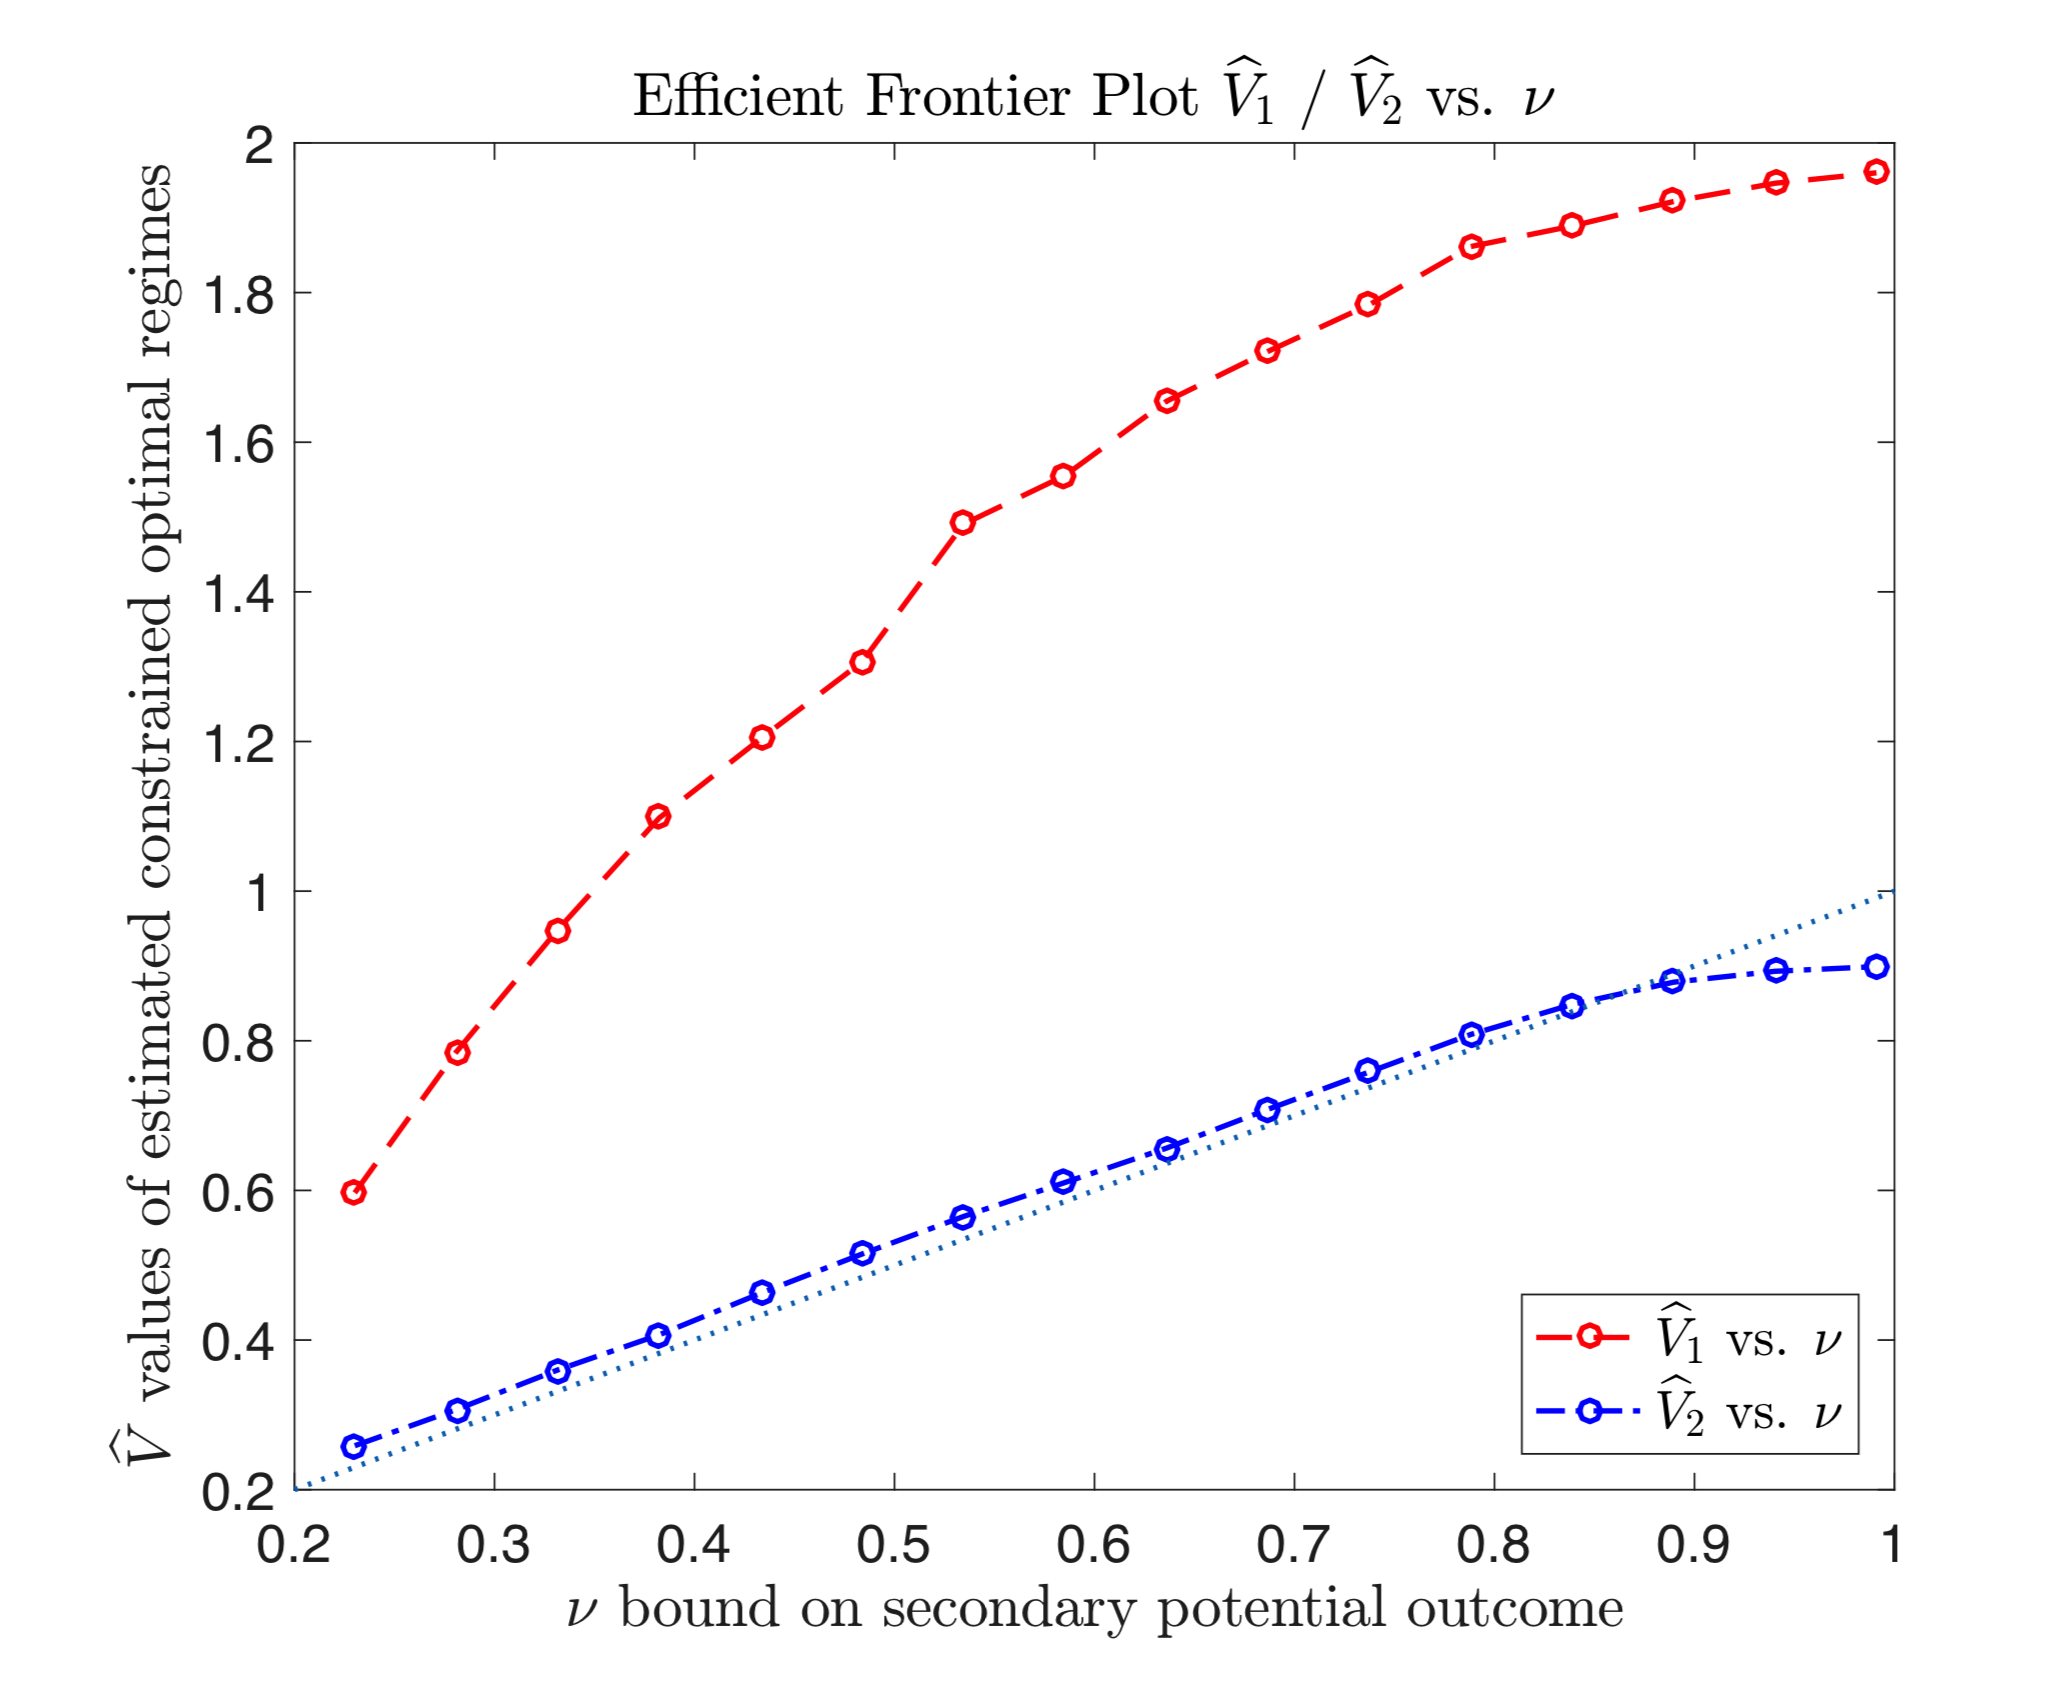
\includegraphics[width=.9\linewidth]{./Chapter-1/figs/efficient_plot1.png}
	\caption{Efficient frontier for estimated constrained optimal regimes (single-stage) for Setting 1.}
	\label{fig:1}
\justify
X-axis is for the values for the constraints $\nu$; Y-axis is for the values of estimated regimes. Red dashed line is for the values in terms of the primary outcome of interest. Blue dashed line is for the values in terms of the secondary outcome of interest.
\end{figure}


\section{Conclusion}
Most of the research in dynamics treatment regimes has been focusing on optimizing a single scalar outcome. However, it may be an oversimplification of the goals of practical clinical decision making. In this chapter, a new method is proposed to handle multiple competing outcomes. We cast estimation of an optimal treatment regime with competing outcomes as a constrained optimization problem, which maximizes the primary outcome of interest, subject to the constraints on the secondary outcomes of interest. We prove that our estimator of a constrained optimal treatment regime is consistent under mild regularity conditions. The asymptotic limiting distribution is derived for the estimated indexing parameter for the estimated optimal regimes. Our efficient frontier plots provide an intuitive way for clinicians to examine the trade-off between multiple competing outcomes. 



		

\chapter{Multi-stage Constrained Optimal Treatment Regimes}
\label{chap-two}
%set-up

\section{Introduction}
Dynamic treatment regimes (DTRs), also known as adaptive treatment strategies or policies, are sequences of decision rules of which input is time-varying patient information and output is a recommended treatment at each intervention point~\cite{Chakraborty2014, Moodie2004, Murphy2003}. These decision rules can be used to inform treatment decision for chronic conditions, e.g., depression, alcohol and drug abuse, HIV infection, cancer, diabetes etc., where clinicians have to make decisions at each stage based on evolving patient histories. A handful of methods have been developed to estimate the optimal treatment regimes. For example, indirect methods include Q-learning~\cite{Nahum2012}, penalized Q-learning~\cite{Song2011}, interactive Q-learning~\cite{Linn2014}, A-learning~\cite{Schulte2014}, regret-regression~\cite{henderson2010}, g-estimation~\cite{gestimation} and so on. Policy search methods include marginal structural mean models~\cite{Robins2000,Orellana2010a}, outcome weighted learning~\cite{Zhao2012,Zhang2012,Zhao2015}, doubly robust estimators~\cite{Zhang2012b}, and so forth. However, these methods only take a single clinical outcome into consideration, and neglect the clinical need to balance several competing outcomes. For example, a clinician may have to balance treatment effectiveness, side-effect burden, and cost while developing a treatment strategy for a patient with a chronic disease; or maximize the expected time to an adverse event while controlling the variance of the time to the adverse event.\\

Although handling the trade-off among multiple competing outcomes is important in practice, there has been little work done on this issue.  Lizotte et al. proposed to compute the optimal treatment regimes of all the possible linear combinations of two competing outcomes~\cite{Lizotte2010}. However, only considering linear trade-off between two competing outcomes may not be sufficient to describe all possible patient preferences~\cite{LaberTwo2014}. Wang et al. considered a compound score or ``expert score" by numerically combining information on treatment efficacy, toxicity, and the risk of disease progression~\cite{Wang2012}. Unfortunately, it can be difficult to elicit a good composite outcome, and the quality of the estimated treatment regime maybe severely affect by the misspecification of a composite outcome~\cite{Laber2014}. Some methods do not require the formation of composite outcomes. For example, set-valued dynamic treatment regimes proposed by Laber et al. inputs current patient information and outputs a set of recommended treatments. Multiple treatments may included in the set recommended, unless there exists a treatment that is best across all outcomes. Domain expertise is needed for tie breaking when a set of several treatments are recommended. Also, it needs to specify ``clinically significant differences" for competing outcomes~\cite{LaberTwo2014}. \\

In this chapter, we continue the work previously done by Linn at el.~\cite{constrained}, and propose a new statistical framework to tackle the problem of balancing multiple competing outcomes using constrained estimation. By restricting the values of secondary ones, we search for the feasible regimes with the maximized value of the primary outcome, ie., constrained optimal regimes. This method is useful, for example, when the clinicians need to find an adaptive intervention strategy that maximize the effectiveness and controls the side-effect burden simultaneously. This chapter focuses on constrained optimal regimes under the multiple stage setting. Data are assumed to be from Sequential, Multiple Assignment, Randomized Trials~\cite{Lei2012}. Observational data can also fit in our framework if the additional assumptions about the treatment assignment mechanism are tenable. However, precaution is needed when using data from observational studies, as one key assumption, the no unmeasured confounder assumption, can not be verified~\cite{Chakraborty2013}. 

\section{Methodology}
\subsection{Define multi-stage constrained optimal treatment regimes }
\subsubsection{Dataset}
 The dataset is denoted by $$\{(\bs{X}_{1}^{i}, A_{1}^{i},\bs{X}_{2}^{i}, A_{2}^{i}, \cdots, \bs{X}_{T}^{i}, A_{T}^{i}, \bs{Y}^{i})\}_{i=1}^{n},$$ which is composed of $n$ identically, independently distributed patient trajectories\\ $\{(\bs{X}_{1}, A_{1},\bs{X}_{2}, A_{2}, \cdots, \bs{X}_{T}, A_{T}, \bs{Y})\}$. Capital letters denote random variables; lower case letters denote realized values of these random variables. Let $\bs{X}_1$ be a patient baseline covariate, $A_1$ be the first-stage treatment variable, $\bs{X}_2$ be the patient covariate collected between first decision point and second decision point, $A_2$ be the second-stage treatment variable. So on, and so forth. Finally, $\bs{X}_T$ is the patient intermediate outcomes collected at the final decision point $T$, $A_T$ is the treatment assignment at that time point, and $\bs{Y}$ is the final outcome vector. For $t = 1, \cdots, T$, $\bs{X}_t\in \bs{\ml{X}}_t \subseteq{\mb{R}^{p_t}}$, $A_{t} \in \ml{A}_t = \{ 1, 2, \cdots, m_t\}$, and $\bs{Y} \in \mb{R}^J$. The first component $Y_1$ denote the primary outcome of interest, which is coded so that larger values are more desirable. Meanwhile, $Y_2, \cdots, Y_J$ are the secondary outcomes of interest, which are coded so that lower is better. Let $\bs{H}_t$ denote the patient history information up to the decision point $t$, i.e., $\bs{H}^\itl_1 = (1, \bs{X}^\itl_1)$, $\bs{H}^\itl_2 = ( \bs{H}^\itl_1, A_1, \bs{X}^\itl_2)$, $\cdots$,  $\bs{H}^\itl_t = (\bs{H}^\itl_{t-1}, A_{t-1}, \bs{X}^\itl_t)$, $\cdots$, $\bs{H}^\itl_T = (\bs{H}^\itl_{T-1}, A_{T-1}, \bs{X}^\itl_T)$. Besides, let $\br{A}_t = (A_1, A_2, \cdots, A_t)$ denotes a sequence of treatment history up to time point $t$, and $\br{A}_t \in \br{\ml{A}_t}$, where $\br{\ml{A}_t} = \ml{A}_1 \times \ml{A}_2 \times \cdots \times \ml{A}_t$, $t =2 , \cdots, T$. %Note $\br{A}_1 = A_1$ and $\br{\ml{A}}_1 = \ml{A}_1$. %Besides, let $\bs{W}= (\bs{X}_{2},  \, A_{2}, \, \cdots,\, \bs{X}_{T},  \, A_{T}, \bs{Y})$. 
 
 \subsubsection{Potential outcomes}
 The potential outcome or counter-factual framework by Neyman, Rubin and Robins are adopted to identify the causal effect of a regime. The set of potential outcomes is $\bs{W}^* = \{ \bs{X}^*_2(a_1), \bs{X}^*_3(\br{a}_2), \cdots, \bs{X}^*_T(\br{a}_{T-1}), \bs{Y}^*_T(\br{a}_T), \text{for all } \br{a}_t \in \br{\ml{A}}_t, t=1, 2, \cdots, T \}$, where $\bs{X}^*_t(\br{a}_{t-1})$ is the potential outcome that would have been observed if the patient followed the treatment history sequence $\br{a}_{t-1}$. The following three necessary assumptions are necessary to connect  observed data with potential outcomes~\cite{Neyman, Rubin2005, Rubin1980, Robins1997, Hernan2006}.
 \begin{itemize}
 	\item \textit{B1. Consistency:}
 	 $\bs{Y} = \bs{Y}^*(\br{A}_T)$, and $\bs{X}_t = \bs{X}^*_t(\br{A}_{t-1})$, $t = 2, \cdots, T$.
 	\item \textit{B2. Sequential randomization assumption:}
 	$A_{t}  \indep \bs{W}^*  \mid \bs{H}_{t}$ for $t =1 ,2, \cdots, T$.
 	\item \textit{B3. Positivity assumption:} $\exists \, \epsilon_t > 0$, such that $\text{Pr}(A_t = a_t \mid \bs{H}_t=\bs{h}_t) > \epsilon_t$, for all $a_t \in \ml{A}_t$, $t=1, 2, \cdots, T$.
 \end{itemize}
B1) states that the intermediate and final outcomes observed equal to the patient's intermediate and final potential outcomes under the sequence of treatment actually assigned. It also implies no interference among individuals. B2) mean that conditional on the observed patient history $\bs{H}_t$, the treatment at time point $t$ is assigned independently of the his or her potential outcomes. B3) guarantees a positive possibility for any $a_t \in \ml{A}_t$ having been assigned to patients with $\bs{H}_t = \bs{h}_t$. These assumptions imply that $\txt{Pr}(\bs{Y}^*(\br{a}_T) \le \bs{y} \,| \, \bs{H}^*_T(\br{a}_{T-1}) =\bs{h}_T) = \txt{Pr}(\bs{Y} \le \bs{y} \, |\,  \bs{H}_T = \bs{h}_T, A_T=a_T)$ and $\txt{Pr}(\bs{X}_{t+1}^*(\br{a}_{t}) \le \bs{x}_{t+1} \,|\, \bs{H}^*_t(\br{a}_{t-1}) = \bs{h}^*_t) = \txt{Pr}(\bs{X}_{t+1} \le \bs{x}_{t+1} \mid  \bs{H}_t = \bs{h}_t, A_t=a_t)$ for $t = 1, 2, \cdots, T-1$. Hence, we can estimate the values of a regime using the observed dataset.
\subsubsection{Define constrained optimal dynamic treatment regimes }
A dynamic treatment regime, $\bs{\pi} = (\pi_1, \pi_2, \cdots, \pi_T)$, is a sequence of decision rules. Each decision rule, $\pi_t : \text{supp}( \bs{H}_t ) \to \ml{A}_t$, is a function that maps the support of patient history information $\bs{H}_t$ to the set of all possible treatments at time point $t$. The final potential outcome under the regime $\bs{\pi}$ is $\bs{Y}^*(\bs{\pi}) = \sum_{\br{a}_T \in \br{\ml{A}}_T}\bs{Y}^*(\br{a}_T)\mb{I}(\bs{\pi} = \br{a}_T)$, and the intermediate potential outcome under that regime is $\bs{X}_{t+1}^*(\bs{\pi}_{t}) = \sum_{\br{a}_t \in \br{\ml{A}}_t}\bs{X}_{t+1}^*(\br{a}_{t})\mb{I}(\bs{\pi}_t = \br{a}_t)$, where $\bs{\pi}_t = (\pi_1, \pi_2, \cdots, \pi_t)$. The value of a dynamic treatment regime, $\bs{V}(\bs{\pi}) = \mb{E}\bs{Y}^*(\bs{\pi})$, is defined as the expected final outcome if each patient in the population of interest is treated according to $\bs{\pi}$. Each component of $\bs{V}(\bs{\pi})$ is denoted by $V_j(\bs{\pi}) = \mb{E}Y_j^*(\bs{\pi})$, for $j = 1, \cdots, J$. Our goal is to find a constrained optimal regime, $\bs{\pi}_{\bs{\nu}}^{*}$, that maximizes the expectation of the primary final potential outcome $V_1\left( \bs{\pi}\right) $, subject to an upper bound constraints on the expectation of the secondary final potential outcomes $V_j\left( \bs{\pi}\right)$, for $j=2 ,\cdots, J$.  The $J-1$ dimensional vector of upper bounds is denoted as $\bs{\nu} = (\nu_1, \nu_2, \cdots, \nu_{J-1})$, which can be determined by the preference of clinicians or patients.  Therefore, a multi-stage constrained optimal regime problem is defined as
\begin{equation}
\begin{gathered}
 \underset{\bs{\pi} \in \bs{\Pi}}{\txt{max}} \,\,
 V_1( \bs{\pi} )  \\
  \txt{subject to}  \,\, V_j( \bs{\pi} ) \le \nu_{j-1},
\end{gathered}
\end{equation}
where $j = 2, 3, \cdots, J$  and $\bs{\Pi}$ is the class of dynamic treatment regimes under consideration. The feasible space of the class of regimes, $\ml{F}(\bs{\Pi})$, is the set of all regimes satisfying the constraints. For each $\bs{\pi} \in \ml{F}(\bs{\Pi})$, $V_j(\bs{\pi}) \le \nu_{j-1}$, for $j = 2, \cdots, J$. Then, a multi-stage constrained optimal regime can also be written as $\bs{\pi}_{\bs{\nu}}^*= \text{argmax}_{{\bs{\pi} \in \ml{F}(\bs{\Pi})}}V_1 (\bs{\pi})$.\\

We choose the class of regime to be the class of linear decision rules, where each mapping function $\pi_t$ at time point $t$ is indexed by $\bs{\theta}_t$. More specifically, $\pi_t(\bs{h}_t) = \tsgn(\bs{h}^{\itl}_t\bs{\theta}_t)$. Hence, all $V_j(\bs{\pi})$'s can be considered as functions of $\bs{\theta}$ and can be exchangeably denoted $V_j(\bs{\theta})$'s. As only the directions of $\bs{h}^\itl_t\bs{\theta}_t$ matters, we restrict $\bs{\theta}_t$ to be unit vectors, i.e., $\bs{\theta}^\itl_t\bs{\theta}_t = 1$, for $t = 1, \cdots, T$. Then, problem (2.1) above can be written as
\begin{equation}
\begin{gathered}
\max_{\bs{\theta} \in \bs{\Theta}} V_1(\bs{\theta})\\
\,\, \txt{subject to}\,
V_j(\bs{\theta}) - \nu_j \le 0,\\
\hspace{2.0cm} \bs{\theta}_t^\itl \bs{\theta}_t^\itl - 1 =0.
\end{gathered}
 \end{equation}
where $\bs{\theta} = (\bs{\theta}_1, \cdots, \bs{\theta}_T)$, $j =2, \cdots, J$ and $t = 1, \cdots, T$. Let the feasible set of $\bs{\Theta}$ be $\ml{F}(\bs{\Theta})$, such that $V_j(\bs{\theta}) \le \nu_j$,  for any $\bs{\theta} \in \ml{F}(\bs{\Theta})$ and $j = 2, \cdots, J$. Then, the corresponding index parameter of a constrained optimal dynamic treatment regime is $\bs{\theta}^*_{\bs{\nu}} =\text{argmax}_{\bs{\theta} \in \ml{F}(\bs{\Theta})}V_1(\bs{\theta})$, and $\bs{\theta}^*_{\bs{\nu}} = (\bs{\theta}^*_{\bs{\nu},1}, \bs{\theta}^*_{\bs{\nu},2}, \cdots, \bs{\theta}^*_{\bs{\nu},T})$.

\begin{comment}
\textbf{ Convergence of the Penalty-Barrier Trajectory  $\bs{\theta}^*_{\kappa}(\mu)$  to $\bs{\tau}^0_{\kappa}$}\\

\textbf{ Convergence in probabilty of the estimator  to $\hat{\bs{\tau}}_{\kappa}(\mu)$ to  the Penalty-Barrier Trajectory  $\bs{\tau}^*_{\kappa}(\mu)$} \\

%\mnote{ convergence $\hat{\tau}_{\kappa}(\mu) \overset{p}{\to} \tau^*_{\kappa}(\mu) \to  \tau^0_{\kappa}(\mu)$}

Step 1:  $\underset{\bs{\tau}, \| \bs{\tau}_1 \|^2 = 1, \| \bs{\tau}_2 \|^2 = 1}{\sup} \mid \hat{S} (\bs{\tau}, \mu) -S^*( \bs{\tau}, \mu)  \mid = o_p(1)$ \\

Let $S^*(\bs{\tau}, \mu) = \mb{E} Y^*(\bs{\tau}) + \mu \txt{log} \lt\{ \kappa - \mb{E} Z^*(\bs{\tau}) \rt\} - \frac{1}{2\mu} \lt\{ (\bs{\tau}_1^\itl \bs{\tau}_1 -1 )^2 + (\bs{\tau}_2^\itl \bs{\tau}_2 -1 )^2 \rt\},$ and $\widehat{S}(\bs{\tau}, \mu) = \wh{\mb{E}} Y(\bs{\tau}) + \mu \, \txt{log} \lt\{ \kappa - \wh{\mb{E}}Z(\bs{\tau}) \rt\} - \frac{1}{2\mu} \lt\{ (\bs{\tau}_1^\itl \bs{\tau}_1 -1 )^2 + (\bs{\tau}_2^\itl \bs{\tau}_2 -1 )^2 \rt\},$ then
$$\widehat{S}(\bs{\tau}, \mu) - S^*(\bs{\tau}, \mu) = \hat{\mb{E}} Y(\bs{\tau}) - \mb{E} Y^*(\bs{\tau})  + \mu \, \txt{log}\frac{ \kappa - \hat{\mb{E}}Z(\bs{\tau})}{ \kappa - \mb{E} Z^*(\bs{\tau})}$$

First look at $\hat{\mb{E}} Y_n(\bs{\tau}) - \mb{E} Y^*(\bs{\tau})$

$Y_n(\bs{\tau}) \sim F_{Y_n}(y;\bs{\tau})$

If $Y_n(\bs{\tau}) \overset{d}{\to} Y^*(\bs{\tau})$, aka, $\wh{F}_{Y_n}(y;\bs{\tau}) \to F_Y(y;\bs{\tau}), \text{as } n \to \infty$, for all $y$ at which $F_Y(\cdot, \bs{\tau})$ is continuous. Also,  for each $\bs{\tau}$, if there exists some random variable $T$, such that  $|Y_n(\bs{\tau})| \le |T|$ for all $n$ and $\mb{E} |T| \le \infty$, then $\wh{\mb{E}} Y_n(\bs{\tau}) \to \mb{E} Y^*(\bs{\tau})$.
Thus, we have $\wh{\mb{E}} Y_n(\bs{\tau}) - \mb{E} Y^*(\bs{\tau}) = o_p(1)$ \\

Step 2:  conditions for $\wh{F}_{Y_n}(y;\bs{\tau}) \to F_Y(y;\bs{\tau}), \text{as } n \to \infty$\\

Step 3:  Consistency of $\wh{\bs{\tau}}_{n,\kappa} \to \bs{\tau}^*_{\kappa}$. It can be proven by following similar proof in Lemma 2 at one-stage. \\

Step 4: Asymptotic Normality of $\wh{\bs{\tau}}_{n,\kappa}$ \\
Taylor expansion, for each $\mu$ \\

$\nabla\wh{S}(\bs{\tau}^*_{\bs{\nu}}(\mu)) = \nabla\wh{S}(\wh{\bs{\tau}}_{\bs{\nu}}(\mu)) - \nabla^2\wh{S}(\tilde{\bs{\tau}}_{\bs{\nu}}(\mu) ) (\wh{\bs{\tau}}_{\bs{\nu}}(\mu) - \bs{\tau}^*_{\bs{\nu}}(\mu) )$


$\sqrt{n}\nabla\wh{S}(\bs{\tau}^*_{\bs{\nu}}(\mu)) =  -\sqrt{n} \nabla^2\wh{S}(\tilde{\bs{\tau}}_{\bs{\nu}}(\mu) ) (\wh{\bs{\tau}}_{\bs{\nu}}(\mu) - \bs{\tau}^*_{\bs{\nu}}(\mu) )$

\begin{flalign*}
\nabla\wh{S}(\bs{\tau}^*_{\bs{\nu}}(\mu)) = \nabla \mb{E} Y(\bs{\tau}) - \mu \frac{\nabla \mb{E} Z(\bs{\tau})}{  \kappa - \mb{E} Z(\bs{\tau}) }
\end{flalign*}

\begin{flalign*}
\nabla^2\wh{S}(\bs{\tau}^*_{\bs{\nu}}(\mu)) = \nabla^2 \mb{E} Y(\bs{\tau}) - \mu \frac{\nabla^2 \mb{E} Z(\bs{\tau}) \lt[ \kappa - \mb{E} Z(\bs{\tau}) \rt] + \{ \nabla \mb{E} Z(\bs{\tau}) \}^2}{  \lt\{\kappa - \mb{E} Z(\bs{\tau}) \rt\}^2}
\end{flalign*}
\begin{flalign*}
& \nabla \wh{\mb{E}} Y(\bs{\tau})\\
= & \nabla\int y \,d \wh{F}_{Y(\bs{\tau})}(y) \\
= &  \nabla\int y \lt[ \,d \iint  F_{\epsilon}\lt\{ y - m_Y - \tsgn(r_2)c_Y\rt\}\,d G_{Y}\lt\{ m_Y, c_Y, r_2 \mid \bs{h}_1 , d_1(\bs{h}_1)\rt\} \,d F_{\bs{H}_1}(\bs{h}_1) \rt] \\
= &  \nabla\int y \lt[ \,d \iint  F_{\epsilon}\lt\{ y - m_Y - \tsgn(r_2)c_Y\rt\}\,d G_{Y}\lt\{ m_Y, c_Y, r_2 \mid \bs{h}_1 , d_1(\bs{h}_1)\rt\} \,d F_{\bs{H}_1}(\bs{h}_1) \rt]
\end{flalign*}
Assuming $d G_Y$ is correctly specified and is differentiable and continuous
\\

Step 5: Projected CI for $\wh{\mb{E}} Y_n(\wh{\bs{\tau}}_{n,\kappa})$

Is $d F - d \hat{F} = d(F - \hat{F})$ ??\\
Note:
convergence $\hat{\tau}_{\kappa}(\mu) \overset{p}{\to} \tau^*_{\kappa}(\mu) \to  \tau^0_{\kappa}(\mu)$
\begin{flalign*}
&  \hat{\mb{E}} Y(\bs{\tau}) - \mb{E} Y^*(\bs{\tau})  \\
= & \int y \,d \wh{F}_{Y_d} (y) - \int y \,d F_{Y^*_d} (y) \\
= &  \int y  \lt\{  \,d\wh{F}_{Y_d} (y) - \,d F_{Y^*_d} (y) \rt\}  \\
% = & \int y  \lt\{ \wh{f}_{Y_d} (y) - f_{Y^*_d} (y) \rt\} \,dy
\end{flalign*}
If for any arbitrary $\bs{d}$, $d F_{Y^*_{\bs{d}}} (y) $ is a density and $d\wh{F}_{Y_{\bs{d}}}(y)$ is a uniformly consistent estimator; that is $\underset{y}{\sup} \mid d\wh{F}_{Y_d} (y) - d F_{Y^*_d} (y) \mid =o_p(1)$, then

\begin{flalign*}
&  \hat{\mb{E}} Y(\bs{\tau}) - \mb{E} Y^*(\bs{\tau})  \\
= & \int y \,d \wh{F}_{Y_d} (y) - \int y \,d F_{Y^*_d} (y) \\
= &  \int y  \lt\{  \,d\wh{F}_{Y_d} (y) - \,d F_{Y^*_d} (y) \rt\}  \\
\le & \int \mid y \mid \, dy  \cdot o_p(1) \\
% = & \int y  \lt\{ \wh{f}_{Y_d} (y) - f_{Y^*_d} (y) \rt\} \,dy\\
= &  \iint  F_{\varepsilon_Y}\lt[ y - m(\bs{h}_2) - \tsgn\lt\{r_2(\bs{h}_2; \bs{\tau}_2)\rt\}c_Y(\bs{h}_2) \rt] \,d G_{Y}\lt\{ m_Y, c_Y, r_2 \rvert \bs{h}_1 , d_1(\bs{h}_1)\rt\} \,d F_{\bs{H}_1}(\bs{h}_1)
\end{flalign*}

\newpage
\textbf{Reference}\\

\textbf{Convergence in Distribution}\\
Suppose that $(X_1, X_2, \dots)$ and $X$ are real-valued random variables with distribution functions $(F_1, F_2,  \dots)$ and $F$, respectively. We say that the distribution of $X_n$ converges to the distribution of $X$ as $n \to \infty$ if
$$F_n(x) \to F(x), \text{as } n \to \infty$$
for all $x$ at which $F$ is continuous. \\
% Link https://www.probabilitycourse.com/chapter7/7_2_4_convergence_in_distribution.php

\textbf{Lebesgue's Dominated Convergence Theorem}\\
If for some random variable $Z$, $| X_n | \le | Z |$ for all $n$ and $\mb{E} | Z | \le \infty$, then $X_n \overset{d}{\to} X$ implies that $\mb{E} X_n \to \mb{E} X$.

\end{comment}

\begin{comment}
\textbf{ Convergence of the Penalty-Barrier Trajectory  $\bs{\tau}^*_{\kappa}(\mu)$  to $\bs{\tau}^0_{\kappa}$}\\

\textbf{ Convergence in probabilty of the estimator  to $\hat{\bs{\tau}}_{\kappa}(\mu)$ to  the Penalty-Barrier Trajectory  $\bs{\tau}^*_{\kappa}(\mu)$} \\

%\mnote{ convergence $\hat{\tau}_{\kappa}(\mu) \overset{p}{\to} \tau^*_{\kappa}(\mu) \to  \tau^0_{\kappa}(\mu)$}

Step 1:  $\underset{\bs{\tau}, \| \bs{\tau}_1 \|^2 = 1, \| \bs{\tau}_2 \|^2 = 1}{\sup} \mid \hat{S} (\bs{\tau}, \mu) -S^*( \bs{\tau}, \mu)  \mid = o_p(1)$ \\

Let $S^*(\bs{\tau}, \mu) = \mb{E} Y^*(\bs{\tau}) + \mu \txt{log} \lt\{ \kappa - \mb{E} Z^*(\bs{\tau}) \rt\} - \frac{1}{2\mu} \lt\{ (\bs{\tau}_1^\itl \bs{\tau}_1 -1 )^2 + (\bs{\tau}_2^\itl \bs{\tau}_2 -1 )^2 \rt\},$ and $\widehat{S}(\bs{\tau}, \mu) = \wh{\mb{E}} Y(\bs{\tau}) + \mu \, \txt{log} \lt\{ \kappa - \wh{\mb{E}}Z(\bs{\tau}) \rt\} - \frac{1}{2\mu} \lt\{ (\bs{\tau}_1^\itl \bs{\tau}_1 -1 )^2 + (\bs{\tau}_2^\itl \bs{\tau}_2 -1 )^2 \rt\},$ then
$$\widehat{S}(\bs{\tau}, \mu) - S^*(\bs{\tau}, \mu) = \hat{\mb{E}} Y(\bs{\tau}) - \mb{E} Y^*(\bs{\tau})  + \mu \, \txt{log}\frac{ \kappa - \hat{\mb{E}}Z(\bs{\tau})}{ \kappa - \mb{E} Z^*(\bs{\tau})}$$

First look at $\hat{\mb{E}} Y_n(\bs{\tau}) - \mb{E} Y^*(\bs{\tau})$

$Y_n(\bs{\tau}) \sim F_{Y_n}(y;\bs{\tau})$

If $Y_n(\bs{\tau}) \overset{d}{\to} Y^*(\bs{\tau})$, aka, $\wh{F}_{Y_n}(y;\bs{\tau}) \to F_Y(y;\bs{\tau}), \text{as } n \to \infty$, for all $y$ at which $F_Y(\cdot, \bs{\tau})$ is continuous. Also,  for each $\bs{\tau}$, if there exists some random variable $T$, such that  $|Y_n(\bs{\tau})| \le |T|$ for all $n$ and $\mb{E} |T| \le \infty$, then $\wh{\mb{E}} Y_n(\bs{\tau}) \to \mb{E} Y^*(\bs{\tau})$.
Thus, we have $\wh{\mb{E}} Y_n(\bs{\tau}) - \mb{E} Y^*(\bs{\tau}) = o_p(1)$ \\

Step 2:  conditions for $\wh{F}_{Y_n}(y;\bs{\tau}) \to F_Y(y;\bs{\tau}), \text{as } n \to \infty$\\

Step 3:  Consistency of $\wh{\bs{\tau}}_{n,\kappa} \to \bs{\tau}^*_{\kappa}$. It can be proven by following similar proof in Lemma 2 at one-stage. \\

Step 4: Asymptotic Normality of $\wh{\bs{\tau}}_{n,\kappa}$ \\
Taylor expansion, for each $\mu$ \\

$\nabla\wh{S}(\bs{\tau}^*_{\bs{\nu}}(\mu)) = \nabla\wh{S}(\wh{\bs{\tau}}_{\bs{\nu}}(\mu)) - \nabla^2\wh{S}(\tilde{\bs{\tau}}_{\bs{\nu}}(\mu) ) (\wh{\bs{\tau}}_{\bs{\nu}}(\mu) - \bs{\tau}^*_{\bs{\nu}}(\mu) )$


$\sqrt{n}\nabla\wh{S}(\bs{\tau}^*_{\bs{\nu}}(\mu)) =  -\sqrt{n} \nabla^2\wh{S}(\tilde{\bs{\tau}}_{\bs{\nu}}(\mu) ) (\wh{\bs{\tau}}_{\kappa,\mu} - \bs{\tau}^*_{\kappa,\mu} )$

\begin{flalign*}
\nabla\wh{S}(\bs{\tau}^*_{\kappa,\mu}) = \nabla \mb{E} Y(\bs{\tau}) - \mu \frac{\nabla \mb{E} Z(\bs{\tau})}{  \kappa - \mb{E} Z(\bs{\tau}) }
\end{flalign*}

\begin{flalign*}
\nabla^2\wh{S}(\bs{\tau}^*_{\kappa,\mu}) = \nabla^2 \mb{E} Y(\bs{\tau}) - \mu \frac{\nabla^2 \mb{E} Z(\bs{\tau}) \lt[ \kappa - \mb{E} Z(\bs{\tau}) \rt] + \{ \nabla \mb{E} Z(\bs{\tau}) \}^2}{  \lt\{\kappa - \mb{E} Z(\bs{\tau}) \rt\}^2}
\end{flalign*}
\begin{flalign*}
& \nabla \wh{\mb{E}} Y(\bs{\tau})\\
= & \nabla\int y \,d \wh{F}_{Y(\bs{\tau})}(y) \\
= &  \nabla\int y \lt[ \,d \iint  F_{\epsilon}\lt\{ y - m_Y - \tsgn(r_2)c_Y\rt\}\,d G_{Y}\lt\{ m_Y, c_Y, r_2 \mid \bs{h}_1 , d_1(\bs{h}_1)\rt\} \,d F_{\bs{H}_1}(\bs{h}_1) \rt] \\
= &  \nabla\int y \lt[ \,d \iint  F_{\epsilon}\lt\{ y - m_Y - \tsgn(r_2)c_Y\rt\}\,d G_{Y}\lt\{ m_Y, c_Y, r_2 \mid \bs{h}_1 , d_1(\bs{h}_1)\rt\} \,d F_{\bs{H}_1}(\bs{h}_1) \rt]
\end{flalign*}
Assuming $d G_Y$ is correctly specified and is differentiable and continuous
\\

Step 5: Projected CI for $\wh{\mb{E}} Y_n(\wh{\bs{\tau}}_{n,\kappa})$

Is $d F - d \hat{F} = d(F - \hat{F})$ ??\\
Note:
convergence $\hat{\tau}_{\kappa}(\mu) \overset{p}{\to} \tau^*_{\kappa}(\mu) \to  \tau^0_{\kappa}(\mu)$
\begin{flalign*}
&  \hat{\mb{E}} Y(\bs{\tau}) - \mb{E} Y^*(\bs{\tau})  \\
= & \int y \,d \wh{F}_{Y_d} (y) - \int y \,d F_{Y^*_d} (y) \\
= &  \int y  \lt\{  \,d\wh{F}_{Y_d} (y) - \,d F_{Y^*_d} (y) \rt\}  \\
% = & \int y  \lt\{ \wh{f}_{Y_d} (y) - f_{Y^*_d} (y) \rt\} \,dy
\end{flalign*}
If for any arbitrary $\bs{d}$, $d F_{Y^*_{\bs{d}}} (y) $ is a density and $d\wh{F}_{Y_{\bs{d}}}(y)$ is a uniformly consistent estimator; that is $\underset{y}{\sup} \mid d\wh{F}_{Y_d} (y) - d F_{Y^*_d} (y) \mid =o_p(1)$, then

\begin{flalign*}
&  \hat{\mb{E}} Y(\bs{\tau}) - \mb{E} Y^*(\bs{\tau})  \\
= & \int y \,d \wh{F}_{Y_d} (y) - \int y \,d F_{Y^*_d} (y) \\
= &  \int y  \lt\{  \,d\wh{F}_{Y_d} (y) - \,d F_{Y^*_d} (y) \rt\}  \\
\le & \int \mid y \mid \, dy  \cdot o_p(1) \\
% = & \int y  \lt\{ \wh{f}_{Y_d} (y) - f_{Y^*_d} (y) \rt\} \,dy\\
= &  \iint  F_{\varepsilon_Y}\lt[ y - m(\bs{h}_2) - \tsgn\lt\{r_2(\bs{h}_2; \bs{\tau}_2)\rt\}c_Y(\bs{h}_2) \rt] \,d G_{Y}\lt\{ m_Y, c_Y, r_2 \rvert \bs{h}_1 , d_1(\bs{h}_1)\rt\} \,d F_{\bs{H}_1}(\bs{h}_1)
\end{flalign*}

\newpage
\textbf{Reference}\\

\textbf{Convergence in Distribution}\\
Suppose that $(X_1, X_2, \dots)$ and $X$ are real-valued random variables with distribution functions $(F_1, F_2,  \dots)$ and $F$, respectively. We say that the distribution of $X_n$ converges to the distribution of $X$ as $n \to \infty$ if
$$F_n(x) \to F(x), \text{as } n \to \infty$$
for all $x$ at which $F$ is continuous. \\
% Link https://www.probabilitycourse.com/chapter7/7_2_4_convergence_in_distribution.php

\textbf{Lebesgue's Dominated Convergence Theorem}\\
If for some random variable $Z$, $| X_n | \le | Z |$ for all $n$ and $\mb{E} | Z | \le \infty$, then $X_n \overset{d}{\to} X$ implies that $\mb{E} X_n \to \mb{E} X$.

\end{comment}

% modeling conditional distributions


\subsection{Re-define constrained optimal regimes via penalization}
Problem (2.2) is a nonlinear constrained continuous optimization task. It is solved via interior point method, where we re-formalize  the problem via quadratic-barrier penalization. To re-formalize the problem, we let $v_1(\bs{\theta}) = -V_1(\bs{\theta})$ and $v_j(\bs{\theta}) = V_j(\bs{\theta}) - \nu_j$ for $j = 2, \cdots, J$. Moreover, $h_t(\bs{\theta}_t) = \bs{\theta}_t^{\itl}\bs{\theta}_t - 1$. Hence, we have problem (2.2) equivalent to the following
\begin{equation}
\begin{gathered}
\min_{\bs{\theta} \in \bs{\Theta}} v_1(\bs{\theta})\\
\txt{subject to } v_j(\bs{\theta}) \le 0, \\
\hspace{2.0cm}h_t(\bs{\theta}_t) = 0.
\end{gathered}
\end{equation}
where $\bs{\theta} = (\bs{\theta}_1, \cdots, \bs{\theta}_T)$, $j =1, \cdots, J$ and $t = 1, \cdots, T$ . Interior point method approximate the solution of problem (2.3) by solving a sequence of the following problem (2.4), where $\mu$ is positive and approaches to zero in the limit. For each $\mu > 0$, the approximate problem is 
\begin{equation}
\min_{\bs{\theta}, \bs{z}} \phi_{\mu}(\bs{\theta}, \bs{z}) = \min v_1(\bs{\theta}) - \mu \sum_{j=2}^J \ln z_j, \text{subject to}\,\, v_j(\bs{\theta}) +z_j = 0, h_t(\bs{\theta}_t) = 0
\end{equation}
where $j=2, \cdots, J$ and $t = 1, \cdots, T$. $z_j$'s are the slack variables, which are restricted to be positive due the $\ln$ operator. The logarithmic terms, $\ln z_j$'s, are the barrier functions, which enforce the solution path to be within the feasible region of the problem (2.3). More details on interior points method can be found at section 2.1.2. \\

The sequence of solutions to problem (2.4) forms a trajectory path $\lt\{\bs{\theta}^*_{\nu}(\mu)\rt\}_{\mu\to0+}$ that convergence to the solution to problem (2.3) as $\mu \to 0$, i.e., $\lim_{\mu \to 0}\bs{\theta}^*_{\bs{\nu}}(\mu)=\bs{\theta}^*_{\bs{\nu}}$. The conditions for its convergence can be found at section 2.1.3. Let $\wh{\bs{V}}(\theta)$ be a consistent estimator of the values of a regime $\pi$. Then, correspondingly, $\wh{v}_1(\bs{\theta}) = -\wh{V}_1(\bs{\theta})$ and $\wh{v}_j(\bs{\theta})=\wh{\bs{V}}_j(\bs{\theta}) -\nu_j$ for $j = 2, \cdots, J$. Then, problem (2.4) with the plugin estimator is
\begin{equation}
\min_{\bs{\theta}, \bs{z}} \wh{\phi}_{\mu}(\bs{\theta}, \bs{z}) = \min \wh{v}_1(\bs{\theta}) - \mu \sum_{j=2}^J \ln z_j, \text{ subject to}\,\, \wh{v}_j(\bs{\theta}) +z_j = 0, h_t(\bs{\theta}_t) = 0,
\end{equation}
for $j=2, \cdots, J$ and $t=1, \cdots, T$. The solution to problem (2.5) is equivalent to the solution to penalty-barrier function below. 
\begin{equation}
\min_{\bs{\theta}} \wh{\phi}^{BP}_{\mu}(\bs{\theta}) = \min \wh{v}_1(\bs{\theta}) - \mu \sum_{j=2}^J \ln (-\wh{v}_j(\bs{\theta})) + \frac{1}{2\mu}\sum_{t=1}^{T}(\bs{\theta}^{\itl}_t\bs{\theta}_t - 1)^2
\end{equation}
Denote the solution to (2.5/2.6) as $\wh{\bs{\theta}}_{\nu}(\mu)$.We have proven that $\wh{\bs{\theta}}_{\nu}(\mu) \overset{p}{\to} \bs{\theta}^*_{\nu}(\mu)$. For the consistency of this estimator, the details and proof are provided in section 2.1.4 and appendix A.2.
\begin{comment}
\subsection{Convergence of penalty-barrier trajectory  $\bs{\theta}^*_{\bs{\nu}}(\mu)$}

We again examine the conditions under which the penalty-barrier trajectory $\bs{\tau}^*_{\kappa}(\mu)$ converges to the original constrained maximizer $\bs{\tau}^0_{\kappa}$, of which details are provided Appendix 1 Proof Draft 1. We specify  the conditions need(2.ed for our problem as follows. For notation simplicity in this section, we let $f(\bs{\tau}) = \mb{E} Y^*(\bs{\tau})$, $c_1 (\bs{\tau}) = \kappa - \mb{E}Z^*(\bs{\tau})$, $c_2(\bs{\tau}) = \bs{\tau}_1^\itl \bs{\tau}_1 - 1$, and $c_3(\bs{\tau}) = \bs{\tau}_2^\itl \bs{\tau}_2 - 1$. Let $g(\bs{\tau})$ denote the gradient of $f(\bs{\tau})$, i.e., $g(\bs{\tau}) = \nabla f(\bs{\tau}) = \nabla \mb{E}Y^*(\bs{\tau})$. Also, let $\bs{c}(\bs{\tau})$ be the vector of constraint functions $\{c_i(\bs{\tau})\}$, $i = 1, 2, 3$. The Jacobian matrix $\bs{c}^{\prime}(\bs{\tau})$ of first derivative of $\bs{c}(\bs{\tau})$ has row $\{\nabla c_{i}(\bs{\tau})\}^{\itl}$, and we use $J(\bs{\tau})$ to denote this Jacobian for concise.\\
 \begin{lemma}[Conditions for the trajectory $\{ \bs{\tau}_{\kappa}^*(\mu) \}$ converging to $\bs{\tau}^0_{\kappa}$\cite{Nocedal1999,fiacco,Forsgren2002}]
	Assume
	\begin{enumerate}
		\item the functions $f$, $c_1$, $c_2$, and $c_3$ are twice differentiable with respect to $\bs{\tau}$;
		\item the gradients $\nabla c_1$, $\nabla c_2$, and $\nabla c_3$ are linearly independent, where the gradients are taken with respect to $\bs{\tau}$;
		\item strict complementarity holds for  $\lambda_1^0 c_1(\bs{\tau}_{\kappa}^0) = 0$, where $\lambda_1^0$ is the Lagrangian multiplier of the inequality constraint $c_1$;
		\item the sufficient conditions under which $\bs{\tau}_{\kappa}^0$ be an isolated local constrained minimum of Problem (2) are satisfied by $(\bs{\tau}^0_{\kappa}, \bs{\lambda}^{0})$, where $\bs{\lambda}^0 = (\lambda_1^0, \lambda_2^0, \lambda_3^0)^\itl $ of which $\lambda_2^0$ is the  Lagrangian multipliers for the  constraint $c_2$, and $\lambda_3$ for $c_3$. The sufficient conditions for optimality are
		\begin{enumerate}
			\item $\bs{\tau}_{\kappa}^0$ is feasible and the LICQ (Linear Independence Constraint Qualification) holds at $\bs{\tau}_{\kappa}^0$, i.e., the Jacobian matrix of active constraints at $\bs{\tau}_{\kappa}^0$, $J_{\mathcal{A}}(\bs{\tau}_{\kappa}^0)$, has full row rank;
			\item $\bs{\tau}_{\kappa}^0$ is a KKT point and strict complementarity holds, i.e, the (necessarily unique) multiplier $\bs{\lambda}^0$ has the property that $\lambda_i^0 > 0$, for all $i  \in \mathcal{A}_{\mathcal{I}}(\bs{\tau}_{\kappa}^0)$, the set of indices of active inequality constraints at $\bs{\tau}_{\kappa}^0$;
			\item for all nonzero vectors $\bs{p}$ satisfying $J_{\mathcal{A}}(\bs{\tau}_{\kappa}^0)\bs{p} = 0$, there exists $\omega > 0$ such that $\bs{p}^{\intercal}H(\bs{\tau}_{\kappa}^0, \bs{\lambda}^0) \bs{p} \ge \omega \|\bs{p}\|^2$., where $H(\bs{\tau}_{\kappa}^0, \bs{\lambda}^0) $ is the hessian of the Lagrangian at $\bs{\tau}_{\kappa}^0$ and $\bs{\lambda}^0$, where $\bs{\lambda}^0$ is the vector of the Lagrangian multipliers, $\bs{\lambda}^0 = (\lambda_1^0, \lambda_2^0, \lambda_3^0)^{\intercal}$.
		\end{enumerate}
		then there is a positive neighborhood about $\mu = 0$ for which a unique-isolated differentiable function $\bs{\tau}^*_{\kappa}(\mu)$ exists. It describes a unique isolated trajectory of local maxima of $S^*(\bs{\tau}, \mu)$, where $\bs{\tau}^*_{\kappa}(\mu) \to \bs{\tau}^0_{\kappa}$ as $\mu \to 0$.
	\end{enumerate}
\end{lemma}

To find $\bs{\tau}^*_{\kappa}(\mu)$, we need to examine its stationarity. That is $\nabla S^*(\bs{\tau}, \mu) = 0$ is satisfied at $\bs{\tau}^*_{\kappa}(\mu)$. Its equivalent system of non-linear equations is
\begin{align*}
F^{\mu}(\bs{\tau}, \bs{\lambda}) =
\begin{pmatrix} g(\bs{\tau}) - J(\bs{\tau}) \bs{\lambda} \\ c_1( \bs{\tau}) \lambda_1 - \mu \\ c_2(\bs{\tau}) + \mu \lambda_2\\ c_3(\bs{\tau}) + \mu \lambda_3 \end{pmatrix} = 0
\end{align*}
We also define $\chi_1 \triangleq \sfrac{\mu}{c_1(\bs{\tau})}$, $\chi_2 \triangleq - \sfrac{c_2(\bs{\tau})}{\mu}$ and $\chi_3 \triangleq - \sfrac{c_3(\bs{\tau})}{\mu}$ which can be considered as approximates of the Lagrangian multipliers under  $\mu$-perturbed KKT conditions. \\
\end{comment}
\begin{comment}
Is $d F - d \hat{F} = d(F - \hat{F})$ ??\\
Note:
convergence $\hat{\tau}_{\kappa}(\mu) \overset{p}{\to} \tau^*_{\kappa}(\mu) \to  \tau^0_{\kappa}(\mu)$
\begin{flalign*}
&  \hat{\mb{E}} Y(\bs{\tau}) - \mb{E} Y^*(\bs{\tau})  \\
= & \int y \,d \wh{F}_{Y_d} (y) - \int y \,d F_{Y^*_d} (y) \\
= &  \int y  \lt\{  \,d\wh{F}_{Y_d} (y) - \,d F_{Y^*_d} (y) \rt\}  \\
% = & \int y  \lt\{ \wh{f}_{Y_d} (y) - f_{Y^*_d} (y) \rt\} \,dy
\end{flalign*}
If for any arbitrary $\bs{d}$, $d F_{Y^*_{\bs{d}}} (y) $ is a density and $d\wh{F}_{Y_{\bs{d}}}(y)$ is a uniformly consistent estimator; that is $\underset{y}{\sup} \mid d\wh{F}_{Y_d} (y) - d F_{Y^*_d} (y) \mid =o_p(1)$, then

\begin{flalign*}
&  \hat{\mb{E}} Y(\bs{\tau}) - \mb{E} Y^*(\bs{\tau})  \\
= & \int y \,d \wh{F}_{Y_d} (y) - \int y \,d F_{Y^*_d} (y) \\
= &  \int y  \lt\{  \,d\wh{F}_{Y_d} (y) - \,d F_{Y^*_d} (y) \rt\}  \\
\le & \int \mid y \mid \, dy  \cdot o_p(1) \\
% = & \int y  \lt\{ \wh{f}_{Y_d} (y) - f_{Y^*_d} (y) \rt\} \,dy\\
= &  \iint  F_{\varepsilon_Y}\lt[ y - m(\bs{h}_2) - \tsgn\lt\{r_2(\bs{h}_2; \bs{\tau}_2)\rt\}c_Y(\bs{h}_2) \rt] \,d G_{Y}\lt\{ m_Y, c_Y, r_2 \rvert \bs{h}_1 , d_1(\bs{h}_1)\rt\} \,d F_{\bs{H}_1}(\bs{h}_1)
\end{flalign*}

\textbf{Reference}\\

\textbf{Convergence in Distribution}\\
Suppose that $(X_1, X_2, \dots)$ and $X$ are real-valued random variables with distribution functions $(F_1, F_2,  \dots)$ and $F$, respectively. We say that the distribution of $X_n$ converges to the distribution of $X$ as $n \to \infty$ if
$$F_n(x) \to F(x), \text{as } n \to \infty$$
for all $x$ at which $F$ is continuous. \\
% Link https://www.probabilitycourse.com/chapter7/7_2_4_convergence_in_distribution.php

\textbf{Lebesgue's Dominated Convergence Theorem}\\
If for some random variable $Z$, $| X_n | \le | Z |$ for all $n$ and $\mb{E} | Z | \le \infty$, then $X_n \overset{d}{\to} X$ implies that $\mb{E} X_n \to \mb{E} X$.


% modeling conditional distributions
\subsection{Consistency of $\wh{\bs{\theta}}_{\bs{\nu}}(\mu)$}
\textbf{ Convergence in probabilty of the estimator  to $\hat{\bs{\tau}}_{\kappa}(\mu)$ to  the penalty-barrier trajectory  $\bs{\tau}^*_{\kappa}(\mu)$} \\
Here, we examine the consistency of $\widehat{\bs{\tau}}_{\kappa}(\mu)$  to $\bs{\tau}^*_{\kappa}(\mu)$, and the following lemmas are needed. As $S^*(\bs{\tau}, \mu) = \mb{E} Y^*(\bs{\tau}) + \mu \txt{log} \lt\{ \kappa - \mb{E} Z^*(\bs{\tau}) \rt\} - \frac{1}{2\mu} \lt\{ (\bs{\tau}_1^\itl \bs{\tau}_1 -1 )^2 + (\bs{\tau}_2^\itl \bs{\tau}_2 -1 )^2 \rt\},$ and $\widehat{S}(\bs{\tau}, \mu) = \wh{\mb{E}} Y_n(\bs{\tau}) + \mu \, \txt{log} \lt\{ \kappa - \wh{\mb{E}}Z_n(\bs{\tau}) \rt\} - \frac{1}{2\mu} \lt\{ (\bs{\tau}_1^\itl \bs{\tau}_1 -1 )^2 + (\bs{\tau}_2^\itl \bs{\tau}_2 -1 )^2 \rt\},$ then
$$\widehat{S}(\bs{\tau}, \mu) - S^*(\bs{\tau}, \mu) = \wh{\mb{E}} Y_n(\bs{\tau}) - \mb{E} Y^*(\bs{\tau})  + \mu \, \txt{log}\frac{ \kappa - \wh{\mb{E}}Z_n(\bs{\tau})}{ \kappa - \mb{E} Z^*(\bs{\tau})}$$
For notation simplicity, we denote $Pr\lt\{ Y^*\lt(\bs{d}\rt) \le y \rt\} = F_{ Y^*(\bs{\tau})}(y)$ and $Pr\lt\{ Z^*\lt(\bs{d}\rt) \le z \rt\} = F_{ Z^*(\bs{\tau})}(z)$. Their estimators are denoted by $\wh{Pr}\lt\{ Y_n\lt(\bs{d}\rt) \le y \rt\} = \wh{F}_{ Y_n(\bs{\tau})}(y)$ and  $\wh{Pr}\lt\{ Z_n\lt(\bs{d}\rt) \le z \rt\} = \wh{F}_{ Z_n(\bs{\tau})}(z)$ . Also, $Y^*(\bs{\tau})$ denotes the random variable with the cumulative distribution function $F_{ Y^*(\bs{\tau})}(y)$, and  $Y_n(\bs{\tau})$ denotes the random variable with the cumulative distribution function $\wh{F}_{ Y_n(\bs{\tau})}(y)$. Same applies to $Z^*(\bs{\tau})$ and  $Z_n(\bs{\tau})$.
\begin{lemma}
	For any fixed $\bs{\tau}: \bs{\tau}_1^\itl\bs{\tau}_1 - 1 = 0$, and $\bs{\tau}_2^\itl\bs{\tau}_2 -1 = 0$. We assume that, for each $\bs{\tau}$,
	\begin{enumerate}
		\item $Y_n(\bs{\tau}) \overset{d}{\to} Y^*(\bs{\tau})$, i.e., $\nlim \wh{F}_{Y_n({\bs{\tau}})}(y) = F_{Y^*({\bs{\tau}})}(y)$, for all $y$ at which $F_{Y^*(\bs{\tau})}(y)$ is continuous;
		\item If there exists some random variable $T$, such that  $|Y_n(\bs{\tau})| \le |T|$ for all $n$ and $\mb{E} |T| \le \infty$,
	\end{enumerate}
	Also, we assume the same assumptions for $Z({\bs{\tau}})$.
	Then, we have\\
	\begin{flalign*}
	\underset{\bs{\tau}:\bs{\tau}_1^\itl \bs{\tau}_1=1, \bs{\tau}_2^\itl \bs{\tau}_2=1}{\sup}\left|\widehat{S}_{\kappa}(\bs{\tau}, \mu)-S^*_{\kappa}(\bs{\tau},  \mu)\right|=o_{p}(1).
	\end{flalign*}
\end{lemma}
\begin{proof}
	For any fixed $\bs{\tau}: \bs{\tau}_1^\itl\bs{\tau}_1 = 1$ and $\bs{\tau}_2^\itl\bs{\tau}_2 = 1$, we have
	\begin{flalign*}
	& \widehat{S}_{\kappa}(\bs{\tau}, \mu)-S_{\kappa}^{*}(\bs{\tau}, \mu)\\
	= &\, \wh{\mb{E}} Y_n(\bs{\tau}) - \mb{E} Y^*(\bs{\tau}) + \mu \txt{log} \lt\{ \frac{ \kappa - \wh{\mb{E}} Z(\bs{\tau}) }{ \kappa - \mb{E} Z^*(\bs{\tau}) }\rt\}\\
	= &\, \int y \,d \wh{F}_{Y(\bs{\tau})}(y)- \int y \,d F_{Y^*(\bs{\tau})}(y)+ \mu \txt{log} \lt\{ \frac{ \kappa - \int z \,d \wh{F}_{Z_n(\bs{\tau})}(z)}{ \kappa - \int z \,d F_{Z^*(\bs{\tau})}(z) }\rt\}
	\end{flalign*}
	
	For $\wh{\mb{E}} Y_n(\bs{\tau}) - \mb{E} Y^*(\bs{\tau})$, we have $Y_n(\bs{\tau}) \sim \wh{F}_{Y_n(\bs{\tau})}(y)$, and $Y^*(\bs{\tau}) \sim F_{Y^*(\bs{\tau})}(y)$. Under the assumptions 1 and 2, %if $Y_n(\bs{\tau}) \overset{d}{\to} Y^*(\bs{\tau})$, aka, $\wh{F}_{Y_n(\bs{\tau})}(y) \to F_{Y^*(\bs{\tau})}(y), \text{as } n \to \infty$, for all $y$ at which $F_{Y^*(\bs{\tau})}(y)$ is continuous. Also,  for each $\bs{\tau}$, if there exists some random variable $T$, such that  $|Y_n(\bs{\tau})| \le |T|$ for all $n$ and $\mb{E} |T| \le \infty$,
	by dominated convergence theorem, we have
	%$\wh{\mb{E}} Y_n(\bs{\tau}) - \mb{E} Y^*(\bs{\tau}) = o_p(1)$ ,
	we have $\underset{n \to \infty}{\lim}\wh{\mb{E}} Y_n(\bs{\tau}) = \mb{E} Y^*(\bs{\tau})$. Similarily, we have  $\underset{n \to \infty}{\lim}\wh{\mb{E}} Z_n(\bs{\tau}) = \mb{E} Z^*(\bs{\tau})$.  The two terms embedded in log operator are forced to be strictly greater than zero.  Together with continuous mapping theorem, we have
	\begin{flalign*}
	\widehat{S}_{\kappa}(\bs{\tau}, \mu)-S_{\kappa}(\bs{\tau}, \mu) =o_p(1).
	\end{flalign*}
	As this holds for any fixed value of $\bs{\tau}$ and constants $\mu$ sufficiently small, we have
	$$\underset{\bs{\tau}:\bs{\tau}_1^\itl \bs{\tau}_1=1, \bs{\tau}_2^\itl \bs{\tau}_2=1}{\sup}\left|\widehat{S}_{\kappa}(\bs{\tau}, \mu)-S^*_{\kappa}(\bs{\tau},  \mu)\right|=o_{p}(1)$$.
\end{proof}

Now, we examine the consistency of $\widehat{\bs{\tau}}_{\kappa}(\mu)$ in the following corollary.
\begin{corollary}
	For any sufficiently small $\mu$, suppose all the assumptions in Lemma 2 hold, and we also make the following assumptions,
	\begin{enumerate}
		\item $\widehat{S}_{\kappa}(\widehat{\bs{\tau}}_{\kappa,\mu} , \mu) \ge \underset{\bs{\tau}}\sup\, \widehat{S}_{\kappa}(\bs{\tau}, \mu) + o_p(1), \forall \bs{\tau} \neq \widehat{\bs{\tau}}_{\kappa,\mu},  \bs{\tau}_1^\itl \bs{\tau}_1=1$, and $\bs{\tau}_2^\itl \bs{\tau}_2=1$;
		\item $\forall \epsilon > 0, \exists \delta > 0,\text{ s.t. } S^{*}_{\kappa}(\bs{\tau}^*_{\kappa,\mu}, \mu) > S^{*}_{\kappa}(\bs{\tau}, \mu) + \delta, \forall \|\bs{\tau} - \bs{\tau}^*_{\kappa,\mu} \| \ge \epsilon$, $\bs{\tau}_1^\itl \bs{\tau}_1=1$, and $\bs{\tau}_2^\itl \bs{\tau}_2=1$.
	\end{enumerate}
	Then, we have that $\widehat{\bs{\tau}}_{\kappa}(\mu)$ is consistent in probability, i.e., $\widehat{\bs{\tau}}_{\kappa}(\mu) \overset{p}\to \bs{\tau}^*_{\kappa}(\mu)$.
\end{corollary}

Here, assumption 1 states that $\widehat{\bs{\tau}}_{\kappa}(\mu)$ is a maximizer of $\widehat{S}_{\kappa}(\bs{\tau},\mu)$.  Assumption 2 says that $S^*_{\kappa}(\bs{\tau},\mu)$ has a unique maximizer, $\bs{\tau}^*_{\kappa}(\mu)$.

\begin{proof}
	We expand $S^{*}_{\kappa}(\bs{\tau}^*_{\kappa, \mu}, \mu) $ as,
	\begin{flalign*}
	S^{*}_{\kappa}(\bs{\tau}^*_{\kappa, \mu},  \mu) & = \widehat{S}_{\kappa}(\widehat{\bs{\tau}}_{\kappa, \mu},\mu) + \{S^{*}_{\kappa}(\bs{\tau}^*_{\kappa, \mu}, \mu) - \widehat{S}_{\kappa}(\widehat{\bs{\tau}}_{\kappa, \mu}, \mu)\} \\
	& \le \widehat{S}_{\kappa}(\widehat{\bs{\tau}}_{\kappa, \mu},  \mu) + \{S^{*}_{\kappa}(\bs{\tau}^*_{\kappa, \mu},  \mu) - \widehat{S}_{\kappa}(\bs{\tau}^*_{\kappa, \mu}, \mu)\} \\
	& \le \widehat{S}_{\kappa}(\widehat{\bs{\tau}}_{\kappa, \mu},  \mu) + | S^{*}_{\kappa}(\bs{\tau}^*_{\kappa, \mu}, \mu) - \widehat{S}_{\kappa}(\bs{\tau}^*_{\kappa, \mu}, \mu)| \\
	& \le \widehat{S}_{\kappa}(\widehat{\bs{\tau}}_{\kappa, \mu}, \mu) + \sup_{\bs{\tau}} |S^{*}_{\kappa}(\bs{\tau}, \mu) - \widehat{S}_{\kappa}(\bs{\tau}, \mu)|\\
	& = S^{*}_{\kappa}(\widehat{\bs{\tau}}_{\kappa, \mu}, \mu) + \{\widehat{S}_{\kappa}(\widehat{\bs{\tau}}_{\kappa, \mu}, \mu) - S^{*}_{\kappa}(\widehat{\bs{\tau}}_{\kappa, \mu}, \mu)\} + \sup_{\bs{\tau}} |S^{*}_{\kappa}(\bs{\tau}, \mu) - \widehat{S}_{\kappa}(\bs{\tau}, \mu)| \\
	& \le
	S^{*}_{\kappa}(\widehat{\bs{\tau}}_{\kappa, \mu}, \mu) + |\widehat{S}_{\kappa}(\widehat{\bs{\tau}}_{\kappa, \mu}, \mu) - S^{*}_{\kappa}(\widehat{\bs{\tau}}_{\kappa, \mu}, \mu)| + \sup_{\bs{\tau}} |S^{*}_{\kappa}(\bs{\tau}, \mu) - \widehat{S}_{\kappa}(\bs{\tau}, \mu)|\\
	& \le S^{*}_{\kappa}(\widehat{\bs{\tau}}_{\kappa, \mu}, \mu)  + 2 \sup_{\bs{\tau}} |S^{*}_{\kappa}(\bs{\tau}, \mu) - \widehat{S}_{\kappa}(\bs{\tau}, \mu)| ,
	\end{flalign*}
	where for any $\bs{\tau}$, we have $\bs{\tau}_1^\itl \bs{\tau}_1 = 1$, and $\bs{\tau}_2^\itl \bs{\tau}_2 = 1 $. Moreover, the first inequality holds by assumption 1 that states $\widehat{\bs{\tau}}_{\kappa}(\mu)$ as a maximizer of $\widehat{S}_{\kappa}(\bs{\tau},  \mu).$
	Then, by Lemma 2 above, we have,
	\begin{flalign*}
	S^{*}_{\kappa}(\bs{\tau}^*_{\kappa, \mu},  \mu) \le S^{*}_{\kappa}(\widehat{\bs{\tau}}_{\kappa, \mu}, \mu) + o_p(1)
	\end{flalign*}
	Suppose $\widehat{\bs{\tau}}_{\kappa, \mu} \not\to \bs{\tau}^*_{\kappa, \mu}$. We take $\limsup$ on both sides, and get
	\begin{flalign*}
	\begin{aligned}
	S^{*}_{\kappa}(\bs{\tau}^*_{\kappa, \mu},  \mu) \le \underset{n \to \infty} {\limsup}\, S^{*}_{\kappa}(\widehat{\bs{\tau}}_{\kappa, \mu}, \mu).
	\end{aligned}
	\end{flalign*}
	However, by assumption 2, we have
	\begin{flalign*}
	S^{*}_{\kappa}(\bs{\tau}^*_{\kappa, \mu}, \mu) > \limsup_{n \to \infty}S^{*}_{\kappa}(\widehat{\bs{\tau}}_{\kappa, \mu}, \mu),
	\end{flalign*}
	because $\bs{\tau}^*_{\kappa,\mu}$ is supposed to by the unique maximizer of $S^{*}_{\kappa}(\bs{\tau}^*_{\kappa, \mu}, \mu)$.
	% ie., $G^{*}_{\kappa}(\tau^{*}_{\kappa}) \le G^{*}_{\kappa}(\widehat{\tau}_{n,\kappa})\text{, infinitely many}$\\
	These are contradictory. Therefore, it has to be that
	\begin{flalign*}
	\widehat{\bs{\tau}}_{\kappa}(\mu) \overset{p}{\to} \bs{\tau}^*_{\kappa}(\mu), \text{ as } n \to \infty.
	\end{flalign*}
\end{proof}
\end{comment}
\subsection{Estimation of the values of a regime}
To estimate the values of a regime, we use the G-computation formula by Robins, etc~\cite{Gill2001}. For any arbitrary regime $\bs{\pi} = (\pi_1, \cdots, \pi_T) $, assume the three causal assumptions B1)-B3) are satisfied, then for each component of $\bs{Y}$
\begin{flalign*}
&\text{Pr}\lt( Y_j^*({\bs{\pi}}) \le y_j  \rt)  = F_{Y_j^*({\bs{\pi}})}\lt( y_j  \rt) \\
=  &\idotsint F_{Y_j\rvert \bs{H}_T, A_T}\lt(y_j \rvert \bs{h}_T, \pi_T(\bs{h}_T) \rt) \,d F_{\bs{H}_T \rvert \bs{H}_{T-1}, A_{T-1}}\lt( \bs{h}_T \rvert \bs{h}_{T-1}, \pi_{T-1}(\bs{h}_{T-1}) \rt) \\ &\,d F_{\bs{H}_{T-1} \rvert \bs{H}_{T-2}, A_{T-2}}\lt( \bs{h}_{T-1} \rvert \bs{h}_{T-2}, \pi_{T-2}(\bs{h}_{T-2}) \rt)
\cdots\,d F_{\bs{H}_2\rvert \bs{H}_{1}, A_{1}}\lt( \bs{h}_2 \rvert \bs{h}_{1}, \pi_{1}(\bs{h}_{1}) \rt)\,d F_{\bs{H}_1}(\bs{h}_1)
\end{flalign*}
where $F_{Y_j\rvert \bs{H}_T, A_T}\lt(\cdot \mid \cdot,\cdot \rt)$ is the conditional cumulative  density function of $Y_j$ conditioning on $\bs{H}_T$ and $A_T$, $F_{\bs{H}_t \mid \bs{H}_{t-1}, A_{t-1}}\lt(\cdot \mid \cdot, \cdot \rt)$ the conditional cumulative density function of $\bs{H}_t$ conditioning on $\bs{H}_{t-1}, A_{t-1}$, and $F_{\bs{H_1}}(\cdot)$ the cumulative density function of $\bs{H}_1$.
Thus, the marginal distribution of the potential outcomes under any regime $\bs{\pi}$ can be estimated from observed data, if we can estimate the conditional distributions involved. However, the estimation of the sequence of conditional distribution could being a daunting task. Linn et al. used a two-step estimator via mean and variance modeling to construct two-stage constrained optimal dynamic treatment regimes~\cite{constrained}, and it is demonstrated in the following simulation studies. However, the modeling becomes complex rapidly as the number of stages increases. Note the regime is index by $\bs{\theta}$, we use $F_{Y_j^*({\bs{\pi}})}\lt( y_j  \rt)$ and $F_{Y_j^*({\bs{\theta}})}\lt( y_j  \rt)$ interchangeably. 
%The second equality is due to  $\int z(x, y) \,d F_{X | Y}(x | y) = \mb{E}(z | y) = \int z\,d F_{Z | Y}(z | y).$. 
\begin{comment}
First, we estimate $F_{Y_j\rvert \bs{H}_T, A_T}\lt(\cdot \mid \cdot,\cdot \rt)$  by a two-step estimator (ncde.pdf nonparam conditional density estimation by Bruce E Hansen). For each component of $\bs{Y}$, we define its conditional mean 
$\mb{E}(Y_j \rvert \bs{H}_T, A_T) = m_{T,j}(\bs{H}_T) + A_T c_{T,j}(\bs{H}_T),$
so that 
$Y_j^i = m_{T,j}(\bs{H}^i_T) + A_T c_{T,j}(\bs{H}^i_T) + e^i_{T,j},$
where $e_{T,j}^i$ is the regression error. It is assumed that $\mb{E}\lt(e_{T,j}\rt) = 0, \text{Var}(e_{T,j}) = \sigma_j^2 < \infty, \text{and } e_{T,j} \indep (\bs{H}_T, A_T)$.
 As the focus is linear decision rule, $\pi_T(\bs{h}_T) = \tsgn(\bs{h}^{\itl}_t\bs{\theta}_T)$,  and let $r_T(\bs{h}_T) = \bs{h}^{\itl}_T\bs{\theta}_T$. Define $F_{e_{T,j}}(\cdot)$ to be the distribution of $e_{T,j}$, then 
%; $F_{\bs{H}_2 \rvert \bs{H}_1, A_1}(\cdot \mid \bs{h}_1, a_1)$ to be the conditional distribution of $\bs{H}_2$ given $\bs{H}_1 = \bs{h}_1$ and $A_1 = a_1$; $F_{\bs{H}_1}(\cdot)$ to be the distribution of $\bs{H}_1$. Again, we have $\bs{H}_1^\itl = (1, \bs{X}^\itl_1)$, $d_1(\bs{H}_1)$, $\bs{H}_2 = \{ \bs{H}^\itl_1, d_1(\bs{H}_1), \bs{X}^\itl_2\}^\itl$. \\
%	Let $J^{d_1, d_2}(\bs{h}_1, \bs{h}_2, y) = F_{\varepsilon_Y}\{ y - m(\bs{h_2}^{d_1(\bs{h_1})}) - d_2(\bs{h}_2^{d_1(\bs{h}_1)})c_Y(\bs{h}_2^{d_1(\bs{h}_1)}) \}$, then
%\begin{flalign*}
%& F_{Y_j\rvert \bs{H}_T, A_T}\lt(y_j \mid \bs{h}_T,\pi(\bs{h}_T) \rt)\\
%& \text{Pr}^{\bs{d}}\lt\{ Y \le y \mid \bs{H}_2 =\bs{h}_2, d_2(\bs{H}_2) =d_2(\bs{h}_2) \rt\} \\
%= & \text{Pr}^{\bs{d}}\lt\{ m(\bs{H}_2 )+ d_2( \bs{H}_2)c_Y(\bs{H}_2) + \varepsilon_Y \le y \mid \bs{H}_2 =\bs{h}_2, d_2(\bs{H}_2) =d_2(\bs{h}_2)  \rt\} \\
%= & \text{Pr}^{\bs{d}}\lt\{ \varepsilon_Y \le y - m(\bs{H}_2) - d_2( \bs{H}_2)c_Y(\bs{H}_2) \mid \bs{H}_2 =\bs{h}_2, d_2(\bs{H}_2) =d_2(\bs{h}_2) \rt\}\\
%=&  F_{\varepsilon_Y}\lt\{ y - m(\bs{h}_2) - d_2(\bs{h}_2)c_Y(\bs{h}_2) \rt\}\\
%= &  F_{\varepsilon_Y}\lt[ y - m(\bs{h}_2) - \tsgn\lt\{r_2(\bs{h}_2; \bs{\tau}_-2)\rt\}c_Y(\bs{h}_2) \rt]
%\end{flalign*}
\begin{flalign*}
& F_{Y_j\rvert \bs{H}_T, A_T}\lt(y_j \mid \bs{h}_T,\pi_T(\bs{h}_T) \rt)\\
=& \text{Pr}\lt(Y_j \le y_j \mid \bs{H}_T =\bs{h}_T, A_T =\pi_T(\bs{h}_T) \rt) \\
= & \text{Pr}\lt( m_j(\bs{H}_T )+ \pi_T( \bs{H}_T)c_j(\bs{H}_T) + e_j \le y_j \mid \bs{H}_T =\bs{h}_T, A_T = \pi_T(\bs{h}_T) \rt)\\
= & \text{Pr}\lt( e_j \le y_j - m_j(\bs{H}_T) - \pi_T( \bs{H}_T)c_j(\bs{H}_T) \mid \bs{H}_T =\bs{h}_T, A_T =\pi_T(\bs{h}_T) \rt)\\
= & \text{Pr}\lt( e_j \le y_j - m_j(\bs{h}_T) - \pi_T( \bs{h}_T)c_j(\bs{h}_T) \rt)\\
=&  F_{e_j}\lt( y_j - m_j(\bs{h}_T) - \pi_T(\bs{h}_T)c_j(\bs{h}_T) \rt)\\
=&  F_{e_j}\lt( y_j - m_j(\bs{h}_T) - \tsgn(r_T(\bs{h}_T))c_j(\bs{h}_T) \rt)\\
=&  F_{e_j}\lt( y_j - m_{j,T} - \tsgn(r_{T})c_{j,T} \rt),
%= &  F_{\varepsilon_Y}\lt[ y - m(\bs{h}_2) - \tsgn\lt\{r_2(\bs{h}_2; \bs{\tau}_-2)\rt\}c_Y(\bs{h}_2) \rt] 
\end{flalign*}
where the realized values are denoted as $m_{j,T} = m_j(\bs{h}_T)$, $c_{j,T} = c_j(\bs{h}_T)$, and $r_{T} = r_T(\bs{h}_T)$ and the corresponding variables  $M_{j,T} = m_j(\bs{H}_T)$, $C_{j,T} = c_j(\bs{H}_T)$, and $R_{T} = r_T(\bs{H}_T)$, so as to apply the change of variable techniques. To shorten the notation, let $\bs{S}_{j,T} =(M_{j,T}, C_{j,T}, R_T)^{\itl}$ and $\bs{s}_{j,T} =(m_{j,T}, c_{j,T}, r_T)^{\itl}$. Hence, we have
%\begin{flalign*}
%& \text{Pr}\lt(Y_j^*({\bs{\pi}}) \le y_j  \rt) \\
%= &  \iint \text{Pr}^{\bs{d}}\lt\{ Y \le y \mid  \bs{H}_2=\bs{h}_2, d_2(\bs{H}_2)= d_2(\bs{h}_2) \rt\} \,d F_{\bs{H}_2 \mid \bs{H}_1, A_1}\lt\{ \bs{h}_2 \rvert d_1(\bs{\bs{h}_1}), \bs{h}_1 \rt\} \,d F_{\bs{H}_1}(\bs{h}_1)\\
%= &  \iint  F_{\varepsilon_Y}\lt\{ y - m(\bs{h}_2) - d_2(\bs{h}_2)c_Y(\bs{h}_2) \rt\} \,d F_{\bs{H}_2 \mid  \bs{H}_1, A_1}\lt\{ \bs{h}_2 \mid \bs{h}_1 , d_1(\bs{h}_1)\rt\} \,d F_{\bs{H}_1}(\bs{h}_1)\\
%% = & \iint  F_{\varepsilon_Y}\lt\{ y - m_Y(\bs{h}_2) - d_2(\bs{h}_2)c_Y(\bs{h}_2) \rt\} \,d G_{Y}\lt\{ m_Y, c_Y \rvert \bs{h}_1 , d_1(\bs{h}_1)\rt\} \,d F_{\bs{H}_1}(\bs{h}_1) \\
%= &  \iint  F_{\varepsilon_Y}\lt[ y - m(\bs{h}_2) - \tsgn\lt\{r_2(\bs{h}_2; \bs{\tau}_2)\rt\}c_Y(\bs{h}_2) \rt] \,d G_{Y}\lt\{ m_Y, c_Y, r_2 \rvert \bs{h}_1 , d_1(\bs{h}_1)\rt\} \,d F_{\bs{H}_1}(\bs{h}_1) \\
%= &  \iint  F_{\varepsilon_Y}\lt[ y - m(\bs{h}_2) - \tsgn(r_2)c_Y(\bs{h}_2) \rt] \,d G_{Y}\lt\{ m_Y, c_Y, r_2 \rvert \bs{h}_1 , d_1(\bs{h}_1)\rt\} \,d F_{\bs{H}_1}(\bs{h}_1)
%\end{flalign*}
\begin{gather*}
\begin{flalign*}
& \text{Pr}\lt(Y_j^*({\bs{\pi}}) \le y_j  \rt) \\
= &\idotsint F_{Y_j\rvert \bs{H}_T, A_T}\lt(y_j \rvert \bs{h}_T, \pi_T(\bs{h}_T) \rt) \,d F_{\bs{H}_T \rvert \bs{H}_{T-1}, A_{T-1}}\lt( \bs{h}_T \rvert \bs{h}_{T-1}, \pi_{T-1}(\bs{h}_{T-1}) \rt)
\cdots\,d F_{\bs{H}_1}(\bs{h}_1)\\
= &\idotsint F_{e_j}\lt( y_j - m_{j,T} - \tsgn(r_T)c_{j,T} \rt) \,d F_{\bs{H}_T \rvert \bs{H}_{T-1}, A_{T-1}}\lt( \bs{h}_T \rvert \bs{h}_{T-1}, \pi_{T-1}(\bs{h}_{T-1}) \rt)
\cdots\,d F_{\bs{H}_1}(\bs{h}_1) \\
= &\idotsint F_{e_j}\lt( y_j - m_{j,T} - \tsgn(r_T)c_{j,T} \rt)  \,d G_{\bs{S}_{j,T}\rvert \bs{H}_{T-1}, A_{T-1}}\lt( \bs{s}_{j,T} \rvert \bs{h}_{T-1} , \pi_{T-1}(\bs{h}_{T-1})\rt) \\
&\hspace{42pt} \,d F_{\bs{H}_{T-1} \rvert \bs{H}_{T-2}, A_{T-2}}\lt( \bs{h}_{T-1} \rvert \bs{h}_{T-2}, \pi_{T-2}(\bs{h}_{T-2}) \rt) \cdots\,d F_{\bs{H}_1}(\bs{h}_1) 
%= &  \idotsint   F_{\varepsilon_Y}\lt[ y - m(\bs{h}_2) - \tsgn(r_2)c_Y(\bs{h}_2) \rt] \,d G_{Y}\lt( m_Y, c_Y, r_2 \rvert \bs{h}_1 , d_1(\bs{h}_1)\rt) \,d F_{\bs{H}_1}(\bs{h}_1)
\end{flalign*}
\end{gather*}
where $G_{\bs{S}_{j,T}\rvert \bs{H}_{T-1}, A_{T-1}}\lt( \bs{s}_{j,T} \rvert \bs{h}_{T-1} , \pi_{T-1}(\bs{h}_{T-1})\rt)$ is the joint conditional distribution of $\bs{S}_{j,T} = (M_{j,T}, C_{j,T}, R_T)$ given $\bs{H}_{T-1} = \bs{h}_{T-1}$ and $A_{T-1} = \pi_{T-1}(\bs{h}_{T-1})$. 
The second equality is due to  $\int z(x, y) \,d F_{X | Y}(x | y) = \mb{E}(z | y) = \int z\,d F_{Z | Y}(z | y).$\\

%Same applies to $Z$:
%\begin{flalign*}
%& Z  = \mb{E}(Z \rvert \bs{H}_2, A_2)  + \epsilon, \\
%& \text{where } \mb{E}(\epsilon) = 0, \text{Var}(\epsilon) = \sigma^2, \text{and } \epsilon \indep (\bs{H}_2, A_2) \\
%& \mb{E}(Z \rvert \bs{H}_2, A_2)  = m_Z(\bs{H}_2) + A_2 c_Z(\bs{H}_2)
%\end{flalign*}
%\begin{flalign*}
%& \text{Pr}\lt\{ Z^*({\bs{d}}) \le z  \rt\} \\
%= &  \iint \text{Pr}^{\bs{d}}\lt\{ Z \le z \mid  \bs{H}_2=\bs{h}_2, d_2(\bs{H}_2)= d_2(\bs{h}_2) \rt\} \,d F_{\bs{H}_2 \mid \bs{H}_1, A_1}\lt\{ \bs{h}_2 \rvert d_1(\bs{\bs{h}_1}), \bs{h}_1 \rt\} \,d F_{\bs{H}_1}(\bs{h}_1)\\
%= &  \iint  F_{\varepsilon_Z}\lt\{ z - m(\bs{h}_2) - d_2(\bs{h}_2)c_Z(\bs{h}_2) \rt\} \,d F_{\bs{H}_2 \mid  \bs{H}_1, A_1}\lt\{ \bs{h}_2 \mid \bs{h}_1 , d_1(\bs{h}_1)\rt\} \,d F_{\bs{H}_1}(\bs{h}_1)\\
%% = & \iint  F_{\varepsilon_Z}\lt\{ z - m_Z(\bs{h}_2) - d_2(\bs{h}_2)c_Z(\bs{h}_2) \rt\} \,d G_{Z}\lt\{ m_Z, c_Z \rvert \bs{h}_1 , d_1(\bs{h}_1)\rt\} \,d F_{\bs{H}_1}(\bs{h}_1) \\
%= &  \iint  F_{\varepsilon_Z}\lt[ z - m(\bs{h}_2) - \tsgn\lt\{r_2(\bs{h}_2; \bs{\tau}_2)\rt\}c_Z(\bs{h}_2) \rt] \,d G_{Z}\lt\{ m_Z, c_Z, r_2 \rvert \bs{h}_1 , d_1(\bs{h}_1)\rt\} \,d F_{\bs{H}_1}(\bs{h}_1) \\
%= &  \iint  F_{\varepsilon_Z}\lt[ z - m(\bs{h}_2) - \tsgn(r_2)c_Z(\bs{h}_2) \rt] \,d G_{Z}\lt\{ m_Z, c_Z, r_2 \rvert \bs{h}_1 , d_1(\bs{h}_1)\rt\} \,d F_{\bs{H}_1}(\bs{h}_1)
%\end{flalign*}
%
%where $G_{Z}\lt\{ m_Z, c_Z, r_2 \mid \bs{h}_1, a_1 \rt\}$ is the joint conditional distribution of $m_Z\lt(\bs{H}_2\rt)$, $c_Z\lt(\bs{H}_2\rt)$ and $r_2(\bs{H}_2; \bs{\tau}_2)$ given $\bs{H}_1 = \bs{h}_1$ and $A_1 = a_1$. \\

Details of estimation and modeling follows ``Estimation of dynamic treatment regimes for complex outcomes: Balancing benefits and risks" by Linn et al.\\


\textbf{Estimation of the barrier trajectory} \\
Once we have the estimators of $\mb{E}Y^*(\bs{\tau})$ and $\mb{E}Z^*(\bs{\tau})$, denoted by $\wh{\mb{E}}Y_n(\bs{\tau})$ and $\wh{\mb{E}}Z_n(\bs{\tau})$, we plug  those estimators into Problem (2), and get Problem (3) as
\begin{equation}
\underset{\bs{\tau}}{\max }\,\, \wh{\mb{E}} Y_n(\bs{\tau}) + \mu \txt{log} \lt\{ \kappa - \wh{\mb{E}} Z_n(\bs{\tau}) \rt\} - \frac{1}{2\mu} \lt\{ (\bs{\tau}_1^\itl \bs{\tau}_1 -1 )^2 + (\bs{\tau}_2^\itl \bs{\tau}_2 -1 )^2 \rt\}
\end{equation}
Denote a solution to Problem (3) by $\wh{\bs{\tau}}_{\kappa}(\mu) = (\wh{\bs{\tau}}^\itl_{\kappa,\mu,1} , \wh{\bs{\tau}}_{\kappa,\mu,2}^\itl )^\itl$, and $\widehat{S}(\bs{\tau}, \mu) = \wh{\mb{E}} Y_n(\bs{\tau}) + \mu \, \txt{log} \lt\{ \kappa - \wh{\mb{E}}Z_n(\bs{\tau}) \rt\} - \frac{1}{2\mu} \lt\{ (\bs{\tau}_1^\itl \bs{\tau}_1 -1 )^2 + (\bs{\tau}_2^\itl \bs{\tau}_2 -1 )^2 \rt\}.$ The following figure is an replication of the simulation result in the ``Estimation of dynamic treatment regimes for complex outcomes" chapter.\\

%
%\begin{overpic}[width=0.90\textwidth]{test7}
%	\put (0, 57) {$\wh{\mb{E} }Y_n(\wh{\bs{\tau}}_{\kappa,\mu})$}
%	\put (0, 27) {$\wh{\mb{E} }Z_n(\wh{\bs{\tau}}_{\kappa,\mu})$}
%	\put (50, 2.5) {$\kappa$}
%\end{overpic}
%%\includegraphics{test7}

The red bars are  the estimated means of $Y$ under the  estimated constrained optimal regimes vs. constraint value $\kappa$. The blue bars are  the estimated means of $Z$ under the estimated constrained optimal regime vs. constrain value $\kappa$. The red dash line is the estimated maximal of $Y$ without constraint, and the blue dash line is the estimated minimal of $Z$ without constraint. For the constrained problems, Matlab fmincon  solver is used with `Algorithm' option set to `interior-point' method, and `FinDiffRelStep' to 1e-2.  For unconstrained problems, Matlab fminunc solver is used,where `Algorithm' options is set to `quasi-newton', and `FinDiffRelStep' to 1e-2. MultiStart function is called for 5 random starts, where `StartPointsToRun' option is set to `all'.
% modeling conditional distributions
\end{comment}
% asymptotics for estimated indexing parm
\subsection{Asymptotic normality of $\wh{\bs{\theta}}_{\bs{\nu}}(\mu)$}
The asymptotic properties of $\wh{\bs{\theta}}_{\bs{\nu}}(\mu)$ here is similar to the corresponding part for one-stage problem in Chapter 1 (Section 1.1.6). 
\subsubsection{Limiting distribution of $\nabla\wh{V}_j(\bs{\theta})$}
Before we derive the limiting distribution of the estimator $\wh{\bs{\theta}}_{\kappa}(\mu)$, we need to examine, for any fixed value of $\bs{\theta}: \bs{\theta}_1^\itl\bs{\theta}_1 = 1$ and $\bs{\theta}_2^\itl\bs{\theta}_2 = 1$, the limiting distribution of $\nabla\wh{V}_j(\bs{\theta})$, where
\begin{flalign*}
\nabla\wh{V}_j(\bs{\theta}) = &\pard[\bs{\theta}] \int y \,d \wh{F}_{Y_j^*(\bs{\theta})}(y) \\
= &\pard[\bs{\theta}] \int y \,d \lt( \mean[n] \wh{F}_{Y^*(\bs{\theta})}(y | \bs{H}_{1,i} = \bs{h}_{1,i}) \rt)\\
= & \mean[n] \pard[\bs{\theta}] \int y \,d  \wh{F}_{Y_j^*(\bs{\theta})}(y | \bs{H}_{1,i} = \bs{h}_{1,i}),
\end{flalign*}
%\begin{gather}
%\begin{flalign*}
%\nabla_{\bs{\theta}}\wh{\mathbb{E}}\lt\{ \text{sgn}\lt(\bs{X}^{\intercal}\bs{\theta}\rt)\bs{X}_1^{\intercal}\bs{\beta}_{Y1}\rt\} =\nabla_{\bs{\theta}}\lt[\frac{1}{n}\sum_{i=1}^{n}\bs{X}_{i,1}^{\intercal}\bs{\beta}_{Y1}\lt\{ 1-2K\lt(-\frac{\bs{X}^{\intercal}_{i}\bs{\theta}}{h}\rt)\rt\} \rt]=\frac{1}{n}\sum_{i=1}^{n}\frac{2\bs{X}_{i,1}^{\intercal}\bs{\beta}_{Y1}}{h}k\lt(-\frac{\bs{X}_{i}^{\intercal}\bs{\theta}}{h}\rt)\bs{X}_{i}.
%\end{flalign*}
%\end{gather}
where $\wh{F}_{Y_j^*(\bs{\theta})}(\cdot)$ denote the estimator of $F_{Y^*_j(\bs{\theta})}(\cdot)$
\begin{lemma}
 Suppose the following conditions hold.
	\begin{enumerate}
		\item $\forall \bs{a} \in \mathbb{R}^p$,$\exists \delta > 0$ ,such that
		\begin{enumerate}
			\item $\mathbb{E}\lt|\bs{a}^\itl\pard[\bs{\theta}] \int y \,d  \wh{F}_{Y_j^*(\bs{\theta})}(y | \bs{H}_{1,i} = \bs{h}_{1,i})\rt|^{2+\delta} < \infty$
			\item $ \lt\{\bs{\bs{a}^{\intercal}}\text{Var}\lt[\pard[\bs{\theta}] \int y \,d  \wh{F}_{Y_j^*(\bs{\theta})}(y | \bs{H}_{1,i} = \bs{h}_{1,i})\rt]\bs{a} \rt\}^{1+\frac{\delta}{2}}< \infty$.
		\end{enumerate}
	\end{enumerate}
	Then, we have, for any fixed $\bs{\theta}$,
	\begin{gather}
	\begin{flalign*}
%	\sqrt{n}\lt(\nabla \wh{V}_j(\bs{\theta})  -\mathbb{E}\lt(\nabla \wh{V}_j(\bs{\theta})\rt)\rt)\overset{d}{\to}\mathcal{N}\lt(0,\text{Avar}\lt(\pard[\bs{\theta}] \int y \,d  \wh{F}_{Y_j^*(\bs{\theta})}(y | \bs{H}_{1,i} = \bs{h}_{1,i}) \rt) \rt)
	\end{flalign*}
	\end{gather}
\end{lemma}

The proof of this is similar to the proof of Lemma 1.1.3 and is shown in Appendix B.1.
%\subsection{Limiting distribution of $\nabla_{\bs{\theta}}\wh{\mathbb{E}}\lt\{ \text{sgn}\lt(\bs{X}^{\intercal}\bs{\theta}\rt)\bs{X}_1^{\intercal}\bs{\beta}_{Y1}\rt\} $}

%Comment: Goal is to prove the derivative above is asymptotically normal.
%Considering that it includes sample size $n$ in $h$, and it is multivariate.
%Try Lyapunov condition and cramer-wold theorem first.
%
%The sequences here are a triangular array, and are iid for each $n$.
%
%$k$ is the kernel of our choice, gaussian kernel.
Assume $\wh{F}_{Y_j^*(\bs{\theta})}(y | \bs{H}_{1,i} = \bs{h}_{1,i})$ is consistent, and the following corollary shows that the estimations do not effect the limiting distribution obtained above.
\begin{corollary}
	Suppose all the assumptions in Lemma 2.2.1  hold, and $\wh{F}_{Y_j^*(\bs{\theta})}(y | \bs{H}_{1,i} = \bs{h}_{1,i})$ is a consistent estimator of ${F}_{Y_j^*(\bs{\theta})}(y_j | \bs{H}_{1,i} = \bs{h}_{1,i})$. Then, we have
	\begin{gather}
	\begin{flalign*}
	\sqrt{n}\lt(\nabla \wh{V}_j(\bs{\theta}^*_{\bs{\nu}}(\mu))  - \nabla V_j(\bs{\theta}^*_{\bs{\nu}}(\mu))\rt)\overset{d}{\to}\mathcal{N}\lt(0,\text{Avar}\lt(\pard[\bs{\theta}] \int y_j \,d  F_{Y_j^*(\bs{\theta})}(y | \bs{H}_{1,i} = \bs{h}_{1,i})\bigg\rvert_{\bs{\theta} = \bs{\theta}^*_{\bs{\nu}}(\mu)} \rt)\rt)
	\end{flalign*}
	\end{gather}
\end{corollary}
See Appendix B.2 for proof.
\begin{comment}
\begin{proof}
	We write
	\begin{gather}
	\begin{flalign*}
	& \nabla \wh{V}_j(\bs{\theta})  - \nabla V_j^*(\bs{\theta}) \\
	= & \nabla \wh{V}_j(\bs{\theta})  - \mb{E}\lt(\nabla \wh{V}_j(\bs{\theta}) \rt) + \mb{E}\lt(\nabla \wh{V}_j(\bs{\theta}) \rt)- \nabla V_j^*(\bs{\theta}) ,
	\end{flalign*}
	\end{gather}
	where $ \mb{E}\lt(\nabla \wh{V}_j(\bs{\theta}) \rt)- \nabla V_j^*(\bs{\theta})=  \mb{E}\lt(\pard[\bs{\theta}]\int y_j \,d  \wh{F}_{Y_j^*(\bs{\theta})}(y | \bs{H}_{1,i} = \bs{h}_{1,i})\rt)  - \mb{E} \lt(\pard[\bs{\theta}]\int y_j \,d  F_{Y_j^*x(\bs{\theta})}(y_j| \bs{H}_{1,i} = \bs{h}_{1,i}\rt)$  $ = o_p(1)$, due to the consistency of $\wh{F}_{Y_j^*(\bs{\theta})}(y | \bs{H}_{1,i} = \bs{h}_{1,i})$ and dominated convergence theorem.\\
	
	In lemma 2.1.1, let $\bs{\theta} = \bs{\theta}^*_{\bs{\nu}}(\mu)$ and then
	\begin{gather}
	\begin{flalign*}
	\sqrt{n}\lt(\nabla \wh{V}_j(\bs{\theta}^*_{\bs{\nu}}(\mu))  - \nabla \mb{E}\lt( \wh{V}_j(\bs{\theta}^*_{\bs{\nu}}(\mu))\rt)\rt)\overset{d}{\to}\mathcal{N}\lt(0,AV\lt(\pard[\bs{\theta}] \int y_j \,d \wh{F}_{Y_j^*(\bs{\theta})}(y | \bs{H}_{1,i} = \bs{h}_{1,i})\bigg\rvert_{\bs{\theta} = \bs{\theta}^*_{\bs{\nu}}(\mu)} \rt)\rt).
	\end{flalign*}
	\end{gather}
	As $\wh{F}_{Y_j^*(\bs{\theta})}(y | \bs{H}_{1,i} = \bs{h}_{1,i})$ is consistent, we have
	\begin{gather*}
	\frac{AV\lt[\pard[\bs{\theta}] \int y \,d  \wh{F}_{Y_j^*(\bs{\theta})}(y | \bs{H}_{1,i} = \bs{h}_{1,i}) \rt]}{AV\lt[\pard[\bs{\theta}] \int y_j \,d  F_{Y^*(\bs{\theta})}(y | \bs{H}_{1,i} = \bs{h}_{1,i}) \rt]} \overset{p}{\to} 1.
	\end{gather*}
	Then, we have
	\begin{gather}
\begin{flalign*}
\sqrt{n}\lt(\nabla \wh{V}_j(\bs{\theta}^*_{\bs{\nu}}(\mu))  - \nabla \mb{E}\lt( \wh{V}_j(\bs{\theta}^*_{\bs{\nu}}(\mu))\rt)\rt)\overset{d}{\to}\mathcal{N}\lt(0,AV\lt(\pard[\bs{\theta}] \int y_j \,d \wh{F}_{Y_j^*(\bs{\theta})}(y | \bs{H}_{1,i} = \bs{h}_{1,i})\bigg\rvert_{\bs{\theta} = \bs{\theta}^*_{\bs{\nu}}(\mu)} \rt)\rt).
\end{flalign*}
\end{gather}
\end{proof}
\end{comment}

\subsubsection{Limiting distribution of $\wh{\bs{\theta}}_{\bs{\nu}}(\mu)$}
Now, we investigate the limiting distribution of $\wh{\bs{\theta}}_{\bs{\nu}}(\mu)$.
\begin{theorem}
	Suppose all the assumptions above hold. Then we have, as $n\to \infty$
	\begin{flalign*}
	\sqrt{n}(\wh{\bs{\theta}}_{\bs{\nu}}(\mu) - \bs{\theta}_{\bs{\nu}}(\mu)^*) \overset{d}{\to} \mathcal{N}\lt(\bs{0}, \bs{\Sigma}^* \rt),
	\end{flalign*}
	where $\bs{\Sigma}^* = \bs{D}^{*-1}\bs{C}^{*}\bs{D}^{*-1}$, \\
		$\bs{C}^* =\mathbb{E}\lt( \nabla v_1\lt(\bs{\theta}^*_{\bs{\nu}}(\mu)\rt)\nabla^{\itl} v_1\lt(\bs{\theta}^*_{\bs{\nu}}(\mu)\rt) \rt) - \mathbb{E}\lt(\nabla v_1\lt(\bs{\theta}^*_{\bs{\nu}}(\mu)\rt)\rt) \mathbb{E}\lt(\nabla^{\itl} v_1\lt(\bs{\theta}^*_{\bs{\nu}}(\mu)\rt)\rt)$,\\
	and $\bs{D}^*  =  \nabla^2 \phi^{BP}_{\mu}(\bs{\theta}^*_{\bs{\nu}}(\mu))$.
\end{theorem}
The proof is similar to the proof of Theorem 1.1.5, and is presented in Appendix B.3.
\begin{comment}
	\begin{flalign*}
	\bs{C}^* :=
	AV\lt[\pard[\bs{\theta}] \int y \,d F_{Y^*(\bs{\theta})}(y | \bs{H}_{1} = \bs{h}_{1}) \rt],
	\end{flalign*}
	and
	\begin{gather*}
	\begin{flalign*}
	\bs{D}^*:= &\nabla^2 \mb{E} Y^*(\bs{\theta}^*_{\bs{\nu}}(\mu)) - \mu \frac{\nabla^2 \mb{E} Z^*(\bs{\theta}^*_{\bs{\nu}}(\mu)) \lt[ \kappa - \mb{E} Z^*(\bs{\theta}^*_{\bs{\nu}}(\mu)) \rt] + \{ \nabla \mb{E} Z^*(\bs{\theta}^*_{\bs{\nu}}(\mu)) \}^2}{  \lt\{\kappa - \mb{E} Z^*(\bs{\theta}^*_{\bs{\nu}}(\mu)) \rt\}^2} \\
	= & \nabla^2 {S}^* (\bs{\theta}_{\bs{\nu}}(\mu)^*, \mu).
	\end{flalign*}
	\end{gather*}
\end{theorem}
\begin{proof}
	
	Taylor expansion, for each $\mu$
	$$\nabla\wh{S}(\bs{\theta}^*_{\bs{\nu}}(\mu),\mu) = \nabla\wh{S}(\wh{\bs{\theta}}_{\bs{\nu}}(\mu),\mu) - \nabla^2\wh{S}(\tilde{\bs{\theta}}_{\bs{\nu}}(\mu), \mu) (\wh{\bs{\theta}}_{\bs{\nu}}(\mu) - \bs{\theta}^*_{\bs{\nu}}(\mu) ),$$
	where $\tilde{\bs{\theta}}_{\bs{\nu}}(\mu)$ is a vector in between $\wh{\bs{\theta}}_{\bs{\nu}}(\mu)$ and $\bs{\theta}^*_{\bs{\nu}}(\mu)$.
	As $\wh{\bs{\theta}}_{\kappa}(\mu)$ is the maximizer of $\wh{S}(\bs{\theta}, \mu)$, it satisfies the first order conditions such that $\nabla\wh{S}(\wh{\bs{\theta}}_{\bs{\nu}}(\mu),\mu) = 0$. Then,
	\begin{flalign*}
	& \sqrt{n}\nabla\wh{S}(\bs{\theta}^*_{\bs{\nu}}(\mu),\mu) =  -\sqrt{n} \nabla^2\wh{S}(\tilde{\bs{\theta}}_{\bs{\nu}}(\mu),\mu ) (\wh{\bs{\theta}}_{\bs{\nu}}(\mu) - \bs{\theta}^*_{\bs{\nu}}(\mu) )\\
	& \nabla\wh{S}(\bs{\theta}^*_{\bs{\nu}}(\mu),\mu) = \nabla \wh{\mb{E}} Y_n(\bs{\theta}^*_{\bs{\nu}}(\mu)) - \mu \frac{\nabla \wh{\mb{E}} Z_n(\bs{\theta}^*_{\bs{\nu}}(\mu))}{  \kappa - \wh{\mb{E}} Z_n(\bs{\theta}^*_{\bs{\nu}}(\mu)) } + + \frac{2}{\mu}\,(\bs{\theta}_{\bs{\nu}}(\mu)^{*\intercal}\bs{\theta}^*_{\bs{\nu}}(\mu)-1)\bs{\theta}^*_{\bs{\nu}}(\mu),
	\txt{where }\bs{\theta}_{\bs{\nu}}(\mu)^{*\itl}\bs{\theta}^*_{\bs{\nu}}(\mu)-1 = 0.\\
	& \nabla^2\wh{S}(\bs{\theta}^*_{\bs{\nu}}(\mu), \mu) = \nabla^2 \wh{\mb{E}} Y_n(\bs{\theta}^*_{\bs{\nu}}(\mu)) - \mu \frac{\nabla^2 \wh{\mb{E}} Z_n(\bs{\theta}^*_{\bs{\nu}}(\mu)) \lt[ \kappa - \wh{\mb{E}} Z_n(\bs{\theta}^*_{\bs{\nu}}(\mu)) \rt] + \{ \nabla \wh{\mb{E}} Z_n(\bs{\theta}^*_{\bs{\nu}}(\mu)) \}^2}{  \lt\{\kappa - \wh{\mb{E}} Z_n(\bs{\theta}^*_{\bs{\nu}}(\mu)) \rt\}^2}
	\end{flalign*}
	Then, we have
	\begin{flalign*}
	\nabla\wh{S}(\bs{\theta}^*_{\bs{\nu}}(\mu),\mu) = \nabla \wh{\mb{E}} Y_n(\bs{\theta}^*_{\bs{\nu}}(\mu)) - \mu \frac{\nabla \wh{\mb{E}} Z_n(\bs{\theta}^*_{\bs{\nu}}(\mu))}{  \kappa - \wh{\mb{E}} Z_n(\bs{\theta}^*_{\bs{\nu}}(\mu)) },
	\end{flalign*}
	
	%As the left hand side is asymptotically normal with mean $\bs{0}$ and
	By Lemma 3, we have  the first term on the right hand side as
	\begin{gather}
	\begin{flalign*}
	\nabla \wh{V}_j(\bs{\theta})  \overset{d}{\to}\mathcal{N}\lt\{\nabla \mb{E}Y^*(\bs{\theta}),\frac{1}{n}AV\lt[\pard[\bs{\theta}] \int y \,d F_{Y^*(\bs{\theta})}(y | \bs{H}_{1} = \bs{h}_{1}) \rt]\rt\}
	\end{flalign*}
	\end{gather}
	For the second term on the right hand side, we also have that
	\begin{gather*}
	\mu \frac{\nabla \wh{\mb{E}} Z_n(\bs{\theta}^*_{\bs{\nu}}(\mu))}{  \kappa - \wh{\mb{E}} Z_n(\bs{\theta}^*_{\bs{\nu}}(\mu)) } \overset{p}{\to} \mu \frac{\nabla \mb{E} Z(\bs{\theta}^*_{\bs{\nu}}(\mu))}{  \kappa - \mb{E} Z(\bs{\theta}^*_{\bs{\nu}}(\mu)) },,
	\end{gather*}
	where we assume  both $\kappa - \wh{\mb{E}} Z_n(\bs{\theta}^*_{\bs{\nu}}(\mu)) > 0$ and $\kappa - \mb{E} Z(\bs{\theta}^*_{\bs{\nu}}(\mu)) > 0$ . This convergence in probabilty is due to the consistency of $\wh{F}_{Z_n(\bs{\theta})}(z | \bs{H}_1 = \bs{h}_1)$ and dominated convergence theorem. Together, by Sluskty's theorem and the stationarity of $\bs{\theta}^*_{\bs{\nu}}(\mu)$ of $S^*(\bs{\theta}, \mu)$, we have
	\begin{flalign*}
	\sqrt{n} \nabla\wh{S}( {\bs{\theta}}^*_{\bs{\nu}}(\mu), \mu) \overset{d}{\to} \mathcal{N}\lt(0, \bs{C}^*\rt),
	\end{flalign*}
	where
	\begin{flalign*}
	\bs{C}^* :=
	AV\lt[\pard[\bs{\theta}] \int y \,d F_{Y^*(\bs{\theta})}(y | \bs{H}_{1} = \bs{h}_{1}) \rt]
	\end{flalign*}
	
	We have that  $\nabla^2\wh{S}(\tilde{\bs{\theta}}_{\bs{\nu}}(\mu), \mu) = \nabla^2\wh{S}(\bs{\theta}^*_{\bs{\nu}}(\mu), \mu) + o_p(1)$,  as $\tilde{\bs{\theta}}_{\bs{\nu}}(\mu)$ is in between $\wh{\bs{\theta}}_{\bs{\nu}}(\mu)$ and $\bs{\theta}^*_{\bs{\nu}}(\mu)$ and $\wh{\bs{\theta}}_{\bs{\nu}}(\mu) - \bs{\theta}^*_{\bs{\nu}}(\mu) = o_p(1)$.
	Therefore, we have
	\begin{flalign*}
	\bs{D}^* \triangleq & p\underset{n \to \infty}{\lim}\nabla^2\wh{S}_{\kappa} (\bs{\theta}^*_{\kappa, \mu}, \mu) \\
	= & p\underset{n \to \infty}{\lim} \lt[\nabla^2 \wh{\mb{E}} Y_n(\bs{\theta}^*_{\bs{\nu}}(\mu)) - \mu \frac{\nabla^2 \wh{\mb{E}} Z_n(\bs{\theta}^*_{\bs{\nu}}(\mu)) \lt[ \kappa - \wh{\mb{E}} Z_n(\bs{\theta}^*_{\bs{\nu}}(\mu)) \rt] + \{ \nabla \wh{\mb{E}} Z_n(\bs{\theta}^*_{\bs{\nu}}(\mu)) \}^2}{  \lt\{\kappa - \wh{\mb{E}} Z_n(\bs{\theta}^*_{\bs{\nu}}(\mu)) \rt\}^2}\rt] \\
	= &\nabla^2 \mb{E} Y^*(\bs{\theta}^*_{\bs{\nu}}(\mu)) - \mu \frac{\nabla^2 \mb{E} Z^*(\bs{\theta}^*_{\bs{\nu}}(\mu)) \lt[ \kappa - \mb{E} Z^*(\bs{\theta}^*_{\bs{\nu}}(\mu)) \rt] + \{ \nabla \mb{E} Z^*(\bs{\theta}^*_{\bs{\nu}}(\mu)) \}^2}{  \lt\{\kappa - \mb{E} Z^*(\bs{\theta}^*_{\bs{\nu}}(\mu)) \rt\}^2} \\
	= & \nabla^2 {S}^* (\bs{\theta}_{\bs{\nu}}(\mu)^*, \mu).
	\end{flalign*}
\end{proof}
We can estimate $\bs{\Sigma}^*$ by plug in the corresponding estimators stated, and denote the estimator $\wh{\bs{\Sigma}}$, that is, $\wh{\bs{\Sigma}} = \wh{\bs{D}}^{-1}\wh{\bs{C}}\wh{\bs{D}}^{-1}$, where

\begin{flalign*}
\wh{\bs{C}} = & \wh{V}\lt\{\pard[\bs{\theta}] \int y \,d \wh{F}_{Y_n(\wh{\bs{\theta}}_{\bs{\nu}}(\mu))}(y | \bs{H}_{1} = \bs{h}_{1}) \rt\} \\
= & \wh{V} \lt[\nabla \wh{\mb{E}} \lt\{Y_n(\wh{\bs{\theta}}_{\bs{\nu}}(\mu)) \mid \bs{H}_1 =\bs{h_1}\rt\}\rt]
\end{flalign*}

and
\begin{gather*}
\begin{flalign*}
\wh{\bs{D}} =   \nabla^2\wh{S}(\wh{\bs{\theta}}_{\bs{\nu}}(\mu), \mu) = \nabla^2 \wh{\mb{E}} Y_n(\wh{\bs{\theta}}_{\bs{\nu}}(\mu)) - \mu \frac{\nabla^2 \wh{\mb{E}} Z_n(\wh{\bs{\theta}}_{\bs{\nu}}(\mu)) \lt[ \kappa - \wh{\mb{E}} Z_n(\wh{\bs{\theta}}_{\bs{\nu}}(\mu)) \rt] + \{ \nabla \wh{\mb{E}} Z_n(\wh{\bs{\theta}}_{\bs{\nu}}(\mu)) \}^2}{  \lt\{\kappa - \wh{\mb{E}} Z_n(\wh{\bs{\theta}}_{\bs{\nu}}(\mu)) \rt\}^2},
\end{flalign*}
\end{gather*}

As $\wh{\bs{C}}$ , $\wh{\bs{D}}$  and $\wh{\bs{\Sigma}}$ maybe have complicated forms, bootstrap based estimators can be used for practical dataset, and Monte Carlo estimators for simulated replicates.\\

\textbf{Confidence set of $\wh{\bs{\theta}}$}\\
As  Theorem 1 that
\begin{flalign*}
\bs{\Sigma}^{* -\sfrac{1}{2} }(\wh{\bs{\theta}}_{\bs{\nu}}(\mu) - \bs{\theta}_{\bs{\nu}}(\mu)^*) \overset{d}{\to} \mathcal{N}\lt(\bs{0}, \mathbf{I}/n \rt), \text{as } n \to \infty,
\end{flalign*}
we have
\begin{flalign*}
(\wh{\bs{\theta}}_{\bs{\nu}}(\mu) - \bs{\theta}_{\bs{\nu}}(\mu)^*)\bs{\Sigma}^{*-1}(\wh{\bs{\theta}}_{\bs{\nu}}(\mu) - \bs{\theta}_{\bs{\nu}}(\mu)^*) \overset{d}{\to} \chi^2_{p+1}/n^2, \text{as } n \to \infty.
\end{flalign*}
Thus, with a consistent estimator of $\wh{\bs{\Sigma}}$, the $(1 - \alpha) \times 100 \%$ confidence set is
\begin{flalign*}
\bs{\mathcal{C}}_{1-\alpha}\lt(\bs{\theta}^*_{\kappa, \mu}\rt)= \lt\{ \bs{\theta}_{\bs{\nu}}(\mu):
(\wh{\bs{\theta}}_{\bs{\nu}}(\mu) - \bs{\theta}_{\bs{\nu}}(\mu))\wh{\bs{\Sigma}}^{-1}(\wh{\bs{\theta}}_{\bs{\nu}}(\mu) - \bs{\theta}_{\bs{\nu}}(\mu)) \le \chi^2_{p+1}( 1-\alpha )/n^2 \rt\}, \txt{ as } n \to \infty,
\end{flalign*}
where $\chi^2_{p+1}( 1-\alpha )$ is the $1-\alpha$ quantiles of a $\chi_{p+1}^2$ random variable, and $p+1$ is the dimension of $\bs{\theta}$.\\

\textbf{Projection Confidence Interval of $\mb{E}Y^*(\bs{\theta}_{\kappa, \mu}^*)$}\\
For each $\bs{\theta}_{\kappa, \mu} \in \bs{\mathcal{C}}_{1-\alpha} \lt(\bs{\theta}^*_{\kappa, \mu}\rt)$, we estimate $\mb{E} Y^*(\bs{\theta}_{\kappa, \mu})$ by $\wh{\mb{E}} Y_n(\bs{\theta}_{\kappa, \mu}) = \mean[n] \int y \,d  \wh{F}_{Y_n(\bs{\theta}_{\kappa, \mu})}(y | \bs{H}_{1,i} = \bs{h}_{1,i})  $. Thus, assuming $\wh{F}_{Y_n(\bs{\theta}_{\bs{\nu}}(\mu))}(y | \bs{H}_{1,i} = \bs{h}_{1,i})$ is a consistent estimator of $F_{Y^*(\bs{\theta}_{\bs{\nu}}(\mu))}(y | \bs{H}_{1,i} = \bs{h}_{1,i})$ , $\wh{\mb{E}} Y_n(\bs{\theta}_{\kappa, \mu})$ has a limiting distribution as
$$\sqrt{n} \lt\{ \wh{\mb{E}}Y_n(\bs{\theta}_{\kappa, \mu})  - \mb{E} Y^*(\bs{\theta}_{\kappa, \mu}) \rt\} \sim  \mathcal{N}\lt[ 0 , AV\lt\{ \int y \,d  F_{Y^*(\bs{\theta}_{\bs{\nu}}(\mu))}(y | \bs{H}_{1,i} = \bs{h}_{1,i}) \rt\}\rt].$$
For each $\bs{\theta}_{\kappa, \mu} \in \bs{\mathcal{C}}_{1-\alpha} \lt(\bs{\theta}^*_{\kappa, \mu}\rt)$, we can construct a $(1 - \eta ) \times 100 \%$ confidence interval
\begin{flalign*}
&\bs{\mathcal{I}}_{1 -\eta} \lt\{ \mb{E}Y^*(\bs{\tau}_{\kappa, \mu})  \rt\} \\
= & \lt\{\wh{\mb{E}}Y_n(\bs{\tau}_{\kappa, \mu}) - Z_{1- \eta/2}  \wh{\sigma}_{Y^*(\bs{\tau}_{\bs{\nu}}(\mu))} ,  \wh{\mb{E}}Y_n(\bs{\tau}_{\kappa, \mu}) + Z_{1 - \eta/2} \wh{\sigma}_{Y^*(\bs{\tau}_{\bs{\nu}}(\mu))}  \rt\}
\end{flalign*}
where $\wh{\sigma}_{Y^*(\bs{\tau}_{\bs{\nu}}(\mu))}$ is the estimator for $AV\lt\{ \int y \,d  F_{Y^*(\bs{\tau}_{\bs{\nu}}(\mu))}(y | \bs{H}_{1,i} = \bs{h}_{1,i}) \rt\}$, which can also be calculated by bootstrap estimator  for practical dataset, or Monte Carlo estimator for simulated replicates.  $Z_{1- \eta/2}$ is the upper $1- \eta/2$ critical value for the standard normal distribution. Alternatively, we can also construct this confidence interval using standard methods such as percentile bootstrap. Then, we can construct the projection confidence set for $ \mb{E}Y^*\lt(\bs{\tau}_{\kappa, \mu}\rt)$ by taking the union of $\bs{\mathcal{I}}_{1 -\eta} \lt\{ \mb{E}Y^*\lt(\bs{\tau}_{\kappa, \mu}\rt)  \rt\}$ over all $\bs{\tau}_{\kappa, \mu} \in \bs{\mathcal{C}}_{1-\alpha} \lt(\bs{\tau}^*_{\kappa, \mu}\rt)$, i.e.,
$$
\bs{\mathcal{U}}_{1 - \alpha - \eta} \lt\{ \mb{E}Y^*(\bs{\tau}_{\kappa, \mu})  \rt\} = \bigcup_{\bs{\tau}_{\kappa, \mu} \in \bs{\mathcal{C}}_{1-\alpha} \lt(\bs{\tau}^*_{\kappa, \mu}\rt)} \bs{\mathcal{I}}_{1 -\eta} \lt\{ \mb{E}Y^*(\bs{\tau}_{\kappa, \mu})  \rt\}.
$$
\end{comment}
\section{Simulation}
\subsection{Simulation design}
We demonstrate our proposed method using the toy example presented by Linn et al~\cite{constrained}, where there are two competing outcomes $Y$ and $Z$. The goal is to maximize the mean of $Y$, subject to an upper bound on the mean of $Z$. $Y$ is coded so that the higher the value the better, such as the effectiveness of the treatment regimes. Meanwhile, $Z$ is coded the lower the better, such as the side-effect burden. The model for generating the patient trajectories $(X_1, A_1, X_2, A_2, Y, Z)$ are as follow:
\begin{flalign*}
&X_1 \sim \text{Normal}(1,1), \\
&\bs{H}_1 = (1, X_1)^{\itl}, \\
&A_1 \sim \text{Uniform}\left\{-1, 1\right\}, \\
&X_2 = \bs{H}_1^{\itl}\bs{\beta}_{1,0} + A_1\bs{H}_1^{\itl}\bs{\beta}_{1,1} + \epsilon, \\
&\epsilon \sim \text{Normal}(0,1), \\
&\bs{H}_2 = (1, X_2)^{\itl},\\
&A_2 \sim \text{Uniform}\left\{-1, 1\right\}, \\
&Y = \bs{H}_2^{\itl}\bs{\beta}_{2,0,Y} + A_2 \bs{H}_2^{\itl}\bs{\beta}_{2,1,Y}+\epsilon_Y \\
&Z = \bs{H}_2^{\itl}\bs{\beta}_{2,0,Z} + A_2 \bs{H}_2^{\itl}\bs{\beta}_{2,1,Z}+\epsilon_Z \\
&(\epsilon_Y, \epsilon_Z)^{\itl} \sim \text{Normal}(\bs{0}_2, \Sigma_{Y,Z}) 
\end{flalign*}
This model is a simple representation of the data from a two-stage randomized SMART. Variable $X_1$ represents the summary of patient status before the first treatment assignment $A_1$. Variable $X_2$ represents the summary of patient status before the second treatment assignment $A_2$. The parameters involved are set to the following,
\begin{flalign*}
&\bs{\beta}_{1,0} = (0.5, 0.75)^{\itl}\\
&\bs{\beta}_{1,1} = (0.25, 0.5)^{\itl}\\
&\bs{\gamma}_0 = (0.25, -0.05)^{\itl}\\
&\bs{\gamma}_1 = (0.1, -0.05)^{\itl}\\
&\bs{\beta}_{2,0,Y} = (30, 2)^{\itl}\\
&\bs{\beta}_{2,1,Y} = (5, -1.5)^{\itl}\\
&\bs{\beta}_{2,0,Z} = (15, 1)^{\itl}\\
&\bs{\beta}_{2,1,Z}=(3,-0.5)^{\itl}\\
&\Sigma_{Y,Z} = \begin{bmatrix}
1.0, &0.7 \\
0.7,& 1.0
\end{bmatrix}
\end{flalign*}
The class of regimes under consideration is restricted to linear decision rules at each stage. That is $\pi_1 = \text{sgn}(\bs{h}_1^{\itl}\bs{\theta}_1)$ and  $\pi_2 = \text{sgn}(\bs{h}_2^{\itl}\bs{\theta}_2)$, where $\bs{\theta}_1$ and $\bs{\theta}_2$ are the index parameters for the regimes. The true optimal regimes are denoted by $\pi^{*}_1 = \text{sgn}(\bs{h}_1^{\itl}\bs{\theta}^{*}_1)$ and  $\pi^{*}_2 = \text{sgn}(\bs{h}_2^{\itl}\bs{\theta}^{*}_2)$. The estimated optimal regimes are denoted by $\wh{\pi}_1 = \text{sgn}(\bs{h}_1^{\itl}\wh{\bs{\theta}}_1)$ and  $\wh{\pi}_2 = \text{sgn}(\bs{h}_2^{\itl}\wh{\bs{\theta}}_2)$. Here, the sgn function is defined as
 \begin{gather*}
\text{sgn}(x)=\begin{cases}
1 & \mbox{if }x\ge0,\\
-1 & \mbox{if }x<0.
\end{cases}
\end{gather*}
\subsection{Modeling and estimation}
\textbf{Modeling for and estimation of the distributions of potential outcomes}\\
The distribution of potential outcomes are unknown. The two major quantities under an arbitrary regime $\bs{\pi}$ involved, $\mb{E}Y^*(\bs{\pi})$ and $\mb{E}Z^*(\bs{\pi})$, need to be estimated from the observed data. Our strategy for estimating these two quantities is to model the marginal distribution of each potential outcome, and then draw random samples from the estimated marginal distributions to calculate their expectations numerically. To connect observed data with potential outcomes, three necessary causal inference assumptions $\textit{B1)-B3).}$ are assumed to hold. \\

%\begin{enumerate}
%	\item Consistency: $Y = Y^*(A_1, A_2)$.
%	\item Sequential ignorability: $A_t  \indep W^*  | \bs{H}_{t}$ for $t =1 ,2$.
%	\item Positivity: $\exists \epsilon > 0$ for which $\epsilon < \text{Pr}(A_t = a_t \mid \bs{H}_t) < 1 - \epsilon$ with probabilty one for all $a_t$, $t=1, 2$.
%\end{enumerate}
Following the G-computation formula~\cite{Gill2001}, we have, for any arbitrary regime $\bs{\pi} = (\pi_1, \pi_2) $, that
\begin{equation*}	
\resizebox{\textwidth}{!}{
$\text{Pr}\{ Y^*(\bs{\pi})) \le y\} = \mb{E}_{\bs{H}_1} \lt\{ \mb{E}_{\bs{H}_2}\lt[ \text{Pr}\lt\{Y \le y \mid \bs{H}_2 , A_2 = \pi_2(\bs{H}_2), \bs{H}_1 , A_1 = \pi_1(\bs{H}_1)\rt\}  \mid \bs{H}_1, A_1 = \pi_1(\bs{H}_1) \rt] \rt\}$
}
\end{equation*}

%\begin{equation*}	\
%\text{Pr}\{ Y^*(\bs{\pi}) > y\} =\mb{E} \left[ \underset{a_1}{\sum} \mathds{1}_{a_1 = d_1(\bs{H}_1)} \mb{E}\left\{ \underset{a_2}{\sum} \mathds{1}_{a_2 = d_2(\bs{H}_2)} \text{Pr} (Y > y \rvert \bs{X}_1 = \bs{x}_1, A_1 = a_1, \bs{X}_2 = \bs{x}_2, A_2=a_2)  \mid \bs{X}_1, A_1 = a_1\right\}\right],
%\end{equation*}
and similarly, 
\begin{equation*}
\resizebox{\textwidth}{!}{
$\text{Pr}\{ Z^*(\bs{\pi}) \le z\} =  \mb{E}_{\bs{H}_1} \lt\{ \mb{E}_{\bs{H}_2}\lt[  \text{Pr}\lt\{Z \le z \mid \bs{H}_2 , A_2 = \pi_2(\bs{H}_2), \bs{H}_1 , A_1 = \pi_1(\bs{H}_1)\rt\}  \mid \bs{H}_1, A_1 = \pi_1(\bs{H}_1) \rt] \rt\}$
}
\end{equation*}

%	\begin{gather*}
%	\begin{flalign*}
%	& \text{Pr}\{ Z^*(\bs{\pi}) > z\} =\\
%	& \mb{E} \left[ \underset{a_1}{\sum} \mathds{1}_{a_1 = d_1(\bs{H}_1)} \mb{E}\left\{ \underset{a_2}{\sum} \mathds{1}_{a_2 = d_2(\bs{H}_2)} \text{Pr} (Z > z \rvert \bs{X}_1 = \bs{x}_1, A_1 = a_1, \bs{X}_2 = \bs{x}_2, A_2=a_2) \rvert \bs{X}_1, A_1 = a_1\right\}\right].
%	\end{flalign*}
%	\end{gather*}

%\begin{flalign*}
%& \text{Pr}\{ Y^*(\bs{\pi}) > y\} =\\
%& \mb{E} \left[ \underset{a_1}{\sum} \mathds{1}_{a_1 = d_1(\bs{H}_1)} \mb{E}\left\{ \underset{a_2}{\sum} \mathds{1}_{a_2 = d_2(\bs{H}_2)} \text{Pr} (Y > y \rvert \bs{H}_2, A_2)  \mid \bs{H}_1, A_1 \right\}\right],
%\end{flalign*}

%\marginnote{\small{Review G-computation!}}[-1.5cm]
%\begin{flalign*}
%& \text{Pr}\{ Z^*(\bs{\pi}) > z\} =\\
%& \mb{E} \left[ \underset{a_1}{\sum} \mathds{1}_{a_1 = d_1(\bs{H}_1)} \mb{E}\left\{ \underset{a_2}{\sum} \mathds{1}_{a_2 = d_2(\bs{H}_2)} \text{Pr} (Z > z \rvert \bs{H}_2 , A_2 ) \mid \bs{H}_1 , A_1 \right\}\right].
%\end{flalign*}

Hence, we can estimate the probabilty function of the potential outcomes under a regime $\bs{\pi}$, $\text{Pr}\{ Y^*(\bs{\pi}) \le y\}$ and $\text{Pr}\{ Z^*(\bs{\pi}) \le z\}$  , using observed data by modeling and estimating the conditional distributions involved, and hence, $\mb{E}Z^*(\bs{\pi})$ and $\mb{E}Z^*(\bs{\pi})$.\\

Following the modeling tactic in ``Constrained estimation for competing outcomes" by Linn et al~\cite{constrained}. We assume the following model, 
\begin{flalign*}
& Y  = \mb{E}(Y \rvert \bs{H}_2, A_2)  + \varepsilon_Y,  \\
& \mb{E}(Y \rvert \bs{H}_2, A_2)  = m_Y(\bs{H}_2) + A_2 c_Y(\bs{H}_2), \\
& \text{where } \mb{E}(\varepsilon_Y) = 0, \text{Var}(\varepsilon_Y) = \sigma^2, \text{and } \varepsilon_Y \indep (\bs{H}_2, A_2).
\end{flalign*}

Define $F_{\varepsilon_Y}(\cdot)$ to be the distribution of $\varepsilon_Y$; $F_{\bs{H}_2 \rvert \bs{H}_1, A_1}(\cdot \mid \bs{h}_1, a_1)$ to be the conditional distribution of $\bs{H}_2$ given $\bs{H}_1 = \bs{h}_1$ and $A_1 = a_1$; $F_{\bs{H}_1}(\cdot)$ to be the distribution of $\bs{H}_1$. Again, we have $\bs{H}_1^\itl = (1, \bs{X}^\itl_1)$, $\pi_1(\bs{H}_1)$, $\bs{H}_2 = \{ \bs{H}^\itl_1, \pi_1(\bs{H}_1), \bs{X}^\itl_2\}^\itl$. \\	
%	Let $J^{d_1, d_2}(\bs{h}_1, \bs{h}_2, y) = F_{\varepsilon_Y}\{ y - m(\bs{h_2}^{d_1(\bs{h_1})}) - d_2(\bs{h}_2^{d_1(\bs{h}_1)})c_Y(\bs{h}_2^{d_1(\bs{h}_1)}) \}$, then
\begin{flalign*}
& \text{Pr}\lt\{ Y \le y \mid \bs{H}_2 =\bs{h}_2, \pi_2(\bs{H}_2) =\pi_2(\bs{h}_2) \rt\} \\
= & \text{Pr}\lt\{ m(\bs{H}_2 )+ \pi_2( \bs{H}_2)c_Y(\bs{H}_2) + \varepsilon_Y \le y \mid \bs{H}_2 =\bs{h}_2, \pi_2(\bs{H}_2) =\pi_2(\bs{h}_2)  \rt\} \\
= & \text{Pr}\lt\{ \varepsilon_Y \le y - m(\bs{H}_2) - \pi_2( \bs{H}_2)c_Y(\bs{H}_2) \mid \bs{H}_2 =\bs{h}_2, \pi_2(\bs{H}_2) =\pi_2(\bs{h}_2) \rt\}\\
=&  F_{\varepsilon_Y}\lt\{ y - m(\bs{h}_2) - \pi_2(\bs{h}_2)c_Y(\bs{h}_2) \rt\}\\
= &  F_{\varepsilon_Y}\lt[ y - m(\bs{h}_2) - \tsgn\lt\{r_2(\bs{h}_2; \bs{\theta}_2)\rt\}c_Y(\bs{h}_2) \rt]
\end{flalign*}
Hence, we have
\begin{flalign*}
& \text{Pr}\lt\{ Y^*({\bs{\pi}}) \le y  \rt\} \\  
= &  \iint \text{Pr}\lt\{ Y \le y \mid  \bs{H}_2=\bs{h}_2, A_2 = \pi_2(\bs{h}_2) \rt\} \,d F_{\bs{H}_2 \mid \bs{H}_1, A_1}\lt\{ \bs{h}_2 \rvert \pi_1(\bs{\bs{h}_1}), \bs{h}_1 \rt\} \,d F_{\bs{H}_1}(\bs{h}_1)\\
= &  \iint  F_{\varepsilon_Y}\lt\{ y - m(\bs{h}_2) - \pi_2(\bs{h}_2)c_Y(\bs{h}_2) \rt\} \,d F_{\bs{H}_2 \mid  \bs{H}_1, A_1}\lt\{ \bs{h}_2 \mid \bs{h}_1 , \pi_1(\bs{h}_1)\rt\} \,d F_{\bs{H}_1}(\bs{h}_1)\\
% = & \iint  F_{\varepsilon_Y}\lt\{ y - m_Y(\bs{h}_2) - \pi_2(\bs{h}_2)c_Y(\bs{h}_2) \rt\} \,d G_{Y}\lt\{ m_Y, c_Y \rvert \bs{h}_1 , d_1(\bs{h}_1)\rt\} \,d F_{\bs{H}_1}(\bs{h}_1) \\
= &  \iint  F_{\varepsilon_Y}\lt[ y - m(\bs{h}_2) - \tsgn\lt\{r_2(\bs{h}_2; \bs{\theta}_2)\rt\}c_Y(\bs{h}_2) \rt] \,d G_{Y}\lt\{ m_Y, c_Y, r_2 \rvert \bs{h}_1 , \pi_1(\bs{h}_1)\rt\} \,d F_{\bs{H}_1}(\bs{h}_1) \\
= &  \iint  F_{\varepsilon_Y}\lt[ y - m(\bs{h}_2) - \tsgn(r_2)c_Y(\bs{h}_2) \rt] \,d G_{Y}\lt\{ m_Y, c_Y, r_2 \rvert \bs{h}_1 , \pi_1(\bs{h}_1)\rt\} \,d F_{\bs{H}_1}(\bs{h}_1) 
\end{flalign*}
where $G_{Y}\lt\{ m_Y , c_Y, r_2\mid \bs{h}_1, a_1 \rt\}$ is the joint conditional distribution of $m_Y\lt(\bs{H}_2\rt)$, $c_Y\lt(\bs{H}_2\rt)$ and $r_2(\bs{H}_2; \bs{\theta}_2)$ given $\bs{H}_1 = \bs{h}_1$ and $A_1 = a_1$. The second equality is due to \\ 
$\int z(x, y) \,d F_{X | Y}(x | y) = \mb{E}(z | y) = \int z\,d F_{Z | Y}(z | y).$\\

Same applies to $Z$:
\begin{flalign*}
& Z  = \mb{E}(Z \rvert \bs{H}_2, A_2)  + \epsilon, \\
& \text{where } \mb{E}(\epsilon) = 0, \text{Var}(\epsilon) = \sigma^2, \text{and } \epsilon \indep (\bs{H}_2, A_2) \\
& \mb{E}(Z \rvert \bs{H}_2, A_2)  = m_Z(\bs{H}_2) + A_2 c_Z(\bs{H}_2)
\end{flalign*}
\begin{flalign*}
& \text{Pr}\lt\{ Z^*(\bs{\pi}) \le z  \rt\} \\  
= &  \iint \text{Pr}\lt\{ Z \le z \mid  \bs{H}_2=\bs{h}_2, \pi_2(\bs{H}_2)= \pi_2(\bs{h}_2) \rt\} \,d F_{\bs{H}_2 \mid \bs{H}_1, A_1}\lt\{ \bs{h}_2 \rvert d_1(\bs{\bs{h}_1}), \bs{h}_1 \rt\} \,d F_{\bs{H}_1}(\bs{h}_1)\\
= &  \iint  F_{\varepsilon_Z}\lt\{ z - m(\bs{h}_2) - \pi_2(\bs{h}_2)c_Z(\bs{h}_2) \rt\} \,d F_{\bs{H}_2 \mid  \bs{H}_1, A_1}\lt\{ \bs{h}_2 \mid \bs{h}_1 , \pi_1(\bs{h}_1)\rt\} \,d F_{\bs{H}_1}(\bs{h}_1)\\
% = & \iint  F_{\varepsilon_Z}\lt\{ z - m_Z(\bs{h}_2) - \pi_2(\bs{h}_2)c_Z(\bs{h}_2) \rt\} \,d G_{Z}\lt\{ m_Z, c_Z \rvert \bs{h}_1 , d_1(\bs{h}_1)\rt\} \,d F_{\bs{H}_1}(\bs{h}_1) \\
= &  \iint  F_{\varepsilon_Z}\lt[ z - m(\bs{h}_2) - \tsgn\lt\{r_2(\bs{h}_2; \bs{\theta}_2)\rt\}c_Z(\bs{h}_2) \rt] \,d G_{Z}\lt\{ m_Z, c_Z, r_2 \rvert \bs{h}_1 , \pi_1(\bs{h}_1)\rt\} \,d F_{\bs{H}_1}(\bs{h}_1) \\
= &  \iint  F_{\varepsilon_Z}\lt[ z - m(\bs{h}_2) - \tsgn(r_2)c_Z(\bs{h}_2) \rt] \,d G_{Z}\lt\{ m_Z, c_Z, r_2 \rvert \bs{h}_1 , \pi_1(\bs{h}_1)\rt\} \,d F_{\bs{H}_1}(\bs{h}_1) 
\end{flalign*}

where $G_{Z}\lt\{ m_Z, c_Z, r_2 \mid \bs{h}_1, a_1 \rt\}$ is the joint conditional distribution of $m_Z\lt(\bs{H}_2\rt)$, $c_Z\lt(\bs{H}_2\rt)$ and $r_2(\bs{H}_2; \bs{\theta}_2)$ given $\bs{H}_1 = \bs{h}_1$ and $A_1 = a_1$. \\

%\subsubsection*{Estimating $G^{\pi_2}_{Y,Z}( \cdot,	\cdot,\cdot,\cdot,\cdot \mid X_1 = x_1, A_1 = a_1)$}
We model the joint distribution of $\lt\{ m_Y(\bs{H}_2), c_Y(\bs{H}_2), m_Z(\bs{H}_2), c_Z(\bs{H}_2) \rt\}$ by modeling the joint distribution of the standardized residuals obtained from the mean and variance modeling of each component for given $\bs{H}_1$ and $A_1$ 
\begin{flalign*}
e^m_Y = \frac{m_Y(\bs{H}_2) - \mu_Y^m(\bs{H}_1, A_1)}{\sigma_Y^m(\bs{H}_1, A_1)} \\
e^c_Y = \frac{c_Y(\bs{H}_2) - \mu_Y^c(\bs{H}_1, A_1)}{\sigma_Y^c(\bs{H}_1, A_1)} \\
e^m_Z = \frac{m_Z(\bs{H}_2) - \mu_Z^m(\bs{H}_1, A_1)}{\sigma_Z^m(\bs{H}_1, A_1)} \\
e^c_Z = \frac{c_Z(\bs{H}_2) - \mu_Z^c(\bs{H}_1, A_1)}{\sigma_Z^c(\bs{H}_1, A_1)} \\
e_{f_2} = \frac{f_2(\bs{H}_2) - \mu_{f_2}(\bs{H}_1, A_1)}{\sigma_{f_2}(\bs{H}_1, A_1)}
\end{flalign*}
The mean functions are defined as 
\begin{flalign*}
\mu_Y^m(\bs{H}_1, A_1) = \mb{E}\{ m_Y(\bs{H}_2) \mid \bs{H}_1, A_1 \} \\
\mu_Y^c(\bs{H}_1, A_1) = \mb{E}\{ c_Y(\bs{H}_2) \mid \bs{H}_1, A_1 \} \\
\mu_Z^m(\bs{H}_1, A_1) = \mb{E}\{ m_Z(\bs{H}_2) \mid \bs{H}_1, A_1 \} \\
\mu_Z^c(\bs{H}_1, A_1) = \mb{E}\{ c_Z(\bs{H}_2) \mid \bs{H}_1, A_1 \} \\
\mu_{f_2}(\bs{H}_1, A_1) = \mb{E}\{ f_2(\bs{H}_2) \mid \bs{H}_1, A_1 \}
\end{flalign*}
and the standard deviation functions are defined as
\begin{flalign*}
&\sigma_Y^m(\bs{H}_1, A_1) = \mb{E} \big[\{ m_Y(\bs{H}_2) - \mu_Y^m(\bs{H}_1, A_1) \}^2\mid \bs{H}_1, A_1 \big]^{1/2} \\
&\sigma_Y^c(\bs{H}_1, A_1) = \mb{E} \big[ \{ c_Y(\bs{H}_2) - \mu_Y^c(\bs{H}_1, A_1) \}^2\mid \bs{H}_1, A_1 \big]^{1/2}\\
&\sigma_Z^m(\bs{H}_1, A_1) = \mb{E} \big[ \{ m_Z(\bs{H}_2) - \mu_Z^m(\bs{H}_1, A_1) \}^2\mid \bs{H}_1, A_1 \big]^{1/2}\\
&\sigma_Z^c(\bs{H}_1, A_1) = \mb{E} \big[ \{ c_Z(\bs{H}_2) - \mu_Z^c(\bs{H}_1, A_1) \}^2\mid \bs{H}_1, A_1 \big]^{1/2}\\
&\sigma_{f_2}(\bs{H}_1, A_1) = \mb{E} \big[ \{ f_2(\bs{H}_2) - \mu_{f_2}(\bs{H}_1, A_1) \}^2\mid \bs{H}_1, A_1 \big]^{1/2}
\end{flalign*}
Therefore, we model the joint distribution of the standardized residuals $(e^m_Y, e^c_Y, e^m_Z, e^c_Z, e_{f_2})$ to obtain an estimator of $G_{Y,Z}^{\pi}(\cdot, \cdot, \cdot, \cdot, \cdot \mid x_1, a_1 )$.\\

%\subsubsection*{Parametric models for $m_Y(\bs{H}_2), c_Y(\bs{H}_2), m_Z(\bs{H}_2), c_Z(\bs{H}_2)\text{ and }f_2(\bs{H}_2)$ }
Due to the cost of clinical data, sample sizes are usually small. We consider parametric models for $m_Y(\bs{H}_2), c_Y(\bs{H}_2), m_Z(\bs{H}_2), c_Z(\bs{H}_2)\text{ and }f_2(\bs{H}_2)$. Here, we model $m_{Y}(\bs{H}_2)=\bs{H}_1^{\itl}\bs{\alpha}_1+A_1\bs{H}^{\itl}_1\bs{\alpha}_2+\varepsilon,$ where $\varepsilon$ is a mean-zero error term. Then, $\mu_Y^m(\bs{H}_1, A_1) = \bs{H}_1^{\itl}\bs{\alpha}_1+A_1\bs{H}^{\itl}_1\bs{\alpha}_2.$\\

To estimate, we fit the corresponding least squares regressions, and estimate the residuals empirically. For more details, see reference~\cite{constrained}.
%Details of estimation and modeling follows ``Estimation of dynamic treatment regimes for complex outcomes: Balancing benefits and risks" by Linn et al.\\
\begin{comment}
\textbf{Estimation of the barrier trajectory} \\
Once we have the estimators of $\mb{E}Y^*(\bs{\theta})$ and $\mb{E}Z^*(\bs{\theta})$, denoted by $\wh{\mb{E}}Y_n(\bs{\theta})$ and $\wh{\mb{E}}Z_n(\bs{\theta})$, we plug  those estimators into Problem (2), and get Problem (3) as
\begin{equation}
\underset{\bs{\theta}}{\max }\,\, \wh{\mb{E}} Y_n(\bs{\theta}) + \mu \txt{log} \lt\{ \kappa - \wh{\mb{E}} Z_n(\bs{\theta}) \rt\} - \frac{1}{2\mu} \lt\{ (\bs{\theta}_1^\itl \bs{\theta}_1 -1 )^2 + (\bs{\theta}_2^\itl \bs{\theta}_2 -1 )^2 \rt\}
\end{equation}
Denote a solution to Problem (3) by $\wh{\bs{\theta}}_{\kappa}(\mu) = (\wh{\bs{\theta}}^\itl_{\kappa,\mu,1} , \wh{\bs{\theta}}_{\kappa,\mu,2}^\itl )^\itl$, and $\widehat{S}(\bs{\theta}, \mu) = \wh{\mb{E}} Y_n(\bs{\theta}) + \mu \, \txt{log} \lt\{ \kappa - \wh{\mb{E}}Z_n(\bs{\theta}) \rt\} - \frac{1}{2\mu} \lt\{ (\bs{\theta}_1^\itl \bs{\theta}_1 -1 )^2 + (\bs{\theta}_2^\itl \bs{\theta}_2 -1 )^2 \rt\}.$ The following figure is an replication of the simulation result in the ``Estimation of dynamic treatment regimes for complex outcomes" chapter.\\


%\begin{overpic}[width=0.90\textwidth]{test7}
%	\put (0, 57) {$\wh{\mb{E} }Y_n(\wh{\bs{\theta}}_{\kappa,\mu})$}
%	\put (0, 27) {$\wh{\mb{E} }Z_n(\wh{\bs{\theta}}_{\kappa,\mu})$}
%	\put (50, 2.5) {$\kappa$}
%\end{overpic}
%\includegraphics{test7}

The red bars are  the estimated means of $Y$ under the  estimated constrained optimal regimes vs. constraint value $\kappa$. The blue bars are  the estimated means of $Z$ under the estimated constrained optimal regime vs. constrain value $\kappa$. The red dash line is the estimated maximal of $Y$ without constraint, and the blue dash line is the estimated minimal of $Z$ without constraint. For the constrained problems, Matlab fmincon  solver is used with `Algorithm' option set to `interior-point' method, and `FinDiffRelStep' to 1e-2.  For unconstrained problems, Matlab fminunc solver is used,where `Algorithm' options is set to `quasi-newton', and `FinDiffRelStep' to 1e-2. MultiStart function is called for 5 random starts, where `StartPointsToRun' option is set to `all'.  
\end{comment}
\subsection{Summary of simulation results}
We summarize the simulation results here. Figure 2. below shows the estimated optimal regime values and their standard deviation. Figure 2.1 is the efficient frontier plot. The red dashed line represents $\wh{V}_1$ under estimated constrained optimal regime, and the blue dash-dotted line represents $\wh{V}_2$ under that regime. The plot represents the best possible value of the primary potential outcome for its level of risk, which is the value of the secondary potential outcome. In the plot, the value of the primary outcome increases as the constraint bound gets looser. Meanwhile the value of the secondary outcome keep up with the constraint, until the constraint is not active. Once the constraint gets larger than the maximum value of the secondary potential outcome, the constrained problem becomes an unconstrained problem. \\
\begin{center}
\begin{table}[!htbp]
\caption{Simulation results}
	\centering
{\tt
	\begin{tabular}{rrrrr}\hline 
$\nu$  & $\wh{V}_1(\wh{\bs{\theta}}_{\nu})$ & $std(\wh{V}_1)$ & $\wh{V}_2(\wh{\bs{\theta}}_{\nu})$ & $std(\wh{V}_2)$ \\ \hline 
   12.86 &    27.48 &     0.46  &    12.86 &      0.23  \\ 
   13.45 &    28.90 &     0.42  &    13.37 &      0.15  \\ 
   14.03 &    30.38 &     0.64  &    13.89 &      0.17  \\ 
   14.62 &    31.85 &     0.83  &    14.46 &      0.16  \\ 
   15.21 &    33.53 &     0.64  &    15.05 &      0.13  \\ 
   15.79 &    34.47 &     0.70  &    15.64 &      0.14  \\ 
   16.38 &    35.47 &     0.94  &    16.15 &      0.29  \\ 
   16.97 &    36.33 &     0.93  &    16.68 &      0.40  \\ 
   17.55 &    37.08 &     0.87  &    17.31 &      0.41  \\ 
   18.14 &    37.62 &     0.51  &    17.89 &      0.31  \\ 
   18.72 &    37.79 &     0.72  &    18.32 &      0.44  \\ 
   19.31 &    38.03 &     0.17  &    18.91 &      0.10  \\ 
   19.90 &    38.03 &     0.17  &    18.91 &      0.10  \\ 
   20.48 &    38.03 &     0.17  &    18.91 &      0.10  \\ 
   21.07 &    38.03 &     0.17  &    18.91 &      0.10  \\ 
   21.66 &    38.03 &     0.17  &    18.91 &      0.10  \\ 
   22.24 &    38.03 &     0.17  &    18.91 &      0.10  \\ 
   22.83 &    38.03 &     0.17  &    18.91 &      0.10  \\ 
   23.41 &    38.03 &     0.17  &    18.91 &      0.10  \\ 
   24.00 &    38.03 &     0.17  &    18.91 &      0.10  \\ \hline 
\end{tabular}
}
\justify
Here, $\nu$ denotes the values of the constraint; $\wh{V}_1(\wh{\bs{\theta}}_{\nu})$ denotes the values of estimated regimes in terms of primary outcome of interest; $std(\wh{V}_1)$ denotes the standard deviation of the estimated regime values in terms of primary outcome of interest; $\wh{V}_2(\wh{\bs{\theta}}_{\nu})$ denotes the values of estimated regimes in terms of secondary outcome of interest; $std(\wh{V}_2)$ denotes the standard deviation of the estimated regime values in terms of secondary outcome of interest.
\end{table}
\end{center}
\begin{figure}[H]
	\centering
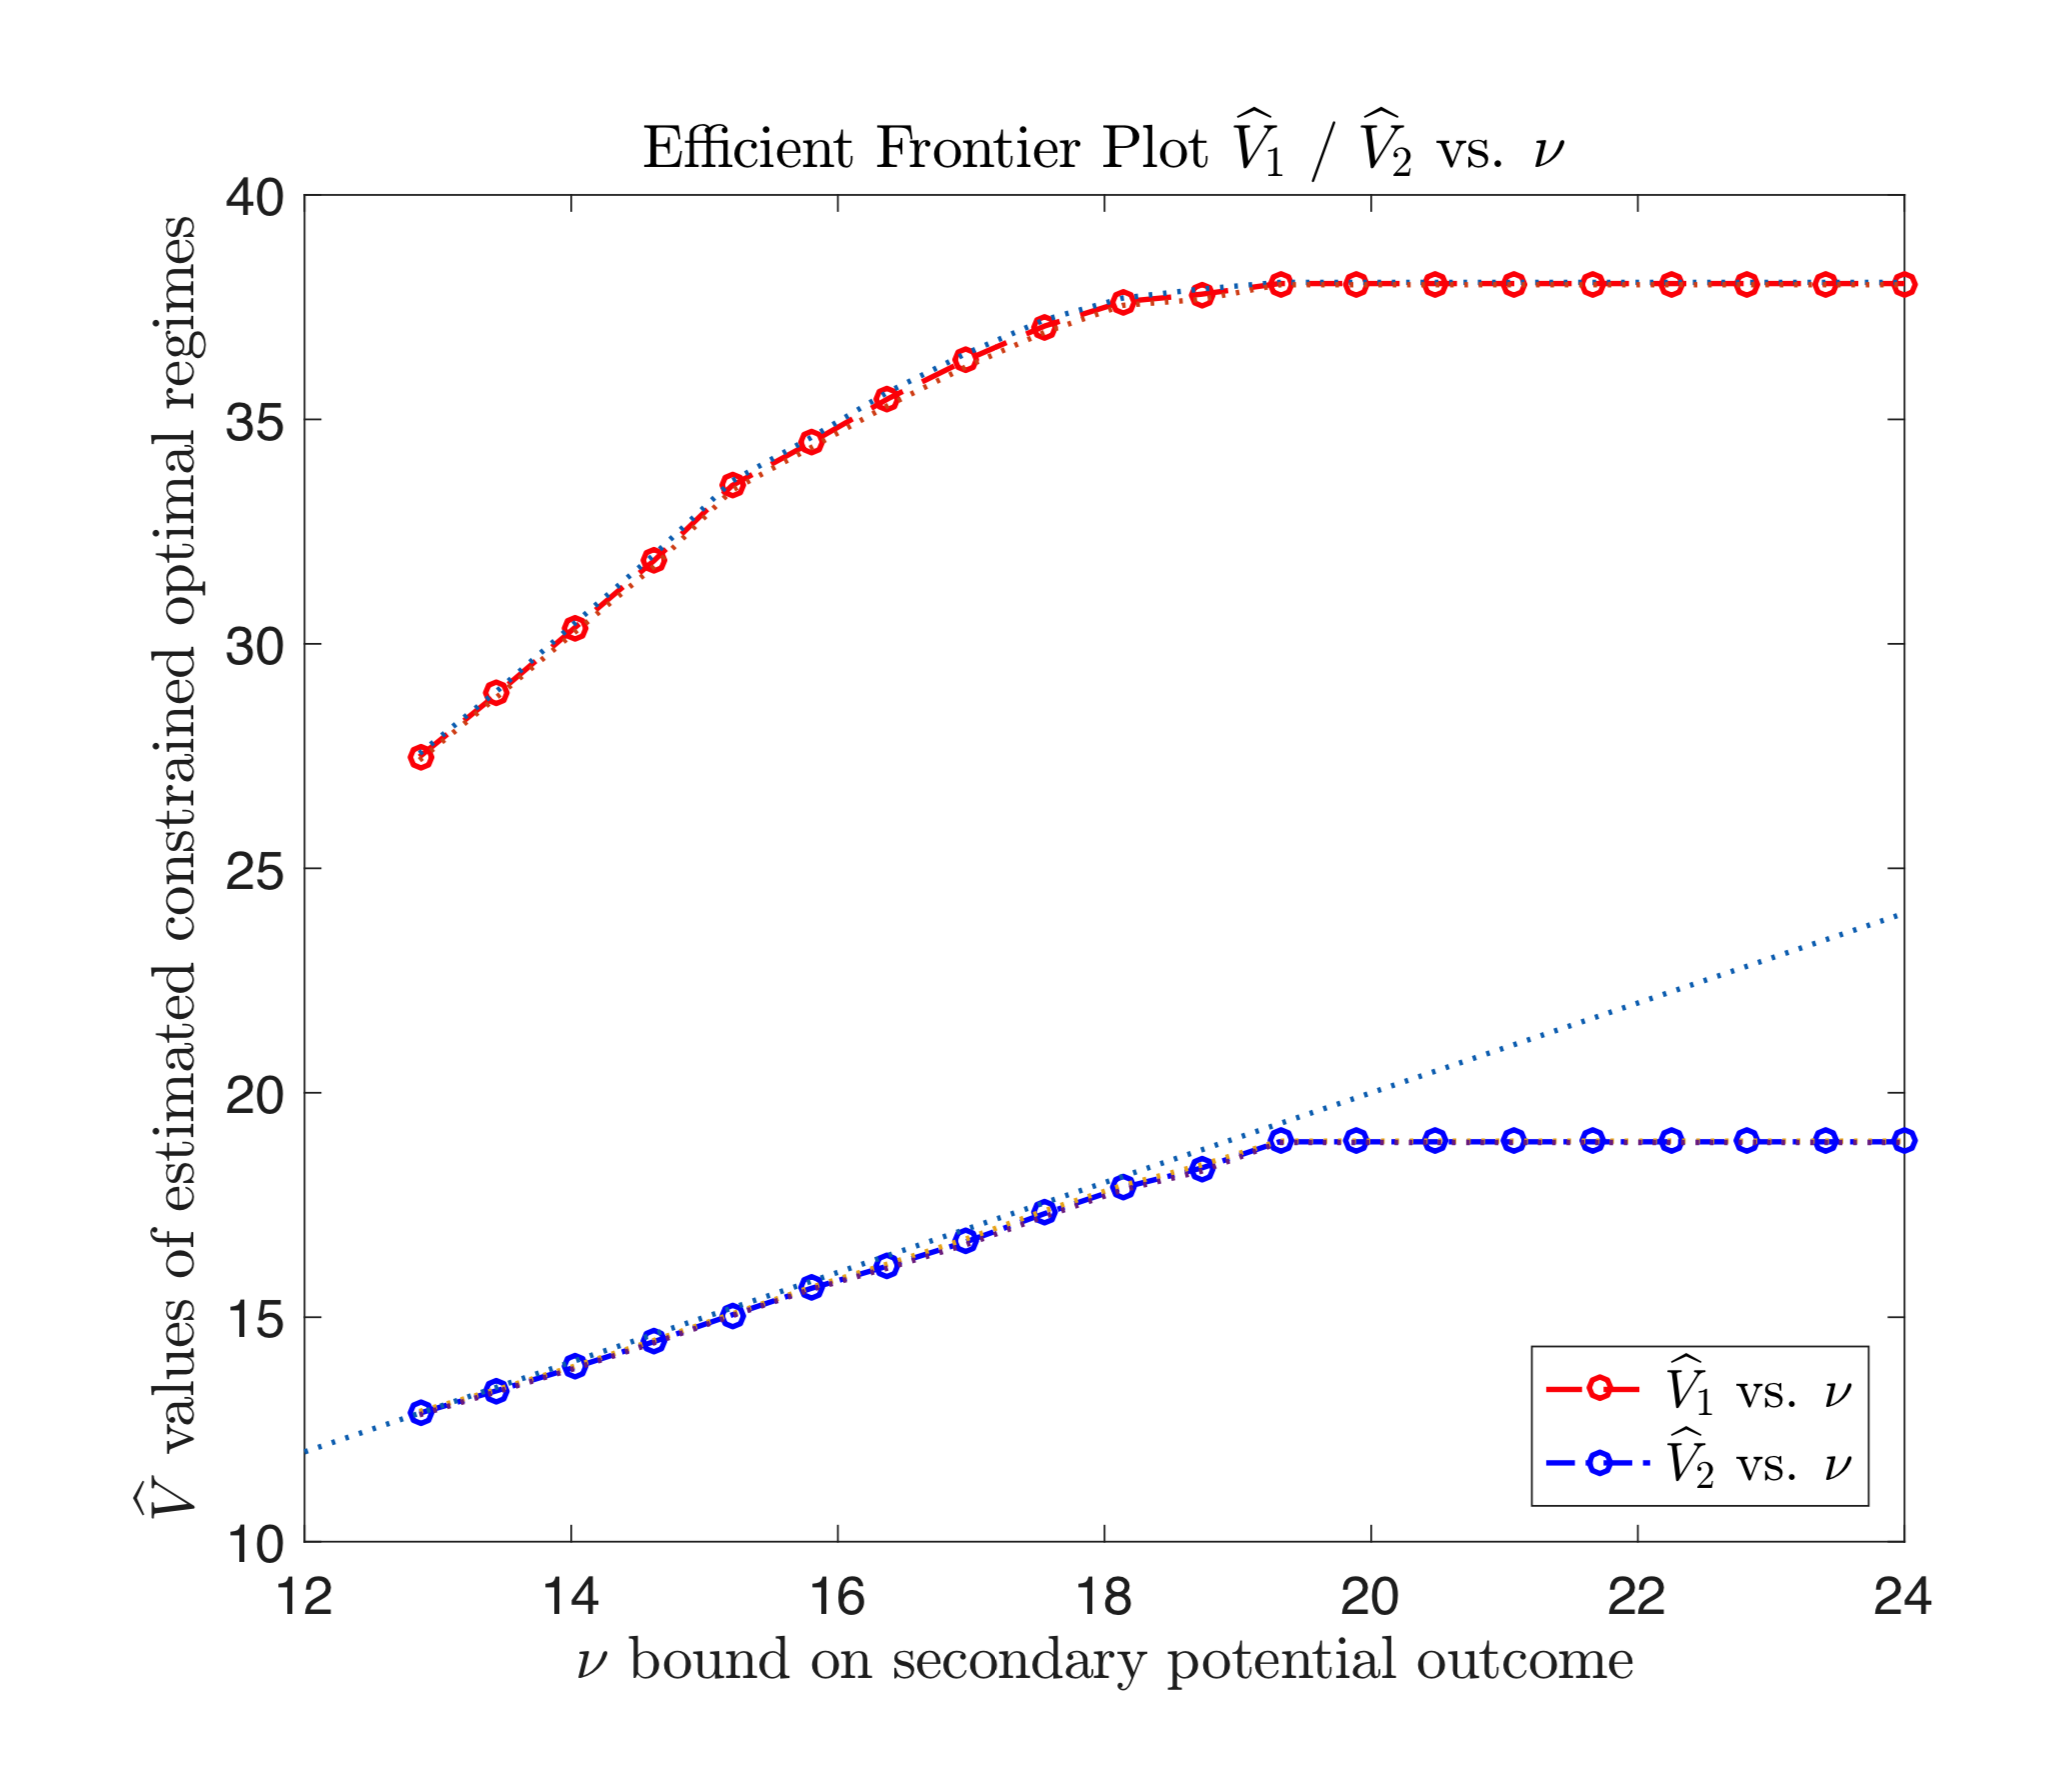
\includegraphics[width=0.9\linewidth]{./Chapter-2/figs/efficient_plot.png}
\caption{Efficient frontier for estimated constrained optimal regimes (multi-stage)}
\justify
X-axis is for the values for the constraints $\nu$; Y-axis is for the values of estimated regimes. Red dashed line is for the values in terms of the primary outcome of interest. Blue dashed line is for the values in terms of the secondary outcome of interest.
\end{figure}


\section{Conclusion}
Focusing on optimizing a single scalar outcome may be an oversimplification of the goals of practical clinical decision making. In this chapter, a new method is proposed to handle multiple competing outcomes in the multi-stage setting. Estimating an optimal treatment regime with competing outcomes is cast as a constrained optimization problem. We maximize the primary outcome of interest, subject to the constraints on the secondary outcomes of interest. Our estimator of a constrained optimal treatment regime has the properties of consistency and asymptotic normality under mild regularity conditions. The efficient frontier plots provide an intuitive visualization for clinicians to examine the trade-off between two competing outcomes. 

\chapter{Infinite-stage Constrained Optimal Treatment Regimes}
\label{chap-four}
\section{Introduction}
Precision medicine aims to accommodate interventions to individual patient attributes. For chronic illnesses, such as cancer, diabetes and so on, clinicians often need to make sequences of treatment decisions based on the evolving status of the patient's condition. To personalize this multi-stage intervention process, researchers have been developing dynamic treatment regimes (DTRs) to inform clinicians of treatment decisions adaptively. DTRs are a sequential decision making process, of which each decision is made based on the evolving patient status with the goal of maximizing the overall long-term treatment efficacy. It is well-studied in the statistical and biomedical literature ~\cite{Murphy2003, Moodie2004,Murphy2005,Zhang2012, Laber2014,Linn2014}. From the standpoint of Markov decision process, reinforcement learning algorithms, such as Q-learning~\cite{Murphy2005}, A-learning~\cite{blatt2004learning}, V-learning~\cite{Luckett2016} etc., are developed to estimate optimal treatment regimes. \\

Most previous methods for construct optimal dynamic treatment regimes have focused on optimizing a scalar measurement of the long-term efficacy over a fixed time period (finite stage).  However, in practice, the clinical situations are more complex. First, they often require consideration of the trade-off among multiple objectives, e.g., effectiveness, side-effect, cost, and so on. The preference of those objectives varies among people and changes over time, thus a single scalar reward or value can not represent the quality of a policy well enough. Thus, considering multiple rewards are necessary. Previous works by Lizotte et al. learn the value function and optimal policy for all preferences, i.e., all the possible convex combination of all the rewards~\cite{Lizotte2010,Lizotte2012}. More recent works adopt multi-objective Markov decision processes (MOMDPs) framework with finite stage. Practical domination is proposed for flexibility based on Pareto domination, and a set of policies that are maximal based on the partial order are treated as indistinguishably optimal~\cite{LaberTwo2014, Lizotte2016}. Secondly, patients with chronic diseases are often monitored and treated throughout their life. It often requires taking real-time actions and has no a-priori fixed end point (infinite stage), and progress is made in infinite stage reinforcement learning for health applications~\cite{Ertefaie2014,Murphy2016,Luckett2016}.\\

To deal with the trade-off between multiple objectives, we take a different perspective and adopt the constrained Markov decision processes (CMDPs) framework with infinite horizon. CMDPs are a well-studied framework for reinforcement learning under constraints~\cite{altman99cmdp}. The goal is to find the optimal policy, while satisfying constraints on expectations of secondary costs. For many applications of reinforcement learning, the constrained approach is more intuitive and more practical than eliciting a single reward function in order to achieve desirable results. For instance, satisfying safety constraints is necessary for systems that physically interact with humans. Previously, linear programming is used to seek constrained optimal policies in the setting of finite CMDPs with known models. However, few methods have been proposed for high-dimensional constrained reinforcement learning problems without modeling the underlying dynamics. Recently, Achiam et al~\cite{Achiam2017} proposed constrained policy optimization, a general-purpose policy search algorithm for constrained reinforcement learning guaranteeing near-constraint satisfaction at each iteration. Taking into consideration properties of clinical applications, such as data scarcity and off-policy learning, we develop an algorithm by taking advantage of least-squares policy evaluation and interior-point methods for estimating constrained optimal dynamic treatment regimes. Our method is applied to a simulated cancer trial dataset based on a chemotherapy mathematical model.\\

\section{Methodology}
\subsection{Set-up}
\subsubsection*{Observed Data}
We use dataset observed over a finite length of time steps to construct a regime in the setting of infinite horizon Markov decision process. The structure of the available data is  $\bs{D} = \lt\{  (\bs{S}^i_{0}, A^i_{0}, \bs{R}^i_{0} , \bs{S}^i_{1}, \cdots, 
\bs{S}^i_{T_i-1} , A^i_{T_i-1}, \bs{R}^i_{T_i-1}, \bs{S}^i_{T_i}) \rt\}_{i=1}^n,$
a set of $n$ independent, identically distributed trajectories of
$\lt(\bs{S}_{0}, A_{0}, \bs{R}_{0} , \bs{S}_{1}, \cdots, 
\bs{S}_{T-1} , A_{T-1}, \bs{R}_{T-1}, \bs{S}_{T}\rt).$
Note $T \in \mb{N}$ denotes the total number of follow-up time steps for a patient. For each patient, his or her follow up time length $T_i$ may be different. $\bs{S}_{t} \in \bs{\ml{S}}$ denotes a vector of patient clinical information recorded up to and including time point $t$, referred as \textit{state} in the reinforcement learning vocabulary. $\bs{\ml{S}} \subseteq \mb{R}^m$ denotes the support for state variable. Adopting the time homogeneous Markov decision process model, we assume $\bs{\ml{S}}$ is the same across all time points $t$.  $A_{t} \in \ml{A}$ denotes the treatment assignment at time point $t$ after measuring $\bs{S}_{t},$  referred as \textit{action} in reinforcement learning.  $\ml{A}$ denotes the support for treatment assignment, a finite set of all possible treatment options, and is assumed to be the same across all time points $t$. $\bs{R}_{t} \in \mb{R}^J$ is the reward obtained after treatment $A_{t}$ is assigned. We assume the reward, possibly defined based on domain expertise, is a known vector-valued function $\bs{r}$: $\bs{\ml{S}} \times \ml{A}  \times \bs{\ml{S}} \to \mb{R}^J $, so that $\bs{R}_{t} = \bs{r}(\bs{S}_{t}, A_t, \bs{S}_{t+1})$. The vector-valued reward function is the same across all the time points $t$ as well. Moreover, if a patient dies during the follow-up, say at decision point $t$, we set $\bs{S}_t = \bs{\emptyset}$, referred to as the absorbing state in reinforcement learning. Then, the patient's treatment assignment at time $t$ is $A_t=\emptyset$, and his/er length of follow-up $T = t$.	
\subsubsection*{Potential outcomes}
In reality, a patient can only be assigned to one of the sequences of treatment assignments. Hence, we can only observe the consequence of that treatment sequence, while the others remain unobserved. To identify the average causal effect of a certain regime, we adopt the counter-factual or potential outcomes framework,  established by Neyman, Rubin and Robins for assessment of the time-dependent treatment effect from either randomized or observational studies~\cite{Neyman,Robins1997,Rubin1980}. Let $\br{\bs{a}}_{t} = (a_0, a_1, \cdots, a_t) \in \br{\bs{\ml{A}}}_{t}$ be a possible treatment assignment sequence up to time point $t$, $t \ge 0$, where $\br{\bs{\ml{A}}}_t = \ml{A} \times \cdots \times \ml{A}$ is the set of all possible the treatment assignment sequences up to time point $t$. Let $\br{\bs{s}}_{t} = (\bs{s}_0, \bs{s}_1, \cdots, \bs{s}_t) \in \br{\bs{\ml{S}}}_{t}$ be a possible state sequences up to time point $t$, $t \ge 0$, where $\br{\bs{\ml{S}}}_t = \bs{\ml{S}} \times \cdots \times \bs{\ml{S}} $ is the set of all possible state sequences up to time point $t$. The set of potential outcomes is $\bs{W}^* = \lt\{\bs{S}^*_1(a_0), \bs{S}^*_2(\br{\bs{a}}_1),\cdots,  \bs{S}^*_{t+1}(\br{\bs{a}}_{t}), \cdots, \text{ for all } \br{\bs{a}}_{\infty} \in \br{\bs{\ml{A}}}_{\infty} \rt\}$, where $\bs{S}^*_{t+1}(\br{\bs{a}}_{t})$ is the potential state at $(t+1)$-th time point that would have been observed if the individual had been assigned the treatment sequence $\br{\bs{a}}_{t}$, $t \ge 0$. Moreover, if $\bs{S}_{t+1}^*(\br{\bs{a}}_{t}) = \bs{\emptyset}$ happens at time point $t+1$, then $\bs{S}_{t+2}^*(\br{\bs{a}}_{t+1}) =\bs{S}_{t+3}^*(\br{\bs{a}}_{t+2}) = \cdots = \bs{\emptyset}$, which indicates the patient, if followed treatment assignment sequence $\br{\bs{a}}_t$, would have died at time point $t+1$ in the counter-factual world.  Rewards with respect to potential states are $\bs{R}^*_t = \bs{r}(\bs{S}^*_t, A_t, \bs{S}^*_{t+1})$. The following assumptions are made in the potential outcome framework~\cite{Neyman, Rubin2005, Rubin1980, Robins1997, Hernan2006}.
\begin{itemize}
	\item  \textit{A1}. \textit{Consistency}:  $\bs{S}_{t+1} = \bs{S}^*_{t+1}(\br{\bs{A}}_{t})$, for all $t \ge 0$.
	\item \textit{A2}.  \textit{Sequential randomization assumption}: $A_{t+1} \indep \bs{W}^* \mid \br{\bs{S}}_{t+1}, \br{\bs{A}}_{t}$, for all $t \ge 0$.
	\item \textit{A3}. \textit{Positivity}: there exists $\epsilon_0 > 0$, so that $P\lt( A_{t+1} = a_{t+1} \mid \br{\bs{S}}_{t+1} = \br{\bs{s}}_{t+1}, \br{\bs{A}}_{t} = \br{\bs{a}}_{t} \rt) > \epsilon_0$, for all $a_{t+1} \in \mathcal{A}$, $\br{\bs{a}}_{t} \in \br{\bs{\ml{A}}}_t$ and $\br{\bs{s}}_{t+1} \in \br{\bs{\ml{S}}}_{t+1}$, and all $t \ge 0$.	 
\end{itemize}
These assumptions link the potential outcome and the observed data, and are guaranteed in well-designed Sequential, Multiple Assignment, Randomized Trials (SMARTs).  Therefore, the observed data from those trials are used to infer the average causal effect of a regime of interest.  

\subsubsection*{Markov Decision Processes}
To construct a regime in the infinite-horizon setting using a dataset observed over a finite number of time steps, we assume that the underlying dynamics is a time homogeneous Markov Decision Processes (MDPs). In infinite-horizon setting, MDP is considered as a 5-tuple of $(\bs{\ml{S}}, \ml{A}, \mb{P}, \bs{R}, \gamma)$, where $\bs{\ml{S}}$, $\ml{A}$ and $\bs{R}$ is as described above. Additionally, $\mb{P}$ is a markovian transition model in which $p(\bs{s}^{\prime} \mid \bs{s}, a)$ denotes the probability density of a transition to state $\bs{s}^{\prime}$ when taking action $a$ in state $\bs{s}$.  A discount factor for future reward, $\gamma \in [0, 1)$, is also introduced to form total discounted rewards, which are the value functions to operate constrained optimization on. The following assumptions are made for infinite-stage time homogeneous Markov decision process.
\begin{itemize}         
	\item \textit{A4}. \textit{Markov assumption}: $\bs{S}_{t+1} \indep \lt( \br{\bs{A}}_{t-1}, \br{\bs{S}}_{t-1} \rt) \mid \lt( A_{t}, \bs{S}_{t} \rt) $, for all $t \ge 1$.
	\item \textit{A5}. \textit{Time homogeneity}: the conditional density	$P_t(\bs{S}_{t+1} = \bs{s}^{\prime} \mid A_{t} = a, \bs{S}_{t} = \bs{s} ) = p(\bs{s}^{\prime} \mid a, \bs{s})$ for all $\bs{s} , \bs{s}^{\prime} \in \bs{\mathcal{S}}$ and $a \in \mathcal{A}$ and $t \ge 0$, where $\bs{s}$ and $\bs{s}^{\prime}$ denote the current state and the next state, respectively. 
\end{itemize}
As the time homogeneity is assumed in infinite-stage(3. setting, time step subscripts maybe dropped for simplicity.
\subsubsection*{Values of dynamic treatment regimes}
A dynamic treatment regime is equivalent to a \textit{policy} in reinforcement learning vocabulary, which is mostly to be considered deterministic. Thus, a dynamic treatment regime, $\pi : \bs{\ml{S}} \to \mathcal{A}$, is defined as a function which maps the support of the state variable to the set of the possible treatment assignments. As time homogeneity is assumed, we consider only stationary deterministic regimes, where this mapping function $\pi(\bs{s})$ does not change over time. Hence, a patient with state $\bs{S}_t = \bs{s}$ at time point $t$ will be assigned with treatment $A_t = \pi\lt(\bs{s}\rt)$ for all $t$.  
The value function $\bs{V}^{\pi}\lt(\bs{s}\rt)$ of a state under a certain policy $\pi$ is defined as the expected total discounted rewards when the process begins in state $\bs{s}$ and all decisions are made according to policy $\pi$. Mathematically, $\bs{V}^{\pi}\lt(\bs{s}\rt) = \mb{E}_{\bs{s}}^{\pi} \sum_{t=0}^{\infty} \gamma^{t} \, \bs{r}(\bs{s}_t, a_t, \bs{s}_{t+1})$, where $\mb{E}_{\bs{s}}^{\pi}$ is the expectation when the initial state is $\bs{s}$ and a policy $\pi$ is followed. The value function can also be defined recursively via the bellman equation, $\bs{V}^{\pi}\lt(\bs{s}\rt) = \sum_{\bs{s}^{\prime}\in\bs{\ml{S}}}  p(\bs{s}^{\prime} \mid \bs{s}, \pi(\bs{s})) \lt(\bs{R}(\bs{s}, \pi(\bs{s}), \bs{s}^{\prime}) + \gamma \bs{V}^{\pi}(\bs{s}^{\prime})\rt)$. Here, $\bs{V}^{\pi}(\bs{s}) \in \mb{R}^J$ has the same dimensionality as the reward vector $\bs{R}$, as we are considering multiple reward functions instead of a scalar reward function.  Moreover, the state-action value function under policy $\pi$, $\bs{Q}^{\pi}(\bs{s}, a) =\sum_{\bs{s}^{\prime} \in \bs{\ml{S}}}  p\lt(\bs{s}^{\prime} \mid \bs{s}, a\rt) \lt( \bs{R}\lt(\bs{s}, a, \bs{s}^{\prime}\rt) + \gamma \, \bs{Q}^{\pi}(\bs{s}^{\prime}, \pi(\bs{s}^{\prime}) ) \rt)$,
is defined similar but the first step takes action $a$ and $\bs{Q}^{\pi}(\bs{s}, a) \in \mb{R}^J$. In clinical cases, the transition model $\mb{P}$ is unknown, optimal regimes must be learn from observed dataset. In infinite horizon setting, as time steps are dropped, we break $n$ observed trajectories into 4-tuple of $(\bs{s}, a, \bs{r}, \bs{s}^{\prime})$ for estimating value functions. The counter-factual assumptions \textit{(A1-A3)} rule out the confounding phenomena and guarantee the identifiability of the average causal effect of a regime.
% Under these assumptions, the joint distribution of $S^{∗}_t(\pi)T$t=1 is non-parametrically identifiable under the data-generating model for any decision
%strategy $\pi$ and time horizon T.

\subsubsection*{Define infinite-stage constrained optimal dynamic treatment regimes}
Our strategy to cope with multiple competing outcomes is constrained optimization.  We optimize the primary outcome of interest, subject to the constraints on the secondary outcomes, over the space of all the possible regimes under consideration, $\Pi$. Here, the average of value functions is referred as competing outcomes, denoted as $\bs{V}(\pi) =\mb{E}\bs{V}^{\pi}(\bs{s}) $. The space of regimes under consideration may be crafted by experts with domain knowledge via policy function approximation. As We have $\bs{V}^{\pi}(\bs{s}) = \lt( V_1({\pi}), V^{\pi}_2(\bs{s}), \cdots, V^{\pi}_q(\bs{s})\rt)^\intercal$, Let $V_1(\pi) = \mb{E} V_1({\pi})$ be the primary outcome of interest, and $V_j(\pi) = \mb{E}V^{\pi}_j(\bs{s}), \, j = 2, 3, \cdots, J$ be the secondary outcomes. Mathematically, 
\begin{equation}
\begin{gathered}
\max_{\pi \in \Pi}  \,\, V_1(\pi), \\ 
\text{subject to}  \,\, V_j(\pi) \le \nu_{j-1},
\end{gathered}
\end{equation}
where $j = 2, \cdots, J$. The constraint upper-bounds $\bs{\nu} = (\nu_1, \nu_2, \cdots, \nu_{J-1})^\intercal$ can be specified based on patient preference and/or expert domain knowledge. Therefore, we define an infinite-stage  constrained optimal regime as $\pi^*_{\bs{\nu}} = \text{argmax}_{\pi \in \Pi} \,\, V_1({\pi})$, subject to $V_j(\pi) - \nu_{j-1} \le 0$, where $j = 2, \cdots, J$. Denote the feasible policy space, which is the set of all policy satisfying the constraints, as $\ml{F}(\Pi)$. For all $\pi \in \ml{F}(\Pi)$ and all $j = 2, \cdots, J$, $V_j({\pi}) \le \nu_{j-1}$. Then, an infinite-stage constrained optimal regime can also be written as $\pi^*_{\bs{\nu}} = \text{argmax}_{\pi \in \ml{F}(\Pi)}  V_1({\pi})$. To search over a feasible policy space with manageable computation complexity, we use policy function approximation such that $\pi(\bs{s})  = \pi(\bs{s}; \bs{\theta})$, where $\bs{\theta} \in \mb{R}^q$ is the indexing parameter for policies. Hence, we use $V_j(\pi)$ and $V_j(\bs{\theta})$ interchangeably, for all $j$. The search space is reduced from the set of all feasible policies to the feasible space of the indexing parameter $\bs{\theta} $, denoted as $\ml{F}(\bs{\Theta}) = \{ \bs{\theta} \in \mb{R}^q :  V_j(\bs{\theta}) \le \nu_{j-1},  j = 2, \cdots, J\}$.  \\

To carry out policy search, we need to solve the constrained optimization problem (3.1). This is done using interior-point methods, which are constrained nonlinear optimization methods for finding local optimums, implemented in Matlab fmincon \cite{Waltz2006,Byrd1999}.  We also need a method to estimate the value functions using observed dataset. This is done by least-square policy evaluation (LSQ) , a part of the least-squares policy iteration (LSPI) algorithm. \cite{Lagoudakis2003,Lagoudakis2001}. 

\subsection{Interior point method for constrained optimization}
To solve our constrained optimization problem (3.1) above, interior point algorithm is used. As the optimization softwares often implemented as minimization instead of maximization, we denote $v_1(\bs{\theta}) = - V_1\lt({\bs{\theta}}\rt)$ and  $v_j(\bs{\theta}) = V_j(\bs{\theta}) - \nu_{j-1}$, for $j = 2, \cdots, J$. Hence,  problem (3.1) notation is simplified as
\begin{equation}
\begin{gathered}
\min_{\bs{\theta} \in \bs{\Theta}}  \,\, v_1(\bs{\theta}) \\ 
\text{subject to}  \,\, v_j(\bs{\theta}) \le 0,
\end{gathered}
\end{equation}
where  $j = 2, \cdots, J$.
The interior point method solves a following sequence of approximate minimization problem (2), where $\rho$ is always positive and approaches to zero in the limit. For each $\rho >0$, the approximate problem is 
\begin{equation}
\begin{gathered}
\min_{\bs{\theta}, \bs{z}} \,\, f_{\rho}(\bs{\theta}, \bs{z}) = \min \,\,v_1(\bs{\theta}) - \rho \sum_{j=2}^J \ln(z_j), \text{ subject to } v_j(\bs{\theta})  + z_j = 0,
\end{gathered}
\end{equation}
where $j = 2, \cdots, J$. There are as many slack variables $z_j$ as there are inequality constraints $\nu_j$. The $z_j$ are restricted to be positive to keep $\ln(z_j)$ bounded. As $\rho$ decreases to zero, the minimum of $f_\rho$ should approach the minimum of $\nu_1$. The added logarithmic term is called a barrier function \cite{Waltz2006,Byrd1999}.
%\subsubsection{Definition of constrained optimal dynamic treatment regimes with infinite stages}
%Our strategy to cope with competing outcomes is constrained optimization, in which we optimize the primary outcome of interest, subject to the constraints on the secondary outcomes over the space of all the possible regimes under consideration, $\Pi$. Here, we refer the average of value functions as competing outcomes.  The space of regimes under consideration may be crafted by experts with domain knowledge via policy function approximation.  As $\bs{V}^{\pi}(\bs{s}) = (V^{\pi}_1(\bs{s}), V^{\pi}_2(\bs{s}), \cdots, V^{\pi}_q(\bs{s}))^\intercal$, we let $\mb{E}V^{\pi}_1(\bs{s})$ be the primary outcome of interest, and $\mb{E}V^{\pi}_j(\bs{s}), j = 2, 3, \cdots, J$ be the secondary outcomes. Mathematically, 
%\begin{equation}
%\begin{gathered}
%\max_{\pi \in \Pi}  \,\, \mb{E}V^{\pi}_1(\bs{s}) \\ 
%\text{subject to}  \,\, \mb{E}	V^{\pi}_j(\bs{s}) \le \nu_{j-1},
%\end{gathered}
%\end{equation}
%where $j = 2, \cdots, J$. The constraint upperbounds $\bs{\nu} = (\nu_1, \nu_2, \cdots, \nu_{J-1})^\intercal$ can be specified based on patient preference and/or expert domain knowledge. Therefore, we define the infinite-stage  constrained optimal regime as $\pi^*_{\bs{\nu}} = \text{argmax}_{\pi \in \Pi} \,\, \mb{E} V_1(\bs{s})$, subject to $\mb{E}	V_j(\bs{s}) - \nu_{j-1} \le 0$, where $j = 2, \cdots, J$. We denote the feasible policy space, which is the set of all policy satisfying the constraints, as $\ml{F}(\Pi)$. For all $\pi \in \ml{F}(\Pi)$ and all $j = 2, \cdots, J$, $\mb{E}V^{\pi}_j(\bs{s}) \le \nu_{j-1}$. Then, the infinite-stage constrained optimal regime can also be written as $\pi^*_{\bs{\nu}} = \text{argmax}_{\pi \in \ml{F}(\Pi)}\mb{E} V_1(\bs{s})$. \\
%
%To solve problem (1), we use a policy search in a certain feasible policy space combined with policy evaluation. To search over a feasible policy space with manageable computation complexity, we use policy function approximation such that $\pi(a \mid \bs{s}) = \pi(a \mid \bs{s}; \bs{\theta})$, where $\bs{\theta} \in \mb{R}^q$ is the indexing parameter for policies. Hence, we can use $\mb{E}V_j^{\pi}(\bs{s})$ and $V_j(\bs{\theta})$ interchangeably, for all $j$. Moreover, our search space is reduced from the set of all feasible policies to the feasible space of the indexing parameter $\bs{\theta} $, denoted as $\ml{F}(\Theta) = \{ \bs{\theta} \in \mb{R}^q : \mb{E} V^{\bs{\theta}}_j(\bs{s}) \le \nu_{j-1},  j = 2, \cdots, J\}$. To carry out policy search, we first need a method to estimate the value functions using observed dataset. This is done using least-square policy evaluation (LSQ / LSTDq) introduced in the LSPI paper [1,2]. Secondly, we need to solve the constrained optimization problem with the plugin-estimators of the value functions. This is done using interior-point method, which is a constrained nonlinear optimization method for finding local optimums, well implemented in Matlab fmincon. Both are described in the following.

\subsection{Least-squares policy evaluation}
 Least-squares policy evaluation, is adopted to approximate the state-action value function of a fixed regime/policy. As it is the state-action value function being approximated, instead of the state value function, changing policy is allowed without a model for the underlying dynamics. The exact $\bs{Q}^{\pi}$ values for all state-action pairs can be found by solving the linear system of the Bellman equations, $$\bs{Q}^{\pi}(\bs{s}, a) =\sum_{\bs{s}^{\prime} \in \ml{S}}  p(\bs{s}^{\prime} | \bs{s}, a) \lt\{ \bs{R}(\bs{s}, a, \bs{s}^{\prime}) + \gamma \sum_{a^{\p} \in \ml{A}} \pi(a^{\prime} \mid \bs{s}^{\p} ) \,\bs{Q}^{\pi}(\bs{s}^{\prime}, a^{\prime} ) \rt\},$$ for any $\bs{s} \in \ml{S}$ and $a^{\prime} \in \ml{A}$. Thus,  the state-action value function $\bs{Q}^{\pi}$ is considered the fixed point of the Bellman operator: $\bs{Q}^{\pi}=T^{\pi}\bs{Q}^{\pi}$, where the Bellman operator defined as \\  $T^{\pi}\bs{Q}^{\pi} =\sum_{\bs{s}^{\prime} \in \ml{S}}  p(\bs{s}^{\prime} | \bs{s}, a) \lt( \bs{R}(\bs{s}, a, \bs{s}^{\prime}) + \gamma \sum_{a^{\p} \in \ml{A}} \pi(a^{\prime} \mid \bs{s}^{\p} ) \,\bs{Q}^{\pi}(\bs{s}^{\prime}, a^{\prime} ) \rt)$.\\


Linear approximation is a  common way for estimating value functions, so that each component of the vector $\bs{Q}^{\pi}(\bs{s},a;w)$ are approximated by a linear parametric combination of $K$ basis functions (features). As $\bs{Q}(\bs{s},a) = (Q_1(\bs{s},a), Q_2(\bs{s},a), \cdots, Q_{J}(\bs{s},a))^{\intercal}$, the approximation for each component is $Q_j^{\pi}(\bs{s},a;w) = \sum_{k=1}^K \phi_{j,k}(\bs{s},a)w_{j,k} =  \bs{\phi}_{j}^{\intercal}(\bs{s}, a)\bs{w}_j$, where $\bs{w}_j = (w_{j,1}, \cdots, w_{j,K})^{\intercal}$ are the parameters to estimate. Moreover, the basis functions $\bs{\phi}_{j}(\bs{s}, a) = (\phi_{j,1}(\bs{s}, a), \cdots, \phi_{j,K}(\bs{s}, a))^{\intercal}$ are arbitrary and fixed, which are often non-linear functions of $\bs{s}$ and $a$ . It is also required that the basis functions $\phi_{j,k}$ are linearly independent to ensure that there are no redundant parameters and that the matrices involved in the computations are full rank. \\

Substituting each component of the Q function vector with the linear approximator, we get, for $j = 1, \cdots, J$,
%$$\wh{\bs{Q}}^{\pi}(\bs{s}, a) =\sum_{\bs{s}^{\prime} \in \bs{\ml{S}}}  p(\bs{s}^{\prime} | \bs{s}, a) \lt\{ \bs{R}(\bs{s}, a, \bs{s}^{\prime}) + \gamma \sum_{a^{\p} \in \ml{A}} \pi(a^{\prime} \mid \bs{s}^{\p} ) \,\wh{\bs{Q}}^{\pi}(\bs{s}^{\prime}, a^{\prime} ) \rt\}.$$ 
%For each component of $\bs{Q}^{\pi}(\bs{s}, a)$, we have 
%$$\wh{Q}_j^{\pi}(\bs{s}, a) =\sum_{\bs{s}^{\prime} \in \bs{\ml{S}}}  p(\bs{s}^{\prime} | \bs{s}, a) \lt\{ R_j(\bs{s}, a, \bs{s}^{\prime}) +  \gamma \sum_{a^{\p} \in \ml{A}} \pi(a^{\prime} \mid \bs{s}^{\p} ) \,\wh{Q}_j^{\pi}(\bs{s}^{\prime}, a^{\prime} )\rt\},$$ 
%for $j = 1, \cdot, J$
$$\bs{\phi}_j^\intercal(\bs{s},a)\bs{w}_j  =\sum_{\bs{s}^{\prime} \in \bs{\ml{S}}}  p(\bs{s}^{\prime} | \bs{s}, a)  R_j(\bs{s}, a, \bs{s}^{\prime}) + \gamma \sum_{\bs{s}^{\prime} \in \bs{\ml{S}}}  p(\bs{s}^{\prime} | \bs{s}, a)  \sum_{a^{\p} \in \ml{A}} \pi(a^{\prime} \mid \bs{s}^{\p} )  \bs{\phi}_j^\intercal(\bs{s}^{\prime}, a^{\prime})\bs{w}_j.$$
This fixed point equation then can be rearranged as
\begin{equation}
\begin{gathered}
 \lt\{\bs{\phi}_j^\intercal(\bs{s},a) - \gamma \sum_{\bs{s}^{\prime} \in \bs{\ml{S}}}  p(\bs{s}^{\prime} | \bs{s}, a)  \sum_{a^{\p} \in \ml{A}} \pi(a^{\prime} \mid \bs{s}^{\p} )  \bs{\phi}_j^\intercal(\bs{s}^{\prime}, a^{\prime})\rt\}\bs{w}_j =\sum_{\bs{s}^{\prime} \in \bs{\ml{S}}}  p(\bs{s}^{\prime} | \bs{s}, a) R_j(\bs{s}, a, \bs{s}^{\prime}).
 \end{gathered}
\end{equation}

Given a sample set of 4-tuples $\bs{\mathcal{D}} = \{\bs{s}^{i}, a^{i}, \bs{s}^{i\prime}, \bs{r}^i\}_{i=1}^N$, the equation (3.4) above becomes a over-constrained/overdetermined linear system over the parameter vector $\bs{w}_j$. The linear system can be written as
$$\bs{B}_j\bs{w}_j = \bs{b}_j,$$
where $\bs{B}_j = \bs{\Phi}_j^{\itl}(\bs{\Phi}_j - \gamma \bs{P}^{\pi}\bs{\Phi}_j )$ and $\bs{b}_j =\bs{\Phi}_j^{\intercal} \bs{R}_j$. Moreover,
$$\bs{\Phi}_j = \begin{pmatrix}
\bs{\phi}_j^\intercal(\bs{s}^1,a^1)  \\
\bs{\phi}_j^\intercal(\bs{s}^2,a^2) \\
\cdots\\
\bs{\phi}_j^\intercal(\bs{s}^n,a^n) \end{pmatrix}
\text{ , } 
\bs{P}^{\pi}\bs{\Phi}_j = \begin{pmatrix}
\sum_{\bs{s}^{\prime} \in \bs{\ml{S}}}  p(\bs{s}^{\prime} | \bs{s}^1, a^1)\bs{\phi}_j^\intercal(\bs{s}^{\prime},\pi(\bs{s}^{\prime})) \\
\sum_{\bs{s}^{\prime} \in \bs{\ml{S}}}  p(\bs{s}^{\prime} | \bs{s}^2, a^2)\bs{\phi}_j^\intercal(\bs{s}^{\prime},\pi(\bs{s}^{\prime})) \\
\cdots\\
\sum_{\bs{s}^{\prime} \in \bs{\ml{S}}}  p(\bs{s}^{\prime} | \bs{s}^n, a^n)\bs{\phi}_j^\intercal(\bs{s}^{\prime},\pi(\bs{s}^{\prime})) \end{pmatrix},$$
$$\text{and } \bs{R}_j=  \begin{pmatrix} \sum_{\bs{s}^{\prime} \in \bs{\ml{S}}}  p(\bs{s}^{\prime} | \bs{s}^1, a^1) R_j(\bs{s}^1, a^1, \bs{s}^{\prime}) \\
\sum_{\bs{s}^{\prime} \in \bs{\ml{S}}}  p(\bs{s}^{\prime} | \bs{s}^2, a^2) R_j(\bs{s}^2, a^2, \bs{s}^{\prime}) \\
\cdots \\
\sum_{\bs{s}^{\prime} \in \bs{\ml{S}}}  p(\bs{s}^{\prime} | \bs{s}^n, a^n) R_j(\bs{s}^n, a^n, \bs{s}^{\prime})\end{pmatrix},$$
where $\bs{\phi}_j^\intercal(\bs{s}^{\prime},\pi(\bs{s}^{\prime})) = \sum_{a^{\p} \in \ml{A}} \pi(a^{\prime} \mid \bs{s}^{\p} )  \bs{\phi}_j^\intercal(\bs{s}^{\prime}, a^{\prime}).$
Since the transition probability function $p(\bs{s}^{\prime} \mid \bs{s}, a)$ and reward functions $R_j(\bs{s}, a, \bs{s}^{\p})$ may be unknown,  we can construct approximators for $\bs{B}$ and $\bs{b}$ using samples. More precisely, we have approximated versions of $\bs{\Phi}_j$, $\bs{P}^{\pi}\bs{\Phi}_j$ and $\bs{R}_j$ based on the sample set as follows:
$$\wh{\bs{\Phi}}_j = \begin{pmatrix}
\bs{\phi}_j^\intercal(\bs{s}^1,a^1)  \\
\bs{\phi}_j^\intercal(\bs{s}^2,a^2) \\
\cdots\\
\bs{\phi}_j^\intercal(\bs{s}^n,a^n) \end{pmatrix}
\text{ , } 
\wh{\bs{P}^{\pi}\bs{\Phi}}_j = \begin{pmatrix}
\bs{\phi}_j^\intercal(\bs{s}^{1\prime},\pi(\bs{s}^{1\prime})) \\
\bs{\phi}_j^\intercal(\bs{s}^{2\prime},\pi(\bs{s}^{2\prime})) \\
\cdots\\
\bs{\phi}_j^\intercal(\bs{s}^{n\prime},\pi(\bs{s}^{n\prime})) \end{pmatrix} 
\text{ , and }
\wh{\bs{R}}_j=  \begin{pmatrix} r_1 \\
r_2 \\
\cdots \\
r_n\end{pmatrix}.$$
\\
Given $\wh{\bs{\Phi}}_j$, $\wh{\bs{P}^{\pi}\bs{\Phi}}_j$, and $\wh{\bs{R}}_j$, $\bs{B}_j$ and $\bs{b}_j$ can be approximated as
$\wh{\bs{B}}_j = n^{-1}\wh{\bs{\Phi}}_j^{\itl}(\wh{\bs{\Phi}}_j - \gamma \wh{\bs{P}^{\pi}\bs{\Phi}}_j ) =  n^{-1}\sum_{i =1}^n  \bs{\phi}_j(\bs{s}^i,a^i) \lt( \bs{\phi}_j(\bs{s}^i,a^i) - \gamma \bs{\phi}_j\lt(\bs{s}^{i\p},\pi\lt(\bs{s}^{i\p}\rt)\rt)\rt)$ and $\wh{\bs{b}}_j =n^{-1}\wh{\bs{\Phi}}_j^{\intercal} \wh{\bs{R}}_j= n^{-1}\sum_{i=1}^n \bs{\phi}_j(\bs{s}^i, a^i) r^i_j$. It is shown in the least-squares policy iteration paper that $\lim_{n \to \infty}\wh{\bs{B}}_j = \bs{B}_j$ and $\lim_{n \to \infty}\wh{\bs{b}}_j = \bs{b}_j$, if the samples are uniformly distributed over the state space. Moreover, the Markov property ensures that the solution $\wh{\bs{w}}^{\pi} = \wh{\bs{B}}^{-1}\wh{\bs{b}}$ will converge to the true solution $\bs{w}^{\pi}$ for sufficiently large $n$  whenever  $\bs{w}^{\pi}$  exists\cite{Lagoudakis2003,Lagoudakis2001}.The least-squares policy evaluation algorithm is listed in Algorithm 2 below.\\

Equipped with least-squares policy evaluation, we can hence calculate the values of any arbitrary regime/policy $\pi$. For $j = 1, \cdots, J$, $V\lt({\pi}\rt)$ is estimated by $n^{-1}\sum_{i=1}^{n} \wh{Q}^{\pi}_j(\bs{s}^i, \pi(\bs{s}^i)) = n^{-1}\sum_{i=1}^n\bs{\phi}_j^{\intercal}(\bs{s}^i,\pi(\bs{s}^{i}))\wh{\bs{w}}_j $.


%XXXXXXXXXXXXXXXXXXXXXXXXXXXXXXXXXXXXXXXXXXXXXXXXXXXXXXXXXXXX\\ Linear regression derivation review.
%least-squares policy evaluation step in LSPI: Least-Squares Fixed-Point Approximation
%
%1. Force the approximate Q function to be a fixed point under the Bellman operator: $T\widehat{Q}^{\pi} \approx  \widehat{Q}^{\pi}$.
%
%Bellman operator $T$: $TQ^{\pi}(s,a) = R(s,a) + \gamma \sum_{ s' \in \mathcal{S}} P(s,a,s')\sum_{ a' \in \mathcal{A}} \pi(a',s')Q(s',a')$. Bellman residual minimizing approximation is another choice.
%
%2. A sample $(s, a, r, s^{\prime})$ contributes to the approximation:
%$$\widehat{A} \leftarrow \widehat{A} + \phi(s,a)\{ \phi(s,a)^\intercal - \gamma\phi(s^{\prime},\pi(s^{\prime}))^\intercal \},$$
%$$\widehat{b} \leftarrow \widehat{b} + \phi(s,a)r$$
%3. Solve the linear system for $\omega^{\pi}$, 
%$$ A\omega^{\pi} = b$$

\subsubsection{Algorithm}
Putting together in the following box, our algorithm uses interior point method for policy search in terms policy indexing parameters $\bs{\theta}$, and least-squares policy evaluation for policy evaluation.\\
\begin{algorithm}[H]
	\caption{Constrained optimal regime with least-squares policy evaluation~\cite{Lagoudakis2003,Lagoudakis2001} for policy evaluation and interior-point method~\cite{Waltz2006,Byrd1999} for policy search.}
	\SetKwInOut{Input}{Input}
	\SetKwInOut{Output}{Output}
	\Input{A sample set $\bs{D}$ of 4 tuples $(\bs{s}^{\prime}, a, \bs{s}, \bs{r})$}
	\Output{Estimated constrained optimal regime $\wh{\pi}_{\bs{\nu}}$ indexed by $\wh{\bs{\theta}}_{\bs{\nu}}$}
	\BlankLine
	\BlankLine
	$\pi \leftarrow$  random initialization\\
	until converge\\
	\hspace{25pt} $\wh{\bs{Q}}^{\pi}(\bs{s}, a) \leftarrow$ least-squares policy evaluation $\lt(\bs{D}, \pi \rt)$\\
	\hspace{25pt} $\wh{\bs{V}}\lt(\pi\rt) \leftarrow \frac{1}{n}\sum_{i=1}^n\wh{\bs{Q}}^{\pi}(\bs{s}^i, \pi(\bs{s}^i))$\\
	\hspace{25pt} $\pi \leftarrow \underset{\pi \in \mathcal{F}(\Pi)}{\text{argmax }}	\bs{V}\lt({\pi}\rt)$\\
	end\\
	$\wh{\pi}_{\bs{\nu}} \leftarrow \pi$\\ 
	return $\wh{\pi}_{\bs{\nu}} $
\end{algorithm} 
\begin{algorithm}[H]
	\caption{Least-squares policy evaluation (LSQ).~\cite{Lagoudakis2003,Lagoudakis2001}}
	 \SetKwInOut{Input}{Input}
	\SetKwInOut{Output}{Output}
	\Input{A sample set $\bs{D}$ of 4 tuples $(\bs{s}^{\prime}, a, \bs{s}, \bs{r})$ \\
	$k$: Number of basis functions \\
	$\phi$: Basis functions \\
	$\gamma$: Discount factor \\
	$\pi$: policy whose value function is sought}
	\Output{Weights $\wh{\bs{w}}^{\pi}$}
	\BlankLine
	\BlankLine
	$\wh{\bs{B}} \leftarrow 0$ \hspace{25pt} // $(k\times k)$ matrix\\
	$\wh{\bs{b}} \leftarrow 0$ \hspace{28pt} // $(k\times 1)$ vector\\
	for each $(\bs{s}, a, \bs{r}, \bs{s}^{\prime}) \in \bs{D}$\\
	\hspace{25pt} $\wh{\bs{B}} \leftarrow \wh{\bs{B}} + \phi(\bs{s}, a)\lt(\phi(\bs{s}, a) - \gamma\phi(\bs{s}^{\prime}, \pi(\bs{s}^{\prime}))\rt)^{\intercal}$ \\
	\hspace{25pt} $\wh{\bs{b}} \leftarrow
	\wh{\bs{b}} + \phi(\bs{s}, a)\bs{r}$\\
	$\wh{\bs{w}}^{\pi} \leftarrow \wh{\bs{B}}^{-1}\wh{b}$\\
	return $\wh{\bs{w}}^{\pi}$
\end{algorithm} 

\section{Simulation}
\subsection{Chemotherapy mathematical model}
The chemotherapy mathematical model, a system of ordinary differential equations (ODE), proposed by Zhao et al \cite{odemodel}. is modified and used to generate a hypothetical clinical trial data. Their model reflects the capability of the drug to suppress tumor growth, as well as its negative impact on patient wellness due to the toxicity of chemotherapy. The dose assignment is discretized to $L=5$ levels, $\ml{A} = \left\{0.00, 0.25, 0.50, 0.75, 1.00 \right\}$.  Two state variables $W_t$ and $M_t$ are considered. $W_t$ denotes the patient negative wellness (toxcity) at time point $t$. $M_t$ denotes the tumor size observed at time point $t$. $A_t$ denotes chemotherapy agent dose at time point $t$. The ODE system is modeled as~\cite{odemodel}
$$\dot{W}_t = b_1 \max \,(M_t, M_0) + c_1 (A_t - d_1),$$
$$\dot{M}_t = \lt(b_2 \max \,(W_t, W_0) - c_2 (A_t - d_2)\rt) \times \mb{I} (M_t >0),$$
where decision points are $t= 0, 1,\cdots, T-1$. Moreover, $\dot{W}_t$ and $\dot{M}_t$ are the transition functions.  The indicator function term $\mb{I}(M_t > 0)$ means tumor size is absorbed at 0, the patient has been cured and no future tumor recurrence considered. These changing rate yields a piece-wise linear model over time.  Constants value are set as 
$b_1 = 0.1, b_2 = 0.15, c_1 = 1.2, c_2 = 1.2, d_1 = 0.5$ and $d_2 = 0.5$.  The initial states are draw as $M_0 \sim \text{Uniform}(0, 2)$ and $W_0 \sim \text{Uniform}(0, 2)$. The initial dose level assignment is draw as $A_0 \sim \text{Discrete Uniform} ( 0.25, 0.50, 0.75, 1.00 )$. The state variables for the next time point can be obtained via $W_{t+1} = \text{max } (W_t + \dot{W}_t, 0)$, $M_{t+1} = \text{max } (M_t + \dot{M}_t, 0)$.  The dose level assignment is drawn as
$A_t  \sim \text{Discrete Uniform} ( 0.00, 0.25, 0.50, 0.75, 1.00 )$, for $t = 1, \cdots, T-1$.\\

The survival status of the patient, denoted by $F_t$, is also modeled. We assume everyone is alive at the initial decision point $t=0$, that is $p_0 =0$ and $F_0 = 0$.  Death events occur during time interval $(t-1, t]$, $t = 1, 2, \cdots, 6$, and are recorded at the end of each interval as variable $F_t$, $t=1,2, \cdots, 6$. Assume that survival status depends on both toxicity and tumor size. For each time interval $(t-1, t]$, define the hazard function as $\lambda(t)$, where $\text{log } \lambda(t) = \mu_0 + \mu_1 W_t + \mu_2 M_t$, $\mu_1 = \mu_2 = 1$ and $\mu_0 = -8.5$. This again is a piece-wise linear approximation with $\lambda(t) = \text{exp}\lt( \mu_0 + \mu_1 W_t + \mu_2 M_t\rt)$. Then, the cumulative hazard function during time interval $(t-1, t]$ is
$\Delta \Lambda(t) = \sum_{t-1}^t \lambda(s) \,ds
= \sum_{t-1}^t \exp\lt( \mu_0 + \mu_1 W_t + \mu_2 M_t\rt) \,ds
=\exp\lt( \mu_0 + \mu_1 W_t + \mu_2 M_t\rt)$.  The survival function is $\Delta F(t) = \exp \lt( - \Delta \Lambda(t)\rt) = \exp \lt( - \exp\lt( \mu_0 + \mu_1 W_t + \mu_2 M_t\rt) \rt)$.
The random event of death during time interval $(t-1, t]$ is drawn as $F_t \sim \text{Bernoulli}(p_t) $, where \\
$p_t =1 - \text{exp}\lt( - \exp\lt( \mu_0 + \mu_1 W_t + \mu_2 M_t\rt) \rt)$.
If $F_{t-1} = 1$, then $F_t =1$. Also, as long as death occurred, all the other state variables at the following decision points are all set to null.\\

The reward functions here is a bivariate vector, consisting of positive reward and negative reward, denoted as $\boldsymbol{R}_t = ( R^+_t , R^-_t )^\intercal$. The positive reward function is used to assess tumor size reduction, while the negative reward to assess the increase of patient negative wellness (toxicity). Specifically, the reward functions are defined as follow. 
\begin{equation}
\begin{split}
R^{+}(:, t)  =  &  -15 \times \mb{I}( F_{ t+1} = 1) \\
& + 5 \times \mb{I}(  F_{ t+1 } \neq 1 , M_{ t+1} = 0 )   \\
&  + 5 \times \abs{ M_{t+1} - M_{t} } \times \mb{I}(  F_{ t+1} \neq 1, M_{ t+1 } - M_{t} <= 0  ) \\
& + 5 \times \abs{ M_{ t+1} - M_{t} } \times \mb{I}(  F_{ t+1 } \neq  1 , M_{t+1} - M_t \leq -0.5 ),
\end{split}
\end{equation}
\begin{equation}
\begin{split}
R^{-}_t = & 5 \times \abs{ W_{t+1} - W_{t} }  \times \mb{I} ( W_{t+1} - W_t) \ge -0.5 ) + \\
 & 5 \times \abs{ W_{ t+1} - W_{t} } \mb{I}( W_{t+1} - W_{t} \ge 0.5 ).
\end{split}
\end{equation}
To sum up, the trajectories / training data generated according to the ODE model, where with $N = 1000$ and $T = 6$, are as follow
$$\bs{S}_0 \overset{A_0}{\longrightarrow}\underset{\underset{\bs{R}_0}{\curvearrowright}}\, \bs{S}_1 \overset{A_1}{\longrightarrow} \underset{\underset{\bs{R}_1}{\curvearrowright}}\, \bs{S}_2 \overset{A_2}{\longrightarrow} \underset{\underset{\bs{R}_2}{\curvearrowright}}\,  \bs{S}_3 \overset{A_3}{\longrightarrow} \underset{\underset{\bs{R}_3}{\curvearrowright}}\,  \bs{S}_4 \overset{A_4}{\longrightarrow}  \underset{\underset{\bs{R}_4}{\curvearrowright}}\, \bs{S}_5 \overset{A_5}{\longrightarrow} \underset{\underset{\bs{R}_5}{\curvearrowright}}\,  \bs{S}_6, $$
where $\bs{S}_t = (M_t, W_t, F_t)$, $t = 0, 1, \cdots, 6$. Moreover, $\bs{R}_{t} = (R_t^+, R_t^-), t = 0, 1, \cdots, 5$. There are 7 decision points. The last decision point $T = 6$ has only states $\bs{S}_6 = (M_6, W_6, F_6)$, without following action nor reward. The trajectories is then broken down into 4-tuples of $(\bs{s}, a, \bs{s}^{\p}, \bs{r})$ with the time stamps dropped.
%The reward functions here is a bivariate vector, consisting of positive reward and negative reward, denoted as $\boldsymbol{R}_t = ( R^+_t , R^-_t )^\intercal$. The positive reward function is used to assess tumor size reduction, while the negative reward to assess the increase of patient negative wellness (toxicity). Specifically, the reward functions are defined as follow. \\
%\begin{minipage}{.5\linewidth}
%	\begin{flalign*}
%	R_t^+ & = \begin{cases}
%	0, & \text{ if } F_{t+1} = 1,\\
%	15 , & \text{ if } \,\, M_{t+1} = 0 \,\, \text{and} \,\,  F_{t+1} = 0, \\
%	5 , & \text{ if } \,\, M_{t+1} - M_t \le -0.5, \ M_{t+1} \ne 0 \,\, \text{and} \,\,  F_{t+1} = 0, \\
%	0 , & \text{  if } \,\, M_{t+1} - M_t > -0.5, \ M_{t+1} \ne 0 \,\, \text{and} \,\,  F_{t+1} = 0,
%	\end{cases}
%	\end{flalign*}
%\end{minipage}
%\begin{minipage}{.5\linewidth}
%	\begin{flalign*}
%	R_t^-  & = \begin{cases}
%	60, &  \text{ if } F_{t+1} = 1,\\
%	5 , & \text{ if } W_{t+1} - W_t \ge -0.5 \,\, \& \,\,  F_{t+1} = 0, \\
%	0 , & \text{ if }  W_{t+1} - W_t < -0.5 \,\, \& \,\,  F_{t+1} = 0. \\
%	\end{cases}
%	\end{flalign*}
%\end{minipage}

%The data generated according to the ODE model,  with sample size $N = 1000$ and lenght of time steps $T = 6$.
%, has the trajectory as 
%$$\bs{S}_0 \overset{A_0}{\longrightarrow}\underset{\underset{\bs{R}_0}{\curvearrowright}}\, \bs{S}_1 \overset{A_1}{\longrightarrow} \underset{\underset{\bs{R}_1}{\curvearrowright}}\, \bs{S}_2 \overset{A_2}{\longrightarrow} \underset{\underset{\bs{R}_2}{\curvearrowright}}\,  \bs{S}_3 \overset{A_3}{\longrightarrow} \underset{\underset{\bs{R}_3}{\curvearrowright}}\,  \bs{S}_4 \overset{A_4}{\longrightarrow}  \underset{\underset{\bs{R}_4}{\curvearrowright}}\, \bs{S}_5 \overset{A_5}{\longrightarrow} \underset{\underset{\bs{R}_5}{\curvearrowright}}\,  \bs{S}_6 $$
%where $\bs{S}_t = (M_t, W_t, F_t)$, and $\bs{R}_{t} = (R_t^+, R_t^-)$, for $t = 0, 1, \cdots, 5$. There are 7 decision points. The last decision point $T = 6$ has only states $\bs{S}_6 = (M_6, W_6, F_6)$, without action neither reward. The trajectories is then broken down into 4-tuples of $(\bs{s}, a, \bs{s}^{\p}, \bs{r})$ without worrying the time stamps.
\subsection{Function approximation}
\subsubsection{Q function approximation}
To construct linear approximators for Q functions~\cite{Geramifard2013}, we use $K=4$ Gaussian radial basis functions and an intercept of one. The Gaussian radial basis function has the form of $\phi(x) = \exp\lt(\sfrac{\| x - \mu\|^2}{2\sigma^2}\rt)$, where $\mu$ and $\sigma^2$ are the parameters to be specified.  %Specifically, a Gaussian basis function has the form of $\phi_{\cdot,\cdot}(x) = \exp\lt(\frac{\| x - \mu\|^2}{2\sigma^2}\rt) $ 
Denote the Q function for positive rewards as $Q^{+}(\bs{s}, a)$, and the one for negative rewards as  $Q^{-}(\bs{s}, a)$. %Their basis functions are denoted as $\phi^{+}_{\cdot, \cdot}(\cdot)$ and $\phi^{-}_{\cdot, \cdot}(\cdot)$, respectively.  
%We construct their linear approximators $\wh{Q}^{+}(\bs{s}, a)$ and $\wh{Q}^{-}(\bs{s}, a)$ using the same tactic but separately as described below.\\
As the positive reward function is a function of $M_t$, we only incorporate $M_t$ in the basis functions for estimating $Q^{+}(\bs{s}, a)$. Hence, we can rewrite $\wh{Q}^{+}(\bs{s}, a)$ as $\wh{Q}^{+}(m, a)$. Specifically, $\wh{Q}^{+}(m, a) = \wh{w}^{+}_0 + \sum_{k =1}^{4}\wh{w}^{+}_{k}\text{exp}\left( - \sfrac{\| m - \mu^{+}_k \|^2}{2(\sigma^{+}_k)^2} \right)$, where $\wh{w}^{+}_k$ are the weights to be estimated via least-squares policy evaluation. $\mu^{+}_{k}$'s are set as the 20, 40, 60, 80 percentiles of the states, and $\sigma^{+}_{k}$'s the average distance of the percentiles to all the sample points.  $\wh{Q}^-(\bs{s}, a)$ is constructed similarly.

\subsubsection*{Policy function approximation}
For policy function approximation~\cite{Geramifard2013}, we focus on simple decision rule to reduce the search space. Let $\bs{\theta} = (\theta_0, \theta_1, \theta_2, \theta_3, \theta_4, \theta_5)^{\itl}$ be the index parameters for a policy. The policy function is defined as $\pi(\bs{s}; \bs{\theta}) =  0.00 \times\mb{I}(f (\bs{s}, \bs{\theta} )  < 1 ) + 0.25 \times \mb{I}( 1 \le f (\bs{s}, \bs{\theta} )  < 2 ) +  0.50\times \mb{I}( 2 \le f (\bs{s}, \bs{\theta} ) < 3) + 0.75\times\mb{I}( 3 \le f( \bs{s}, \bs{\theta}) < 4) + 1\times \mb{I} ( f( \bs{s}, \bs{\theta}) > 4)$, where $f(\bs{s}, \bs{\theta} ) = \theta_0 + \theta_1  m + \theta_2  m^2 + \theta_3 w + \theta_4 w^2 + \theta_5  m  w $.

\subsection{Simulation results}
The goal here is to maximize $V^{+}(\pi)$, subject to  $V^{-}(\pi) \le \nu$, where $\nu$ is the bound on the secondary outcome. We applied our method to the simulated dataset. Table 3.1. shows the values of primary and secondary outcomes of the estimated constrained optimal regimes, along with their standard deviations. Table 3.2. shows the estimated indexing parameters of the estimated regimes, along with their standard deviations. Figure 3.1. shows the values of the primary objective(red) / secondary objective (blue) vs. constraint $\nu$. Figure 3.2-3.6 shows the actions of the estimated regime for each state under different constraint values. As the $\nu$ increases,  we start to observe more higher dosages being assigned to patients. Higer dosage leads to better treatment effect (more reduced tumor size), but more toxicity on patient's wellness. 

%\begin{table}[!htbp]
%	\centering
%	{\tt
%		\input{./result_tab.tex}
%	}
%	\caption {Simulation Results}
%\end{table} 
\begin{table}[!htbp]
\caption{Values of estimated optimal regimes under different constraint bounds.}
	\centering
\begin{tabular}{rrrrr}\hline 
	$\nu$  & $\widehat{V}^{+}$ & $std^{+}$ & $\widehat{V}^{-}$ & $std^{-}$ \\\hline 
	5.49 &     0.39 &     0.36 &     5.42  &     0.16 \\ 
	6.85 &     1.35 &     0.29 &     6.62  &     0.43 \\ 
	8.21 &     3.58 &     1.06 &     7.66  &     0.30 \\ 
	9.57 &     4.07 &     0.89 &     7.77  &     0.35 \\ 
	10.93 &     4.97 &     0.56 &     9.53  &     1.42 \\ 
	12.29 &     5.98 &     1.10 &    11.43  &     0.69 \\ 
	13.65 &     6.13 &     0.99 &    11.90  &     1.46 \\ 
	15.01 &     7.08 &     0.93 &    14.88  &     0.42 \\ 
	16.37 &     7.98 &     1.31 &    14.69  &     2.15 \\ 
	17.73 &     8.89 &     0.61 &    16.84  &     0.57 \\ 
	19.09 &     9.15 &     0.30 &    16.93  &     0.71 \\ 
	20.45 &     9.85 &     1.16 &    17.86  &     2.33 \\ 
	21.81 &     9.76 &     1.01 &    18.18  &     2.88 \\ 
	23.18 &     9.76 &     1.01 &    18.18  &     2.88 \\ 
	24.54 &    11.62 &     1.38 &    21.88  &     0.63 \\ 
	25.89 &    12.02 &     1.17 &    23.45  &     2.47 \\ 
	27.25 &    12.04 &     1.17 &    23.57  &     2.69 \\ 
	28.61 &    12.86 &     0.54 &    28.27  &     1.06 \\ 
	29.98 &    13.69 &     0.57 &    30.25  &     1.04 \\ 
	31.34 &    14.53 &     0.97 &    31.11  &     1.10 \\ \hline 
\end{tabular}
\caption*{The constraint bounds are denoted by $\nu$. $\wh{V}^{+}$ denotes the primary outcome values of the estimated regimes. $\wh{V}^{-}$ denotes the secondary outcome values of the estimated regimes. Standard deviations of those estimated regime values are reported as well.}
\end{table} 
\begin{table}[!htbp]
\caption{The estimated indexing parameters of estimated regimes under different constraint bounds.}
	\centering
\begin{tabular}{rrrrrrrrrrrrr}\hline 
	$\nu$ & $\widehat{\theta}_{\nu,1}$ & $std_1$ & $\widehat{\theta}_{\nu,2}$ & $std_2$ & $\widehat{\theta}_{\nu,3}$ & $std_3$ & $\widehat{\theta}_{\nu,4}$ & $std_4$ &  $\widehat{\theta}_{\nu,5}$ & $std_5$ & $\widehat{\theta}_{\nu,6}$ & $std_6$ \\ \hline 
	5.49 &     0.36 &     0.79 &    -0.38 &     0.76  &     0.13 &     0.48 &     0.03 &     0.84 &    -0.29 &     0.71  &    -0.06 &     0.76 \\ 
	6.85 &     0.11 &     1.47 &    -1.55 &     1.10  &     0.29 &     0.67 &     0.35 &     1.44 &    -1.06 &     1.19  &    -0.20 &     1.41 \\ 
	8.21 &    -0.00 &     1.66 &    -2.02 &     1.09  &     0.58 &     0.80 &     0.27 &     1.48 &    -1.26 &     1.40  &    -0.41 &     1.53 \\ 
	9.57 &     0.29 &     1.65 &    -2.38 &     1.16  &     0.58 &     0.84 &     0.32 &     1.71 &    -1.43 &     1.37  &     0.02 &     1.66 \\ 
	10.93 &     0.49 &     1.64 &    -2.61 &     1.13  &     0.67 &     0.90 &     0.18 &     1.72 &    -1.47 &     1.57  &     0.23 &     1.64 \\ 
	12.29 &     0.46 &     1.70 &    -2.90 &     1.16  &     0.71 &     0.89 &     0.08 &     1.90 &    -1.27 &     1.58  &     0.26 &     1.59 \\ 
	13.65 &     0.56 &     1.76 &    -3.20 &     1.12  &     0.70 &     0.92 &     0.01 &     1.70 &    -1.06 &     1.66  &     0.32 &     1.58 \\ 
	15.01 &     0.67 &     1.74 &    -3.46 &     1.08  &     0.65 &     0.90 &    -0.02 &     1.87 &    -0.83 &     1.77  &     0.14 &     1.55 \\ 
	16.37 &     0.89 &     1.81 &    -3.49 &     1.10  &     0.48 &     0.95 &    -0.05 &     1.95 &    -0.43 &     1.81  &     0.16 &     1.61 \\ 
	17.73 &     0.88 &     1.92 &    -3.54 &     1.17  &     0.39 &     0.99 &    -0.21 &     2.03 &    -0.07 &     1.70  &     0.05 &     1.56 \\ 
	19.09 &     1.20 &     2.08 &    -3.36 &     1.54  &     0.47 &     1.17 &    -0.41 &     2.14 &     0.11 &     1.56  &     0.15 &     1.52 \\ 
	20.45 &     1.69 &     2.18 &    -3.06 &     1.79  &     0.72 &     1.44 &    -0.84 &     2.28 &     0.13 &     1.52  &     0.16 &     1.61 \\ 
	21.81 &     1.95 &     2.20 &    -2.78 &     2.06  &     1.05 &     1.64 &    -0.88 &     2.40 &     0.12 &     1.48  &     0.27 &     1.88 \\ 
	23.18 &     2.21 &     2.21 &    -2.64 &     2.19  &     1.30 &     1.76 &    -1.09 &     2.32 &     0.15 &     1.47  &     0.03 &     1.93 \\ 
	24.54 &     2.46 &     2.27 &    -2.46 &     2.23  &     1.46 &     1.86 &    -1.32 &     2.31 &     0.36 &     1.43  &    -0.14 &     2.13 \\ 
	25.89 &     2.84 &     2.14 &    -2.14 &     2.32  &     1.70 &     2.03 &    -1.57 &     2.12 &     0.61 &     1.45  &    -0.19 &     2.31 \\ 
	27.25 &     3.25 &     1.82 &    -1.95 &     2.26  &     1.66 &     2.14 &    -1.60 &     2.05 &     1.01 &     1.60  &    -0.12 &     2.41 \\ 
	28.61 &     3.41 &     1.73 &    -1.86 &     2.26  &     1.58 &     2.08 &    -1.10 &     2.06 &     1.46 &     1.65  &    -0.05 &     2.53 \\ 
	29.98 &     3.65 &     1.42 &    -1.53 &     2.27  &     2.00 &     2.06 &    -0.98 &     2.04 &     1.99 &     1.68  &    -0.07 &     2.65 \\ 
	31.34 &     3.89 &     1.14 &    -1.07 &     2.18  &     2.23 &     1.91 &    -0.60 &     2.15 &     2.64 &     1.61  &    -0.13 &     2.70 \\ \hline 
\end{tabular}
\caption*{ Here, $\nu$ denotes the constraint bounds. $\wh{\theta}_{\nu,j}$ denotes the $j$-th component of the estimated parameter vector $\wh{\bs{\theta}}_{\nu}$ of the estimated regimes. Standard deviations of those estimated regime values are reported as well.}
\end{table} 
\begin{figure}[!htbp]
	\centering
	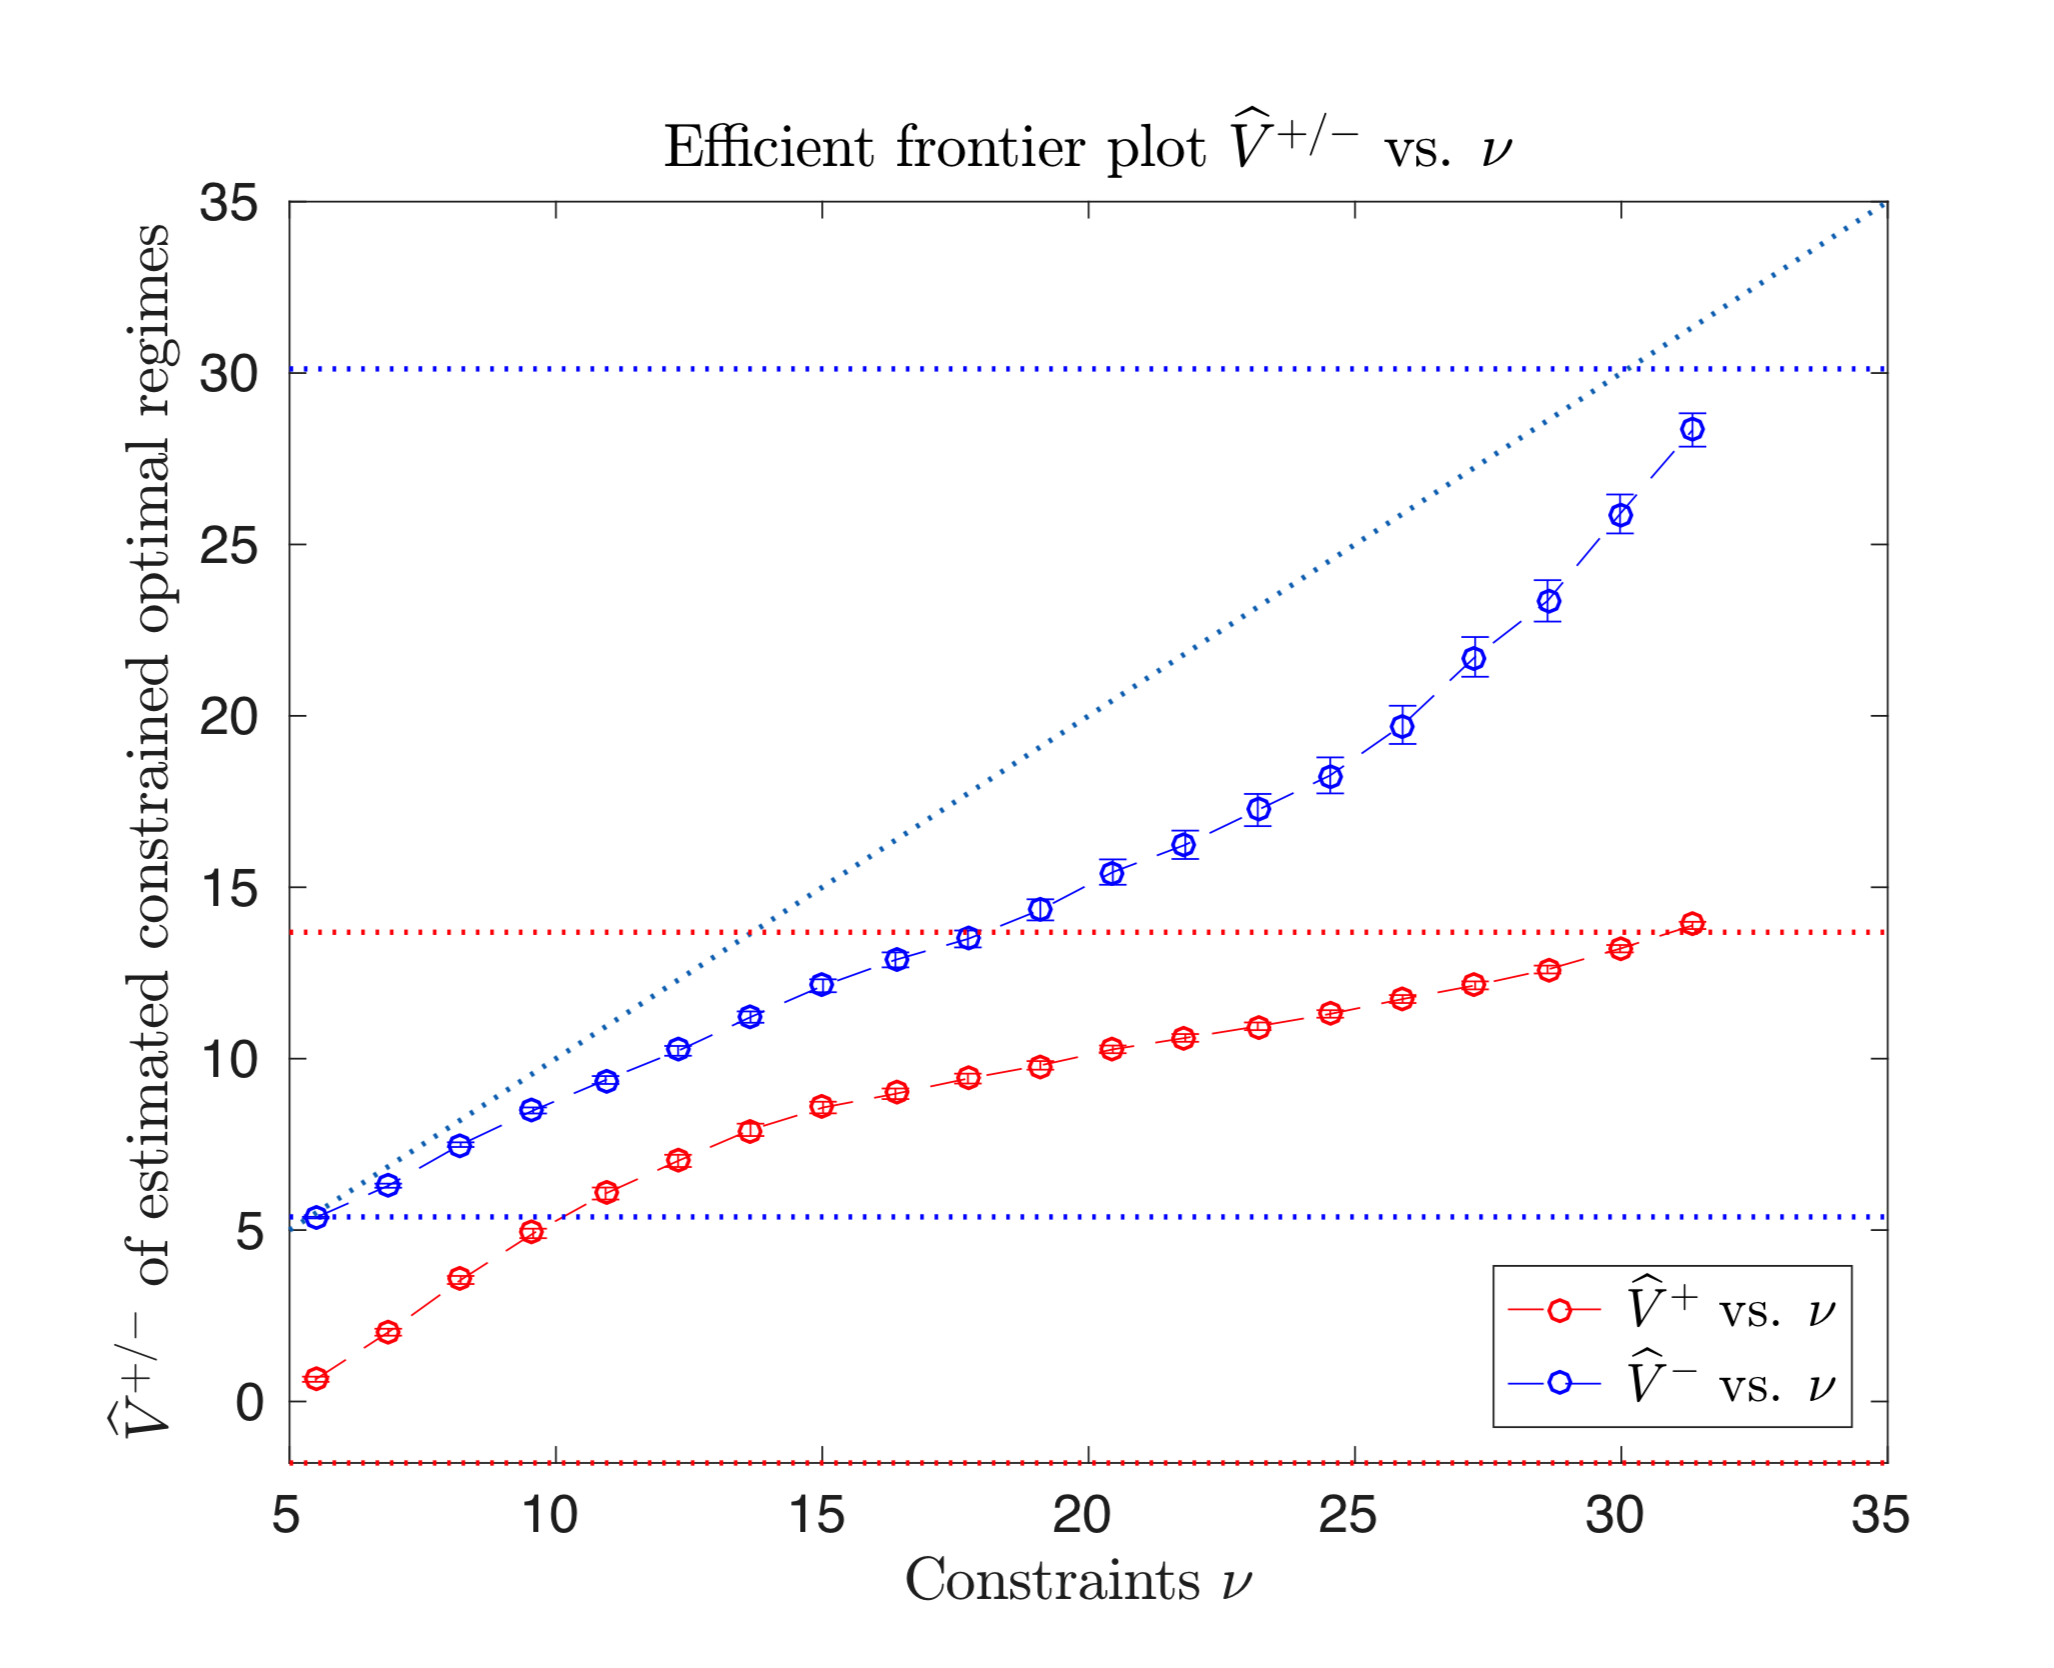
\includegraphics[width=.9\linewidth]{./Chapter-3/figs/efficient_plot.png}
	\caption{Efficient frontier for estimated constrained optimal regimes (infinite-stage).}
	\caption*{The red dashed line is for the primary outcome to maximized. The blue dashed line is for the secondary outcome to be constrained. The red dotted lines are the minima and maxima for unconstrained optimization of the primary objective. The blue dotted lines are the minimal and maximal for unconstrained optimization of the secondary objective.}
	\label{fig:1}
\end{figure}
%\begin{figure}[!htbp]
%	\centering
%	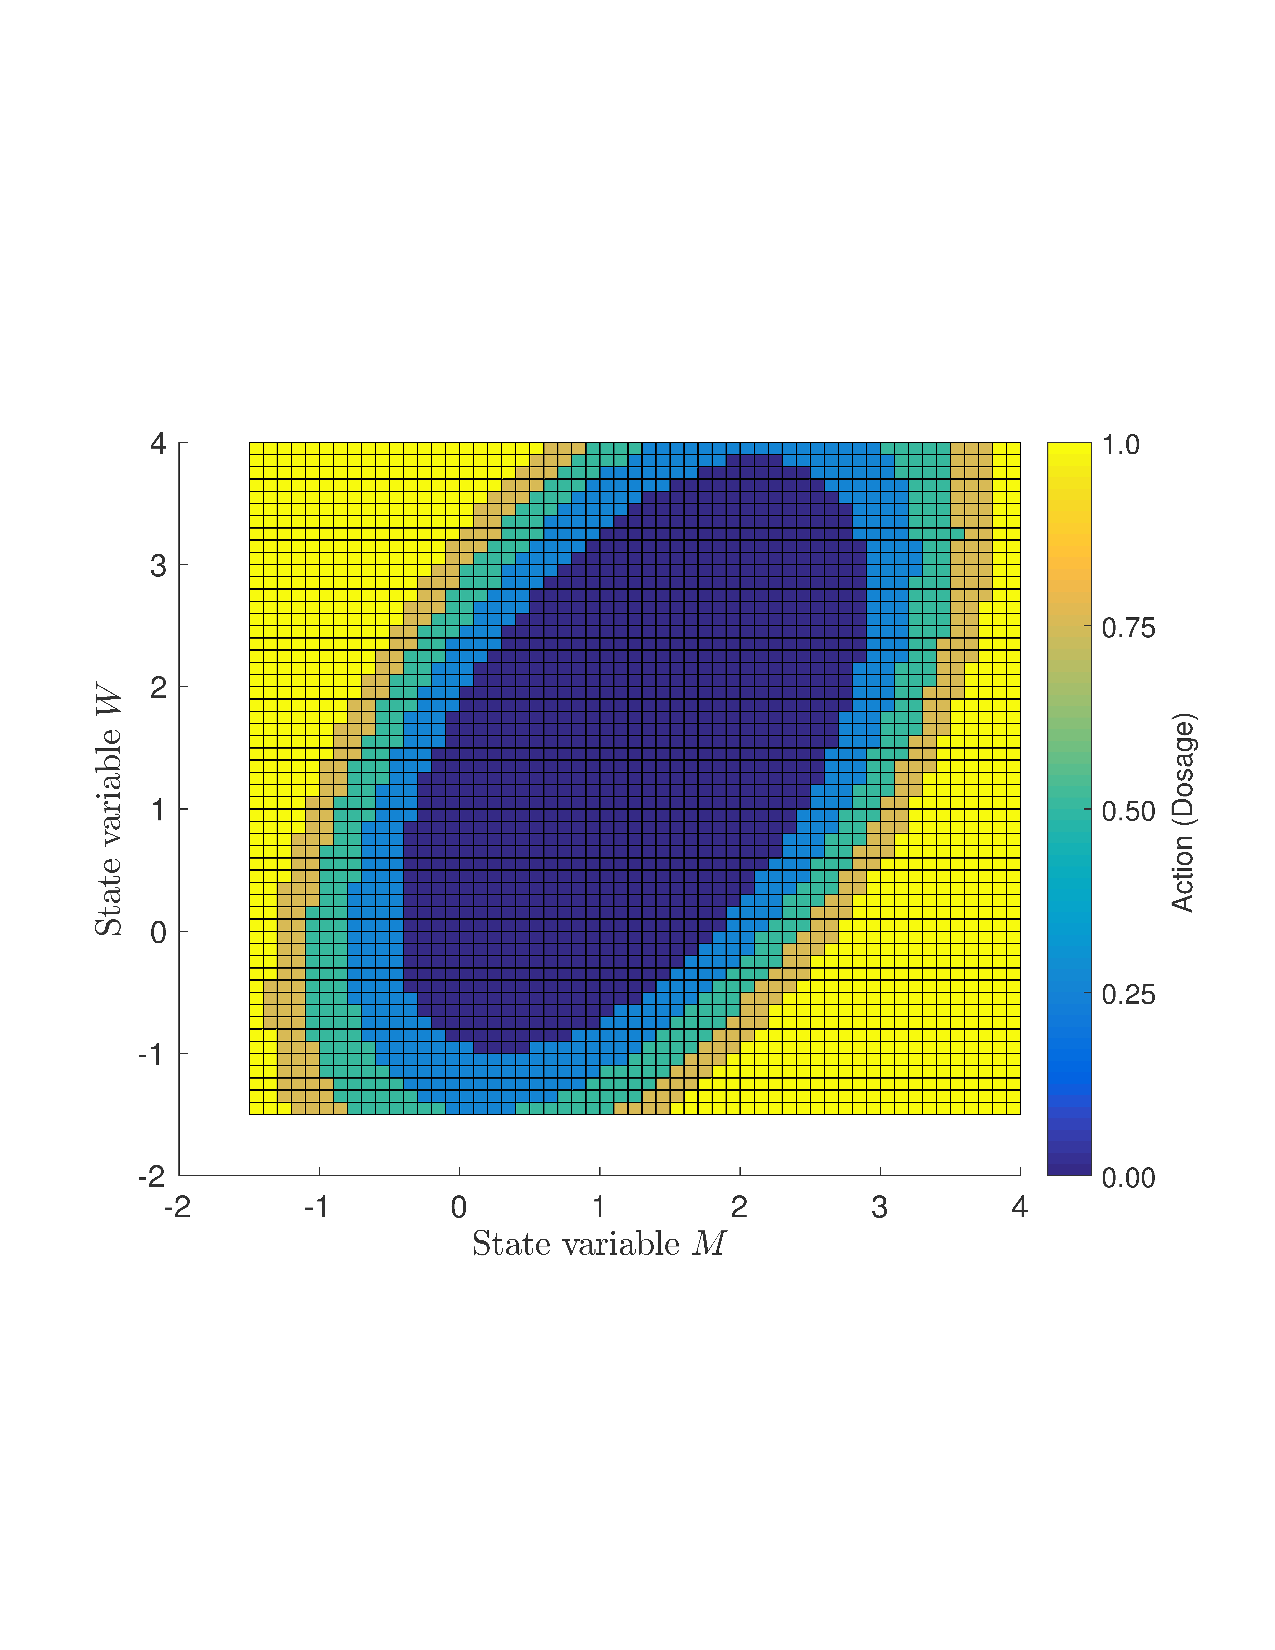
\includegraphics[width=.9\linewidth]{./Chapter-4/figs/action_nu5.pdf}
%	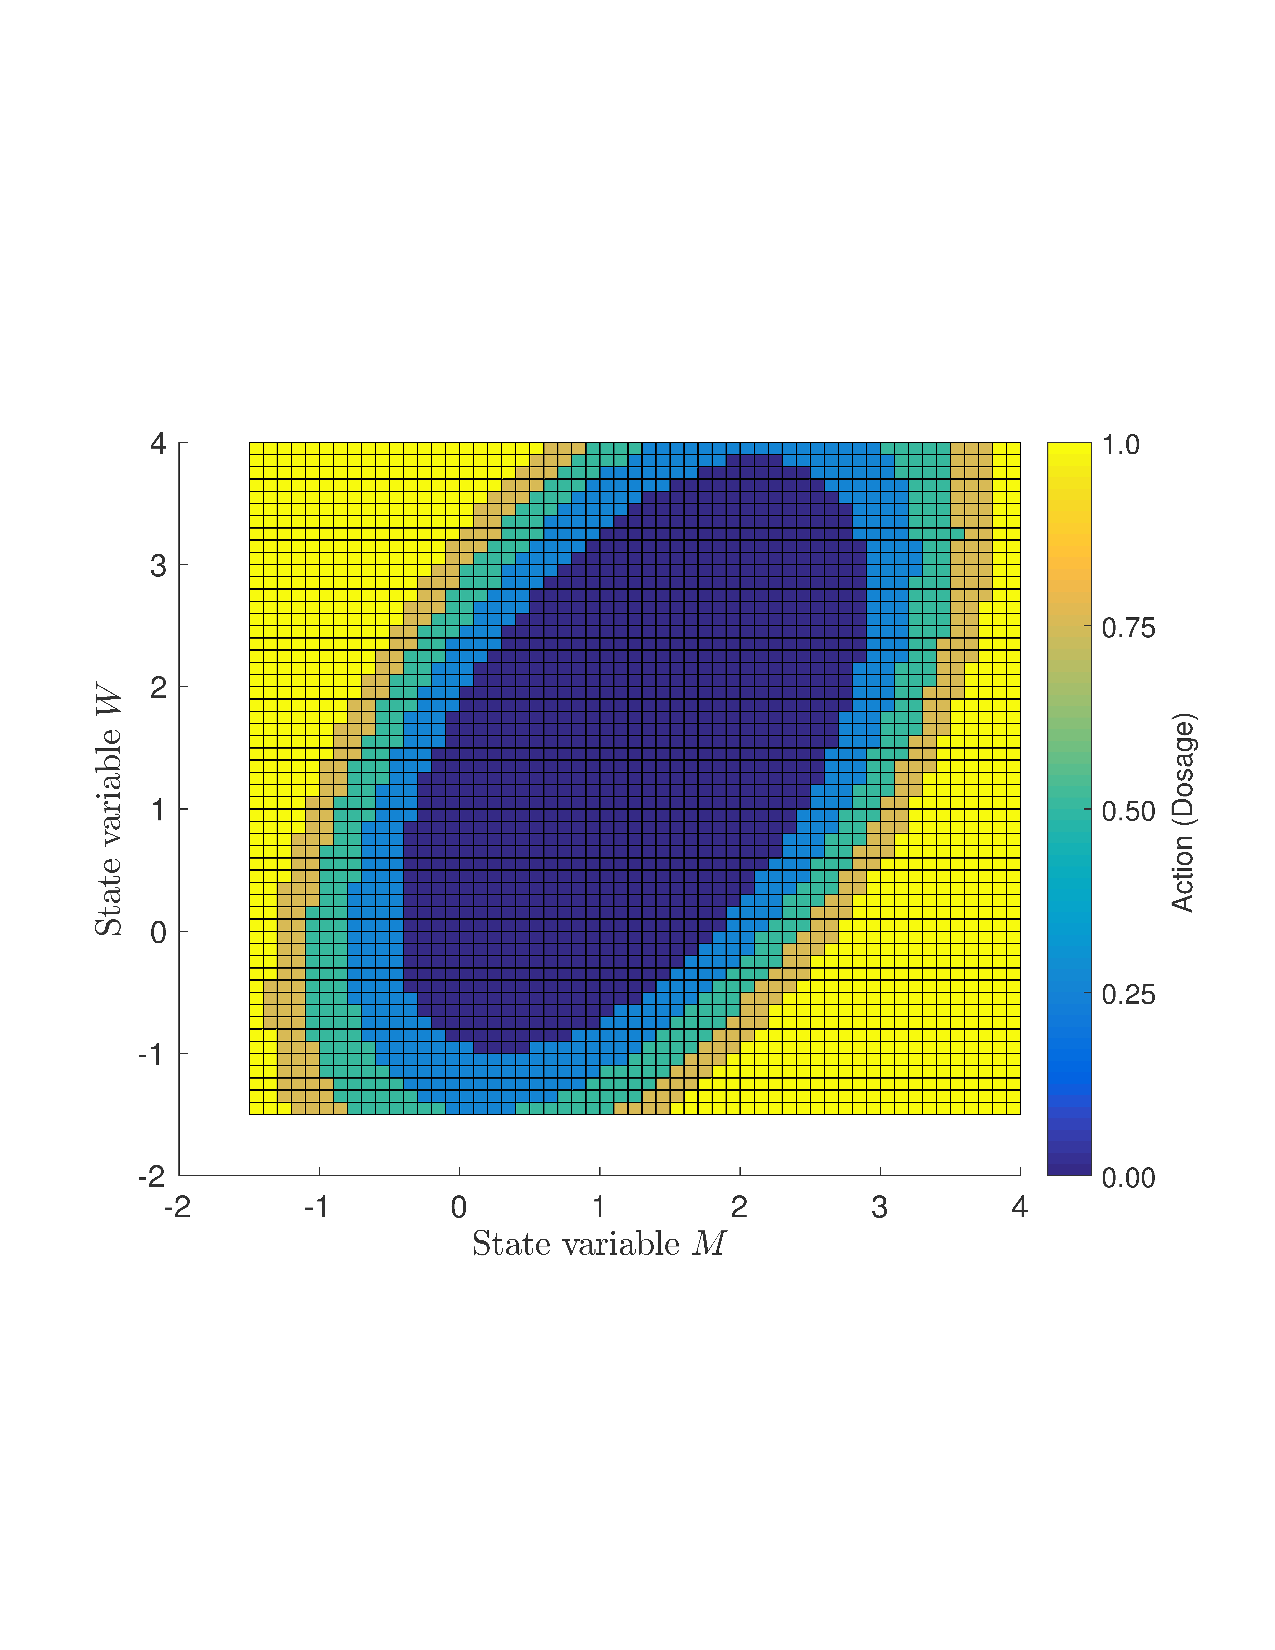
\includegraphics[width=.9\linewidth]{./Chapter-4/figs/action_nu5.pdf}
%	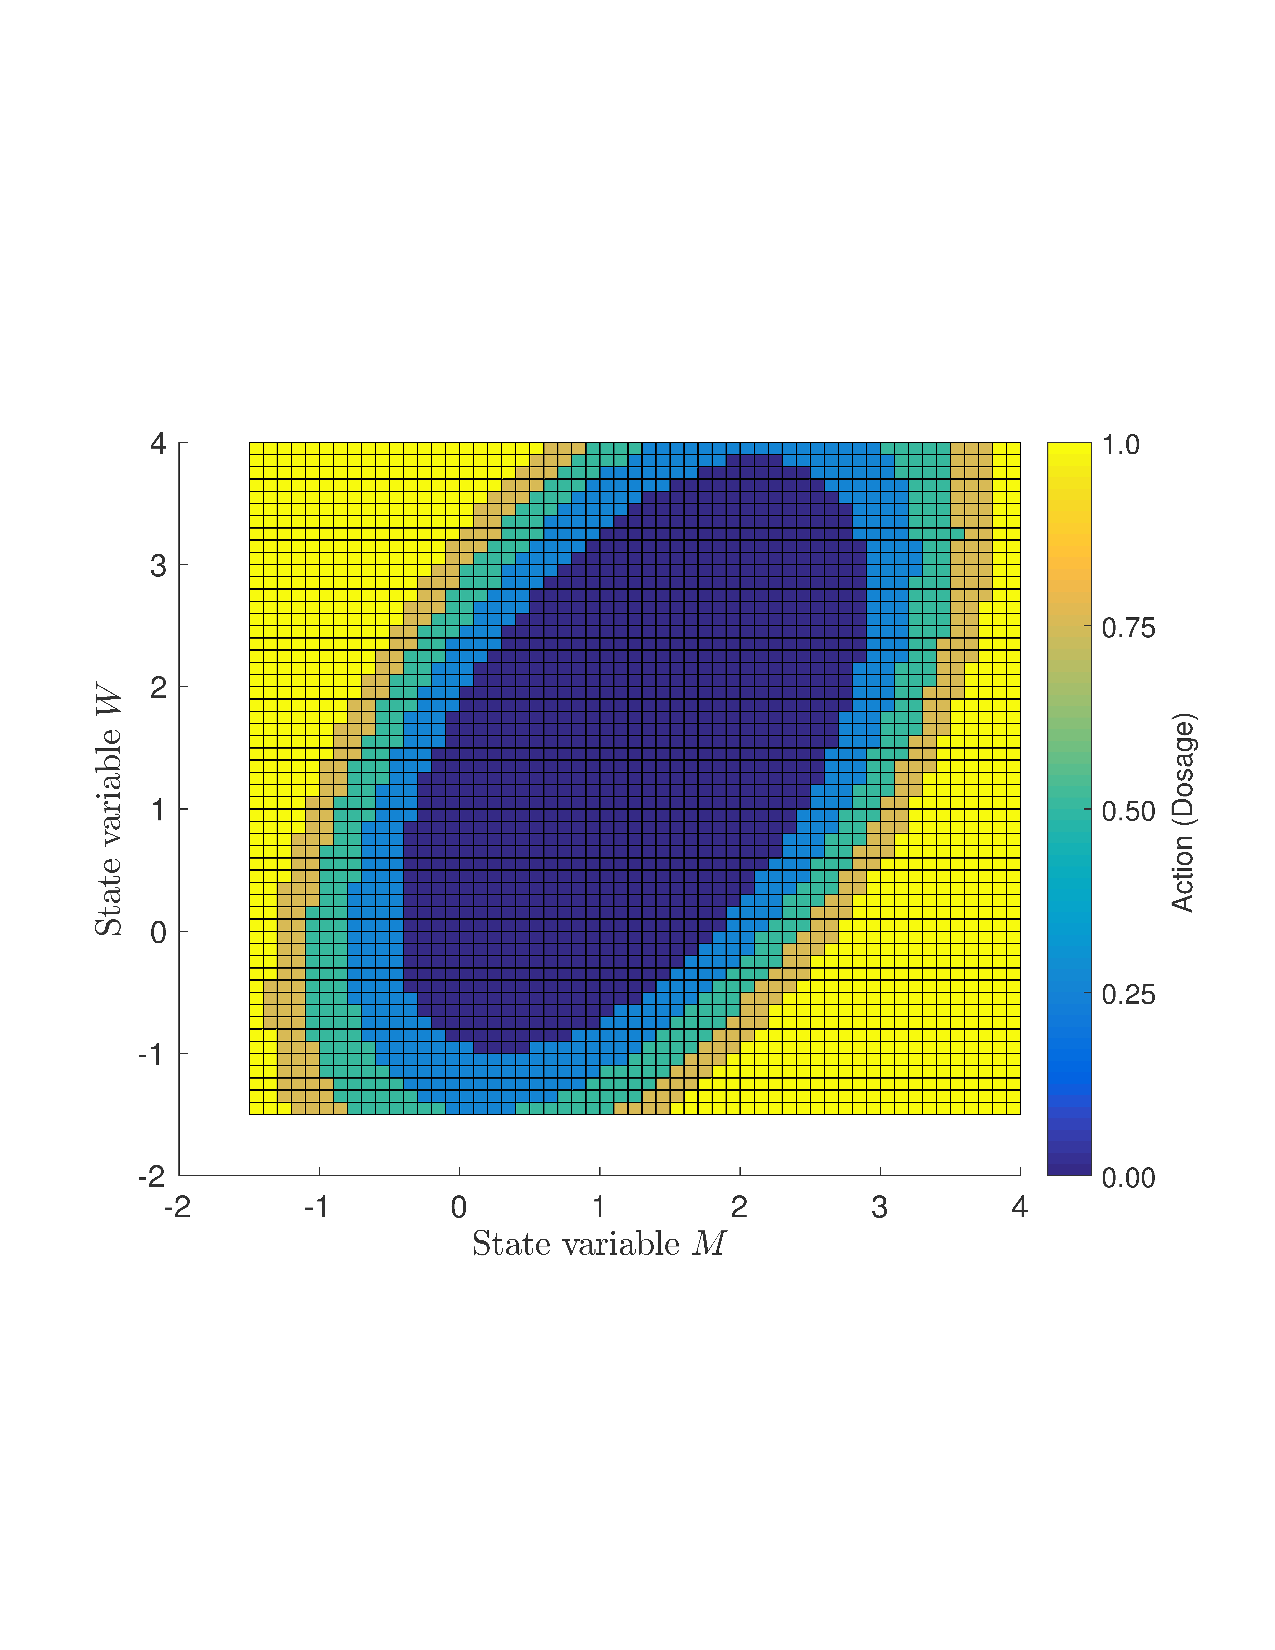
\includegraphics[width=.9\linewidth]{./Chapter-4/figs/action_nu5.pdf}
%	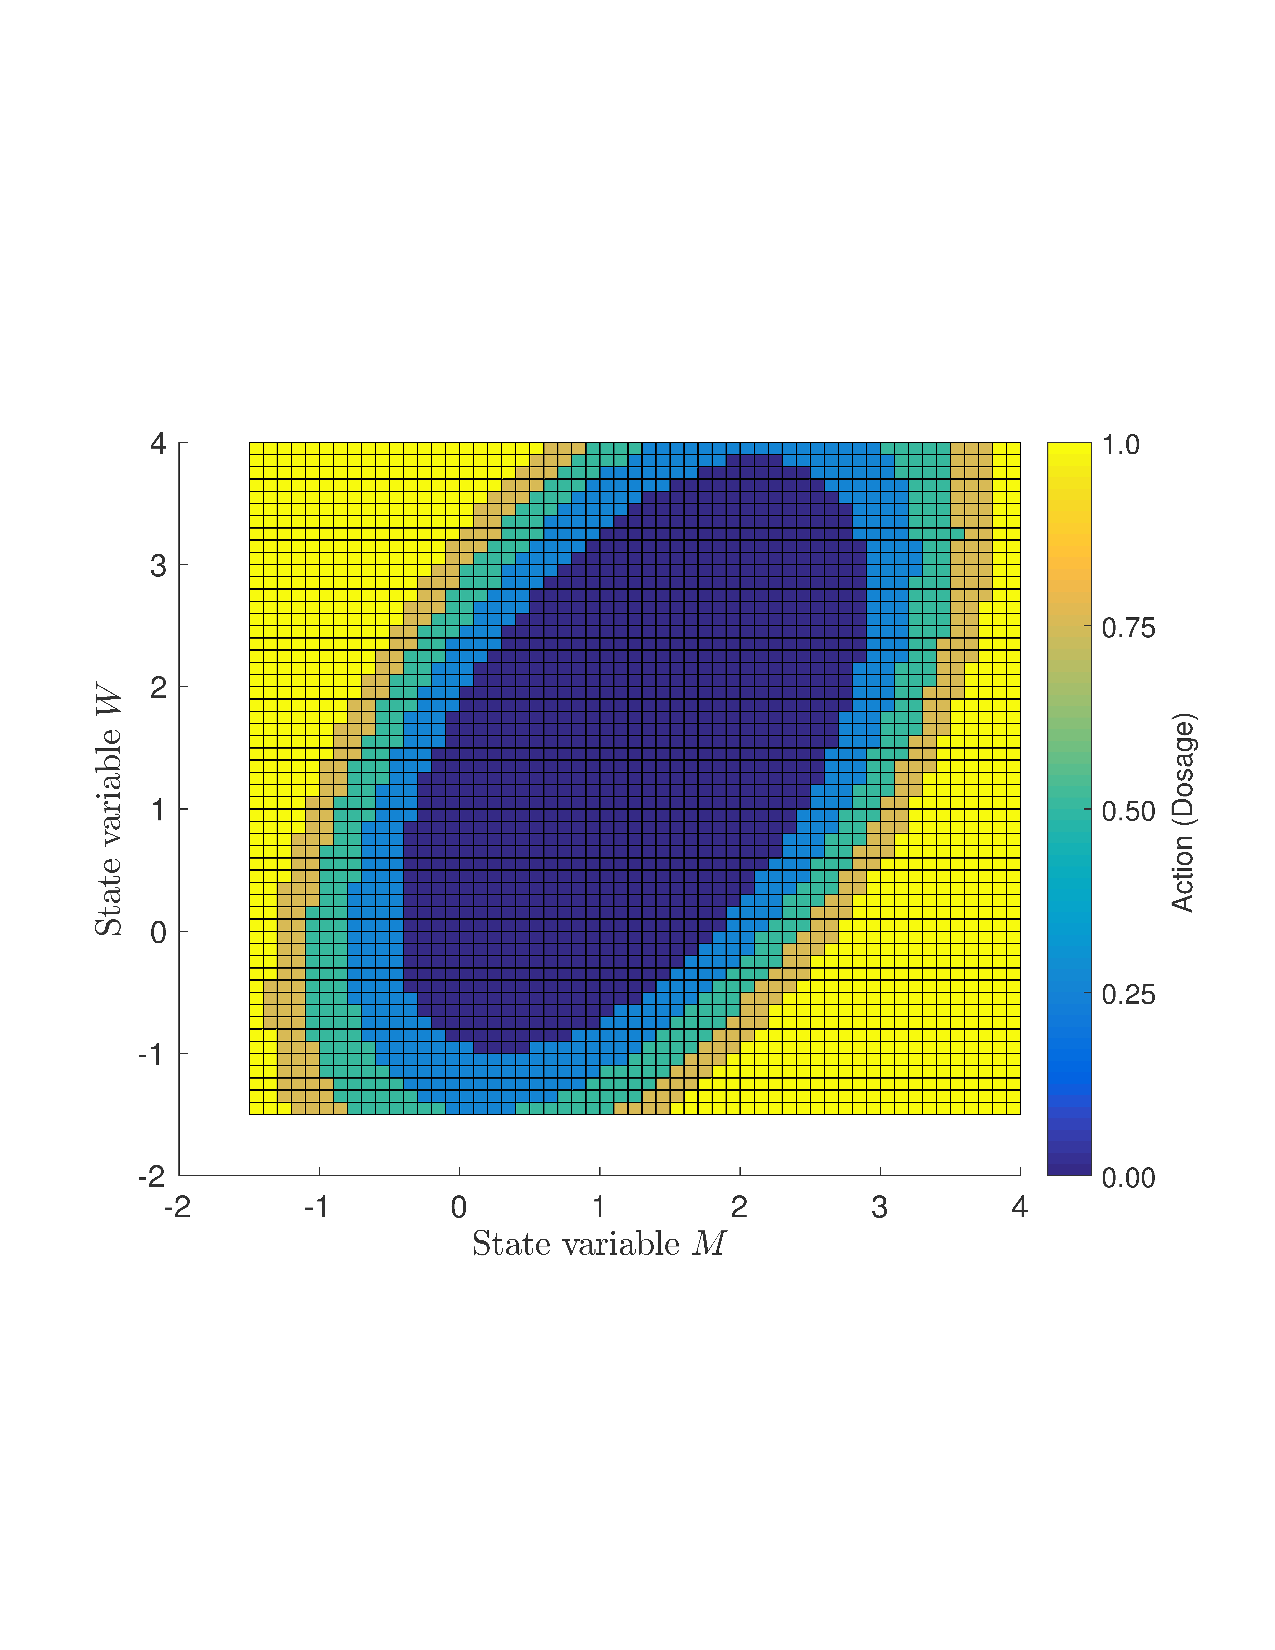
\includegraphics[width=.9\linewidth]{./Chapter-4/figs/action_nu5.pdf}
%	\caption{Action for each state under constraint bounds $\nu$}
%	\caption*{The red dotted line is for the primary outcome to maximized. The blue dotted line is for the secondary outcome to be constrained.}
%	\label{fig:1}
%\end{figure}
%\begin{minipage}{\linewidth}
%	\centering
	\begin{minipage}{0.95\linewidth}
		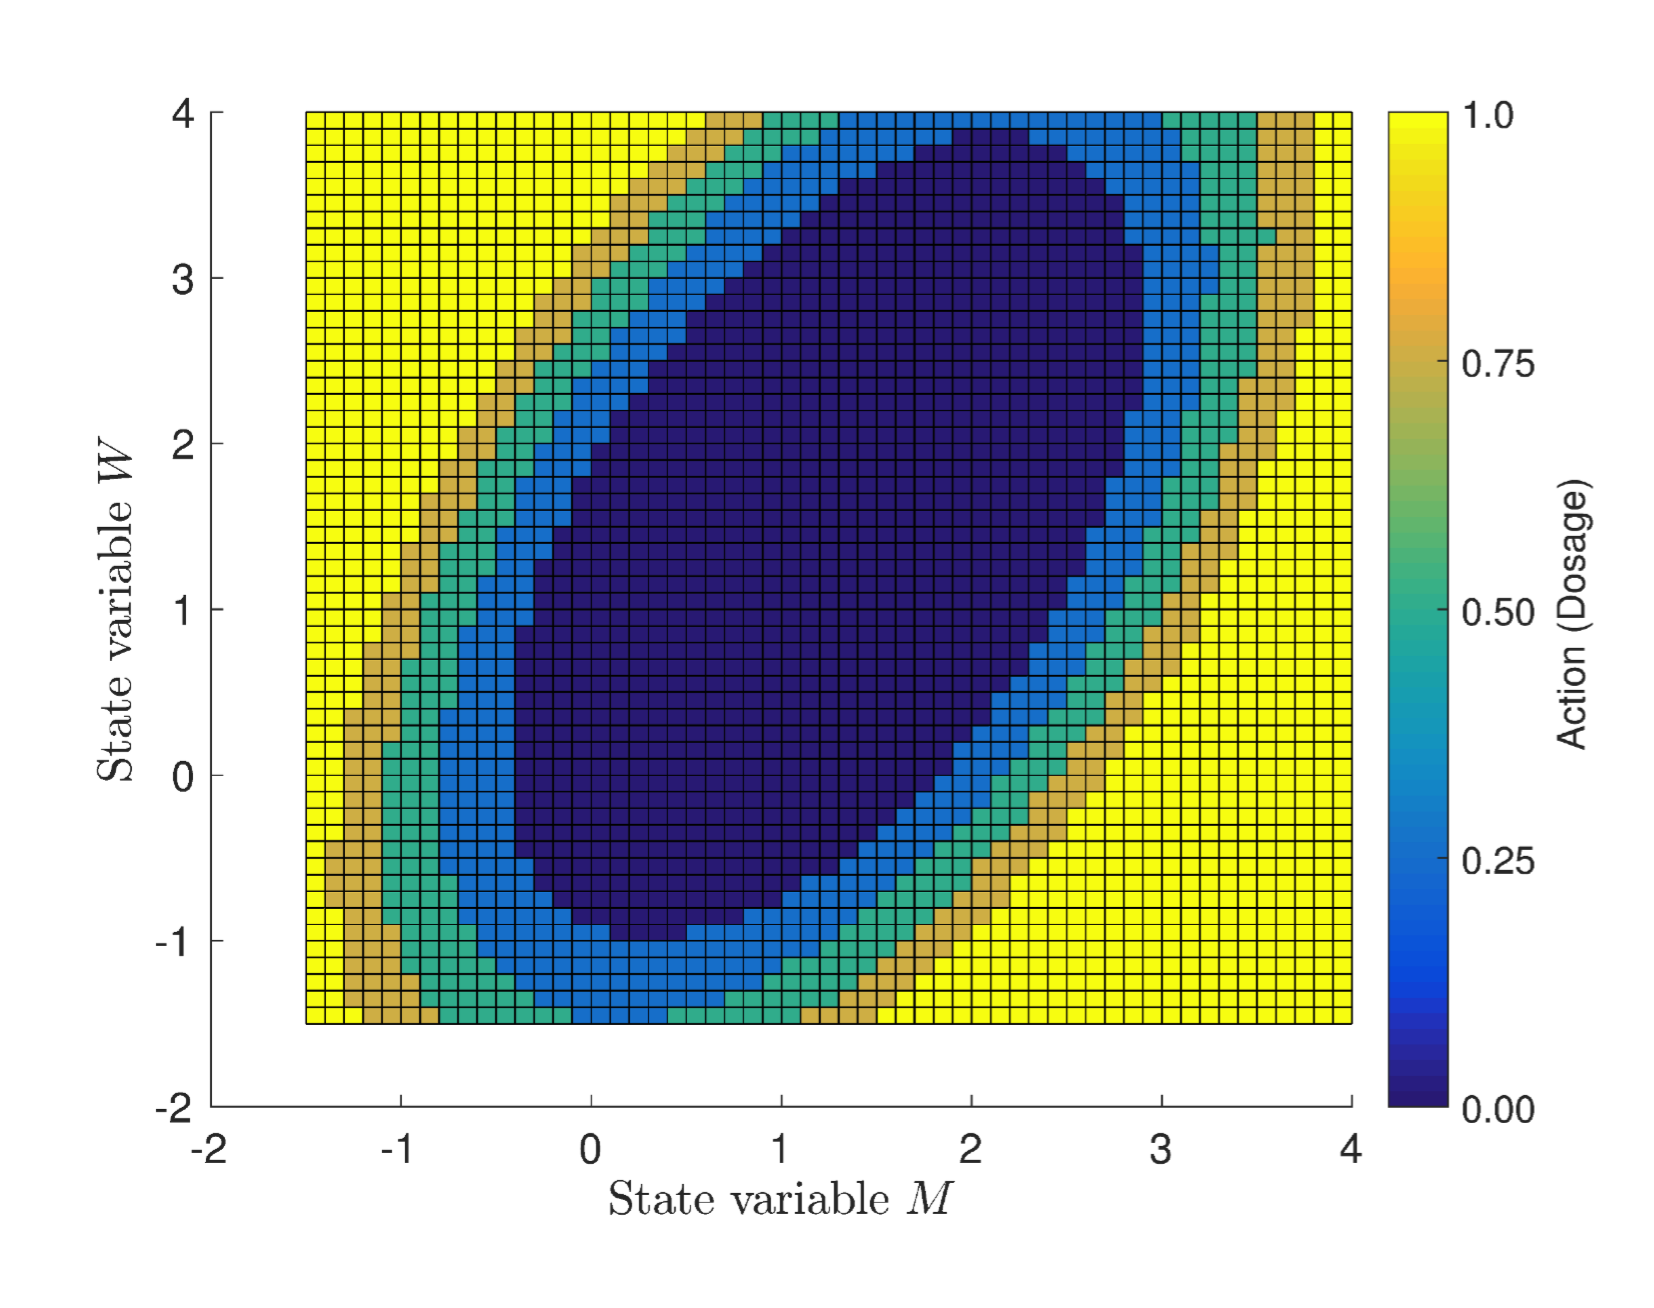
\includegraphics[width=\linewidth]{./Chapter-3/figs/action_nu5.png}
		\captionof{figure}{ Action for each state under constraint $\nu=10.93$}
		\caption*{Yellow represents high dosage treatment assignment. Blue represents low dosage assignment. As the constraint bound gets loose, more higher dosage treatments are assigned to patients.}
	\end{minipage}
	\newpage
	\begin{minipage}{0.95\linewidth}
		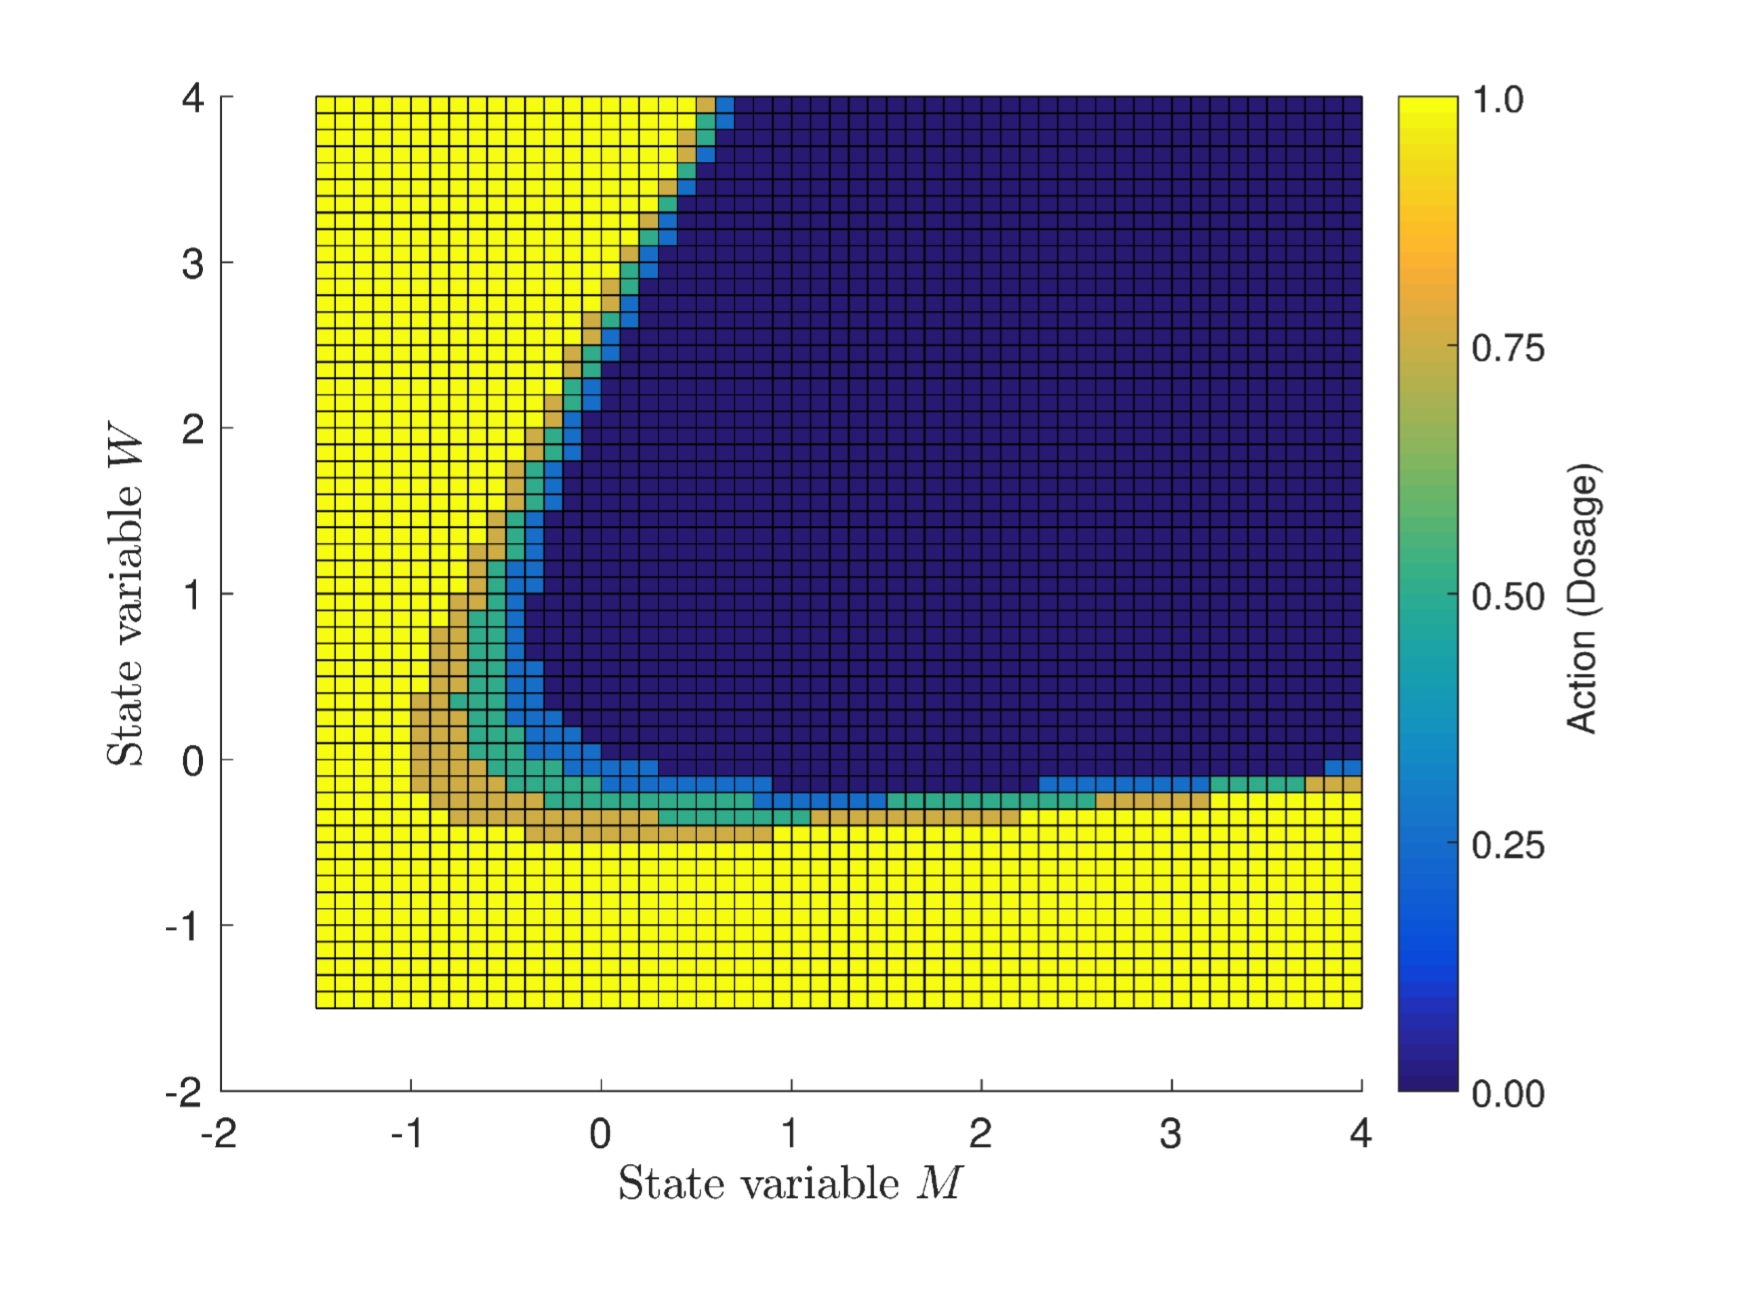
\includegraphics[width=\linewidth]{./Chapter-3/figs/action_nu10.png}
		\captionof{figure}{Action for each state under constraint $\nu=17.73$}
		\caption*{Yellow represents high dosage treatment assignment. Blue represents low dosage assignment. As the constraint bound gets loose, more higher dosage treatments are assigned to patients.}
	\end{minipage}
		\newpage
	\begin{minipage}{0.95\linewidth}
		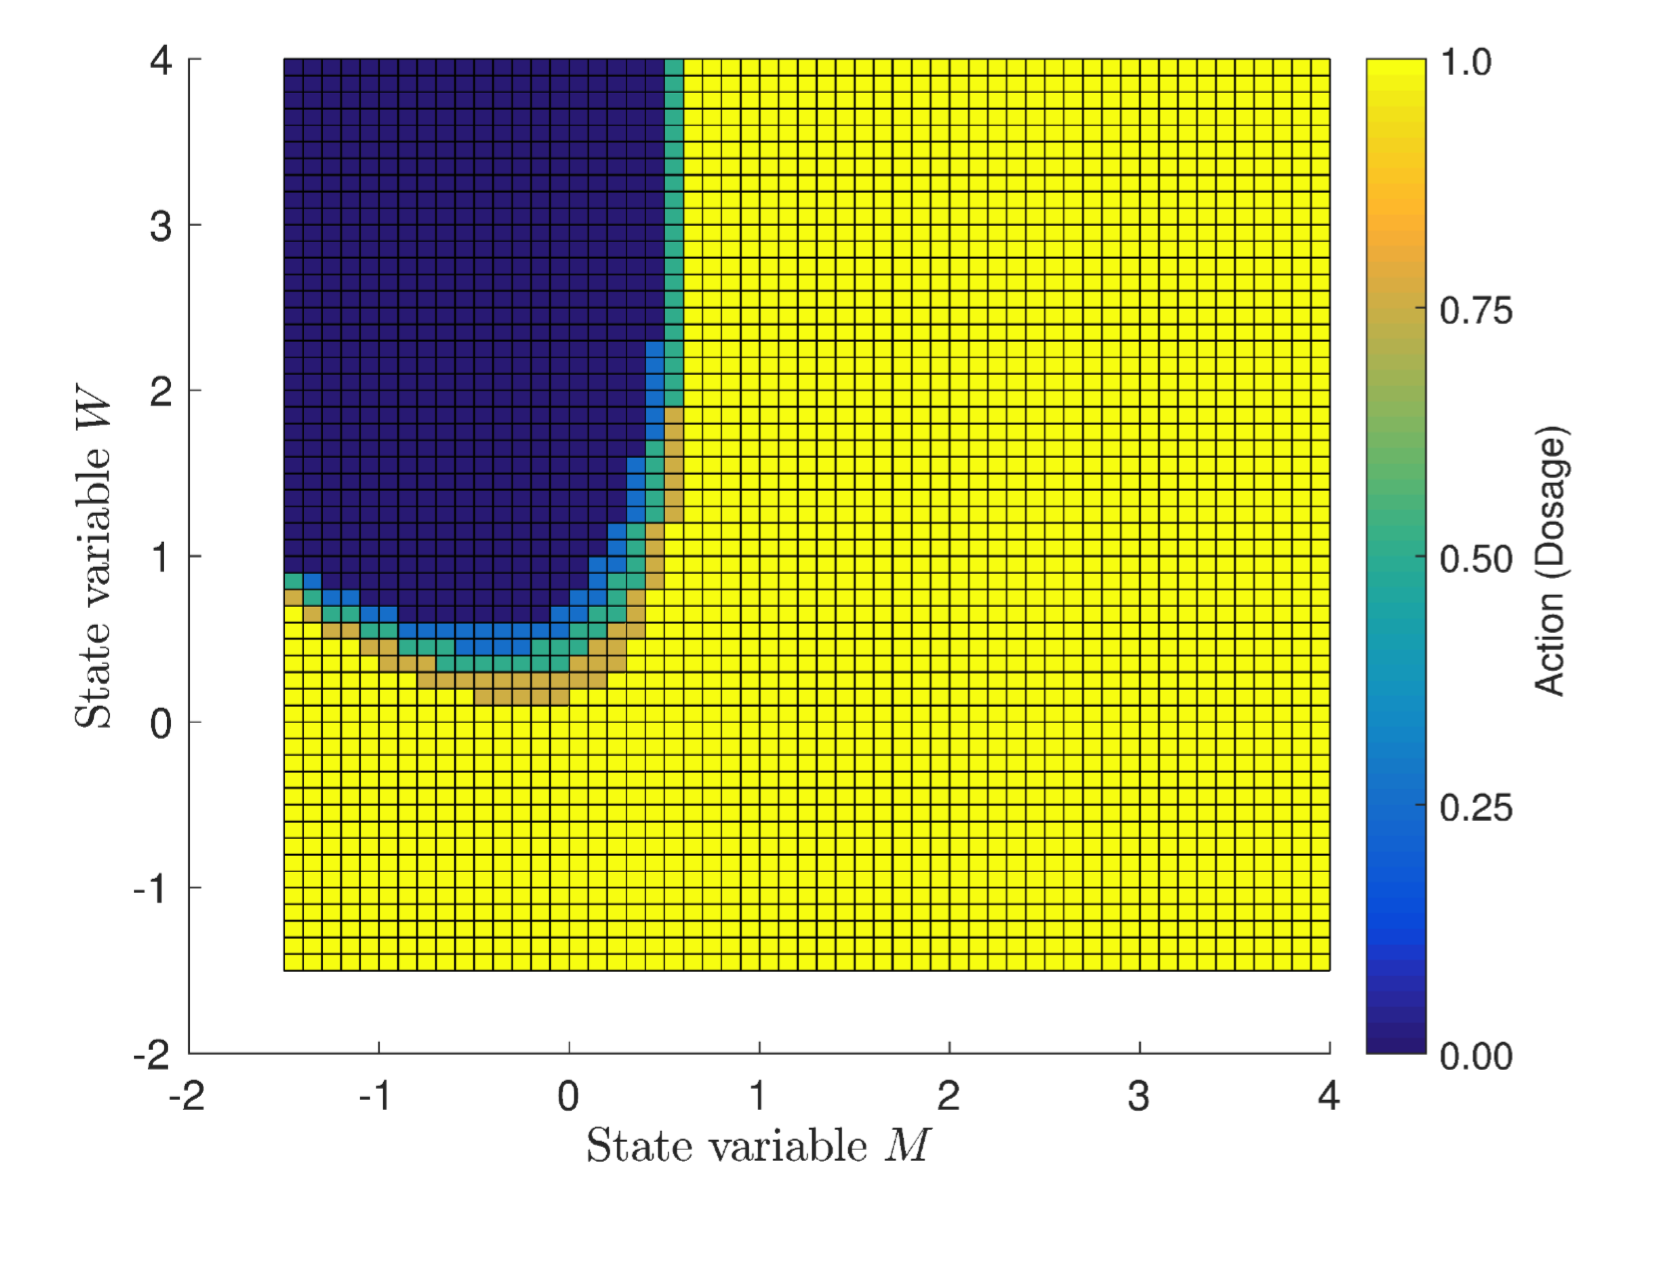
\includegraphics[width=\linewidth]{./Chapter-3/figs/action_nu15.png}
		\captionof{figure}{Action for each state under constraint $\nu= 24.54$}
		\caption*{Yellow represents high dosage treatment assignment. Blue represents low dosage assignment. As the constraint bound gets loose, more higher dosage treatments are assigned to patients.}
	\end{minipage}
		\newpage
	\begin{minipage}{0.95\linewidth}
		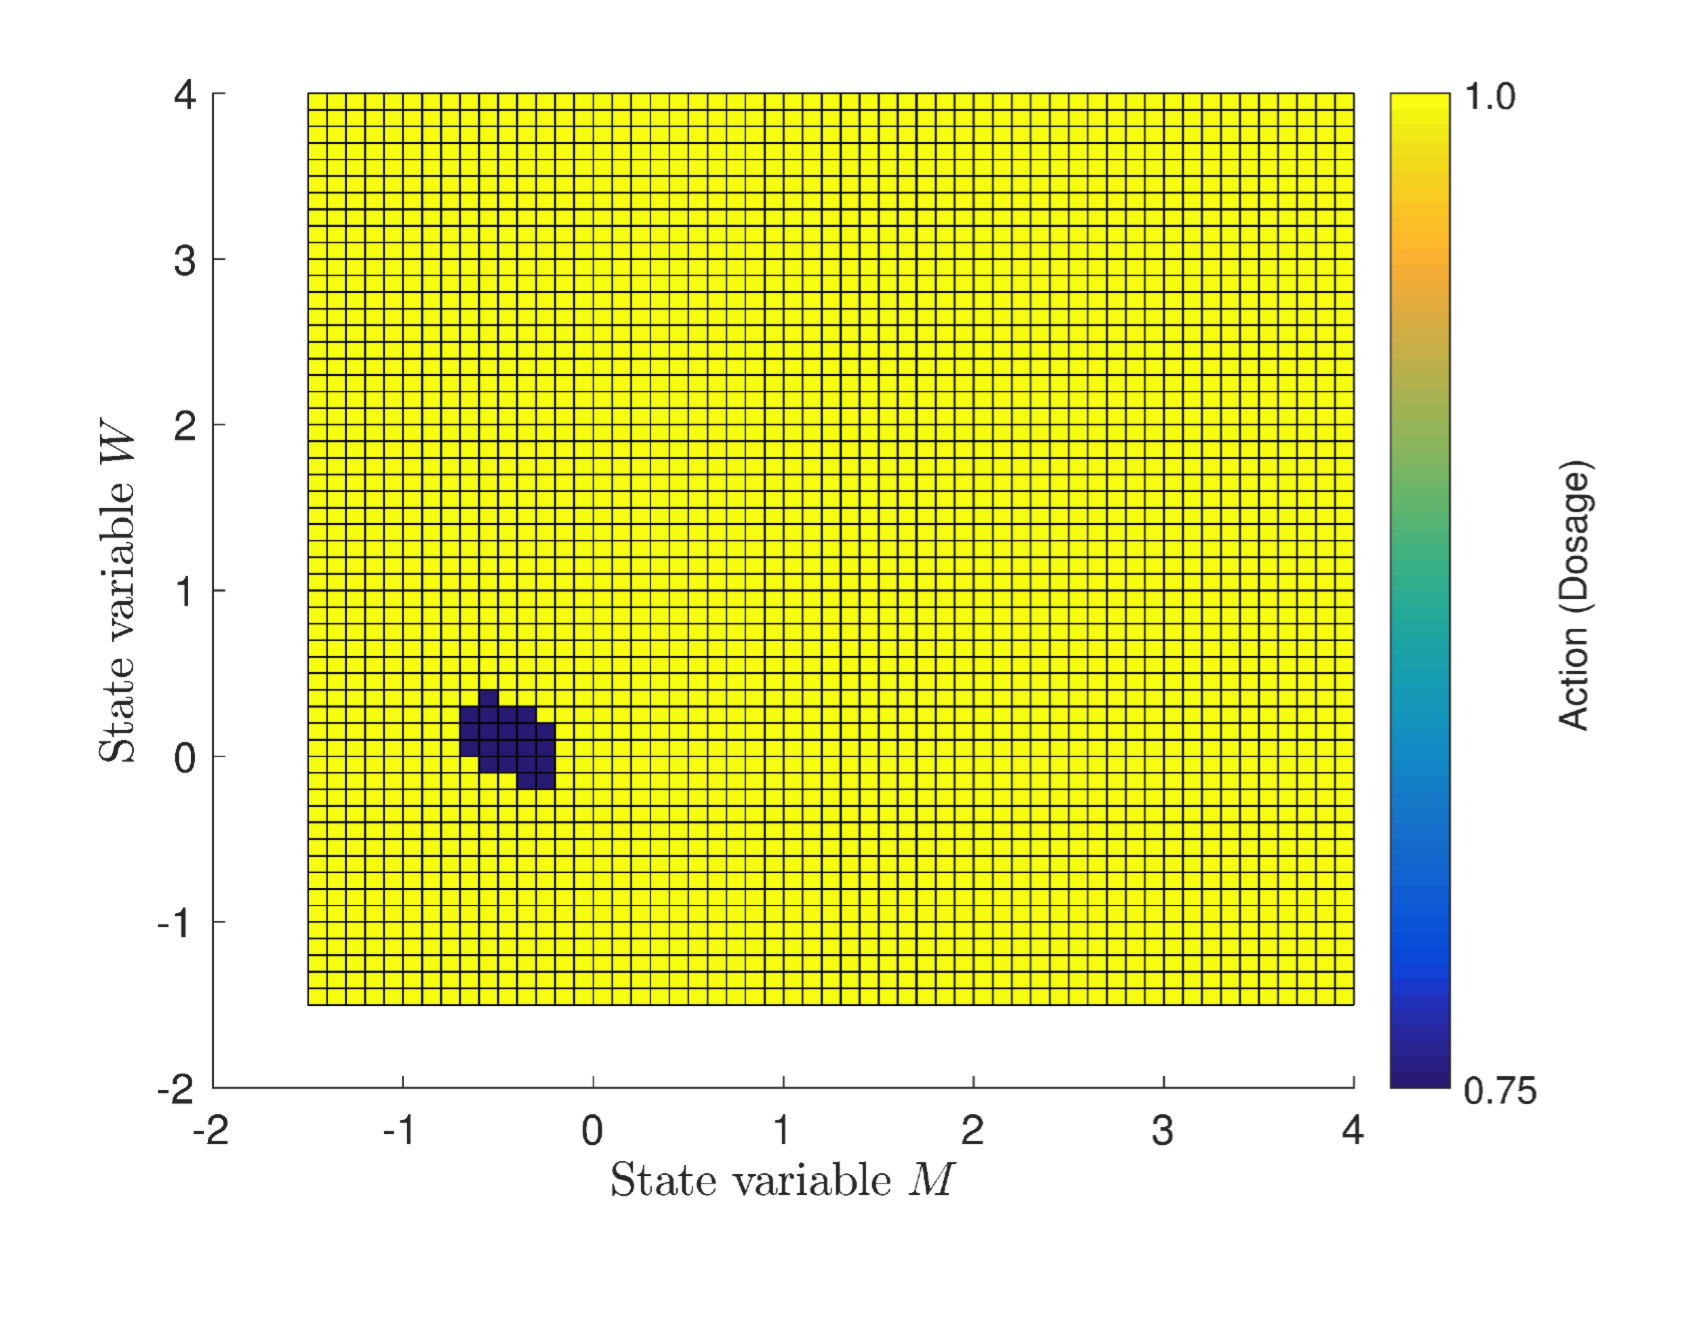
\includegraphics[width=\linewidth]{./Chapter-3/figs/action_nu20.png}
		\captionof{figure}{Action for each state under constraint $\nu=31.34$}
		\caption*{Yellow represents high dosage treatment assignment. Blue represents low dosage assignment. As the constraint bound gets loose, more higher dosage treatments are assigned to patients.}
	\end{minipage}
%\end{minipage}
\section{Conclusion and Future}
We propose a framework for constrained optimal dynamic treatment regimes to handle the trade-off between the primary objective and all other secondary objectives in infinite stage setting. The simulation results based on the chemotherapy ODE system are presented and visualized. This framework offers an intuitive way for clinicians to exam the trade-off and make treatment decisions based on patient's preference. Different from CPO, our method takes into consideration that clinical data is expensive and scarce. Borrowing strength from least-squares policy evaluation, our method is able to learn from data efficiently. Moreover, least-squares policy evaluation is an iterative method for policy evaluation, and has the advantage of being able to learn both offline and online. Hence, our method can fits in not only the situation where clinical policies needed to be learned after data collect (offline, off-policy batched), but also the situation where online real-time policy learning is needed. Interior-point method is also a well-studies optimization method for constrained estimation. Its theoretical guarantees assure us of good enough optimal solutions. However, it is obvious that the choice of policy function approximation may have impact on the decision. So does the choice of Q function approximation. Clinical domain expertise may required. Alternatively, automated feature learning techniques for function approximation from the machine learning community can be incorporated. More complex dataset maybe collected, such as text, image, speech and so on, considering the recent technology advancement in mobile devices. How to incorporate those complex information to better describe an individual's state of health is challenging. Rigorous theoretical work for our method is also under investigation.\\

Besides constraints on the expected value of a policy, we can also consider risk constraints, where the probabilities of adverse events occurring are restricted. Although reinforcement learning is a powerful technique to find optimal treatment regimes for clinical practice, designing appropriate reward functions is crucial for serving the desired clinical purpose, but very difficult. Current approach may not scale well in complex clinical situations or preventive healthcare where multiple subgoals may be involved. How to automatic generate rewards and objectives in complex clinical situations can be an interesting direction for investigation.\\

Nowadays, many aspects of the clinical practice have been transformed by mobile devices, such as smart phones, tablets, wearable sensors etc. It allows clinicians remotely monitor and intervene patients’ chronic conditions in real-time. It also allows for adaptive preventive interventions for motivating and maintaining healthy behaviors, such as physical exercise, diets, and so on. To better understand adaptive interventions, interdisciplinary collaborations becomes a necessity among clinicians, medical researchers, behavioral scientists, statisticians, and computer scientists.\\

% Preventive healthcare can be a possible application. thods to avoid occurrence of disease either through eliminating disease agents or increasing resistance to disease.[15] Examples include immunization against disease, maintaining a healthy diet and exercise regimen, and avoiding smoking.[16]
 % Rewards signal can be sparse as well. agent to automatically discover the range of tasks that it is capable of performing. We use a generator network to propose tasks for the agent to try to achieve, specified as goal states. The generator network is optimized using adversarial training to produce tasks that are always at the appropriate level of difficulty for the agent. Our method thus automatically produces a curriculum of tasks for the agent to learn. We show that, by using this framework, an agent can efficiently and automatically learn to perform a wide set of tasks without requiring any prior knowledge of its environment. Our method can also learn to achieve tasks with sparse rewards, which traditionally pose significant challenges.

% Automatic Goal Generation for Reinforcement Learning Agents. David Held, Xinyang Geng, Carlos Florensa, Pieter Abbeel

% In this paper, we consider Markov Decision Processes (MDPs) with error states. Error states are those states entering which is undesirable or dangerous. We define the risk with respect to a policy as the probability of entering such a state when the policy is pursued  \\




%%---------------------------------------------------------------------------%%
%%  Bibliography 

%%  You can use the bibitem list.
%\bibliographystyle{unsrt}
%\begin{thebibliography}{99}
%\bibitem{cb02}
%Casella, G. and Berger, R.L. (2002)
%\newblock {\it Statistical Inference, Second Edition.}
%Duxbury Press, Belmont, CA.
%
%\bibitem{t06}
%Tsiatis, A.A. (2006)
%\newblock {\it Semiparametric Theory and Missing Data.}
%Springer, New York.
%
%\end{thebibliography}

%% or use BibTeX
\bibliography{ShupingR-thesis}{}
\bibliographystyle{plain}

%%---------------------------------------------------------------------------%%
% Appendices
\appendix

\chapter{Supplement materials for Chapter 1}
\section{Conditions for convergence of the penalty-barrier trajectory for mixed constraints}
We revisit the conditions under which the  penalty-barrier trajectory converging to the solution to the original mixed-constraint problem. The original inequality-equality constrained problem is 
\begin{align}
\begin{split}
&\underset{\bs{x} \in \mb{R}^n}{\text{minimize }}f\lt(\bs{x}\rt)\\
\text{subject to }&  c_i\lt(\bs{x}\rt) \ge 0, i\in \mathcal{I} \text{, and } c_j\lt(\bs{x}\rt) = 0, j \in \mathcal{E} ,
\end{split}
\end{align}
where $\mathcal{I}$ is the set of the indices for inequality constraints, and $\mathcal{E}$ is the set of the indices for equality constraints. Let $\bs{x}^*$ denote a solution to the original problem (A.1). A classical strategy to solve this mixed constraint problem is to find an unconstrained minimizer of a composite function that consists of the objective function, the barrier penalty for the inequality constraints, and the quadratic penalty for the equality constraints, i.e., a penalty-barrier function. It is defined as
\begin{align}
\Phi_{PB}\lt(\bs{x}, \mu \rt) \triangleq f\lt(\bs{x}\rt) - \mu \underset{ i \in \mathcal{I}}{\sum} \text{log }c_i\lt(\bs{x}\rt) + \frac{1}{2\mu} \underset{j \in \mathcal{E}}{\sum}c^2_j\lt(\bs{x}\rt),
\end{align}
where $\mu$ is a sequence of sufficiently small, positive decreasing constants. Let $\bs{x}(\mu)$ denote an unconstrained minimizer of $\Phi_{PB}(\bs{x}, \mu)$. The following theorem gives the conditions that ensure the convergence of the differentiable penalty-barrier trajectory sequence $\lt\{ \bs{x}(\mu)\rt\}$ to the original solution $\bs{x}^*$.
\begin{theorem}[Second-Order Sufficient Conditions for Problem (A.1)~\cite{fiacco, Forsgren2002}]
	Sufficient conditions that a point $\bs{x}^*$ be an isolated (uniquely) local minimum of Problem (A.1), where $f$, $c_i, \, \forall i \in \mathcal{I}$, and $c_j, \forall j \in \mathcal{E}$ are twice-differentiable functions, are that there exist vectors $\lambda_{\mathcal{I}}^*$ and $\lambda_{\mathcal{E}}^*$ such that $\lt(\bs{x}^*, \lambda_{\mathcal{I}}^*, \lambda_{\mathcal{E}}^*\rt)$ satisfies
	\begin{enumerate}
		\item $\bs{x}^*$ is feasible and the LICQ (Linear Independence Constraint Qualification) holds at $\bs{x}^*$, i.e., the Jacobian matrix of active constraints at $\bs{x}^*$, $J_{\mathcal{A}}(\bs{x}^*)$, has full row rank;
		\item $\bs{x}^*$ is a KKT point and strict complementarity holds, i.e, the (necessarily unique) multiplier $\lambda^*$ has the property that $\lambda_i^* > 0$, for all $i  \in \mathcal{A}_{\mathcal{I}}(\bs{x}^*)$, the set of indices of active inequality constraints at $\bs{x}^*$;
		\item for all nonzero vectors $p$ satisfying $J_{\mathcal{A}}(\bs{x}^*)\bs{p} = 0$, there exists $\omega > 0$ such that $\bs{p}^{\itl}H(\bs{x}^*, \lambda^*) \bs{p} \ge \omega \|\bs{p}\|^2$., where $H(\bs{x}^*, \lambda^*) $ is the hessian of the Lagrangian at $\bs{x}^*$ and $\lambda^*$.
	\end{enumerate}
\end{theorem}
\begin{theorem}[Isolated Trajectory for $\Phi_{PB}(\bs{x}, \mu)$ Function~\cite{fiacco, Forsgren2002}]
	If (a) the functions $f$, $c_i, \forall i \in \mathcal{I}$, and $c_j, \,\forall j \in \mathcal{E}$ are twice differentiable, (b) the gradients $\nabla c_i, \,\forall i \in \mathcal{I}$, and $\nabla c_j, \forall j \in \mathcal{E}$ are linearly independent, (c) strict complementarity holds for  $u_i^* c_i (\bs{x}^*) = 0, \forall i \in \mathcal{I}$, and (d) the sufficient conditions stated above under which $\bs{x}^*$ be an isolated local constrained minimum of Problem (A.1) are satisfied by $\lt(\bs{x}^*, \lambda_{\mathcal{I}}^*, \lambda_{\mathcal{E}}^*\rt)$, then there is a positive neighborhood about $\mu = 0$ for which a unique-isolated differentiable function $\bs{x}(\mu)$ exists that describes a unique isolated trajectory of local minima of $\Phi_{PB}\lt(\bs{x}, \mu\rt)$, where $\bs{x}\lt(\mu\rt) \to \bs{x}^*$ as $\mu \to 0$.
\end{theorem}
Note that $c_i\lt(\bs{x}\rt), \forall i \in \mathcal{I}$ is embedded  in the log operator, $c_i(\bs{x}_\mu)> 0$ is enforced implicitly.
\section{Proof of Theorem 1.1.2}
\begin{theorem}
	For any fixed $\mu$, assume 
	\begin{enumerate}
		\item Point-wise convergence of $\wh{v}_j(\bs{\theta})$ in probability:\\ For every $ \bs{\theta} \in \ml{F}(\bs{\Theta})$, we have $ \underset{n \to \infty}{\lim} \text{Pr} \lt\{ \mid v_j(\bs{\theta}) - \wh{v}_j(\bs{\theta}) \mid \le \epsilon_j \rt\}  = 1$, $\forall \epsilon_j > 0$, where $j = 1, \cdots, J$;
		\item Existence of a strict local minimizers of $\phi^{PB}_{\mu}\lt(\bs{\theta}\rt)$:\\
		There exists a neighborhood of $\bs{\theta}^{*}_{\bs{\nu}}(\mu)$, denoted $\ml{N}\lt(\bs{\theta}^{*}_{\bs{\nu}}(\mu)\rt)$ such that $\phi^{PB}_{\mu}\lt(\bs{\theta}^{*}_{\bs{\nu}}(\mu)\rt) < \phi^{PB}_{\mu}\lt(\bs{\theta}\rt)$, for any $\bs{\theta} \in \ml{N}\lt(\bs{\theta}^{*}_{\bs{\nu}}(\mu)\rt)$;
		\item Existence of strict local minimizer $\wh{\bs{\theta}}_{\bs{\nu}}(\mu)$ of $\wh{\phi}^{PB}_{\mu}\lt(\bs{\theta}\rt)$ in the neighborhood $\ml{N}\lt(\bs{\theta}^{*}_{\bs{\nu}}(\mu)\rt)$:\\  
		$ \wh{\phi}^{PB}_{\mu}\lt(\wh{\bs{\theta}}_{\bs{\nu}}(\mu)\rt) < \wh{\phi}^{PB}_{\mu}\lt(\bs{\theta}\rt)$, for any $\bs{\theta} \in \ml{N}\lt(\bs{\theta}^{*}_{\bs{\nu}}(\mu)\rt)$, where $\wh{\bs{\theta}}_{\bs{\nu}}(\mu) \in \ml{N}\lt(\bs{\theta}^{*}_{\bs{\nu}}(\mu)\rt)$;
	\end{enumerate} then 
	$$\wh{\bs{\theta}}_{\bs{\nu}}(\mu) \overset{p}{\to} \bs{\theta}^{*}_{\bs{\nu}}(\mu).$$
	%\begin{equation*}
	%\begin{aligned}
	%\underset{\bs{\theta} \in \ml{F}(\bs{\Theta})}{\sup} \mid \wh{\phi}^{PB}_{\mu}(\bs{\theta}) - \phi^{PB}_{\mu}(\bs{\theta})\mid = o_{p}(1).
	%\end{aligned}
	%\end{equation*}
	
	%Assume 1 - 3 in Lemma 1.1.2 hold, and then, for any fixed $\mu$,
	%\begin{equation*}
	%\begin{aligned}
	%\wh{\bs{\theta}}_{\bs{\nu}}(\mu) \overset{p}{\to} \bs{\theta}^{*}_{\bs{\nu}}(\mu).
	%\end{aligned}
	%\end{equation*}
\end{theorem}

\begin{proof}
	In this part, we simplify the notations locally just for this proof. Suppose there exists a local minimum $\bs{\theta}^{*} = \bs{\theta}^{*}_{\bs{\nu}}(\mu)$. Let its estimator be $ \wh{\bs{\theta}} = \wh{\bs{\theta}}_{\bs{\nu}}(\mu)$ and its neighborhood $\ml{N}^{*} = \ml{N}\lt(\bs{\theta}^{*}_{\bs{\nu}}(\mu)\rt)$. Also, let $\phi\lt(\bs{\theta}\rt) = \phi^{PB}_{\mu}\lt(\bs{\theta}\rt)$ and $\wh{\phi}(\bs{\theta}) = \wh{\phi}^{PB}_{\mu}\lt(\bs{\theta}\rt)$.
	By assumption 1, $\lvert \phi(\bs{\theta}^*) - \wh{\phi}(\bs{\theta}^*) \rvert = o_p(1)$, as $n \to \infty$; $\lvert \phi(\wh{\bs{\theta}}) - \wh{\phi}(\wh{\bs{\theta}}) \rvert = o_p(1)$, as $n \to \infty$. Both $\bs{\theta}^* \in \ml{N}^*$ and $\wh{\bs{\theta}} \in \ml{N}^*$ .
	\begin{flalign*} 
	\phi(\bs{\theta}^*) & = \wh{\phi}(\widehat{\bs{\theta}}) + \lt\{\phi(\bs{\theta}^*) - \wh{\phi}(\widehat{\bs{\theta}})\rt\} \\
	& > \wh{\phi}(\widehat{\bs{\theta}}) + \lt\{\phi(\bs{\theta}^*) - \wh{\phi}(\bs{\theta}^*)\rt\} \text{ (by assumption 3) }\\
	& \ge \wh{\phi}(\widehat{\bs{\theta}}) - \lvert \phi(\bs{\theta}^*) - \wh{\phi}(\bs{\theta}^*)\rvert \\
	& = \phi(\widehat{\bs{\theta}}) + \lt\{\wh{\phi}(\widehat{\bs{\theta}}) - \phi(\widehat{\bs{\theta}})\rt\}  - \lvert \phi(\bs{\theta}^*) - \wh{\phi}(\bs{\theta}^*)\rvert \\
	& \ge \phi(\widehat{\bs{\theta}}) - \lv \wh{\phi}(\widehat{\bs{\theta}}) - \phi(\widehat{\bs{\theta}})\rv - \lvert \phi(\bs{\theta}^*) - \wh{\phi}(\bs{\theta}^*)\rvert \\
	& \ge \phi(\widehat{\bs{\theta}}) + o_p(1) \text{ (implied by assumption 1) }
	\end{flalign*}
	Suppose $\wh{\bs{\theta}} \not\to \bs{\theta}^*$, and then $\phi(\bs{\theta}^*) > \liminf \phi(\wh{\bs{\theta}})$. This is opposed to assumption 2, which claims $\bs{\theta}^*$ to be a strict local minimizer. By contradictory, it is proven that $\wh{\bs{\theta}} \overset{p}{\to} \bs{\theta}^*$, as $n \to \infty$.
\end{proof}
\section{Consistency of Kernel Density Estimators}
As kernel density estimators (KDEs) are used to estimate values of regimes, we review the necessary asymptotic properties of Kernel Density Estimators briefly here.
\subsection{Consistency of univariate Kernel Density Estimator }
We review uniform consistency of Kernel Density Estimators for a univariate distribution $g(x)$ ~\cite{Silverman1978a,Pagan1999}. Consider the kernel estimate $\widehat{g}_n(x)$ of a real univariate density $g(x)$ introduced by Rosenblatt (1956) ~\cite{Silverman1978a,Pagan1999},  and defined as 
$$\widehat{g}_n(x) = \sum_{i=1}^{n} \frac{1}{nh} k\left( \frac{x-X_i}{h}\right),$$
where $X_1, \cdots, X_n$ are identically independent observations from the  distribution $g(x)$; $k$ is a kernel function satisfying suitable conditions given below; $h = h_n$ is the bandwidth which is also a function of sample size $n$.
\begin{theorem}[Uniform consistency of univariate Kernel Density Estimators]~\cite{Pagan1999,Silverman1978a}
	If all the following assumptions hold,
	\begin{enumerate}
		\item If the kernel density function $k(s)$ satisfies
		\begin{enumerate}
			\item $\int k(s)\,ds=1$;
			\item $\int \mid k(s) \mid \,ds<\infty$;
			\item $\left|s\right|\left|k(s)\right| \to 0,$ as $s \to \infty$;
			\item $\sup\left|k(s)\right|<\infty$.
			%\item $\int k^{2}(s)\,ds<\infty$.
		\end{enumerate}
		\item The bandwidth $h$ satisfies that $h \to 0$ and $nh^2 \to \infty$, as $n \to \infty$;
		\item $g(x)$ is uniformly continuous on $\mathbb{R}$;
		\item The characteristic function $\phi(t)$ of a random variable $s$ with the density $k(s)$,  $\psi(t) = \int e^{its} k(s)\,ds$, is absolutely integrable,
	\end{enumerate}
	and then we have that $\widehat{g}_n(x)$ is uniformly weak consistent, that is, 
	$$\underset{n \to \infty}{p\lim} \left[\underset{x}{\sup} \mid \widehat{g}_n(x) - g(x) \mid  \right] = 0,$$
	where $\underset{n \to \infty}{p\lim}$ denotes convergence in probability.
\end{theorem} 
\subsection{Consistency of multivariate Kernel Density Estimator }
The uniform convergence theorem of univariate Kernel Density Estimators above is extended to multivariate case by Cacoullos (1964)~\cite{Theo}. Consider an estimator of a $d$-dimensional density function $g(\boldsymbol{x})$ of the following form:
\begin{gather*}
\widehat{g}_n(\boldsymbol{x}) = \frac{1}{h^{d}} \sum_{i=1}^{n}\bar{k}\left( \frac{\boldsymbol{x} - \boldsymbol{X}_i}{h}\right)
\end{gather*}
where $\bar{k}(\boldsymbol{s})$ is a multivariate kernel of choice satisfying suitable conditions given below, and $h = h_n$ is the bandwidth. 
\begin{theorem}[Uniform consistency of multivariate Kernel Density Estimators]~\cite{Theo}
	Assume:
	\begin{enumerate}
		\item $\bar{k}(\boldsymbol{s})$ is a Borel scalar function on $\mathbb{R}^{d}$, where $\boldsymbol{s} := (s_1, \cdots, s_{d})$ such that 
		\begin{enumerate}
			\item $\idotsint \bar{k}(\boldsymbol{s}) \,ds_1\cdots \,ds_{d} = 1$;
			\item $\idotsint | \bar{k}(\boldsymbol{s}) | \,ds_1\cdots \,ds_{d}<\infty$;
			\item $|\boldsymbol{s}|^{d}|\bar{k}(\boldsymbol{s})| \to 0,$ as $\boldsymbol{s} \to \infty$, where $|\boldsymbol{s}|$ is the length of $\boldsymbol{s}$;
			\item $\underset{\boldsymbol{s}}{\sup} | \bar{k}(\boldsymbol{s}) | < \infty$.
		\end{enumerate}
		\item $h \to 0$ and $nh^{2d} \to \infty$, as $n \to \infty$;
		\item $g(\boldsymbol{x})$ is uniformly continuous in $\mathbb{R}^{d}$;
		\item The characteristic function of a random vector $\boldsymbol{s}$ with the density  of $\bar{k}(\boldsymbol{s})$, $\psi(\boldsymbol{t}) = \idotsint e^{i\boldsymbol{t}^{\intercal}\boldsymbol{s}} \bar{k}(\boldsymbol{s})\,d\boldsymbol{s}$,  is absolutely integrable,
	\end{enumerate}
	and then, $\widehat{g}_n(\boldsymbol{x})$ is uniform consistent, that is,
	\begin{gather*}
	\underset{n \to \infty}{p\lim}  \left[ \underset{\boldsymbol{x}}{\sup} \left|\widehat{g}_n(\boldsymbol{x}) - g(\boldsymbol{x}) \right| \right] = 0.
	\end{gather*}
\end{theorem}
Usually, we use a product kernel for multivariate distributions. For random vector $\boldsymbol{S}  \in \mathbb{R}^{d}$, $\boldsymbol{S} := ( S_1, \cdots, S_{d})$,
\begin{flalign*}
\frac{1}{h^{d}}\bar{k}\left(\frac{\boldsymbol{s}}{h}\right) = \frac{1}{h^{d}}\prod_{j=1}^{d}k\left(\frac{s_j}{h}\right),
\end{flalign*}
where $k(s)$ is a suitable univariate kernel function. Here, we exposit the bandwidths for each component with the same magnitude, $h_n = h$. which is also inferred by optimal bandwidth choice.
%\section{Estimating the value functions via KDE}
%We derive the value function estimator using KDE. Recall the $j$-th value function is modeled as $$V_j\lt(\bs{\theta}\rt) = m_{\bs{\alpha}^*_j}+ \iint \tsgn\lt(z_1\rt)z_2 f_{\bs{\beta}^*_j}\lt(z_1, z_2; \bs{\theta}\rt) \,dz_1 \,dz_2,$$ 
%Note, for any fixed $\bs{\beta}_j$, {\small$\iint\text{sgn}(z_1)z_2\,f_{\bs{\beta}_j}\left(z_1,z_2;\bs{\theta}\right)\,dz_1\,dz_2 =  2\iint z_2\,\mathbb{I}\left(z_1\ge0\right)\,f_{\bs{\beta}_j}\left(z_1, z_2;\bs{\theta}\right)\,dz_1\,dz_2-\int z_2\,f_{\bs{\beta}_{j}}\left(z_2\right)\,dz_2.$} To estimate this quantity, we plug in kernel density estimators for $f_{\bs{\beta}_j}(z_1, z_2; \bs{\theta})$
%and $f_{\bs{\beta}_j}( z_2 )$, and get
%
%\begin{equation}
%	\begin{aligned}
% & \iint \tsgn\lt(z_1\rt)z_2 \wh{f}_{\bs{\beta}_j}\lt(z_1, z_2; \bs{\theta}\rt) \,dz_1 \,dz_2\\
%=&2\iint z_2\,\mathbb{I}\left(z_1\ge0\right)\,\wh{f}_{\bs{\beta}_j}\left(z_1, z_2;\bs{\theta}\right)\,dz_1\,dz_2-\int z_2\,\wh{f}_{\bs{\beta}_{j}}\left(z_2\right)\,dz_2\\
%= &2\iint z_2\,\mathbb{I}\left(z_1\ge0\right)\lt\{\frac{1}{nh^2}\sum_{i=1}^{n}k\left(\frac{z_1-Z^i_1}{h}\bigg)k\bigg(\frac{z_2-Z^{i}_2}{h}\right)\rt\}\,dz_1\,dz_2-\int z_2\lt\{\frac{1}{nh}\sum_{i=1}^{n}k\left(\frac{z_2-Z^{i}_2}{h}\right)\rt\}\,dz_2\\
%=  &\frac{2}{n}\sum_{i=1}^{n}\bs{X}_{1}^{i\intercal}\bs{\beta}_{j}\left\{ 1-K\left(-\frac{\bs{X}^{i\intercal}\bs{\theta}}{h}\right)\right\} -\frac{1}{n}\sum_{i=1}^{n}\bs{X}_{1}^{i\intercal}\bs{\beta}_{j}\\
%= &\frac{1}{n}\sum_{i=1}^{n}\bs{X}_{1}^{i\intercal}\bs{\beta}_{j}\left\{ 1-2K\left(-\frac{\bs{X}^{i\intercal}\bs{\theta}}{h}\right)\right\},
%\end{aligned}
%\end{equation}
%where $K(s)$ is the corresponding CDF of the kernel function $k(s)$.The third equality is derived in the following. As we use the Gaussian kernel for $k(s)$, it satisfies the following
%\begin{enumerate}
%	\item $\int_{-\infty}^{\infty}k(s)\,ds=1$;
%	\item $k(s)>0$ for all $s$;
%	\item $k(-s)=k(s)$ for all $s$; 
%	\item The first order derivative of the kernel, $k^{\prime}(s)$, exists and is bounded. 
%\end{enumerate}
%To calculate the first term on the right hand side, let $s=\frac{z_1-Z_1^i}{h}$ and $t=\frac{z_2-Z^{i}_2}{h}$.
%Then, $z_1=Z^{i}_1+sh$ and $z_2=Z^{i}_2+th$. Also,
%$dz_1=h\,ds$ and $\,dz_2=h\,dt$. Then,
%\begin{flalign*} 
%&\frac{2}{h^2}\iint z_2\,\mathbb{I}\left(z_1\ge0\right)k\lt(\frac{z_1-Z^i_1}{h}\rt)k\lt(\frac{z_2-Z_2^{i}}{h}\rt)\,dz_1\,dz_2\\
%= & 2\iint\left(Z_2^i+th\right)\,\mathbb{I}\left(Z_1^i+sh\ge0\right)k\left(s\right)k\left(t\right)\,ds\,dt\\
%= & 2\iint Z_2^i\,\mathbb{I}\left(Z_1^i+sh\ge0\right)k\left(s\right)k\left(t\right)\,ds\,dt + 2\iint th \,\mathbb{I}\left(Z_1^i+sh\ge0\right)k\left(s\right)k\left(t\right)\,ds\,dt\\
%= &  2\int Z_2^i\,\mathbb{I}\left(s\ge -\sfrac{ Z_1^i}{h}\right)k\left(s\right)\,ds + 0 \\
%= &  2 Z_2^i \lt\{ 1 - K\lt(-\sfrac{Z_1^i}{h} \rt) \rt\} \\
%= & 2\bs{X}_{1}^{i\intercal}\bs{\beta}_{j}\left\{ 1-K\left(-\frac{\bs{X}^{i\intercal}\bs{\theta}}{h}\right)\right\},
%\end{flalign*}
%where $K\left(s\right)=\int k\left(s\right)\,ds+c$. The
%third equality holds, as $\int k(t)\,dt=1$ and $\int t\,k(t)\,dt=0$.
%The fourth equality holds as $\int\mathbb{I}\left(s\ge-\sfrac{Z_i}{h}\right)k\left(s\right)\,ds=1-\int_{-\infty}^{-\sfrac{Z^i_1}{h}}k\left(s\right)\,ds=1-K\left(-\sfrac{Z^i_1}{h}\right)$,
%where $Z^i_1=\bs{X}^{i\intercal}\bs{\theta}$ and  $Z^i_2=\bs{X}_1^{i\intercal}\bs{\beta}_j$.\\
%
%To calculate the second term on the right hand side, we derive $\frac{1}{h}\int z_2k(\frac{z_2-Z^i_2}{h})\,dz_2$ by changing variable similarly. Let $t=\frac{z_2-Z^i_2}{h}$
%,and we get $z_2=Z^i_2+th$ and $\,dz_2=h\,dt$. Then,
%\begin{flalign*}
%&\frac{1}{h}\int z_2k\left(\frac{z_2-Z^i_2}{h}\right)\,dz_2
%=  \int\left(Z^{i}_2+th\right)k\left(t\right)\,dt
%=  Z^{i}_2
%= \bs{X}_{1}^{i\intercal}\bs{\beta}_{j}.
%\end{flalign*}
%Again, the second equality holds as $\int k(t)\,dt=1$,
%and $\int t\,k(t)\,dt=0$. Together, we complete the derivation for (A.3).
%
\section{Estimating the value functions via KDE}
We derive the value function estimator using KDE. Recall the $j$-th value function is modeled as $$V_j\lt(\bs{\theta}\rt) = m_{\bs{\alpha}^*_j}+ \iint \tsgn\lt(z_1\rt)z_2 f_{\bs{\beta}^*_j}\lt(z_1, z_2; \bs{\theta}\rt) \,dz_1 \,dz_2,$$ 
Note, for any fixed $\bs{\beta}_j$, {\small$\iint\text{sgn}(z_1)z_2\,f_{\bs{\beta}_j}\left(z_1,z_2;\bs{\theta}\right)\,dz_1\,dz_2 =$\\$2\iint z_2\,\mathbb{I}\left(z_1\ge0\right)\,f_{\bs{\beta}_j}\left(z_1, z_2;\bs{\theta}\right)\,dz_1\,dz_2-\int z_2\,f_{\bs{\beta}_{j}}\left(z_2\right)\,dz_2.$} To estimate this quantity, we plug in kernel density estimators for $f_{\bs{\beta}_j}(z_1, z_2; \bs{\theta})$
and $f_{\bs{\beta}_j}( z_2 )$, and get

\begin{equation}
\begin{aligned}
& \iint \tsgn\lt(z_1\rt)z_2 \wh{f}_{\bs{\beta}_j}\lt(z_1, z_2; \bs{\theta}\rt) \,dz_1 \,dz_2\\
=&2\iint z_2\,\mathbb{I}\left(z_1\ge0\right)\,\wh{f}_{\bs{\beta}_j}\left(z_1, z_2;\bs{\theta}\right)\,dz_1\,dz_2-\int z_2\,\wh{f}_{\bs{\beta}_{j}}\left(z_2\right)\,dz_2\\
= &2\iint z_2\,\mathbb{I}\left(z_1\ge0\right)\lt\{\frac{1}{nhh}\sum_{i=1}^{n}k\left(\frac{z_1-Z^i_1}{h}\bigg)k\bigg(\frac{z_2-Z^{i}_2}{h}\right)\rt\}\,dz_1\,dz_2-\int z_2\lt\{\frac{1}{nh2}\sum_{i=1}^{n}k\left(\frac{z_2-Z^{i}_2}{h}\right)\rt\}\,dz_2\\
=  &\frac{2}{n}\sum_{i=1}^{n}\bs{X}_{1}^{i\intercal}\bs{\beta}_{j}\left\{ 1-K\left(-\frac{\bs{X}^{i\intercal}\bs{\theta}}{h}\right)\right\} -\frac{1}{n}\sum_{i=1}^{n}\bs{X}_{1}^{i\intercal}\bs{\beta}_{j}\\
= &\frac{1}{n}\sum_{i=1}^{n}\bs{X}_{1}^{i\intercal}\bs{\beta}_{j}\left\{ 1-2K\left(-\frac{\bs{X}^{i\intercal}\bs{\theta}}{h}\right)\right\},
\end{aligned}
\end{equation}
where $K(s)$ is the corresponding CDF of the kernel function $k(s)$.The third equality is derived in the following. As we use the Gaussian kernel for $k(s)$, it satisfies the following
\begin{enumerate}
	\item $\int_{-\infty}^{\infty}k(s)\,ds=1$;
	\item $k(s)>0$ for all $s$;
	\item $k(-s)=k(s)$ for all $s$; 
	\item The first order derivative of the kernel, $k^{\prime}(s)$, exists and is bounded. 
\end{enumerate}
To calculate the first term on the right hand side, let $s=\frac{z_1-Z_1^i}{h}$ and $t=\frac{z_2-Z^{i}_2}{h}$.
Then, $z_1=Z^{i}_1+sh$ and $z_2=Z^{i}_2+th$. Also,
$dz_1=h\,ds$ and $\,dz_2=h\,dt$. Then,
\begin{flalign*} 
&\frac{2}{hh}\iint z_2\,\mathbb{I}\left(z_1\ge0\right)k\lt(\frac{z_1-Z^i_1}{h}\rt)k\lt(\frac{z_2-Z_2^{i}}{h}\rt)\,dz_1\,dz_2\\
= & 2\iint\left(Z_2^i+th\right)\,\mathbb{I}\left(Z_1^i+sh\ge0\right)k\left(s\right)k\left(t\right)\,ds\,dt\\
= & 2\iint Z_2^i\,\mathbb{I}\left(Z_1^i+sh\ge0\right)k\left(s\right)k\left(t\right)\,ds\,dt + 2\iint th \,\mathbb{I}\left(Z_1^i+sh\ge0\right)k\left(s\right)k\left(t\right)\,ds\,dt\\
= &  2\int Z_2^i\,\mathbb{I}\left(s\ge -\sfrac{ Z_1^i}{h}\right)k\left(s\right)\,ds + 0 \\
= &  2 Z_2^i \lt\{ 1 - K\lt(-\sfrac{Z_1^i}{h} \rt) \rt\} \\
= & 2\bs{X}_{1}^{i\intercal}\bs{\beta}_{j}\left\{ 1-K\left(-\frac{\bs{X}^{i\intercal}\bs{\theta}}{h}\right)\right\},
\end{flalign*}
where $K\left(s\right)=\int k\left(s\right)\,ds+c$. The
third equality holds, as $\int k(t)\,dt=1$ and $\int t\,k(t)\,dt=0$.
The fourth equality holds as $\int\mathbb{I}\left(s\ge-\sfrac{Z_i}{h}\right)k\left(s\right)\,ds=1-\int_{-\infty}^{-\sfrac{Z^i_1}{h}}k\left(s\right)\,ds=1-K\left(-\sfrac{Z^i_1}{h}\right)$,
where $Z^i_1=\bs{X}^{i\intercal}\bs{\theta}$ and  $Z^i_2=\bs{X}_1^{i\intercal}\bs{\beta}_j$.\\

To calculate the second term on the right hand side, we derive $\frac{1}{h}\int z_2k(\frac{z_2-Z^i_2}{h})\,dz_2$ by changing variable similarly. Let $t=\frac{z_2-Z^i_2}{h}$
,and we get $z_2=Z^i_2+th$ and $\,dz_2=h\,dt$. Then,
\begin{flalign*}
&\frac{1}{h}\int z_2k\left(\frac{z_2-Z^i_2}{h}\right)\,dz_2
=  \int\left(Z^{i}_2+th\right)k\left(t\right)\,dt
=  Z^{i}_2
= \bs{X}_{1}^{i\intercal}\bs{\beta}_{j}.
\end{flalign*}
Again, the second equality holds as $\int k(t)\,dt=1$,
and $\int t\,k(t)\,dt=0$. Together, we complete the derivation for (A.3).
\section{Proof of Lemma 1.1.3}
\begin{lemma}
	Suppose the following conditions hold 
	\begin{enumerate}
		%	\item $\bs{X}^{\itl}\bs{\theta}$ is bounded away from 0.
		\item $\forall \bs{a} \in \mathbb{R}^p$, $\exists \,\delta > 0$ ,such that 
		\begin{enumerate}
			\item $\mathbb{E}\lt|\bs{a}^{\itl}\frac{2\bs{X}_{1}^{\itl}\bs{\beta}_j}{h}k\lt(-\frac{\bs{X}^{\itl}\bs{\theta}}{h}\rt)\bs{X}-\mu_{n}\rt|^{2+\delta} < \infty$, where $\mu_{n}=\mathbb{E}\lt\{\bs{a^{\itl}}\frac{2\bs{X}_{1}^{\itl}\bs{\beta}_{j}}{h}k\lt(-\frac{\bs{X}^{\itl}\bs{\tau}}{h}\rt)\bs{X}\rt\}$
			\item $\bs{\bs{a}^{\itl}}V\lt\{\frac{2\bs{X}^{\itl}_{1}\bs{\beta}_j}{h}k(-\frac{\bs{X}^{\itl}\bs{\theta}}{h})\bs{X}\rt\}\bs{a} ^{1+\frac{\delta}{2}}< \infty$.
		\end{enumerate}
	\end{enumerate} 
	Then, for any fixed $\bs{\theta}$ and $\bs{\beta}_j$,
	\begin{gather}
	\begin{flalign*}
	\sqrt{n}\lt(\nabla\wh{V}_j\lt(\bs{\theta}, \bs{\beta}_j\rt) -  \mb{E} \lt\{\frac{2\bs{X}_{1}^{\itl}\bs{\beta}_{j}}{h}k\lt(-\frac{\bs{X}^{\itl}\bs{\theta}}{h}\rt)\bs{X}\rt\}\rt)\overset{d}{\to}N\lt(0,AV\lt\{\frac{2\bs{X}_1^{\itl}\bs{\beta}_j}{h}k\lt(-\frac{\bs{X}^{\itl}\bs{\theta}}{h}\rt)\bs{X}\rt\}\rt),
	\end{flalign*}
	\end{gather}
	where $j = 1, \cdots, J$.
\end{lemma}
Notation $\nabla$ denotes the first-order derivatives with respect to $\bs{\theta}$. $AV$ stands for asymptotic variance. Moreover, recall that $\nabla\wh{V}_j\lt(\bs{\theta}, \bs{\beta}_j\rt)=\frac{1}{n}\sum_{i=1}^{n}\frac{2\bs{X}_{1}^{i\itl}\bs{\beta}_{j}}{h}k\lt(-\frac{\bs{X}^{i\itl}\bs{\theta}}{h}\rt)\bs{X}^{i}$.
\begin{proof}
	For any  $\bs{a} \in \mathbb{R}^p$, we let $W_{ni}=\bs{a^{\intercal}}\frac{2\bs{X}_{1}^{i\intercal}\bs{\beta}_j}{h}k\lt(-\frac{\bs{X}^{i\intercal}\bs{\theta}}{h}\rt)\bs{X}_{i}$. For each value of $n$, $w_{n1},w_{n2},\cdots,w_{nn}$ are i.i.d, and functions of the sample size $n$. This is because that $\bs{X}_{i}$ are assumed to be i.i.d., and $h$ is a function of sample
	size $n$. Then, we have
	\begin{gather*}
	\mu_{n}:=\mathbb{E}W_{ni}=\mathbb{E}\lt\{\bs{a^{\intercal}}\frac{2\bs{X}_{1}^{\intercal}\bs{\beta}_j}{h}k\lt(-\frac{\bs{X}^{\intercal}\bs{\theta}}{h}\rt)\bs{X}\rt\},
	\end{gather*}
	and 
	\begin{gather*}
	\sigma_{n}^{2}:=V(W_{ni})=\bs{\bs{a}^{\intercal}}V\lt\{\frac{2\bs{X}_{1}^{\intercal}\bs{\beta}_j}{h}k\lt(-\frac{\bs{X}^{\intercal}\bs{\theta}}{h}\rt)\bs{X}\rt\}\bs{a}.
	\end{gather*}
	
	%?????????????????????????????????????????????????????????? \\
	%??? Delta method and Taylor expansion for approximation ??? \\
	%?????????????????????????????????????????????????????????? \\
	We let $G_{ni}=W_{ni}-\mu_{\ensuremath{n}}$, and $T_{n}=\sum_{i=1}^{n}G_{ni}$. Also, we let $s_{n}^{2}=V(T_{n})=\sum_{i=1}^{n}V(G_{ni})=\sum_{i=1}^{n}\sigma_{n}^{2}=n\sigma_{n}^{2}$, where the second equality is because of independence, and the last equality is due to identicalness. Therefore, $\sfrac{T_{n}}{s_{n}}$ has mean 0, and variance 1.  If we can show $G_{ni}$ satisfying the Lyapunov condition, then
	we have
	\[
	\frac{T_{n}}{s_{n}}\overset{d}{\to}N(0,1),
	\]
	as $n \to \infty$.
	
	Now, we check the Lyapunov condition, that is,~\cite{Lindsay1995,Hunter2014}
	\begin{gather*}
	\exists\delta>0, \text{ such that } \frac{1}{s_{n}^{2+\delta}}\sum_{i=1}^{n}\mathbb{E}\mid G_{n,i}\mid^{2+\delta}\to0, \text{ as } n\to0. 
	\end{gather*}
	We define, for any $\bs{a}$, 
	\begin{gather*}
	C_1 \triangleq \mathbb{E}\lt|G_{ni}\rt|^{2+\delta}=\mathbb{E}\lt|W_{ni}-\mu_{\ensuremath{n}}\rt|^{2+\delta}=\mathbb{E}\lt|\bs{a}^{\intercal}\frac{2\bs{X}_{1}^{\intercal}\bs{\beta}_j}{h}k\lt(-\frac{\bs{X}^{\intercal}\bs{\theta}}{h}\rt)\bs{X}-\mu_{n}\rt|^{2+\delta},
	\end{gather*}
	and 
	\begin{gather*}
	C_2 \triangleq s_{n}^{2+\delta}=n^{1+\frac{\delta}{2}}\sigma_{n}^{2+\delta}=n^{1+\frac{\delta}{2}}\lt\{ \bs{\bs{a}^{\intercal}}V\lt[\frac{2\bs{X}^{\intercal}_{1}\bs{\beta}_j}{h}k\lt(-\frac{\bs{X}^{\intercal}\bs{\theta}}{h}\rt)\bs{X}\rt]\bs{a}\rt\} ^{1+\frac{\delta}{2}}.
	\end{gather*}
	Then, we have
	\begin{flalign*}
	&\frac{1}{s_{n}^{2+\delta}}\sum_{i=1}^{n}\mathbb{E}\mid G_{n,i}\mid^{2+\delta}\\
	=&\frac{n\mathbb{E}\lt|\bs{a}^{\intercal}\frac{2\bs{X}_{1}^{\intercal}\bs{\beta}_j}{h}k(-\frac{\bs{X}^{\intercal}\bs{\theta}}{h})\bs{X}-\mu_{n}\rt|^{2+\delta}}{n^{1+\frac{\delta}{2}}\lt\{ \bs{a}^{\intercal}V\lt[\frac{2\bs{X}_{1}^{\intercal}\beta}{h}k(-\frac{\bs{X}^{\intercal}\bs{\theta}}{h})\bs{X}\rt]\bs{a}\rt\} ^{1+\frac{\delta}{2}}}\\
	=&\frac{\mathbb{E}\lt|\bs{a}^{\intercal}\frac{2\bs{X}_{1}^{\intercal}\bs{\beta}_j}{h}k(-\frac{\bs{X}^{\intercal}\bs{\theta}}{h})\bs{X}-\mu_{n}\rt|^{2+\delta}}{n^{\frac{\delta}{2}}\lt\{ \bs{a}^{\intercal}V\lt[\frac{2\bs{X}^{\intercal}_{1}\bs{\beta}_j}{h}k(-\frac{\bs{X}^{\intercal}\bs{\theta}}{h})\bs{X}\rt]\bs{a}\rt\} ^{1+\frac{\delta}{2}}} \\
	=&\frac{C_{1}}{n^{\frac{\delta}{2}}C_{2}}.
	\end{flalign*}
	
	As long as $\delta>0$, for finite $C_1$ and finite $C_2$, we have $\sfrac{C_{1}}{n^{\frac{\delta}{2}}C_{2}}\to0$,
	as $n\to\infty$. This means that the Lyapunov condition is satisfied, if $\mathbb{E}\lt|G_{ni}\rt|^{2+\delta}$ and $s_{n}^{2+\delta}$ are finite. Then,  by Lyapunov Central Limit Theorem, we have
	\begin{gather*}
	\frac{T_{n}}{s_{n}}\overset{d}{\to}N(0,1).
	\end{gather*}
	
	As this hold for any arbitary non-random vector $\bs{a}\in \mathbb{R}^p$, we have, by Cramer-Wold Theorem, that
	\begin{gather*}
	\sqrt{n}\lt[\sum_{i=1}^{n}\frac{2\bs{X}_{1}^{i\intercal}\bs{\beta}_j}{h}k\lt(-\frac{\bs{X}^{i\intercal}\bs{\theta}}{h}\rt)\bs{X}_{i}-\mathbb{E}\lt\{\frac{2\bs{X}_{1}^{\intercal}\bs{\beta}_j}{h}k\lt(-\frac{\bs{X}^{\intercal}\bs{\theta}}{h}\rt)\bs{X}\rt\}\rt]\overset{d}{\to}N\lt(0,V\lt\{\frac{2\bs{X}_{1}^{\intercal}\bs{\beta}_j}{h}k\lt(-\frac{\bs{X}^{\intercal}\bs{\theta}}{h}\rt)\bs{X}\rt\}\rt),
	\end{gather*}
	as $n \to \infty$. Denote $\bs{L}_{ni}=\frac{2\bs{X}_{1}^{i\intercal}\bs{\beta}_j}{h}k\lt(-\frac{\bs{X}_{i}^{\intercal}\bs{\theta}}{h}\rt)\bs{X}^{i}$,
	then this is written as
	\begin{gather*}
	\sqrt{n}\lt(\frac{1}{n}\sum_{i=1}^{n}\bs{L}_{ni}-\mathbb{E}\bs{L}_{n1}\rt)\overset{d}{\to}N\lt(0,V\lt(\bs{L}_{n1}\rt)\rt).
	\end{gather*}
	Then, we have
	\begin{gather*}
	\frac{1/n\sum_{i=1}^{n}\bs{L}_{ni}-\mathbb{E}\bs{L}_{n1}}{[V(\bs{L}_{n1})/n]^{1/2}}\frac{[V(\bs{L}_{n1})/n]^{1/2}}{\lt[AV(\bs{L}_{n1})/n\rt]^{1/2}}\overset{d}{\to}N(0,1).
	\end{gather*}
	As  $n \to \infty$, 
	\begin{gather*}
	\frac{V(\bs{L}_{n1})^{1/2}}{AV(\bs{L}_{n1})^{1/2}}\to1,
	\end{gather*}
	then we have
	\begin{gather*}
	\frac{1/n\sum_{i=1}^{n}\bs{L}_{ni}-\mathbb{E}\bs{L}_{n1}}{[AV(\bs{L}_{n1})/n]^{1/2}}\overset{d}{\to}N(0,1),
	\end{gather*}
	i.e.,
	\begin{gather*}
	\sqrt{n}\lt[1/n\sum_{i=1}^{n}\bs{L}_{ni}-\mathbb{E}\bs{L}_{n1}\rt]\overset{d}{\to}N\lt(0,AV(\bs{L}_{n1})\rt).
	\end{gather*}
	As $\frac{1}{n}\sum_{i=1}^{n}\bs{L}_{ni} = \frac{1}{n}\sum_{i=1}^n\frac{2\bs{X}_{1}^{i\intercal}\bs{\beta}_j}{h}k\lt(-\frac{\bs{X}^{i\intercal}\bs{\theta}}{h}\rt)\bs{X}^{i} =\nabla\widehat{V}_j\lt(\bs{\theta}, \bs{\beta}_j\rt)$, we have
	\begin{gather}
	\begin{flalign*}
	\sqrt{n}\lt[\nabla\widehat{V}_j\lt(\bs{\theta}, \bs{\beta}_j\rt) -\mathbb{E}\lt\{\frac{2\bs{X}_{1}^{\intercal}\bs{\beta}_j}{h}k\lt(-\frac{\bs{X}^{\intercal}\bs{\theta}}{h}\rt)\bs{X}\rt\}\rt]\overset{d}{\to}N\lt(0,AV\lt\{\frac{2\bs{X}_1^{\intercal}\bs{\beta}_j}{h}k\lt(-\frac{\bs{X}^{\intercal}\bs{\theta}}{h}\rt)\bs{X}\rt\}\rt).
	\end{flalign*}
	\end{gather}
\end{proof}
\section{Proof of Corollary 1.1.4}
\begin{corollary}
	Suppose all the assumptions in lemma 3 hold. Also, $\wh{\bs{\theta}}_{\nu}\lt(\mu\rt)$ and $\widehat{\bs{\beta}}_{j}$ are consistent estimators of $\bs{\theta}^*_{\nu}\lt(\mu\rt)$ and $\bs{\beta}_{j}^*$, respectively. Then, 
	\begin{gather}
	\begin{flalign*}
	\sqrt{n}\lt(\nabla\wh{V}_j\lt(\bs{\theta}^*_{\nu}\lt(\mu\rt)  , \wh{\bs{\beta}}_j\rt) - \mathbb{E}\lt\{\frac{2\bs{X}_{1}^{\intercal}\bs{\beta}^*_j}{h}k\lt(-\frac{\bs{X}^{\intercal}\bs{\theta}^*_{\nu}\lt(\mu\rt)}{h}\rt)\bs{X}\rt\}\rt)\overset{d}{\to}N\lt(0,AV\lt\{\frac{2\bs{X}_1^{\itl}\bs{\beta}^*_j}{h}k\lt(-\frac{\bs{X}^{\itl}\bs{\theta}^*_{\nu}\lt(\mu\rt)}{h}\rt)\bs{X}\rt\}\rt).
	\end{flalign*}
	\end{gather}
\end{corollary}
\begin{proof} For notation simplicity, again let $\bs{\theta}^* = \bs{\theta}^*_{\nu}(\mu)$ and $\wh{\bs{\theta}} = \wh{\bs{\theta}}_{\nu}(\mu)$ here.
Write
\begin{gather*}
\begin{flalign*}
 & \nabla\wh{V}_j\lt(\bs{\theta}^* , \wh{\bs{\beta}}_j\rt) - \mathbb{E}\lt\{\frac{2\bs{X}_{1}^{\intercal}\bs{\beta}^*_j}{h}k\lt(-\frac{\bs{X}^{\intercal}\bs{\theta}^*}{h}\rt)\bs{X}\rt\} \\
=  & \lt( \nabla\wh{V}_j\lt(\bs{\theta}^* , \wh{\bs{\beta}}_j\rt) - \mathbb{E}\lt\{\frac{2\bs{X}_{1}^{\intercal}\wh{\bs{\beta}}_j}{h}k\lt(-\frac{\bs{X}^{\intercal}\bs{\theta}^*}{h}\rt)\bs{X}\rt\} \rt) + \\ & \lt( \mathbb{E}\lt\{\frac{2\bs{X}_{1}^{\intercal}\wh{\bs{\beta}}_j}{h}k\lt(-\frac{\bs{X}^{\intercal}\bs{\theta}^*}{h}\rt)\bs{X}\rt\} - \mathbb{E}\lt\{\frac{2\bs{X}_{1}^{\intercal}\bs{\beta}^*_j}{h}k\lt(-\frac{\bs{X}^{\intercal}\bs{\theta}^*}{h}\rt)\bs{X}\rt\} \rt) \\
=  & \nabla\wh{V}_j\lt(\bs{\theta}^* , \wh{\bs{\beta}}_j\rt) - \mathbb{E}\lt\{\frac{2\bs{X}_{1}^{\intercal}\wh{\bs{\beta}}_j}{h}k\lt(-\frac{\bs{X}^{\intercal}\bs{\theta}^*}{h}\rt)\bs{X}\rt\}  + o_p(1)
\end{flalign*}
\end{gather*}
For the second equality, as $\wh{\bs{\beta}}_j$is consistent, $\mathbb{E}\lt\{\frac{2\bs{X}_{1}^{\intercal}\wh{\bs{\beta}}_j}{h}k\lt(-\frac{\bs{X}^{\intercal}\bs{\theta}^*}{h}\rt)\bs{X}\rt\}$\\ $- \mathbb{E}\lt\{\frac{2\bs{X}_{1}^{\intercal}\bs{\beta}^*_j}{h}k\lt(-\frac{\bs{X}^{\intercal}\bs{\theta}^*}{h}\rt)\bs{X}\rt\} = o_p(1)$ which can be proven by Taylor expansions. Let $\bs{\theta} = \bs{\theta}^*$ and $\bs{\beta}_{j} = \wh{\bs{\beta}}_{j}$ in lemma 1.1.3, and then
\begin{gather}
\begin{flalign*}
\sqrt{n}\lt(\nabla\wh{V}_j\lt(\bs{\theta}^* , \wh{\bs{\beta}}_j\rt) - \mathbb{E}\lt\{\frac{2\bs{X}_{1}^{\intercal}\wh{\bs{\beta}}_j}{h}k\lt(-\frac{\bs{X}^{\intercal}\bs{\theta}^*}{h}\rt)\bs{X}\rt\}\rt)\overset{d}{\to}N\lt(0,AV\lt\{\frac{2\bs{X}_1^{\itl}\wh{\bs{\beta}}_j}{h}k\lt(-\frac{\bs{X}^{\itl}\bs{\theta}^*}{h}\rt)\bs{X}\rt\}\rt)
\end{flalign*}
\end{gather}
As $\widehat{\bs{\beta}}_{j}$ are consistent estimators,
\begin{gather*}
\frac{AV\lt\{\frac{2\bs{X}_1^{\itl}\widehat{\bs{\beta}}_{j}}{h}k\lt(-\frac{\bs{X}^{\itl}\bs{\theta}^*}{h}\rt)\bs{X}\rt\}}{AV\lt\{\frac{2\bs{X}_1^{\itl}\bs{\beta}^*_{j}}{h}k\lt(-\frac{\bs{X}^{\itl}\bs{\theta}^*}{h}\rt)\bs{X}\rt\}} \overset{p}{\to} 1.
\end{gather*}
Together, it is proven that
	\begin{gather}
\begin{flalign*}
\sqrt{n}\lt(\nabla\wh{V}_j\lt(\bs{\theta}^* , \wh{\bs{\beta}}_j\rt) - \mathbb{E}\lt\{\frac{2\bs{X}_{1}^{\intercal}\bs{\beta}^*_j}{h}k\lt(-\frac{\bs{X}^{\intercal}\bs{\theta}^*}{h}\rt)\bs{X}\rt\}\rt)\overset{d}{\to}N\lt(0,AV\lt\{\frac{2\bs{X}_1^{\itl}\bs{\beta}^*_j}{h}k\lt(-\frac{\bs{X}^{\itl}\bs{\theta}^*}{h}\rt)\bs{X}\rt\}\rt)
\end{flalign*}
\end{gather}
\end{proof}		

\section{Proof of Theorem 1.1.5}
\begin{theorem}
	Suppose all the assumptions in Lemma 1.1.3 and Corollary 1.1.4 hold. Then we have, as $n\to \infty$
	\begin{flalign*}
	\sqrt{n}\lt(\widehat{\bs{\theta}}_{\nu}(\mu) - \bs{\theta}_{\bs{\nu}}(\mu^*)\rt) \overset{d}{\to} N\lt(\bs{0}, \bs{\Sigma}^* \rt),
	\end{flalign*}
	where $\bs{\Sigma}^* = \bs{D}^{*-1}\bs{C}^{*}\bs{D}^{*-1}$, 
	
	\begin{flalign*}
	\sqrt{n}\lt(\widehat{\bs{\theta}}_{\nu}(\mu) - \bs{\theta}^*_{\bs{\nu}}(\mu)\rt) \overset{d}{\to} N\lt(\bs{0}, \bs{\Sigma}^* \rt),
	\end{flalign*}
	where $\bs{\Sigma}^* = \bs{D}^{*-1}\bs{C}^{*}\bs{D}^{*-1}$, \\
	$\bs{C}^* =\mathbb{E}\lt\{  \nabla v_1\lt(\bs{\theta}^*_{\bs{\nu}}(\mu)\rt)\nabla v^{\itl}_1\lt(\bs{\theta}^*_{\bs{\nu}}(\mu)\rt) \rt\} - \mathbb{E}\lt\{\nabla v_1\lt(\bs{\theta}^*_{\bs{\nu}}(\mu)\rt)\rt\} \mathbb{E}\lt\{\nabla v^{\itl}_1\lt(\bs{\theta}^*_{\bs{\nu}}(\mu)\rt)\rt\}$, and $\bs{D}^*  =  \nabla^2 \phi(\bs{\theta}^*_{\bs{\nu}}(\mu))$.
\end{theorem}

\subsection{Related Limits}
Here, we exposit the terms that are involved in deriving the limiting distribution of $\widehat{\bs{\theta}}_{\nu}\lt(\mu\rt)$. 

\subsubsection{$V_j(\bs{\theta})$ and $\wh{V}_j(\bs{\theta})$}
Recall $V_j\lt(\bs{\theta}, \bs{\alpha}_j, \bs{\beta}_j\rt) = \mb{E}\lt\{\bs{X}^{\itl}_0\bs{\alpha}_j + \tsgn\lt(\bs{X}^{\itl}\bs{\theta}\rt)\bs{X}_1^{\itl}\bs{\beta}_j \rt\}$ \\$ = m_{\bs{\alpha}_j}+ \iint \tsgn\lt(z_1\rt)z_2 f_{\bs{\beta}_j}\lt(z_1, z_2; \bs{\theta}\rt) \,dz_1 \,dz_2$, and\\
$\wh{V}_j\lt(\bs{\theta}, \bs{\alpha}_j, \bs{\beta}_j\rt)=  \frac{1}{n}\sum_{i=1}^n \lt( \bs{X}_0^{i \itl}\bs{\alpha}_j +\bs{X}_{1}^{i\intercal}\bs{\beta}_{j}\lt\{ 1-2K\left(-\frac{\bs{X}^{i\intercal}\bs{\theta}}{h}\right)\rt\}\rt)$. As stated before, due the the consistency of and the KDEs, we have $p\lim_{n\to\infty}\wh{V}_j\lt(\bs{\theta}, \bs{\alpha}_j, \bs{\beta}_j\rt)=  V_j\lt(\bs{\theta}, \bs{\alpha}_j, \bs{\beta}_j\rt)$, where $p\lim$ means converging in probability. As $\wh{\bs{\alpha}}_j$ and $\wh{\bs{\beta}}_j$ are consistent estimators of $\bs{\alpha}^*_j$ and $\bs{\beta}^*_j$, we have  $p\lim_{n\to\infty}\wh{V}_j\lt(\bs{\theta}, \wh{\bs{\alpha}}_j, \wh{\bs{\beta}}_j\rt)=  V_j\lt(\bs{\theta}, \bs{\alpha}^*_j, \bs{\beta}^*_j\rt)$. As  $\wh{V}_j\lt(\bs{\theta}, \wh{\bs{\alpha}}_j, \wh{\bs{\beta}}_j\rt)$ is denoted by $\wh{V}_j\lt(\bs{\theta}\rt)$ and $V_j\lt(\bs{\theta}, \bs{\alpha}^*_j, \bs{\beta}^*_j\rt)$ is denoted by $V_j\lt(\bs{\theta}\rt)$, we have 
\begin{flalign}
p\lim_{n\to\infty}\wh{V}_j\lt(\bs{\theta}\rt)=  V_j\lt(\bs{\theta}\rt)
\end{flalign}

\subsubsection{$\nabla V_j(\bs{\theta})$ and $\nabla\wh{V}_j(\bs{\theta})$}
The gradient of the value function with respect to $\bs{\theta}$ is \\
$\nabla V_j\lt(\bs{\theta}, \bs{\alpha}_j, \bs{\beta}_j\rt) = \frac{\partial}{\partial \bs{\theta}} \mb{E}\lt\{ \tsgn\lt(\bs{X}^{\itl}\bs{\theta}\rt)\bs{X}_1^{\itl}\bs{\beta}_j \rt\} =\frac{\partial}{\partial \bs{\theta}} \iint \tsgn\lt(z_1\rt)z_2 f_{\bs{\beta}_j}\lt(z_1, z_2; \bs{\theta}\rt) \,dz_1 \,dz_2$.
The interchangeability between integral and differentiation is assumed to hold. Then, we can write $\nabla V_j\lt(\bs{\theta}, \bs{\alpha}_j, \bs{\beta}_j\rt)
 =\frac{\partial}{\partial \bs{\theta}} \mb{E}\lt\{ \tsgn\lt(\bs{X}^{\itl}\bs{\theta}\rt)\bs{X}_1^{\itl}\bs{\beta}_j \rt\} 
=  \int_{\bs{\ml{X}}}\lt\{\frac{\partial}{\partial \bs{\theta}} \tsgn\lt( \bs{x}^{\itl}\bs{\theta}\rt)\bs{x}^{\itl}\bs{\beta}_j\rt\}f(\bs{x})\,d\bs{x}
= \int_{\bs{\ml{X}}} 2\delta\lt( \bs{x}^{\itl}\bs{\theta} \rt)\bs{x}^{\itl}\bs{\beta}_j f(\bs{x})\,d\bs{x}
= \mb{E}\lt\{ 2\delta\lt( \bs{x}^{\itl}\bs{\theta} \rt)\bs{x}^{\itl}\bs{\beta}_j\rt\},$ 
where $\delta(x) = \frac{\partial}{\partial \bs{\theta}}\tsgn(x)$ is the Dirac delta function.
Our kernel $k(x)$ is the Gaussian Kernel, where $k(x) = \sfrac{1}{\sqrt{2\pi}} \exp\lt( - \sfrac{x^2}{2}\rt)$. Then, $\frac{1}{h}k\lt(\frac{x}{h}\rt) = \frac{1}{h\sqrt{2\pi}} \exp\lt( - \frac{x^2}{2h^2}\rt)$. It is defined the Dirac delta function $\delta(x)$ to be the limit (in the sense of distributions) of the sequence of zero-centered normal distributions, i.e., $\delta(x) = \underset{h \to 0}{\lim}\sfrac{1}{h\sqrt{2\pi}} \exp\lt(-\sfrac{x^2}{2h^2}\rt) = \lim_{h \to 0}\sfrac{1}{h}k\lt(\sfrac{x}{h}\rt)$. It is an even distribution, such that $\delta(x) = \delta(-x)$.Moreover, $\nabla\wh{V}_j\lt(\bs{\theta}, \bs{\beta}_j\rt)=  \sfrac{1}{n}\sum_{i=1}^{n}\sfrac{2\bs{X}_{1}^{i\itl}\bs{\beta}_{j}}{h}k\lt(-\sfrac{\bs{X}^{i\itl}\bs{\theta}}{h}\rt)\bs{X}^{i}$. Its expectation is $\mb{E}\lt\{ \nabla\wh{V}_j\lt(\bs{\theta}, \bs{\beta}_j\rt) \rt\}=  \mb{E}\lt\{ \sfrac{2\bs{X}_{1}^{\itl}\bs{\beta}_{j}}{h}k\lt(-\sfrac{\bs{X}^{\itl}\bs{\theta}}{h}\rt)\bs{X}\rt\} = \mb{E}\lt\{2\bs{X}_{1}^{\itl}\bs{\beta}_{j}\cdot\delta\lt(\bs{X}^{\itl}\bs{\theta}\rt)\rt\}.$ This is because, as $n\to \infty$, $h \to 0$  and $nh \to \infty$, we have $\lim_{n \to \infty} \sfrac{2\bs{x}_1^{\itl}\bs{\beta}_{j}}{h}k\lt(-\sfrac{\bs{x}^{\itl}\bs{\theta}}{h}\rt) = 2\bs{x}_{1}^{\itl}\bs{\beta}_{j}\cdot\delta\lt(-\bs{x}^{\itl}\bs{\theta}\rt)= 2\bs{x}_{1}^{\itl}\bs{\beta}_{j}\cdot\delta\lt(\bs{x}^{\itl}\bs{\theta}\rt)$. Thus, by weak law of large numbers, $p\lim_{n\to\infty}\nabla\wh{V}_j\lt(\bs{\theta}, \bs{\alpha}_j, \bs{\beta}_j\rt)$ \\$=\nabla V_j\lt(\bs{\theta}, \bs{\alpha}_j, \bs{\beta}_j\rt)$. Together, with the consistency of $\wh{\bs{\alpha}}_j$ and $\wh{\bs{\beta}}_j$, we have \\$p\lim_{n\to\infty}\nabla\wh{V}_j\lt(\bs{\theta},\wh{\bs{\alpha}}_j, \wh{\bs{\beta}}_j\rt)=  \nabla V_j\lt(\bs{\theta}, \bs{\alpha}^*_j, \bs{\beta}^*_j\rt)$. Using the simplified notation, that is 
\begin{flalign}
p\lim_{n\to\infty}\nabla\wh{V}_j\lt(\bs{\theta}\rt)=  \nabla V_j\lt(\bs{\theta}\rt)
\end{flalign}

\subsubsection{$\nabla^2 V_j(\bs{\theta})$ and $\nabla^2\wh{V}_j(\bs{\theta})$}
The second order derivative of value function, or Hessian, is\\
 $\nabla^2 V_j\lt(\bs{\theta}, \bs{\alpha}_j, \bs{\beta}_j\rt) = \nabla^2\mb{E}\lt\{ \tsgn\lt(\bs{X}^{\itl}\bs{\theta}\rt)\bs{X}_1^{\itl}\bs{\beta}_j \rt\} =\frac{\partial^2}{\partial \bs{\theta}\partial \bs{\theta}^{\itl}} \iint \tsgn\lt(z_1\rt)z_2 f_{\bs{\beta}_j}\lt(z_1, z_2; \bs{\theta}\rt) \,dz_1 \,dz_2$. Again, the interchangeability between integral and differentiation is assumed to hold.
 $\nabla^2\mathbb{E}\{ \text{sgn}(\bs{X}^{\itl}\bs{\theta})\bs{X}_1^{\itl}\bs{\beta}_{j}\}
=  \int_{\bs{\ml{X}}}\lt\{\frac{\partial^2}{\partial\bs{\theta}\partial\bs{\theta}^{\itl}}\tsgn\lt(\bs{x}^{\itl}\bs{\theta}\rt)\bs{x}_1^{\itl}\bs{\beta}_{j}\rt\}f\lt(\bs{x}\rt)\,d\bs{x}\\
= \int_{\bs{\ml{X}}}2\bs{x}_1^{\itl}\bs{\beta}_{j}\delta^{\prime}\lt(\bs{x}^{\itl}\bs{\theta}\rt)\bs{x}\bs{x}^{\itl}f(\bs{x})\,d\bs{x}
= \mathbb{E}\lt\{ 2\bs{X}_1^{\itl}\bs{\beta}_{j}\delta^{\prime}\lt(\bs{X}^{\itl}\bs{\theta}\rt)\bs{X}\bs{X}^{\itl}\rt\}$, where $\delta^{\prime}(x)$ is the distributional derivative of the Dirac function.  $\delta^{\prime}(x) = \lim_{h\to0} \sfrac{1}{h^2}k^{\prime}\lt(\frac{x}{h}\rt)$\\$ =  \lim_{h \to 0}  \sfrac{-x}{h^3\sqrt{2\pi}} \exp\lt( - \sfrac{x^2}{2h^2}\rt)$. Moreover, \\$ \nabla^2\wh{V}_j\lt(\bs{\theta}, \bs{\beta}_j\rt) 
=\sfrac{1}{n}\sum_{i=1}^n\lt\{-\sfrac{2\bs{X}_{1}^{i\itl}\bs{\beta}_{j}}{h^2}k^{\prime}\lt(-\sfrac{\bs{X}^{i\itl}\bs{\theta}}{h}\rt)\bs{X}^i\bs{X}^{i\itl}\rt\}$. Its expectation is\\
 $\mb{E}\lt\{ \nabla^2\wh{V}_j\lt(\bs{\theta}, \bs{\beta}_j\rt) \rt\}
=\mb{E}\lt\{-\sfrac{2\bs{X}_{1}^{\itl}\bs{\beta}_{j}}{h^2}k^{\prime}\lt(-\sfrac{\bs{X}^{\itl}\bs{\theta}}{h}\rt)\bs{X}\bs{X}^{\itl}\rt\}=\mathbb{E}\lt\{ 2\bs{X}_1^{\itl}\bs{\beta}_{j}\delta^{\prime}\lt(\bs{X}^{\itl}\bs{\theta}\rt)\bs{X}\bs{X}^{\itl}\rt\}.$ Thus, by weak law of large numbers, $p\lim_{n \to \infty}\nabla^2\wh{V}_j\lt(\bs{\theta}, \bs{\beta}_j\rt)= \nabla^2V_j\lt(\bs{\theta}, \bs{\beta}_j\rt)$. Together, with the consistency of $\wh{\bs{\beta}}_j$, $p\lim_{n \to \infty}\nabla^2\wh{V}_j\lt(\bs{\theta}, \wh{\bs{\beta}}_j\rt) =  \nabla^2V_j\lt(\bs{\theta}, \bs{\beta}^*_j\rt)$. Using simplified notation, we have 
 \begin{flalign}
 p\lim_{n \to \infty}\nabla^2\wh{V}_j\lt(\bs{\theta}\rt) =  \nabla^2V_j\lt(\bs{\theta}\rt)
 \end{flalign}

\subsection{Proof}
%\subsection{Limiting distribution of $\widehat{\bs{\tau}}_{\kappa,\mu}$}
We derive the limiting distribution of $\widehat{\bs{\theta}}_{\nu}(\mu)$, and prove Theorem 1.1.5.
\begin{proof} For notation simplicity in this proof, let $\phi\lt(\bs{\theta}\rt) = \phi^{PB}_{\mu}\lt(\bs{\theta}\rt)$ and $\wh{\phi}(\bs{\theta}) = \wh{\phi}^{PB}_{\mu}\lt(\bs{\theta}\rt)$ for this proof. Also, let $\bs{\theta}^* = \bs{\theta}^*_{\nu}(\mu)$ and $\wh{\bs{\theta}} = \wh{\bs{\theta}}_{\nu}(\mu)$ here.
Recall $\wh{\phi}\lt(\bs{\theta}\rt) = \,\,\wh{v}_1(\bs{\theta}) - \mu \sum_{j=2}^J \ln \wh{v}_j\lt( \bs{\theta}\rt) + \sfrac{1}{2\mu} \lt(\bs{\theta}^{\itl}\bs{\theta} - 1\rt)^2$.  As  $\bs{\theta}^{\itl}\bs{\theta}-1=0$ is always satisfied as a constraint, the gradient is $\nabla\wh{\phi}\lt(\bs{\theta}\rt) = \,\,\nabla\wh{v}_1(\bs{\theta}) - \mu \sum_{j=2}^J \sfrac{\nabla\wh{v}_j\lt( \bs{\theta}\rt)}{\wh{v}_j\lt( \bs{\theta}\rt)}$. Taylor expansion of $\nabla\wh{\phi}\lt(\bs{\theta}^*\rt)$ at $\bs{\theta} = \widehat{\bs{\theta}}$ shows that
	\begin{flalign*}
	\nabla\wh{\phi}\lt(\bs{\theta}^*\rt) =  \nabla\wh{\phi}(\wh{\bs{\theta}})- \nabla^2\wh{\phi}(\tilde{\bs{\theta}}) (\widehat{\bs{\theta}} - \bs{\theta}^{*}) + o_p(1),
	\end{flalign*}
	where $\tilde{\bs{\theta}}$ is between $\wh{\bs{\theta}}$ and $\bs{\theta}^*$. As $\widehat{\bs{\theta}}$ is the maximizer of $\widehat{\phi}\lt(\bs{\theta}\rt)$, it satisfies the first order condition that $\nabla \wh{\phi}(\widehat{\bs{\theta}}) = 0$. Therefore, 
	\begin{flalign}
	\sqrt{n}\nabla\wh{\phi}\lt(\bs{\theta}^*\rt) =   - \sqrt{n} \nabla^2\wh{\phi}( \tilde{\bs{\theta}}) (\widehat{\bs{\theta}} - \bs{\theta}^{*}),
	\end{flalign}
 where $\nabla\wh{\phi}\lt(\bs{\theta}\rt) = \,\,\nabla\wh{v}_1(\bs{\theta}) - \mu \sum_{j=2}^J \sfrac{\nabla\wh{v}_j\lt( \bs{\theta}\rt)}{\wh{v}_j\lt( \bs{\theta}\rt)}$.
 Recall $v_1\lt(\bs{\theta}\rt)=- V_1\lt(\bs{\theta}\rt)$ and  $v_j\lt(\bs{\theta}\rt) = V_j\lt(\bs{\theta}\rt) - \nu_j$, for $j = 2, \cdots, J$.  Due to Corollary 1.1.4, together with (A.4) and (A.5),
\begin{flalign}
\sqrt{n}\bigg(\nabla\wh{v}_1(\bs{\theta}^*) - \nabla v_1(\bs{\theta}^*)\bigg)\overset{d}{\to}N\lt( 0, \bs{C}^*\rt),
\end{flalign}

where $\bs{C}^*=AV\bigg(\nabla v_1(\bs{\theta}^*)\bigg) = AV\lt\{\frac{2\bs{X}_1^{\itl}\bs{\beta}^*_1}{h}k\lt(-\frac{\bs{X}^{\itl}\bs{\theta}^*}{h}\rt)\bs{X}\rt\}$. That is,
 \begin{gather*}
\begin{flalign*}
\bs{C}^* \triangleq =&AV\bigg(\nabla v_1(\bs{\theta}^*)\bigg)=
AV\lt[\frac{2\bs{X}_1^{\itl}\bs{\beta}^*_{1}}{h}k\lt(-\frac{\bs{X}^{\itl}\bs{\theta}^*}{h}\rt)\bs{X} \rt] = p\lim_{n \to \infty} V\lt[\frac{2\bs{X}_1^{\itl}\bs{\beta}^*_{1}}{h}k\lt(-\frac{\bs{X}^{\itl}\bs{\theta}^*}{h}\rt)\bs{X} \rt] \\
= & p\underset{n \to \infty}\lim \lt[ \mathbb{E} \lt\{ \frac{4\bs{\beta}^{*\itl}_{1}\bs{X}_1\bs{X}_1^{\itl}\bs{\beta}^*_{1}}{h^2}k^2\lt(-\frac{\bs{X}^{\itl}\bs{\theta}^*}{h}\rt)\bs{X}\bs{X}^{\itl}\rt\} -  \mathbb{E}\lt\{\frac{2\bs{X}_1^{\itl}\bs{\beta}^*_{1}}{h}k\lt(-\frac{\bs{X}^{\itl}\bs{\theta}^*}{h}\rt)\bs{X}\rt\} \mathbb{E}\lt\{\frac{2\bs{X}_1^{\itl}\bs{\beta}^*_{1}}{h}k\lt(-\frac{\bs{X}^{\itl}\bs{\theta}^*}{h}\rt)\bs{X}\rt\}^{\itl} \rt] \\
= & \mathbb{E}\lt\{  4\big(\bs{X}_1^{\itl}\bs{\beta}^*_{1}\delta\lt(\bs{X}^{\itl}\bs{\theta}^*\rt)\big)^2\bs{X}\bs{X}^{\itl} \rt\} - \mathbb{E}\lt\{2\bs{X}_1^{\itl}\bs{\beta}^*_{1}\delta\lt(\bs{X}^{\itl}\bs{\theta}^*\rt)\bs{X}\rt\} \mathbb{E}\lt\{2\bs{X}_1^{\itl}\bs{\beta}^*_{1}\delta\lt(\bs{X}^{\itl}\bs{\theta}^*\rt)\bs{X}\rt\}^{\itl}\\
=& \mathbb{E}\lt\{  \nabla v_1(\bs{\theta}^*)\nabla^{\itl} v_1(\bs{\theta}^*) \rt\} - \mathbb{E}\lt\{\nabla v_1(\bs{\theta}^*)\rt\} \mathbb{E}\lt\{\nabla^{\itl} v_1(\bs{\theta}^*)\rt\}.
\end{flalign*}
\end{gather*}
Then, due to (A.4) and (A.5), we have
\begin{flalign}
\sum_{j=2}^J \frac{\nabla\wh{v}_j\lt( \bs{\theta}\rt)}{\wh{v}_j\lt( \bs{\theta}\rt)} -  \sum_{i=2}^{J}\frac{\nabla v_j(\bs{\theta})}{v_j(\bs{\theta})} = o_p(1).
\end{flalign}
Note $v_j(\bs{\theta}) > 0$, for $j =2, \cdots, J$, is implied by the log barrier operator. Put (A.8) and (A.9) together by Slutsky's theorem, we have
\begin{flalign*}
\sqrt{n}\lt\{\lt(\nabla\wh{v}_1(\bs{\theta}^*) - \mu \sum_{j=2}^J \frac{\nabla\wh{v}_j\lt( \bs{\theta}^*\rt)}{\wh{v}_j( \bs{\theta}^*)}\rt) - \lt(\nabla v_1(\bs{\theta}^*) - \mu \sum_{i=2}^{J}\frac{\nabla v_j(\bs{\theta}^*)}{v_j(\bs{\theta}^*)}\rt)\rt\}\overset{d}{\to}N\lt(0, \bs{C}^*\rt),
\end{flalign*} 
Due to the stationarity of $\bs{\theta}^*$, $\nabla \phi(\bs{\theta}^*)=\nabla v_1(\bs{\theta}^*) - \mu \sum_{i=2}^{J}\sfrac{\nabla v_j(\bs{\theta}^*)}{v_j(\bs{\theta}^*)} =0$. Together with Sluskty's theorem, we have 
\begin{flalign*}
\sqrt{n} \nabla\wh{\phi}( \bs{\theta}^*) \overset{d}{\to} N\lt(0, \bs{C}^*\rt),
\end{flalign*}
where 
$\bs{C}^* =\mathbb{E}\lt\{  \nabla v_1(\bs{\theta}^*)\nabla^{\itl} v_1(\bs{\theta}^*) \rt\} - \mathbb{E}\lt\{\nabla v_1(\bs{\theta}^*)\rt\} \mathbb{E}\lt\{\nabla^{\itl} v_1(\bs{\theta}^*)\rt\}.$ \\

As $	\sqrt{n}\nabla\wh{\phi}\lt(\bs{\theta}^*\rt) =  - \sqrt{n} \nabla^2\wh{\phi}( \tilde{\bs{\theta}}) (\widehat{\bs{\theta}} - \bs{\theta}^{*})$ stated in (A.7),we have
\begin{flalign}
\sqrt{n} \nabla^2\wh{\phi}( \tilde{\bs{\theta}}) (\widehat{\bs{\theta}} - \bs{\theta}^{*}) \overset{d}{\to} N(0, \bs{C}^*)
\end{flalign} 	
The Hessian is $\nabla^2\wh{\phi}\lt(\bs{\theta}\rt) = \,\,\nabla^2\wh{v}_1(\bs{\theta}) - \mu \sum_{j=2}^J \sfrac{\big(\nabla^2\wh{v}_j\lt( \bs{\theta}\rt)\wh{v}_j\lt( \bs{\theta}\rt)- \lt(\nabla\wh{v}_j\lt( \bs{\theta}\rt)\rt)^2\big)}{\wh{v}^2_j\lt( \bs{\theta}\rt)}$. Based on (A.4) and (A.5), we have
\begin{gather}
\begin{flalign}
\bs{D}^* \triangleq & p\lim_{n \to \infty}\nabla^2\wh{\phi}\lt(\bs{\theta}^*\rt) =  \nabla^2 \phi(\bs{\theta}^*)
 =\nabla^2{v}_1(\bs{\theta}^*) - \mu \sum_{j=2}^J \frac{\nabla^2{v}_j\lt( \bs{\theta}^*\rt)v_j\lt( \bs{\theta}^*\rt)- \lt\{\nabla v_j\lt( \bs{\theta}^*\rt)\rt\}^2}{v^2_j\lt( \bs{\theta}^*\rt)}.
\end{flalign}
 \end{gather}

As $\tilde{\bs{\theta}}$ is a vector in-between $\bs{\theta}^*$ and $\wh{\bs{\theta}}$, we have $\nabla^2\wh{\phi}(\tilde{\bs{\theta}}) = \nabla^2\wh{\phi}(\bs{\theta}^*) + o_p(1)$. Therefore, based on (A.10) and (A.11), we have 
\begin{flalign*}
\sqrt{n}\lt(\widehat{\bs{\theta}} - \bs{\theta}^*\rt) \overset{d}{\to} N\lt(\bs{0}, \bs{\Sigma}^* \rt),
\end{flalign*}
where $\bs{\Sigma}^* = \bs{D}^{*-1}\bs{C}^{*}\bs{D}^{*-1}$, 
$\bs{C}^* =\mathbb{E}\lt\{  \nabla v_1(\bs{\theta}^*)\nabla^{\itl} v_1(\bs{\theta}^*) \rt\} - \mathbb{E}\nabla v_1(\bs{\theta}^*) \mathbb{E}\nabla^{\itl} v_1(\bs{\theta}^*)$ and $\bs{D}^*  =  \nabla^2 \phi(\bs{\theta}^*)$.
\end{proof}
%\begin{section}{Proof of Theorem 1.1.6}
%	\begin{theorem}
%		Suppose all the assumptions in Theorem 1.1.5 hold, then $$\wh{V}_j(\wh{\bs{\theta}}_{\bs{\nu}}(\mu)) - V_j(\bs{\theta}_{\bs{\nu}}^*(\mu))\overset{d}{\to} N\lt\{0, \nabla^{\itl} V_j\lt(\bs{\theta}^*_{\bs{\nu}}(\mu)\rt) \bs{\Sigma}^*\nabla V_j\lt(\bs{\theta}^*_{\bs{\nu}}(\mu)\rt)\rt\}.$$
%	\end{theorem}
%	\begin{proof}
%Again, for notation simplicity, let $\bs{\theta}^* = \bs{\theta}^*_{\bs{\nu}}(\mu)$ and $\wh{\bs{\theta}} = \wh{\bs{\theta}}_{\bs{\nu}}(\mu)$ for this proof. We write
%	\begin{flalign*}
%	 & \wh{V}_j(\wh{\bs{\theta}}) - V_j(\bs{\theta}^*) \\
%  = & \,\wh{V}_j(\wh{\bs{\theta}}) - \wh{V}_j(\bs{\theta}^*) + \wh{V}_j(\bs{\theta}^*) - V_j(\bs{\theta}^*) \\
%  = & \,\wh{V}_j(\wh{\bs{\theta}}) - \wh{V}_j(\bs{\theta}^*)  + o_p(1) \,\,\, \text{by (A.4)} \\
% = & \nabla \wh{V}_j(\tilde{\bs{\theta}}) ( \wh{\bs{\theta}} - \bs{\theta}^*) + o_p(1) \,\,\, \text{by Taylor expansion} \\
% = & \nabla V_j(\bs{\theta}^*) ( \wh{\bs{\theta}} - \bs{\theta}^*) + o_p(1) 
%\end{flalign*}
%For last equality, by (A.5), $\nabla \wh{V}_j(\tilde{\bs{\theta}}) \overset{p}{\to} \nabla V_j(\tilde{\bs{\theta}})$; as $\tilde{\bs{\theta}}$ is in-between $\wh{\bs{\theta}}$ and $\bs{\theta}^*$ and $\wh{\bs{\theta}} - \bs{\theta}^* = o_p(1)$, $\nabla \wh{V}_j(\tilde{\bs{\theta}}) \overset{p}{\to} \nabla V_j(\bs{\theta}^*)$. By Theorem 1.1.5, $\sqrt{n}(\wh{\bs{\theta}} - \bs{\theta}^*) \overset{d}{\to} N(0, \bs{\Sigma}^*)$. Thus, $\nabla V_j(\bs{\theta}^*) ( \wh{\bs{\theta}} - \bs{\theta}^*)\overset{d}{\to} N(0, \nabla^{\itl} V_j(\bs{\theta}^*) \bs{\Sigma}^*\nabla V_j(\bs{\theta}^*) )$.
%	\end{proof}
%
%	\end{section}
\section{Details on simulation }
\subsection{Parameters}
	To find parameter values in the generative model that satisfy the levels of these two factors, we use the solver \texttt{fmincon} in Matlab to minimize the sum of two empirical quadratic loss functions for $\Omega_1$ and $\Omega_2$ and find a set of possible solution. \\
	\subsection{Details about simulation studies with kernel density estimation}
%	For each setting, the simulation followed the steps below.
%	\begin{enumerate} 
%		\item The training dataset $\{(H_{i}, A_{i}, Y_{i}, Z_{i})\}^{n}_{i=1}$ is generated according to the generative model above using each set of the parameters in Table 2.
%		\item We to estimate the parameters, $\bs{\alpha}^*_1$, $\bs{\beta}^*_1$, $\beta^{*}_{0Z}$ and $\beta^{*}_{1Z}$ using least-squares based on the training dataset and denote the estimators $\hat{\beta}_{0Y}$, $\hat{\beta}_{1Y}$, $\hat{\beta}_{0Z}$ and $\hat{\beta}_{1Z}$.
%		\item For any $\tau : \|\tau\|=1$, the density of $(H^{\itl}\beta_{1Y}^{*}, H^{\itl}\tau)$ is estimated using a bivariate kernel density estimator with data points $(H^{\itl}\hat{\beta}_{1Y}, H^{\itl}\tau)$ from the training dataset. Then, we use the sample mean from the estimated density to approximate $E \{sgn(\bs{X}^{\itl}\tau) H_{1}^{\itl}\bs{\beta}^*_1 \}$. A similar approach is used to estimate $E \{sgn(\bs{X}^{\itl}\tau) H^{\itl}\beta^{*}_{1Z} \}$. $E\{H^{\itl}_{0}\beta^{*}_{0Z}\}$ is approximated by $\hat{E}(H^{\itl}_{0}\hat{\beta}_{0Z}) =n^{-1}\sum_{i=1}^{n} \bs{X}^{\itl}_{0i}\hat{\beta}_{0Z}$, where n is the sample size of the training data. 
%		\item For a sequence of upper bounds
%		on $E \{Z^{*}(\pi)\}$, $\kappa_{j}$, $j = 1, . . . , J$, we solve the constrained optimization problem formed in step 3 using the log barrier or exact penalty method and get the estimates $\hat{\tau}_{n,\kappa}$. 
%		\item A testing dataset is generated from the same model. We apply the estimated constrained optimal regime $\hat{\pi}_{opt,\kappa}$ to the test dataset and calculate $\hat{E}\{Y^{*}(\hat{\pi}_{opt,\kappa})\} = m^{-1}{\sum_{i=1}^{m} Y^{*}_{i}\{\hat{\pi}_{opt,\kappa}(h_i)\}}$, the sample means of Y under the estimated optimal constrained regime, where $m$ is the sample size of the test dataset. Then, we plot $\hat{E}\{Y^{*}(\hat{\pi}_{opt,\kappa})\}$ v.s. $\kappa$,
%		along with a $95\%$ point-wise confidence interval.
%	\end{enumerate}
%	
%	In our simulations, the training dataset sample size $n$ is chosen to be 1,000 and the test dataset sample size $m$ is set to be 1,000 as well. The number of Monte Carlo replicates is 200. A Matlab nonlinear optimization solver, fminsearch, is used to solve the functions for both log barrier and exact penalty functions. Fimsearch uses the simplex search method of Lagarias et al~\cite{JeffreyC.Lagarias}. It can often handle discontinuity, particularly if it does not occur near the solution, but is only guaranteed to find local optimum~\cite{JeffreyC.Lagarias, MATLAB}. For the log barrier method, we follow the suggestion by Linn et al.~\cite{Linn2014} and set a sequence of decreasing $\lambda_{1} > \lambda_{2} > ... > \lambda_{K}$ with $\lambda_{j} = \lambda_{j-1}/4$.  The solution for $\tau$ at $\lambda_{j-1}$ is used as the starting value for $\tau$ at $\lambda_j$. We choose $\lambda_1$ so that $$\hat{E}\{Y^{*}(\hat{\pi}_{Y, opt})\} - \hat{E}(Y) = \lambda_{1} log \big[ \kappa - \hat{E}\{Z^{*}(\hat{\pi}_{Z, opt})\} \big],$$
%	By doing so, the log-penalty should have the same order of magnitude as the potential gain in the mean of Y over treatment randomization~\cite{Linn2014}. At $\lambda_1$ , the starting value for $\tau$ is $\hat{\tau}_{n,Z} = \underset{\tau: \| \tau\| =1}{\text{argmin }}\hat{E}_{H} {\lt\{H^{\itl}\hat{\beta}_{0Z} + sgn(\bs{X}^{\itl}\tau) H^{\itl}\hat{\beta}_{1Z} \rt\} }$, which is the estimated indexing parameter for the optimal regime in terms of $Z$. For exact penalty method, $\lambda$ is set to be 3000. We used 10 random starts used for solving the exact penalty function. Kernel Density Estimation Toolbox for MATLAB is used~\cite{matlabKDE}. The kernel is chosen to be the 2 dimensional Gaussian kernel. Silverman's rule of thumb is used to decide the bandwidth~\cite{nonparm}. In the plots, the means of Y under the true optimal constrained regimes $\hat{E}\{Y^{*}(\pi^{*}_{opt,\kappa})\}$ vs $\kappa$ are also included. Here, $\pi^{*}_{opt,\kappa}$ is obtained by solving the constrained optimization problem with true parameters $\bs{\beta}^*_1$, $\beta^{*}_{0Z}$ and $\beta^{*}_{1Z}$ in the functions using one set of training data with sample size 10,000. Both log barrier and exact penalty methods are carried out. $\hat{E}\{Y^{*}(\pi^{*}_{opt,\kappa})\} = m^{-1}{\sum_{i=1}^{m} Y^{*}_{i}\{\pi^{*}_{opt,\kappa}(h_i)\}}$  is obtained by applying the true constrained optimal regime to one set of testing data with sample size 10,000. 
	\subsection{Simulation results}

\begin{table}[!htbp]
	\caption {Simulation Result for Setting 2}
	\centering
	{\tt
		\begin{tabular}{rrrrrrrrrr}\hline 
$\nu$  & $\wh{V}_1(\wh{\bs{\theta}}_{\nu})$ & $std(\wh{V}_1)$ & $\wh{V}_2(\wh{\bs{\theta}}_{\nu})$ & $std(\wh{V}_2)$ & $\wh{\theta}_{\nu,1}$ & $std(\wh{\theta}_{\nu,1})$ & $\wh{\theta}_{\nu,2}$ & $std(\wh{\theta}_{\nu,2})$ \\ \hline 
%2 &      NaN &      NaN &      NaN  &      NaN &       NaN &       NaN &       NaN &       NaN &       NaN \\ 
%2 &      NaN &      NaN &      NaN  &      NaN &       NaN &       NaN &       NaN &       NaN &       NaN \\ 
%2 &    -2.99 &      NaN &      NaN  &      NaN &       NaN &       NaN &       NaN &       NaN &       NaN \\ 
-2.62 &     3.94 &     0.16  &    -2.61 &      0.10 &      0.14 &      0.07 &      0.99 &      0.01 \\ 
-2.26 &     4.32 &     0.07  &    -2.24 &      0.10 &     -0.06 &      0.05 &      1.00 &      0.00 \\ 
-1.89 &     4.48 &     0.03  &    -1.89 &      0.12 &     -0.22 &      0.04 &      0.98 &      0.01 \\ 
-1.52 &     4.54 &     0.01  &    -1.53 &      0.10 &     -0.35 &      0.04 &      0.94 &      0.01 \\ 
-1.16 &     4.55 &     0.00  &    -1.35 &      0.10 &     -0.41 &      0.04 &      0.91 &      0.02 \\ 
-0.79 &     4.55 &     0.00  &    -1.34 &      0.11 &     -0.42 &      0.04 &      0.91 &      0.02 \\ 
-0.42 &     4.55 &     0.00  &    -1.34 &      0.11 &     -0.42 &      0.04 &      0.91 &      0.02 \\ 
-0.06 &     4.55 &     0.00  &    -1.34 &      0.11 &     -0.42 &      0.04 &      0.91 &      0.02 \\ 
 0.31 &     4.55 &     0.00  &    -1.34 &      0.11 &     -0.42 &      0.04 &      0.91 &      0.02 \\ 
 0.68 &     4.55 &     0.00  &    -1.34 &      0.11 &     -0.42 &      0.04 &      0.91 &      0.02 \\ 
 1.04 &     4.55 &     0.00  &    -1.34 &      0.11 &     -0.42 &      0.04 &      0.91 &      0.02 \\ 
 1.41 &     4.55 &     0.00  &    -1.34 &      0.11 &     -0.42 &      0.04 &      0.91 &      0.02 \\ 
 1.78 &     4.55 &     0.00  &    -1.34 &      0.11 &     -0.42 &      0.04 &      0.91 &      0.02 \\ 
 2.14 &     4.55 &     0.00  &    -1.34 &      0.11 &     -0.42 &      0.04 &      0.91 &      0.02 \\ 
 2.51 &     4.55 &     0.00  &    -1.34 &      0.11 &     -0.42 &      0.04 &      0.91 &      0.02 \\ 
 2.88 &     4.55 &     0.00  &    -1.34 &      0.11 &     -0.42 &      0.04 &      0.91 &      0.02 \\ 
 3.24 &     4.55 &     0.00  &    -1.34 &      0.11 &     -0.42 &      0.04 &      0.91 &      0.02 \\ 
 3.61 &     4.44 &     0.89  &    -1.26 &      0.63 &     -0.41 &      0.04 &      0.88 &      0.23 \\ 
 3.97 &     4.55 &     0.00  &    -1.34 &      0.11 &     -0.42 &      0.04 &      0.91 &      0.02 \\ \hline 
\end{tabular}

	}
	\justify
	Here, $\nu$ denotes the values of the constraint; $\wh{V}_1(\wh{\bs{\theta}}_{\nu})$ denotes the values of estimated regimes in terms of primary outcome of interest; $std(\wh{V}_1)$ denotes the standard deviation of the estimated regime values in terms of primary outcome of interest; $\wh{V}_2(\wh{\bs{\theta}}_{\nu})$ denotes the values of estimated regimes in terms of secondary outcome of interest; $std(\wh{V}_2)$ denotes the standard deviation of the estimated regime values in terms of secondary outcome of interest; $\wh{\theta}_{\nu,1}$ and $\wh{\theta}_{\nu,2}$ denote the estimated index parameters of the regimes; $std(\wh{\theta}_{\nu,1})$ and $std(\wh{\theta}_{\nu,2})$ denote the standard deviations of those estimated index parameters.	
\end{table} 
\begin{figure}[!htb]
	\centering
	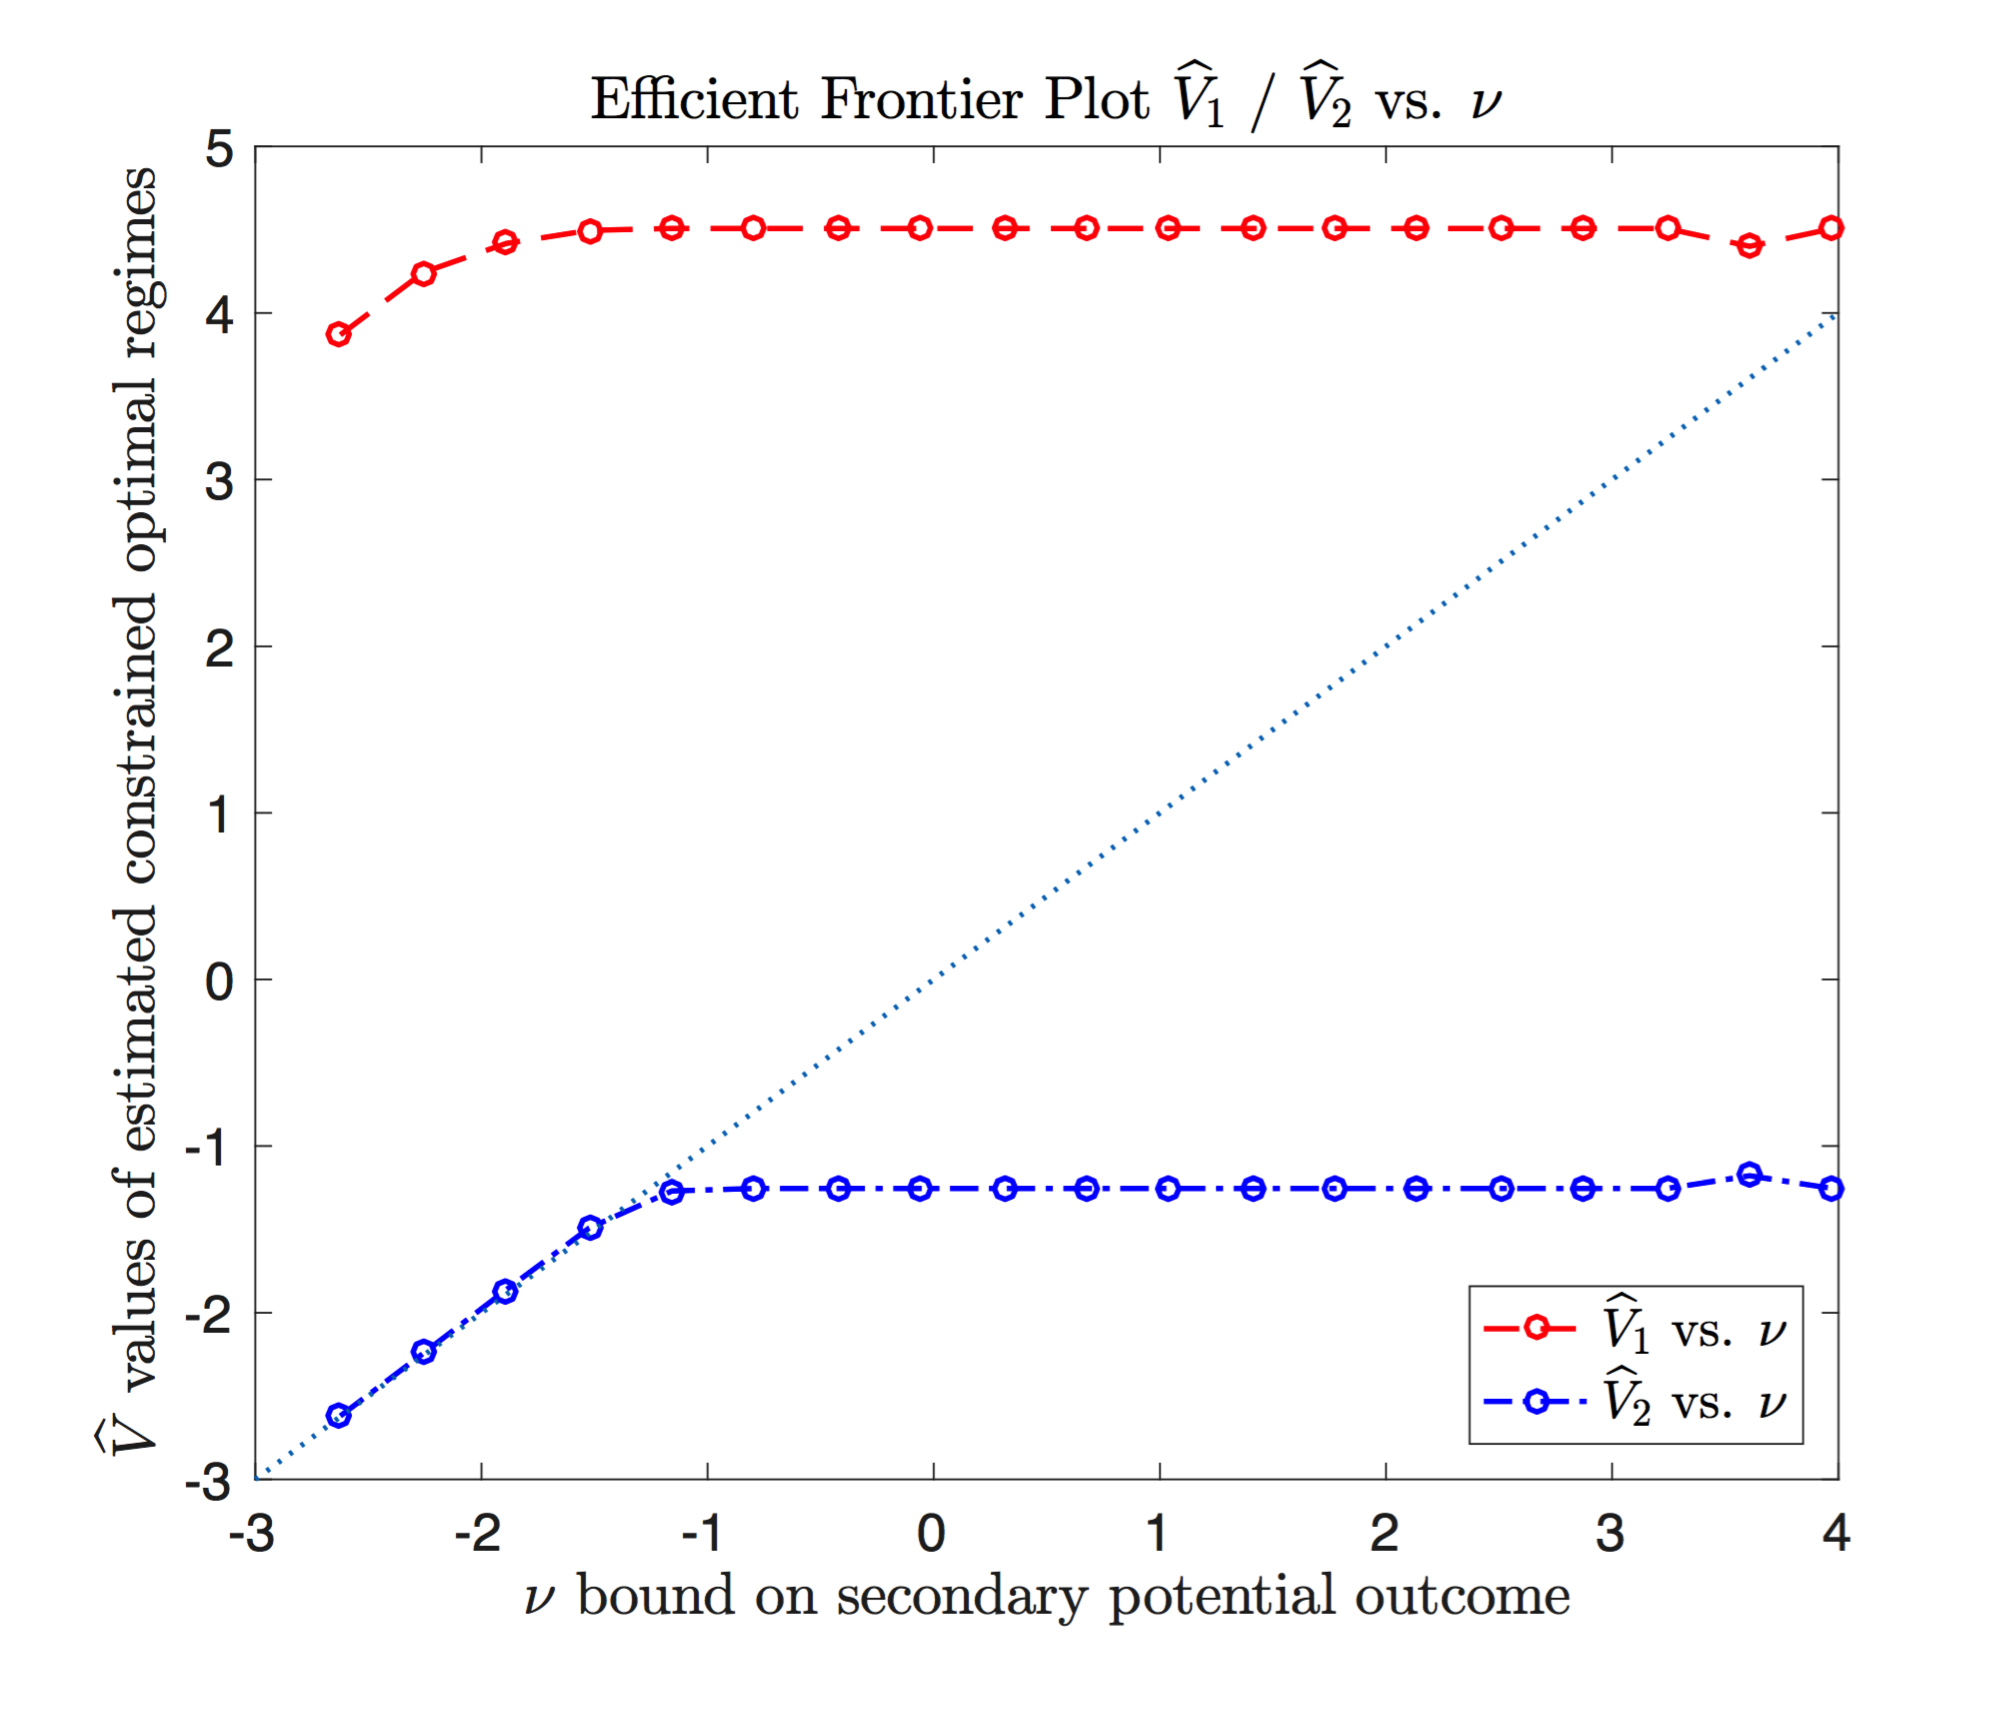
\includegraphics[width=.9\linewidth]{./Chapter-1/figs/efficient_plot2.png}
	\caption{Efficient frontier for estimated constrained optimal regimes for Setting 2.}
	\label{fig:2}
	\justify
X-axis is for the values for the constraints $\nu$; Y-axis is for the values of estimated regimes. Red dashed line is for the values in terms of the primary outcome of interest. Blue dashed line is for the values in terms of the secondary outcome of interest.
\end{figure}
\begin{table}[!htbp]
	\caption {Simulation Result for Setting 3}
	\centering
	{\tt
		\begin{tabular}{rrrrrrrrrr}\hline 
$\nu$  & $\wh{V}_1(\wh{\bs{\theta}}_{\nu})$ & $std(\wh{V}_1)$ & $\wh{V}_2(\wh{\bs{\theta}}_{\nu})$ & $std(\wh{V}_2)$ & $\wh{\theta}_{\nu,1}$ & $std(\wh{\theta}_{\nu,1})$ & $\wh{\theta}_{\nu,2}$ & $std(\wh{\theta}_{\nu,2})$ \\ \hline 
-2.50 &     1.19 &     0.19  &    -2.55 &      0.15 &     -0.05 &      0.10 &      0.99 &      0.01 \\ 
-2.15 &     1.33 &     0.05  &    -2.18 &      0.16 &     -0.24 &      0.07 &      0.97 &      0.02 \\ 
-1.80 &     1.42 &     0.04  &    -1.82 &      0.17 &     -0.39 &      0.06 &      0.92 &      0.03 \\ 
-1.45 &     1.50 &     0.04  &    -1.48 &      0.17 &     -0.51 &      0.06 &      0.86 &      0.03 \\ 
-1.09 &     1.56 &     0.03  &    -1.15 &      0.18 &     -0.60 &      0.05 &      0.79 &      0.04 \\ 
-0.74 &     1.61 &     0.02  &    -0.83 &      0.20 &     -0.69 &      0.05 &      0.72 &      0.04 \\ 
-0.39 &     1.62 &     0.02  &    -0.53 &      0.26 &     -0.75 &      0.06 &      0.66 &      0.06 \\ 
-0.04 &     1.63 &     0.01  &    -0.30 &      0.32 &     -0.79 &      0.06 &      0.61 &      0.07 \\ 
 0.32 &     1.63 &     0.01  &    -0.18 &      0.43 &     -0.81 &      0.07 &      0.58 &      0.10 \\ 
 0.67 &     1.63 &     0.01  &    -0.06 &      0.47 &     -0.82 &      0.08 &      0.55 &      0.11 \\ 
 1.02 &     1.63 &     0.01  &    -0.08 &      0.51 &     -0.82 &      0.08 &      0.55 &      0.12 \\ 
 1.37 &     1.63 &     0.01  &    -0.03 &      0.52 &     -0.83 &      0.08 &      0.54 &      0.13 \\ 
 1.73 &     1.62 &     0.02  &    -0.04 &      0.53 &     -0.83 &      0.08 &      0.54 &      0.13 \\ 
 2.08 &     1.63 &     0.01  &    -0.04 &      0.50 &     -0.83 &      0.08 &      0.54 &      0.12 \\ 
 2.43 &     1.63 &     0.01  &    -0.03 &      0.51 &     -0.83 &      0.08 &      0.54 &      0.12 \\ 
 2.78 &     1.63 &     0.01  &    -0.03 &      0.51 &     -0.83 &      0.08 &      0.54 &      0.12 \\ 
 3.13 &     1.63 &     0.01  &    -0.02 &      0.50 &     -0.83 &      0.08 &      0.54 &      0.12 \\ 
 3.49 &     1.62 &     0.13  &     0.01 &      0.57 &     -0.83 &      0.10 &      0.53 &      0.17 \\ 
 3.84 &     1.63 &     0.01  &     0.00 &      0.52 &     -0.83 &      0.08 &      0.53 &      0.13 \\ \hline 
\end{tabular}

	}
	\justify
	Here, $\nu$ denotes the values of the constraint; $\wh{V}_1(\wh{\bs{\theta}}_{\nu})$ denotes the values of estimated regimes in terms of primary outcome of interest; $std(\wh{V}_1)$ denotes the standard deviation of the estimated regime values in terms of primary outcome of interest; $\wh{V}_2(\wh{\bs{\theta}}_{\nu})$ denotes the values of estimated regimes in terms of secondary outcome of interest; $std(\wh{V}_2)$ denotes the standard deviation of the estimated regime values in terms of secondary outcome of interest; $\wh{\theta}_{\nu,1}$ and $\wh{\theta}_{\nu,2}$ denote the estimated index parameters of the regimes; $std(\wh{\theta}_{\nu,1})$ and $std(\wh{\theta}_{\nu,2})$ denote the standard deviations of those estimated index parameters.	
\end{table} 
\begin{figure}[!htb]
	\centering
	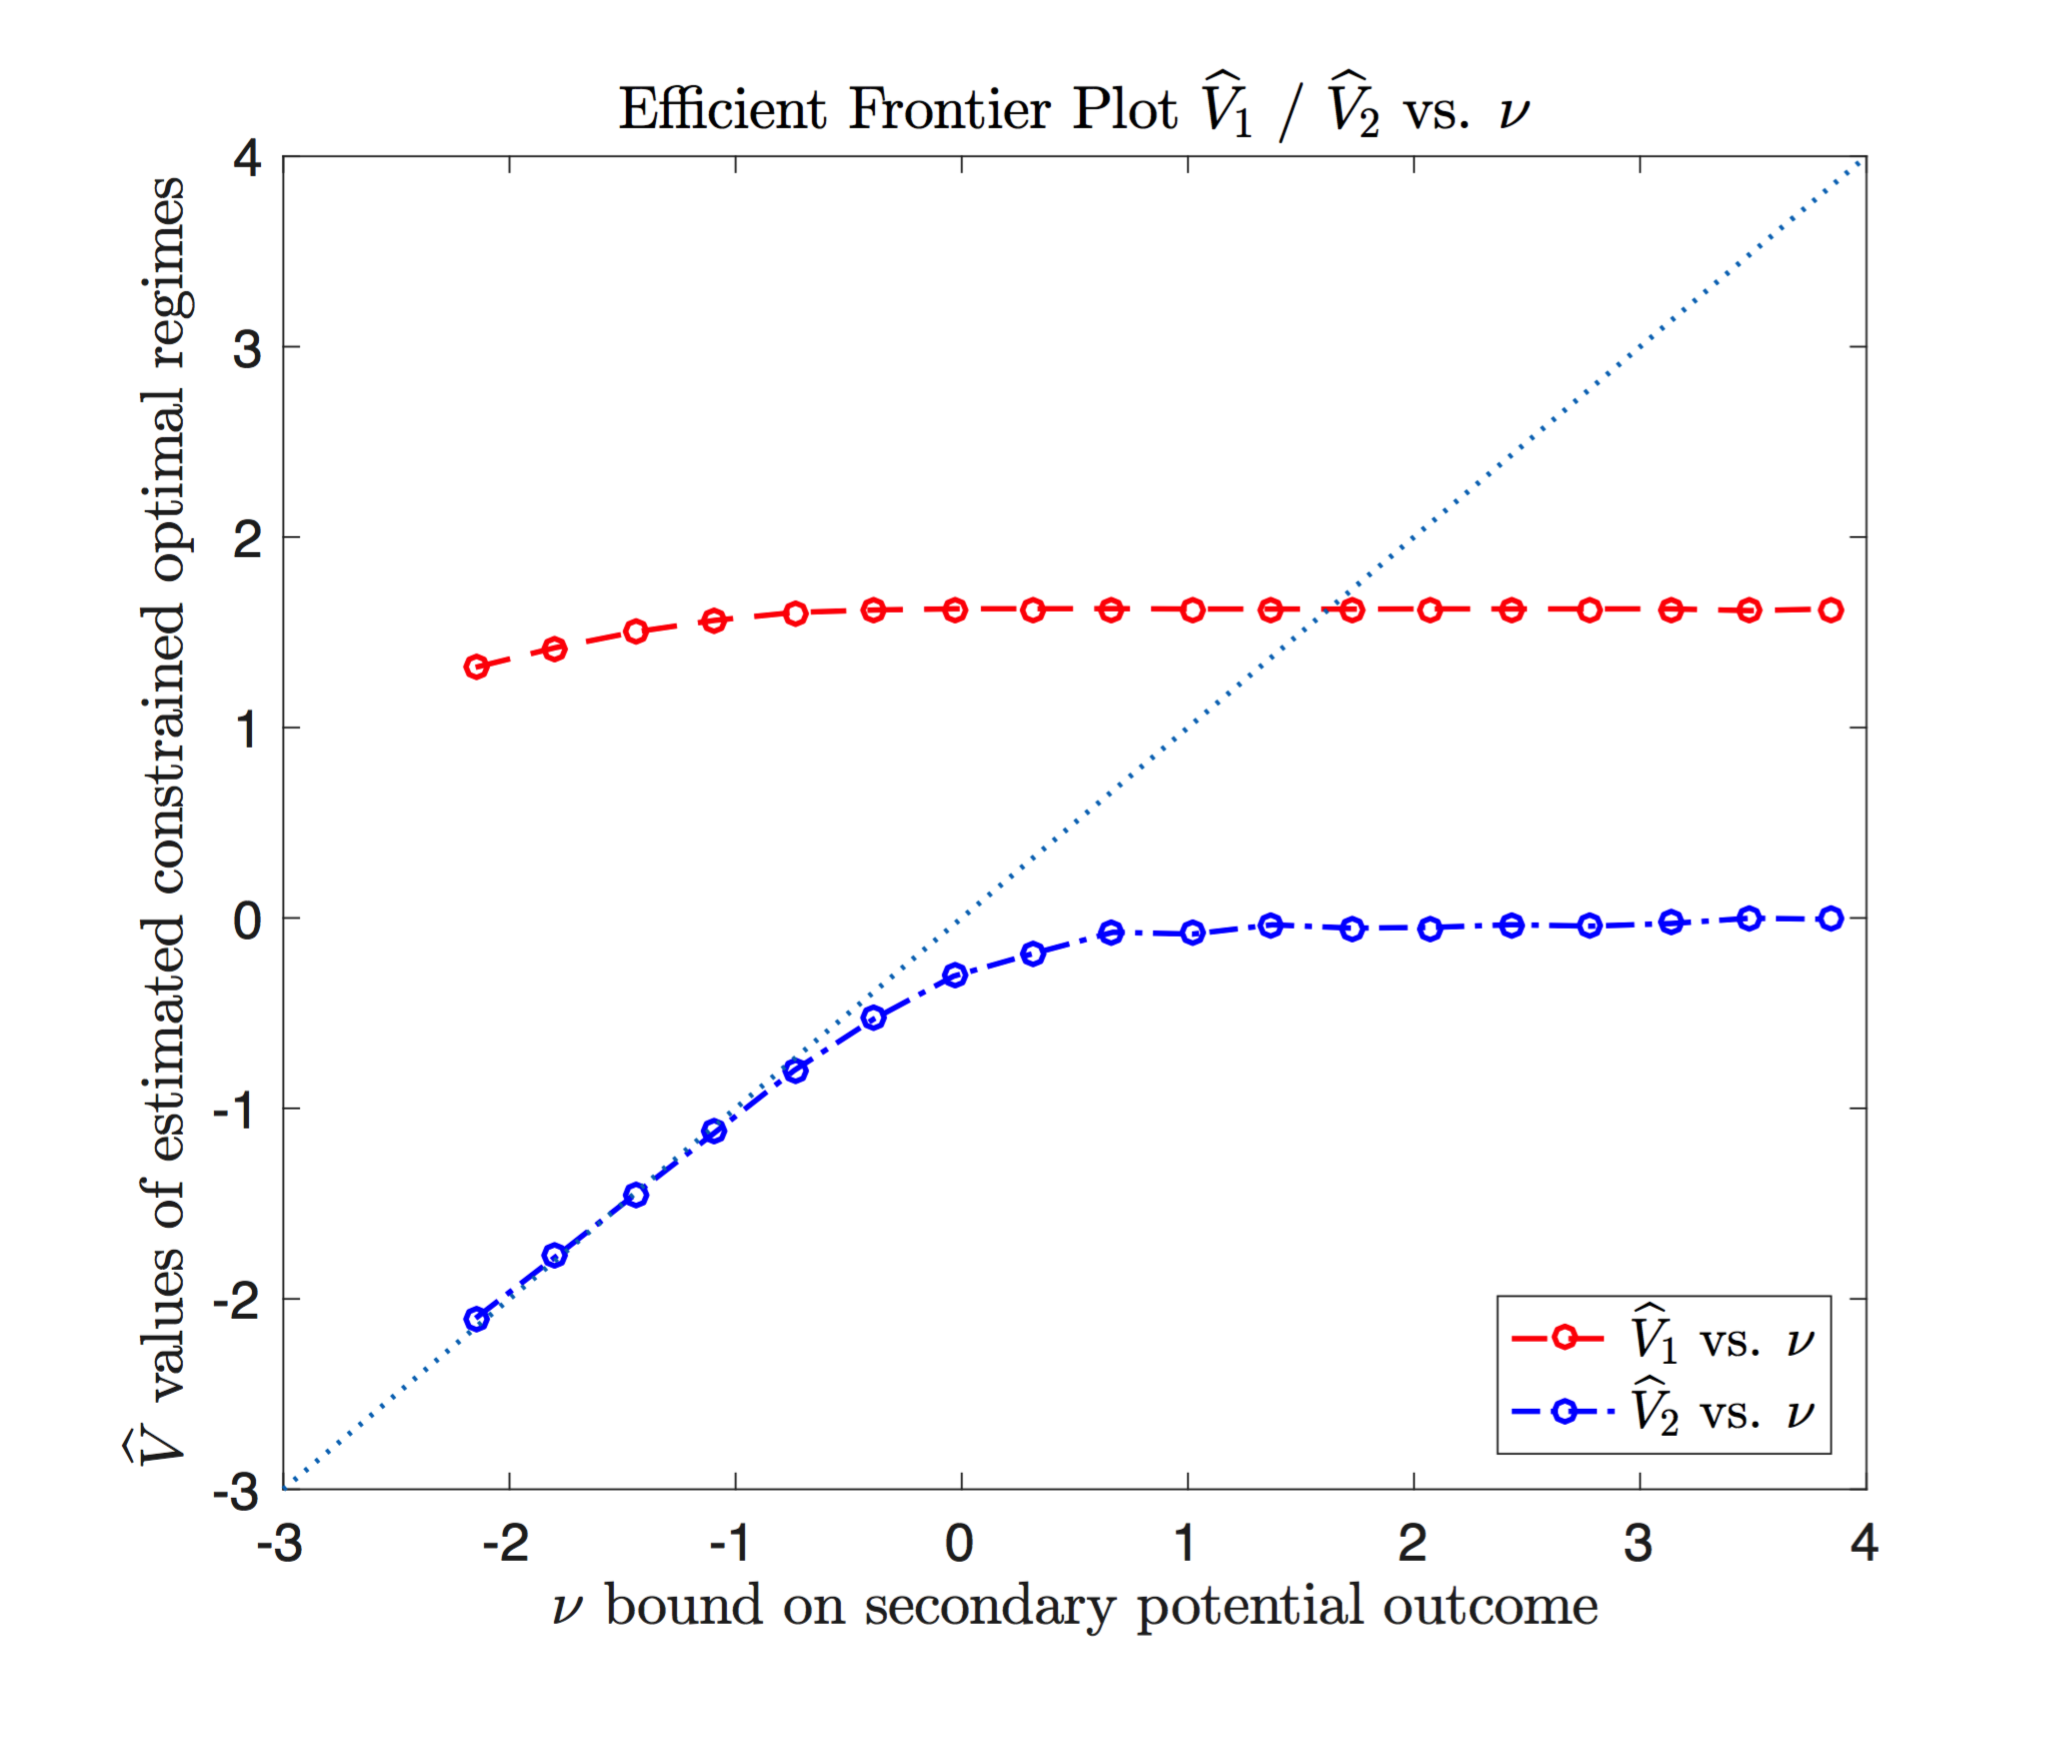
\includegraphics[width=.9\linewidth]{./Chapter-1/figs/efficient_plot3.png}
	\caption{Efficient frontier for estimated constrained optimal regimes for Setting 3.}
	\label{fig:3}
	\justify
X-axis is for the values for the constraints $\nu$; Y-axis is for the values of estimated regimes. Red dashed line is for the values in terms of the primary outcome of interest. Blue dashed line is for the values in terms of the secondary outcome of interest.
\end{figure}
\begin{table}[!htbp]
	\caption {Simulation Result for Setting 4}
	\centering
	{\tt
		\begin{tabular}{rrrrrrrrrr}\hline 
$\nu$  & $\wh{V}_1(\wh{\bs{\theta}}_{\nu})$ & $std(\wh{V}_1)$ & $\wh{V}_2(\wh{\bs{\theta}}_{\nu})$ & $std(\wh{V}_2)$ & $\wh{\theta}_{\nu,1}$ & $std(\wh{\theta}_{\nu,1})$ & $\wh{\theta}_{\nu,2}$ & $std(\wh{\theta}_{\nu,2})$ \\ \hline 
%4 &      NaN &      NaN &      NaN  &      NaN &       NaN &       NaN &       NaN &       NaN &       NaN \\ 
%4 &      NaN &      NaN &      NaN  &      NaN &       NaN &       NaN &       NaN &       NaN &       NaN \\ 
%4 &    -1.81 &      NaN &      NaN  &      NaN &       NaN &       NaN &       NaN &       NaN &       NaN \\ 
-1.57 &     1.62 &     0.01  &    -1.82 &      0.03 &      0.14 &      0.12 &     -0.98 &      0.02 \\ 
-1.32 &     1.62 &     0.02  &    -1.81 &      0.04 &      0.14 &      0.13 &     -0.98 &      0.02 \\ 
-1.08 &     1.62 &     0.02  &    -1.82 &      0.03 &      0.15 &      0.13 &     -0.98 &      0.02 \\ 
-0.84 &     1.62 &     0.02  &    -1.81 &      0.04 &      0.14 &      0.13 &     -0.98 &      0.02 \\ 
-0.59 &     1.62 &     0.02  &    -1.81 &      0.04 &      0.14 &      0.13 &     -0.98 &      0.02 \\ 
-0.35 &     1.62 &     0.02  &    -1.81 &      0.04 &      0.14 &      0.13 &     -0.98 &      0.02 \\ 
-0.10 &     1.62 &     0.02  &    -1.81 &      0.04 &      0.14 &      0.13 &     -0.98 &      0.02 \\ 
 0.14 &     1.62 &     0.02  &    -1.81 &      0.04 &      0.14 &      0.13 &     -0.98 &      0.02 \\ 
 0.38 &     1.62 &     0.02  &    -1.81 &      0.04 &      0.14 &      0.13 &     -0.98 &      0.02 \\ 
 0.63 &     1.62 &     0.02  &    -1.81 &      0.04 &      0.14 &      0.13 &     -0.98 &      0.02 \\ 
 0.87 &     1.62 &     0.02  &    -1.81 &      0.04 &      0.14 &      0.14 &     -0.98 &      0.02 \\ 
 1.11 &     1.62 &     0.02  &    -1.81 &      0.04 &      0.14 &      0.13 &     -0.98 &      0.02 \\ 
 1.36 &     1.62 &     0.02  &    -1.81 &      0.04 &      0.15 &      0.13 &     -0.98 &      0.02 \\ 
 1.60 &     1.62 &     0.02  &    -1.81 &      0.04 &      0.14 &      0.13 &     -0.98 &      0.02 \\ 
 1.84 &     1.62 &     0.02  &    -1.81 &      0.04 &      0.14 &      0.13 &     -0.98 &      0.02 \\ 
 2.09 &     1.62 &     0.02  &    -1.81 &      0.04 &      0.14 &      0.13 &     -0.98 &      0.02 \\ 
 2.33 &     1.62 &     0.02  &    -1.81 &      0.04 &      0.14 &      0.13 &     -0.98 &      0.02 \\ 
 2.57 &     1.62 &     0.02  &    -1.81 &      0.04 &      0.14 &      0.13 &     -0.98 &      0.02 \\ 
 2.82 &     1.62 &     0.02  &    -1.81 &      0.04 &      0.14 &      0.13 &     -0.98 &      0.02 \\ \hline 
\end{tabular}

	}
	\justify
	Here, $\nu$ denotes the values of the constraint; $\wh{V}_1(\wh{\bs{\theta}}_{\nu})$ denotes the values of estimated regimes in terms of primary outcome of interest; $std(\wh{V}_1)$ denotes the standard deviation of the estimated regime values in terms of primary outcome of interest; $\wh{V}_2(\wh{\bs{\theta}}_{\nu})$ denotes the values of estimated regimes in terms of secondary outcome of interest; $std(\wh{V}_2)$ denotes the standard deviation of the estimated regime values in terms of secondary outcome of interest; $\wh{\theta}_{\nu,1}$ and $\wh{\theta}_{\nu,2}$ denote the estimated index parameters of the regimes; $std(\wh{\theta}_{\nu,1})$ and $std(\wh{\theta}_{\nu,2})$ denote the standard deviations of those estimated index parameters.	
\end{table} 
\begin{figure}[!htb]
	\centering
	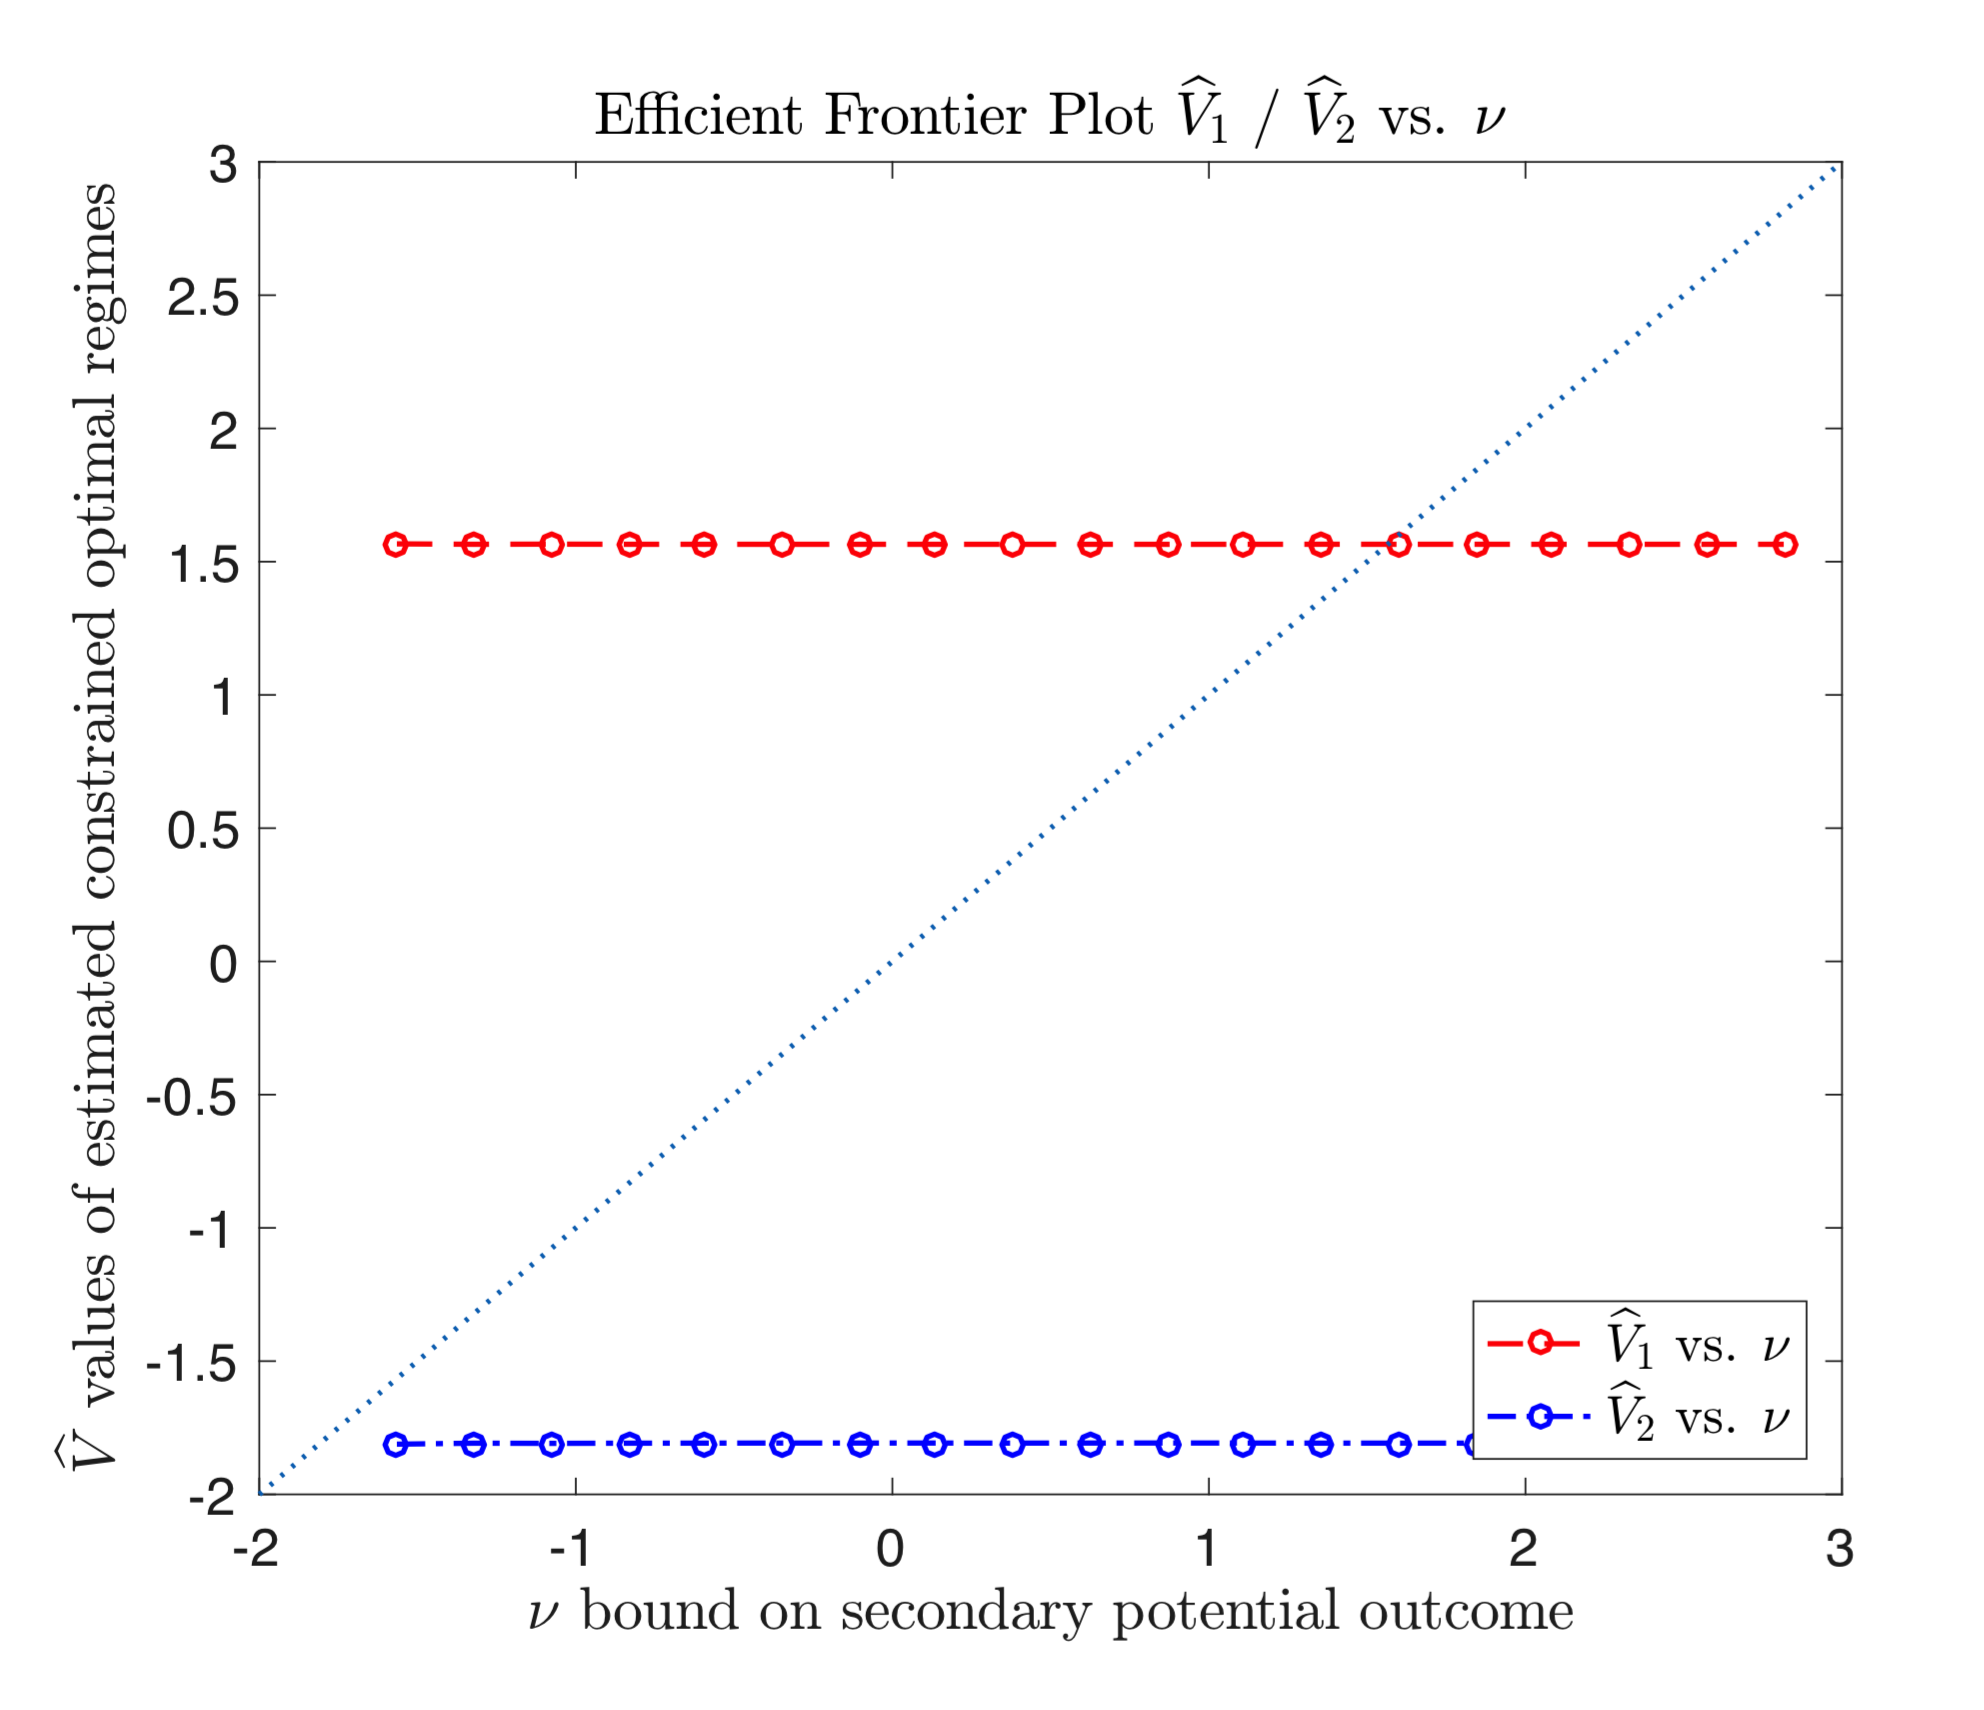
\includegraphics[width=.9\linewidth]{./Chapter-1/figs/efficient_plot4.png}
	\caption{Efficient frontier for estimated constrained optimal regimes for Setting 4.}
	\label{fig:4}
	\justify
X-axis is for the values for the constraints $\nu$; Y-axis is for the values of estimated regimes. Red dashed line is for the values in terms of the primary outcome of interest. Blue dashed line is for the values in terms of the secondary outcome of interest.
\end{figure}
\begin{table}[!htbp]
	\caption {Simulation Result for Setting 5}
	\centering
	{\tt
		\begin{tabular}{rrrrrrrrrr}\hline 
$\nu$  & $\wh{V}_1(\wh{\bs{\theta}}_{\nu})$ & $std(\wh{V}_1)$ & $\wh{V}_2(\wh{\bs{\theta}}_{\nu})$ & $std(\wh{V}_2)$ & $\wh{\theta}_{\nu,1}$ & $std(\wh{\theta}_{\nu,1})$ & $\wh{\theta}_{\nu,2}$ & $std(\wh{\theta}_{\nu,2})$ \\ \hline 
%5 &      NaN &      NaN &      NaN  &      NaN &       NaN &       NaN &       NaN &       NaN &       NaN \\ 
%5 &      NaN &      NaN &      NaN  &      NaN &       NaN &       NaN &       NaN &       NaN &       NaN \\ 
%5 &    -2.94 &      NaN &      NaN  &      NaN &       NaN &       NaN &       NaN &       NaN &       NaN \\ 
-2.58 &     0.64 &     0.04  &    -2.62 &      0.15 &      0.80 &      0.09 &     -0.59 &      0.10 \\ 
-2.22 &     0.70 &     0.03  &    -2.29 &      0.20 &      0.90 &      0.07 &     -0.42 &      0.11 \\ 
-1.85 &     0.74 &     0.04  &    -1.97 &      0.24 &      0.95 &      0.07 &     -0.27 &      0.12 \\ 
-1.49 &     0.76 &     0.04  &    -1.68 &      0.33 &      0.98 &      0.05 &     -0.16 &      0.14 \\ 
-1.13 &     0.79 &     0.04  &    -1.37 &      0.39 &      0.99 &      0.04 &     -0.05 &      0.15 \\ 
-0.77 &     0.80 &     0.04  &    -1.12 &      0.46 &      0.98 &      0.03 &      0.04 &      0.17 \\ 
-0.40 &     0.80 &     0.05  &    -0.91 &      0.59 &      0.97 &      0.06 &      0.10 &      0.22 \\ 
-0.04 &     0.80 &     0.05  &    -0.67 &      0.63 &      0.95 &      0.13 &      0.18 &      0.22 \\ 
 0.32 &     0.80 &     0.06  &    -0.44 &      0.75 &      0.92 &      0.15 &      0.24 &      0.27 \\ 
 0.68 &     0.80 &     0.06  &    -0.23 &      0.82 &      0.91 &      0.15 &      0.29 &      0.26 \\ 
 1.05 &     0.80 &     0.07  &    -0.08 &      0.93 &      0.88 &      0.19 &      0.33 &      0.28 \\ 
 1.41 &     0.80 &     0.07  &     0.10 &      0.97 &      0.86 &      0.20 &      0.37 &      0.28 \\ 
 1.77 &     0.80 &     0.05  &     0.15 &      1.04 &      0.86 &      0.17 &      0.39 &      0.29 \\ 
 2.13 &     0.80 &     0.05  &     0.24 &      1.10 &      0.84 &      0.18 &      0.41 &      0.30 \\ 
 2.50 &     0.80 &     0.05  &     0.29 &      1.14 &      0.83 &      0.19 &      0.42 &      0.31 \\ 
 2.86 &     0.80 &     0.03  &     0.38 &      1.20 &      0.82 &      0.17 &      0.44 &      0.31 \\ 
 3.22 &     0.80 &     0.03  &     0.44 &      1.21 &      0.81 &      0.19 &      0.46 &      0.31 \\ 
 3.58 &     0.80 &     0.03  &     0.34 &      1.19 &      0.83 &      0.18 &      0.44 &      0.31 \\ 
 3.94 &     0.80 &     0.04  &     0.48 &      1.29 &      0.80 &      0.22 &      0.46 &      0.32 \\ \hline 
\end{tabular}

	}
	\justify
	Here, $\nu$ denotes the values of the constraint; $\wh{V}_1(\wh{\bs{\theta}}_{\nu})$ denotes the values of estimated regimes in terms of primary outcome of interest; $std(\wh{V}_1)$ denotes the standard deviation of the estimated regime values in terms of primary outcome of interest; $\wh{V}_2(\wh{\bs{\theta}}_{\nu})$ denotes the values of estimated regimes in terms of secondary outcome of interest; $std(\wh{V}_2)$ denotes the standard deviation of the estimated regime values in terms of secondary outcome of interest; $\wh{\theta}_{\nu,1}$ and $\wh{\theta}_{\nu,2}$ denote the estimated index parameters of the regimes; $std(\wh{\theta}_{\nu,1})$ and $std(\wh{\theta}_{\nu,2})$ denote the standard deviations of those estimated index parameters.	
\end{table} 
\begin{figure}[!htb]
	\centering
	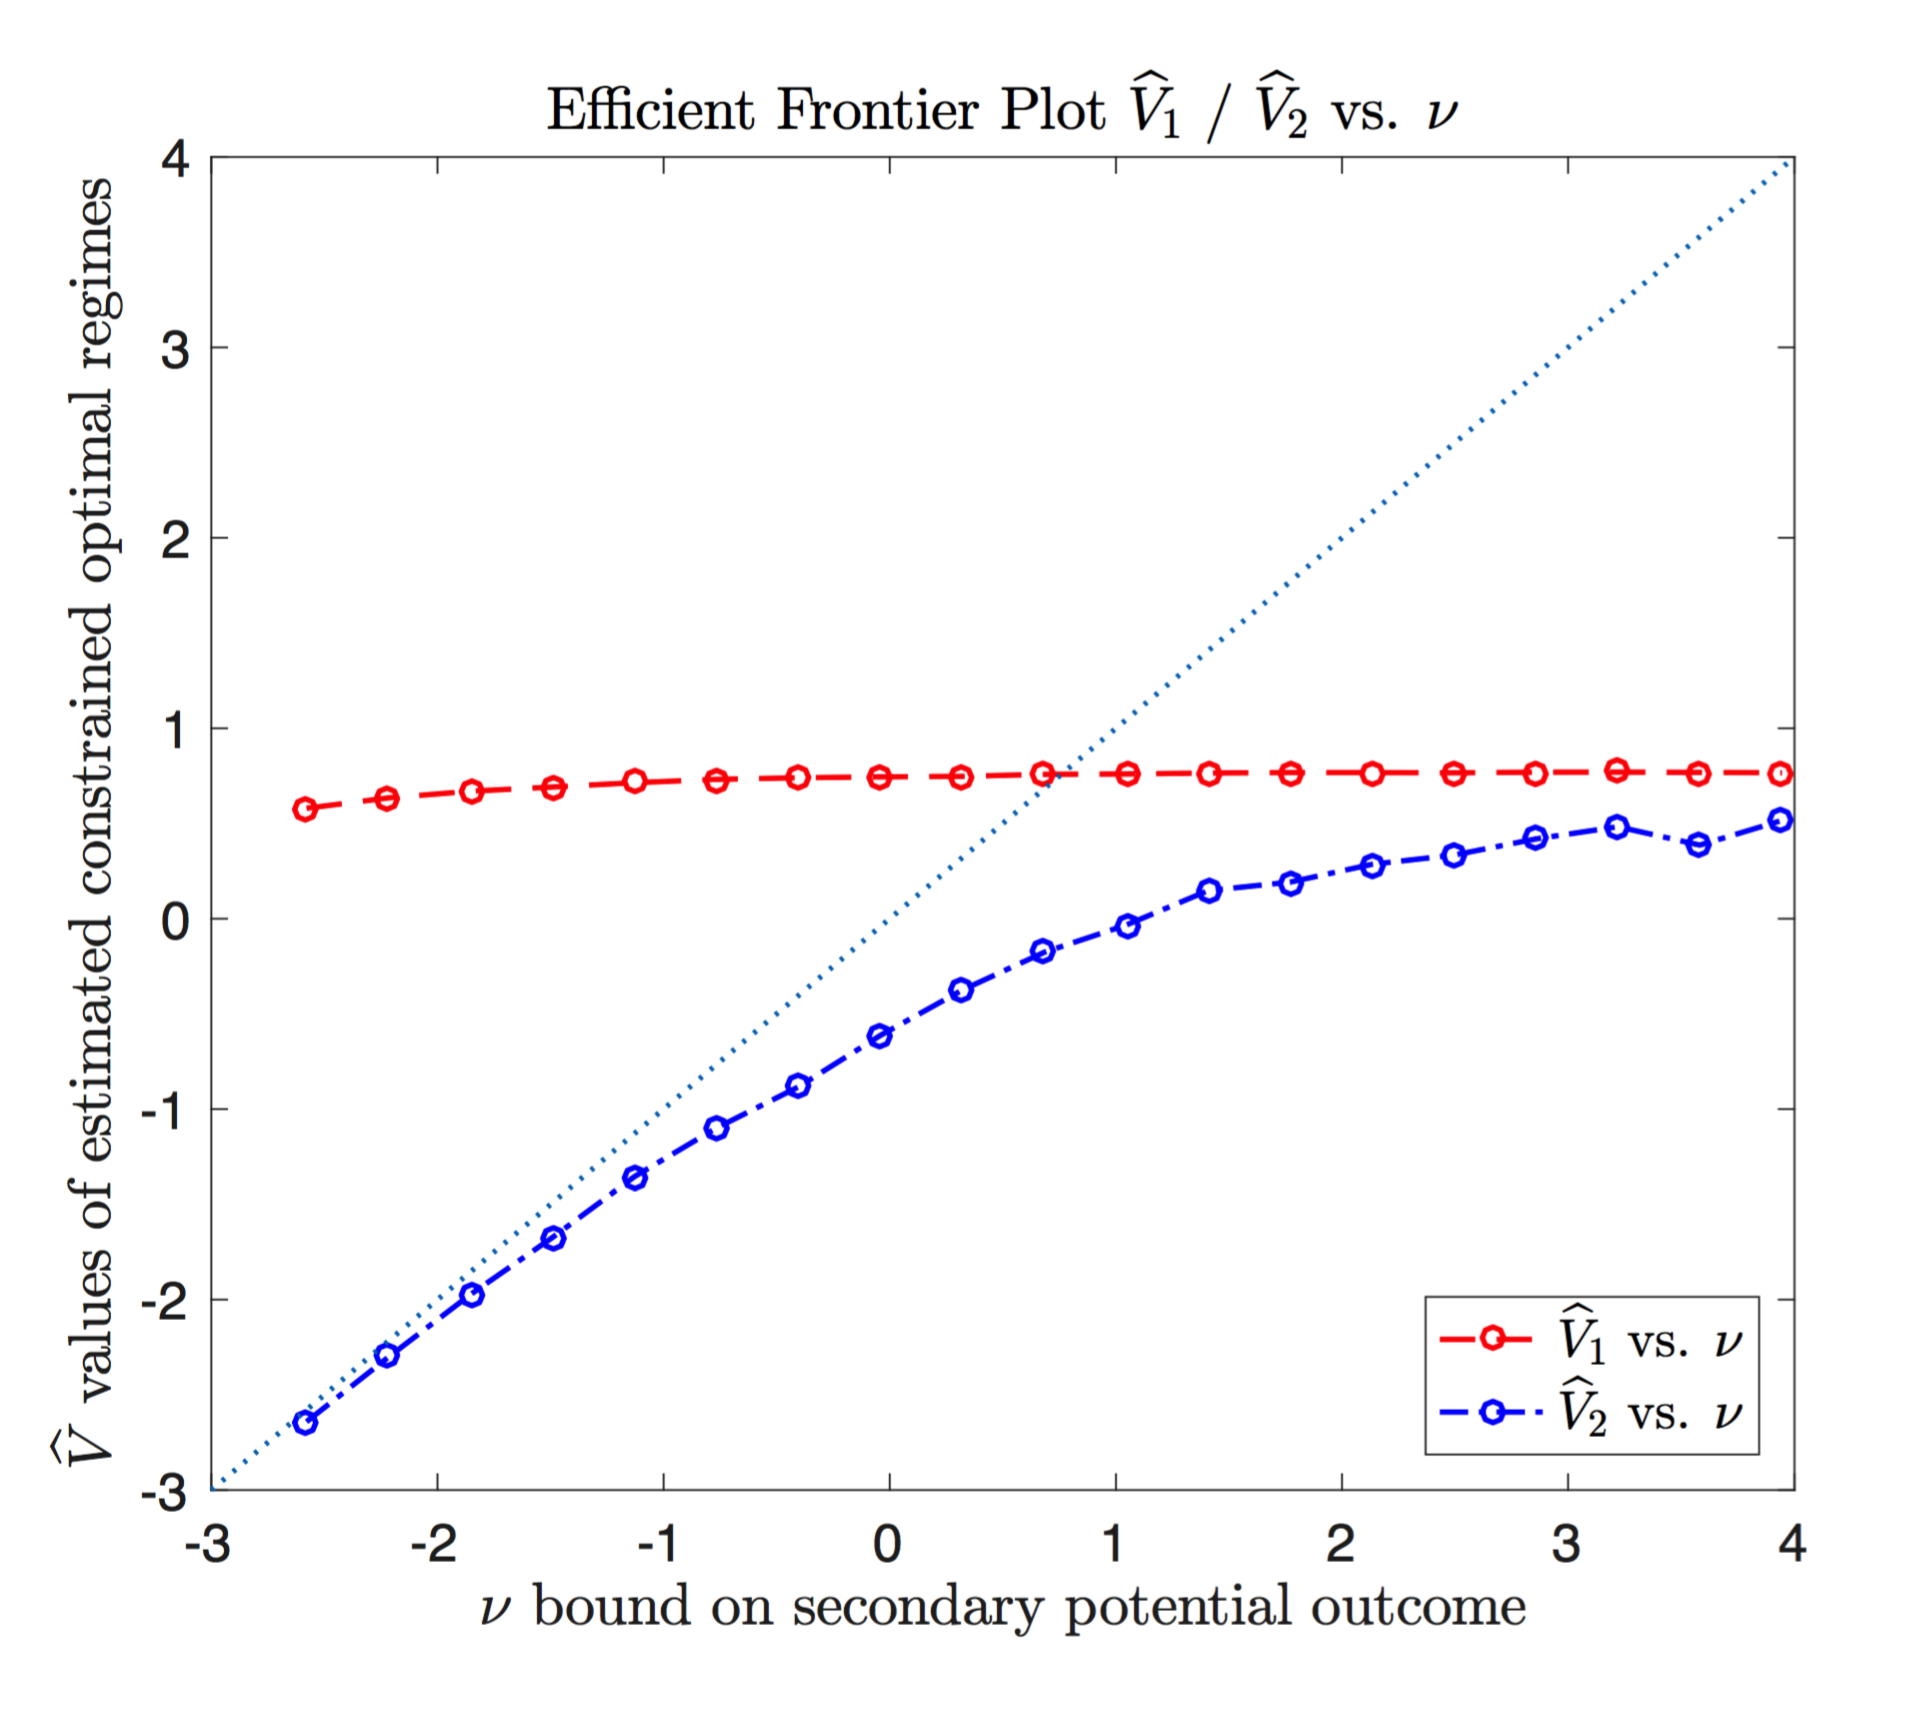
\includegraphics[width=.9\linewidth]{./Chapter-1/figs/efficient_plot5.png}
	\caption{Efficient frontier for estimated constrained optimal regimes for Setting 5.}
	\label{fig:5}
	\justify
X-axis is for the values for the constraints $\nu$; Y-axis is for the values of estimated regimes. Red dashed line is for the values in terms of the primary outcome of interest. Blue dashed line is for the values in terms of the secondary outcome of interest.
\end{figure}
\begin{table}[!htbp]
	\caption {Simulation Result for Setting 6}
	\centering
	{\tt
		\begin{tabular}{rrrrrrrrrr}\hline 
$\nu$  & $\wh{V}_1(\wh{\bs{\theta}}_{\nu})$ & $std(\wh{V}_1)$ & $\wh{V}_2(\wh{\bs{\theta}}_{\nu})$ & $std(\wh{V}_2)$ & $\wh{\theta}_{\nu,1}$ & $std(\wh{\theta}_{\nu,1})$ & $\wh{\theta}_{\nu,2}$ & $std(\wh{\theta}_{\nu,2})$ \\ \hline 
%6 &      NaN &      NaN &      NaN  &      NaN &       NaN &       NaN &       NaN &       NaN &       NaN \\ 
%6 &      NaN &      NaN &      NaN  &      NaN &       NaN &       NaN &       NaN &       NaN &       NaN \\ 
%6 &    -0.61 &      NaN &      NaN  &      NaN &       NaN &       NaN &       NaN &       NaN &       NaN \\ 
-0.50 &     0.59 &     0.11  &    -0.55 &      0.41 &     -0.83 &      0.31 &     -0.44 &      0.13 \\ 
-0.38 &     0.73 &     0.08  &    -0.36 &      0.07 &     -0.96 &      0.03 &     -0.26 &      0.11 \\ 
-0.26 &     0.85 &     0.07  &    -0.25 &      0.08 &     -0.99 &      0.01 &     -0.11 &      0.10 \\ 
-0.14 &     0.94 &     0.06  &    -0.13 &      0.09 &     -1.00 &      0.01 &      0.02 &      0.09 \\ 
-0.03 &     1.01 &     0.05  &    -0.00 &      0.09 &     -0.99 &      0.01 &      0.15 &      0.08 \\ 
 0.09 &     1.07 &     0.04  &     0.12 &      0.09 &     -0.96 &      0.02 &      0.26 &      0.08 \\ 
 0.21 &     1.12 &     0.03  &     0.24 &      0.09 &     -0.93 &      0.03 &      0.36 &      0.07 \\ 
 0.33 &     1.15 &     0.14  &     0.36 &      0.09 &     -0.87 &      0.17 &      0.45 &      0.13 \\ 
 0.44 &     1.18 &     0.14  &     0.48 &      0.08 &     -0.82 &      0.17 &      0.54 &      0.13 \\ 
 0.56 &     1.21 &     0.14  &     0.60 &      0.09 &     -0.76 &      0.17 &      0.62 &      0.13 \\ 
 0.68 &     1.20 &     0.25  &     0.71 &      0.09 &     -0.65 &      0.30 &      0.67 &      0.22 \\ 
 0.80 &     1.23 &     0.19  &     0.80 &      0.09 &     -0.61 &      0.23 &      0.74 &      0.17 \\ 
 0.91 &     1.23 &     0.18  &     0.88 &      0.10 &     -0.56 &      0.23 &      0.78 &      0.16 \\ 
 1.03 &     1.25 &     0.09  &     0.92 &      0.12 &     -0.54 &      0.15 &      0.82 &      0.10 \\ 
 1.15 &     1.26 &     0.01  &     0.95 &      0.14 &     -0.52 &      0.12 &      0.84 &      0.08 \\ 
 1.27 &     1.25 &     0.01  &     0.96 &      0.15 &     -0.51 &      0.13 &      0.85 &      0.08 \\ 
 1.38 &     1.25 &     0.01  &     0.96 &      0.15 &     -0.51 &      0.12 &      0.85 &      0.08 \\ 
 1.50 &     1.25 &     0.01  &     0.96 &      0.15 &     -0.51 &      0.13 &      0.85 &      0.08 \\ 
 1.62 &     1.25 &     0.01  &     0.96 &      0.15 &     -0.51 &      0.13 &      0.85 &      0.08 \\ \hline 
\end{tabular}

	}
	\justify
	Here, $\nu$ denotes the values of the constraint; $\wh{V}_1(\wh{\bs{\theta}}_{\nu})$ denotes the values of estimated regimes in terms of primary outcome of interest; $std(\wh{V}_1)$ denotes the standard deviation of the estimated regime values in terms of primary outcome of interest; $\wh{V}_2(\wh{\bs{\theta}}_{\nu})$ denotes the values of estimated regimes in terms of secondary outcome of interest; $std(\wh{V}_2)$ denotes the standard deviation of the estimated regime values in terms of secondary outcome of interest; $\wh{\theta}_{\nu,1}$ and $\wh{\theta}_{\nu,2}$ denote the estimated index parameters of the regimes; $std(\wh{\theta}_{\nu,1})$ and $std(\wh{\theta}_{\nu,2})$ denote the standard deviations of those estimated index parameters.	
\end{table} 
\begin{figure}[!htb]
	\centering
	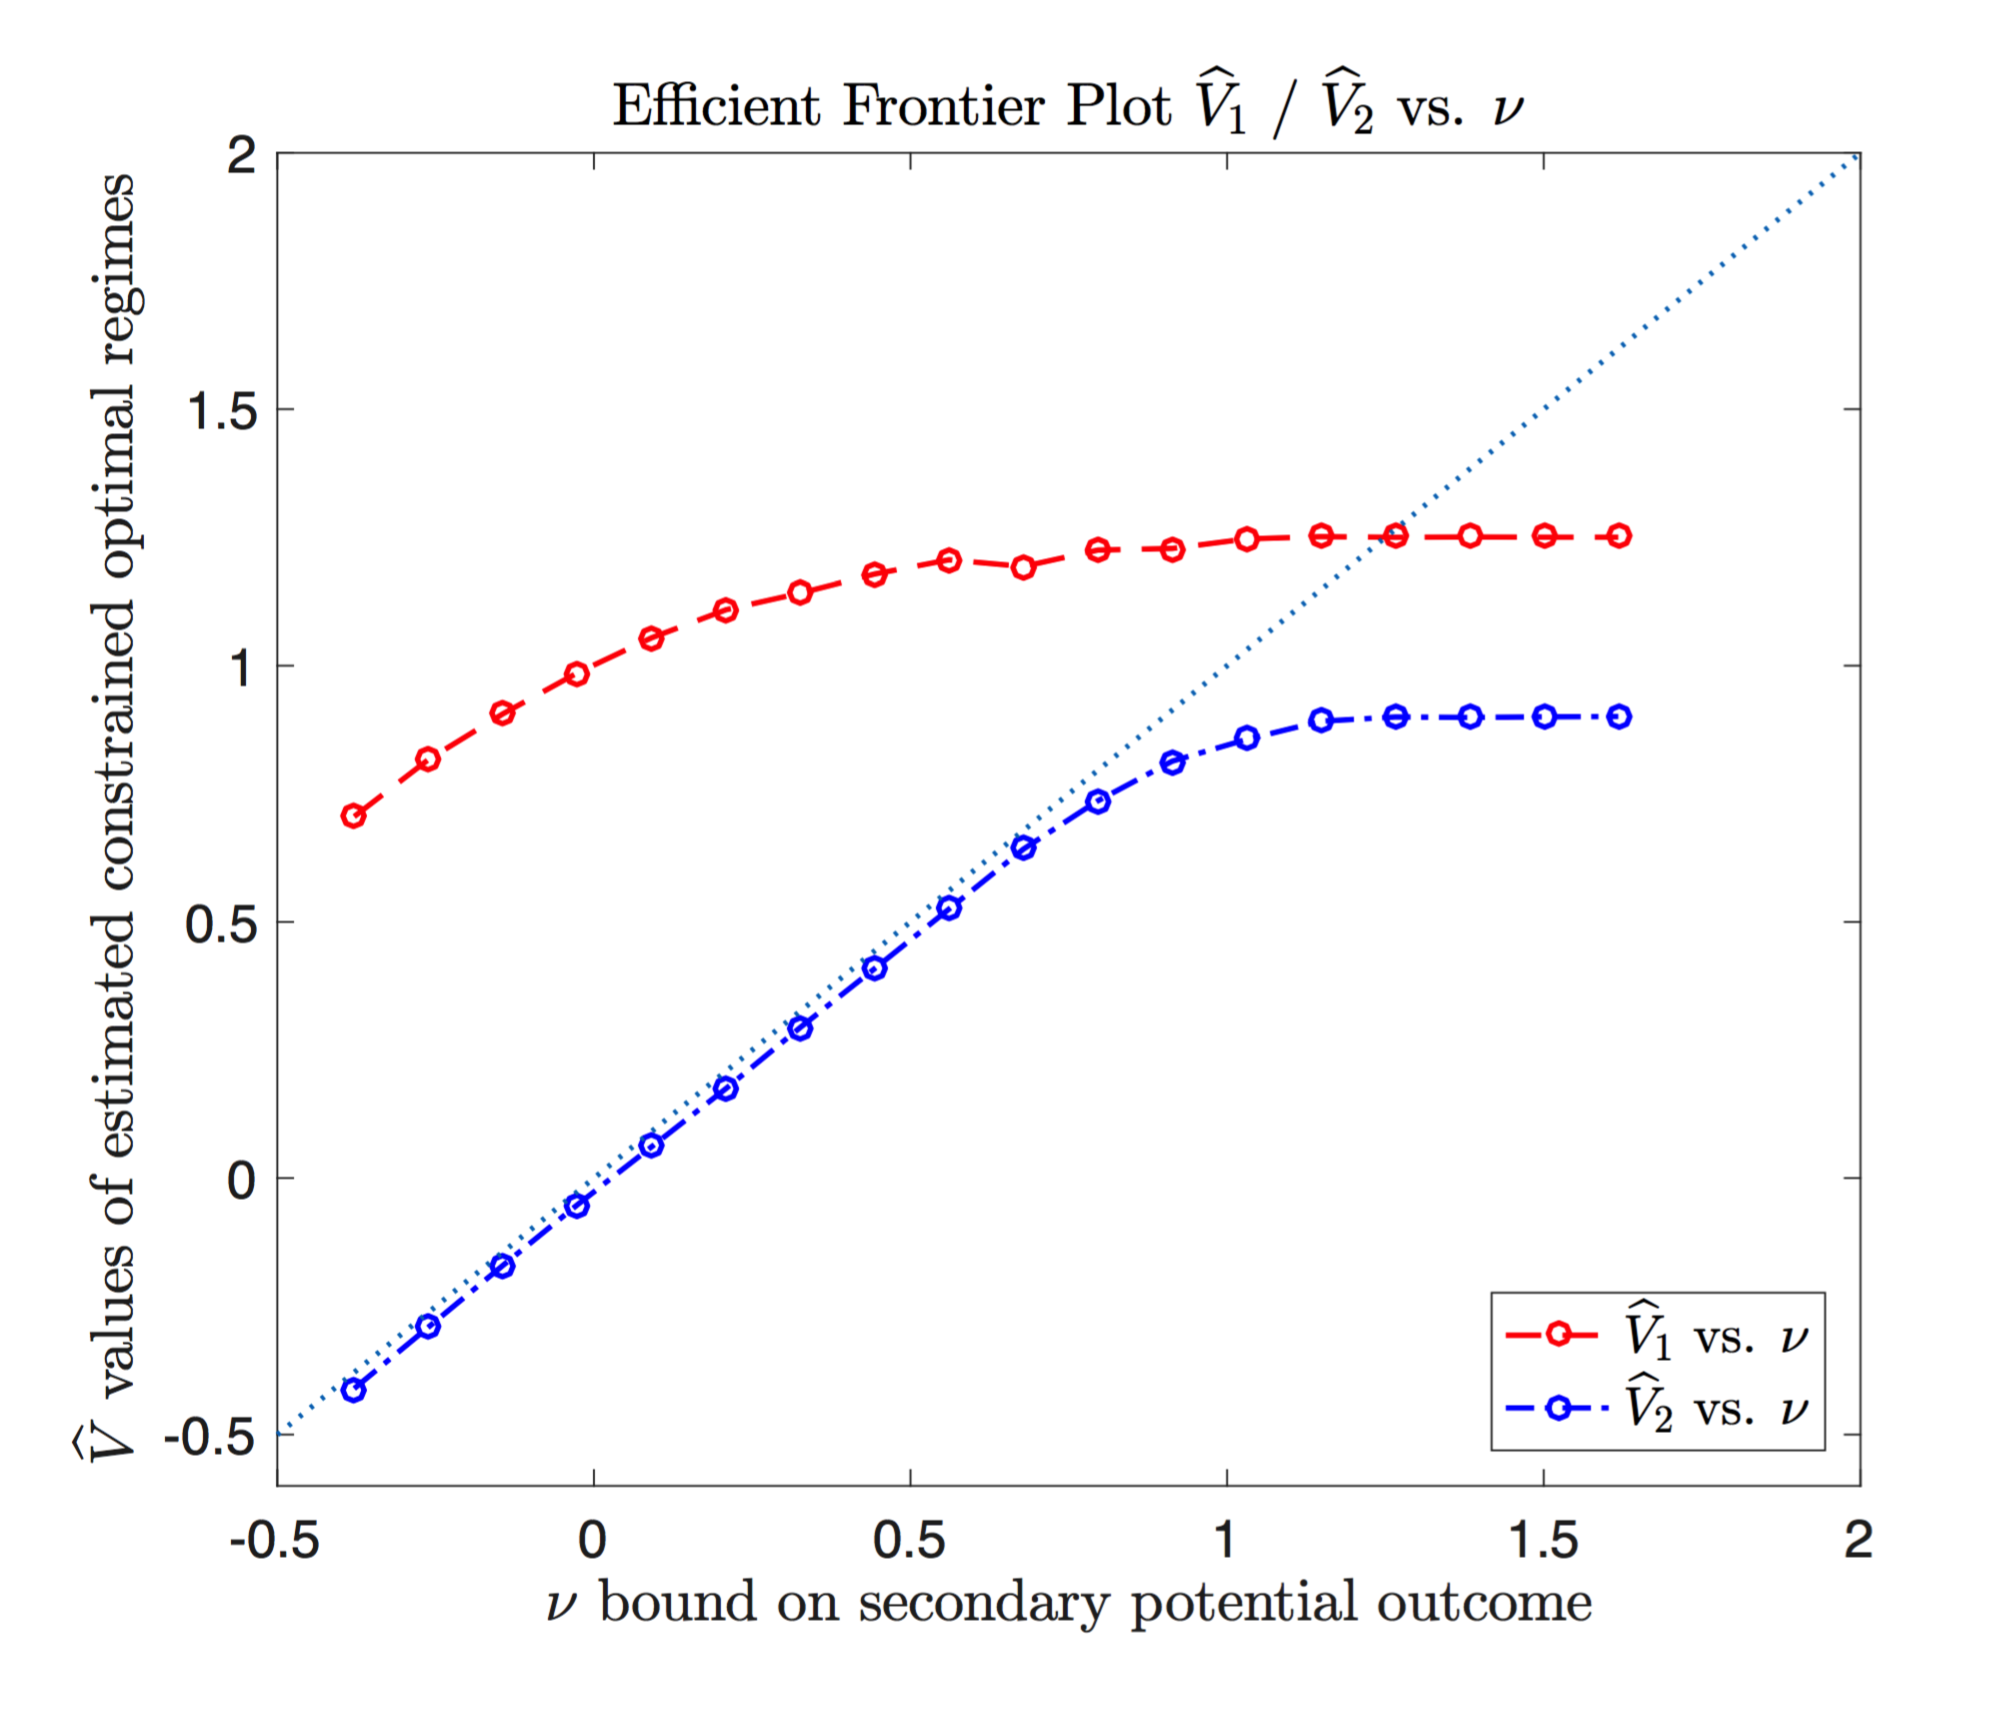
\includegraphics[width=.9\linewidth]{./Chapter-1/figs/efficient_plot6.png}
	\caption{Efficient frontier for estimated constrained optimal regimes for Setting 6.}
	\label{fig:6}
	\justify
X-axis is for the values for the constraints $\nu$; Y-axis is for the values of estimated regimes. Red dashed line is for the values in terms of the primary outcome of interest. Blue dashed line is for the values in terms of the secondary outcome of interest.
\end{figure}
\begin{table}[!htbp]
	\caption {Simulation Result for Setting 7}
	\centering
	{\tt
		\begin{tabular}{rrrrrrrrrr}\hline 
$\nu$  & $\wh{V}_1(\wh{\bs{\theta}}_{\nu})$ & $std(\wh{V}_1)$ & $\wh{V}_2(\wh{\bs{\theta}}_{\nu})$ & $std(\wh{V}_2)$ & $\wh{\theta}_{\nu,1}$ & $std(\wh{\theta}_{\nu,1})$ & $\wh{\theta}_{\nu,2}$ & $std(\wh{\theta}_{\nu,2})$ \\ \hline 
%7 &      NaN &      NaN &      NaN  &      NaN &       NaN &       NaN &       NaN &       NaN &       NaN \\ 
%7 &      NaN &      NaN &      NaN  &      NaN &       NaN &       NaN &       NaN &       NaN &       NaN \\ 
%7 &    -3.42 &      NaN &      NaN  &      NaN &       NaN &       NaN &       NaN &       NaN &       NaN \\ 
-3.01 &     1.12 &     0.01  &    -3.28 &      0.12 &     -0.70 &      0.10 &      0.70 &      0.10 \\ 
-2.60 &     1.12 &     0.01  &    -3.27 &      0.14 &     -0.69 &      0.11 &      0.71 &      0.10 \\ 
-2.19 &     1.12 &     0.01  &    -3.26 &      0.16 &     -0.69 &      0.11 &      0.71 &      0.11 \\ 
-1.77 &     1.12 &     0.01  &    -3.26 &      0.17 &     -0.69 &      0.11 &      0.71 &      0.11 \\ 
-1.36 &     1.12 &     0.01  &    -3.27 &      0.14 &     -0.69 &      0.11 &      0.70 &      0.11 \\ 
-0.95 &     1.12 &     0.01  &    -3.26 &      0.17 &     -0.69 &      0.11 &      0.71 &      0.11 \\ 
-0.54 &     1.12 &     0.01  &    -3.26 &      0.17 &     -0.69 &      0.11 &      0.71 &      0.11 \\ 
-0.12 &     1.12 &     0.01  &    -3.26 &      0.17 &     -0.69 &      0.11 &      0.71 &      0.11 \\ 
 0.29 &     1.12 &     0.01  &    -3.25 &      0.17 &     -0.69 &      0.11 &      0.71 &      0.11 \\ 
 0.70 &     1.12 &     0.01  &    -3.26 &      0.17 &     -0.69 &      0.12 &      0.71 &      0.11 \\ 
 1.11 &     1.12 &     0.01  &    -3.25 &      0.17 &     -0.68 &      0.11 &      0.71 &      0.11 \\ 
 1.53 &     1.12 &     0.01  &    -3.26 &      0.17 &     -0.69 &      0.11 &      0.71 &      0.11 \\ 
 1.94 &     1.12 &     0.01  &    -3.26 &      0.17 &     -0.69 &      0.11 &      0.71 &      0.11 \\ 
 2.35 &     1.12 &     0.01  &    -3.26 &      0.17 &     -0.69 &      0.11 &      0.71 &      0.11 \\ 
 2.76 &     1.12 &     0.01  &    -3.26 &      0.17 &     -0.69 &      0.11 &      0.71 &      0.11 \\ 
 3.18 &     1.12 &     0.01  &    -3.26 &      0.17 &     -0.69 &      0.11 &      0.71 &      0.11 \\ 
 3.59 &     1.12 &     0.01  &    -3.25 &      0.17 &     -0.68 &      0.11 &      0.71 &      0.11 \\ 
 4.00 &     1.12 &     0.01  &    -3.25 &      0.17 &     -0.69 &      0.11 &      0.71 &      0.11 \\ 
 4.41 &     1.11 &     0.08  &    -3.22 &      0.57 &     -0.68 &      0.15 &      0.70 &      0.14 \\ \hline 
\end{tabular}

	}
	\justify
	Here, $\nu$ denotes the values of the constraint; $\wh{V}_1(\wh{\bs{\theta}}_{\nu})$ denotes the values of estimated regimes in terms of primary outcome of interest; $std(\wh{V}_1)$ denotes the standard deviation of the estimated regime values in terms of primary outcome of interest; $\wh{V}_2(\wh{\bs{\theta}}_{\nu})$ denotes the values of estimated regimes in terms of secondary outcome of interest; $std(\wh{V}_2)$ denotes the standard deviation of the estimated regime values in terms of secondary outcome of interest; $\wh{\theta}_{\nu,1}$ and $\wh{\theta}_{\nu,2}$ denote the estimated index parameters of the regimes; $std(\wh{\theta}_{\nu,1})$ and $std(\wh{\theta}_{\nu,2})$ denote the standard deviations of those estimated index parameters.	
\end{table} 
\begin{figure}[!htb]
	\centering
	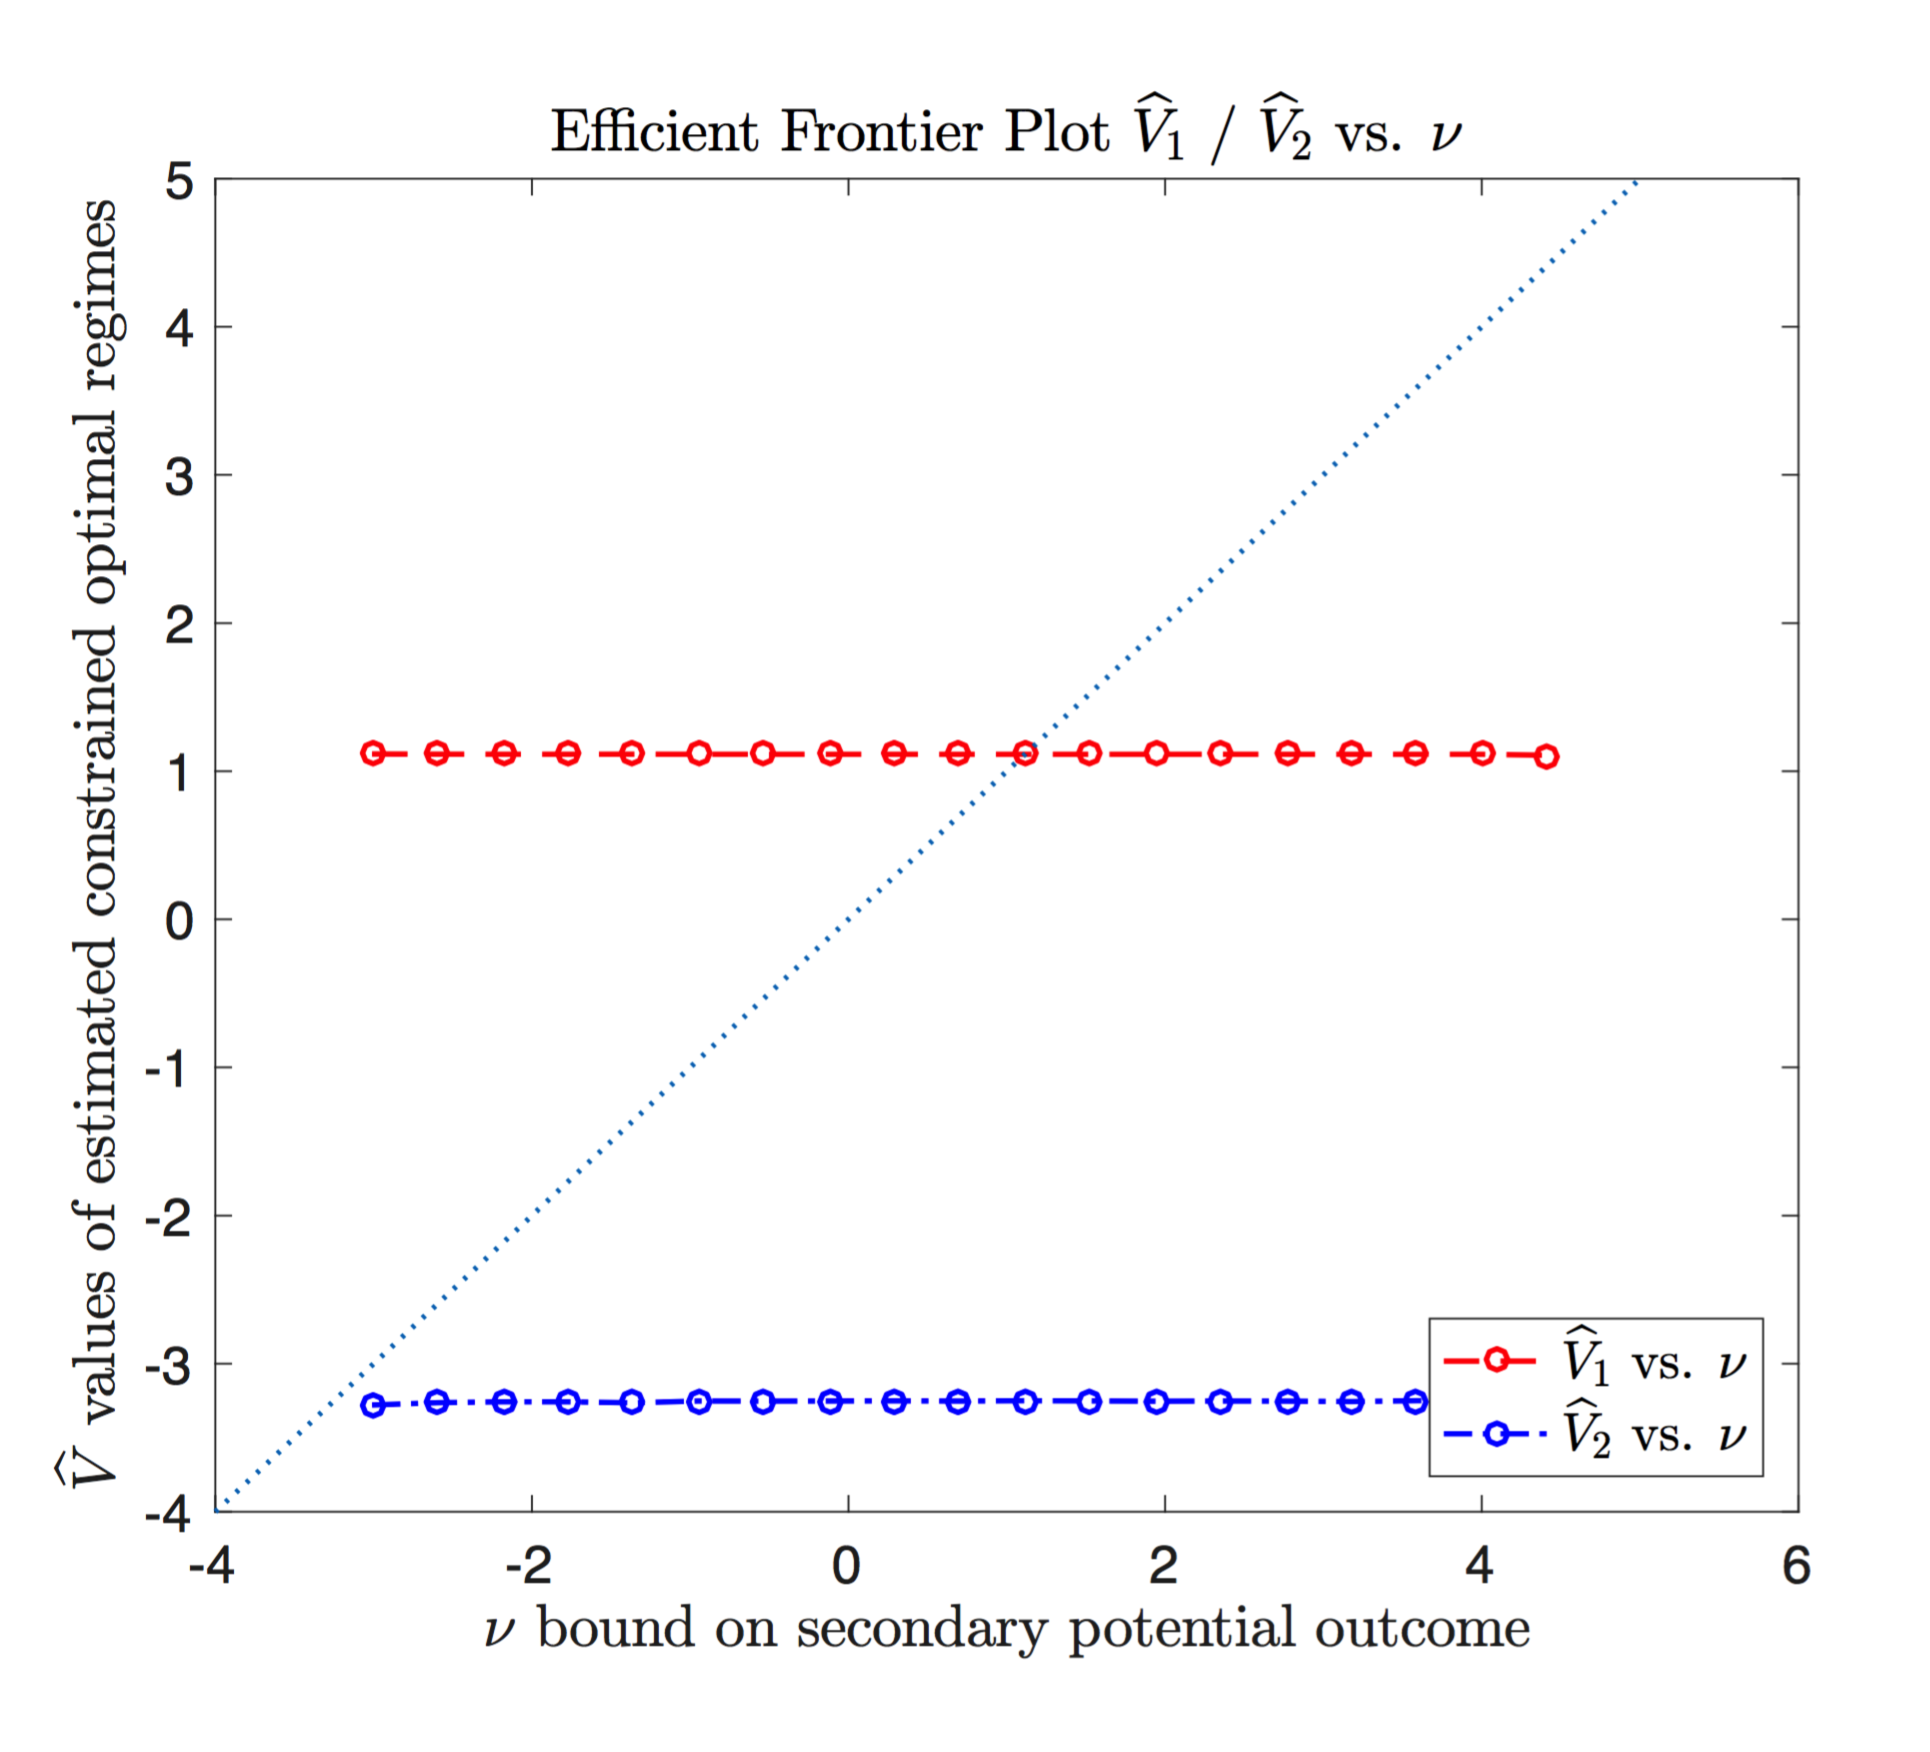
\includegraphics[width=.9\linewidth]{./Chapter-1/figs/efficient_plot7.png}
	\caption{Efficient frontier for estimated constrained optimal regimes for Setting 7.}
	\label{fig:7}
	\justify
X-axis is for the values for the constraints $\nu$; Y-axis is for the values of estimated regimes. Red dashed line is for the values in terms of the primary outcome of interest. Blue dashed line is for the values in terms of the secondary outcome of interest.
\end{figure}
\begin{table}[!htbp]
	\caption {Simulation Result for Setting 8}
	\centering
	{\tt
		\begin{tabular}{rrrrrrrrrr}\hline 
$\nu$  & $\wh{V}_1(\wh{\bs{\theta}}_{\nu})$ & $std(\wh{V}_1)$ & $\wh{V}_2(\wh{\bs{\theta}}_{\nu})$ & $std(\wh{V}_2)$ & $\wh{\theta}_{\nu,1}$ & $std(\wh{\theta}_{\nu,1})$ & $\wh{\theta}_{\nu,2}$ & $std(\wh{\theta}_{\nu,2})$ \\ \hline 
%8 &      NaN &      NaN &      NaN  &      NaN &       NaN &       NaN &       NaN &       NaN &       NaN \\ 
%8 &      NaN &      NaN &      NaN  &      NaN &       NaN &       NaN &       NaN &       NaN &       NaN \\ 
%8 &    -3.19 &      NaN &      NaN  &      NaN &       NaN &       NaN &       NaN &       NaN &       NaN \\ 
-2.80 &    -0.36 &     0.33  &    -2.85 &      0.12 &      0.78 &      0.05 &     -0.63 &      0.06 \\ 
-2.41 &     0.54 &     0.26  &    -2.44 &      0.14 &      0.64 &      0.04 &     -0.77 &      0.04 \\ 
-2.02 &     1.24 &     0.22  &    -2.05 &      0.14 &      0.51 &      0.05 &     -0.86 &      0.03 \\ 
-1.64 &     1.82 &     0.21  &    -1.66 &      0.15 &      0.39 &      0.04 &     -0.92 &      0.02 \\ 
-1.25 &     2.35 &     0.19  &    -1.24 &      0.16 &      0.27 &      0.04 &     -0.96 &      0.01 \\ 
-0.86 &     2.82 &     0.17  &    -0.84 &      0.16 &      0.15 &      0.04 &     -0.99 &      0.01 \\ 
-0.47 &     3.18 &     0.50  &    -0.44 &      0.15 &      0.05 &      0.05 &     -0.99 &      0.13 \\ 
-0.08 &     3.51 &     0.51  &    -0.08 &      0.15 &     -0.06 &      0.05 &     -0.99 &      0.13 \\ 
 0.31 &     3.75 &     0.86  &     0.30 &      0.17 &     -0.16 &      0.07 &     -0.96 &      0.24 \\ 
 0.70 &     3.92 &     1.21  &     0.71 &      0.16 &     -0.26 &      0.09 &     -0.90 &      0.33 \\ 
 1.09 &     4.16 &     1.19  &     1.10 &      0.16 &     -0.36 &      0.08 &     -0.87 &      0.33 \\ 
 1.47 &     4.30 &     1.32  &     1.51 &      0.16 &     -0.45 &      0.09 &     -0.81 &      0.37 \\ 
 1.86 &     4.22 &     1.74  &     1.88 &      0.15 &     -0.53 &      0.12 &     -0.69 &      0.48 \\ 
 2.25 &     3.73 &     2.35  &     2.26 &      0.15 &     -0.59 &      0.15 &     -0.45 &      0.65 \\ 
 2.64 &     4.44 &     1.50  &     2.65 &      0.11 &     -0.71 &      0.09 &     -0.56 &      0.42 \\ 
 3.03 &     4.79 &     0.64  &     2.74 &      0.06 &     -0.75 &      0.04 &     -0.63 &      0.19 \\ 
 3.42 &     4.67 &     0.92  &     2.76 &      0.15 &     -0.75 &      0.03 &     -0.59 &      0.30 \\ 
 3.81 &     4.81 &     0.44  &     2.75 &      0.14 &     -0.75 &      0.01 &     -0.64 &      0.16 \\ 
 4.20 &     4.85 &     0.15  &     2.74 &      0.12 &     -0.75 &      0.02 &     -0.65 &      0.07 \\ \hline 
\end{tabular}

	}
	\justify
	Here, $\nu$ denotes the values of the constraint; $\wh{V}_1(\wh{\bs{\theta}}_{\nu})$ denotes the values of estimated regimes in terms of primary outcome of interest; $std(\wh{V}_1)$ denotes the standard deviation of the estimated regime values in terms of primary outcome of interest; $\wh{V}_2(\wh{\bs{\theta}}_{\nu})$ denotes the values of estimated regimes in terms of secondary outcome of interest; $std(\wh{V}_2)$ denotes the standard deviation of the estimated regime values in terms of secondary outcome of interest; $\wh{\theta}_{\nu,1}$ and $\wh{\theta}_{\nu,2}$ denote the estimated index parameters of the regimes; $std(\wh{\theta}_{\nu,1})$ and $std(\wh{\theta}_{\nu,2})$ denote the standard deviations of those estimated index parameters.	
\end{table} 
\begin{figure}[!htb]
	\centering
	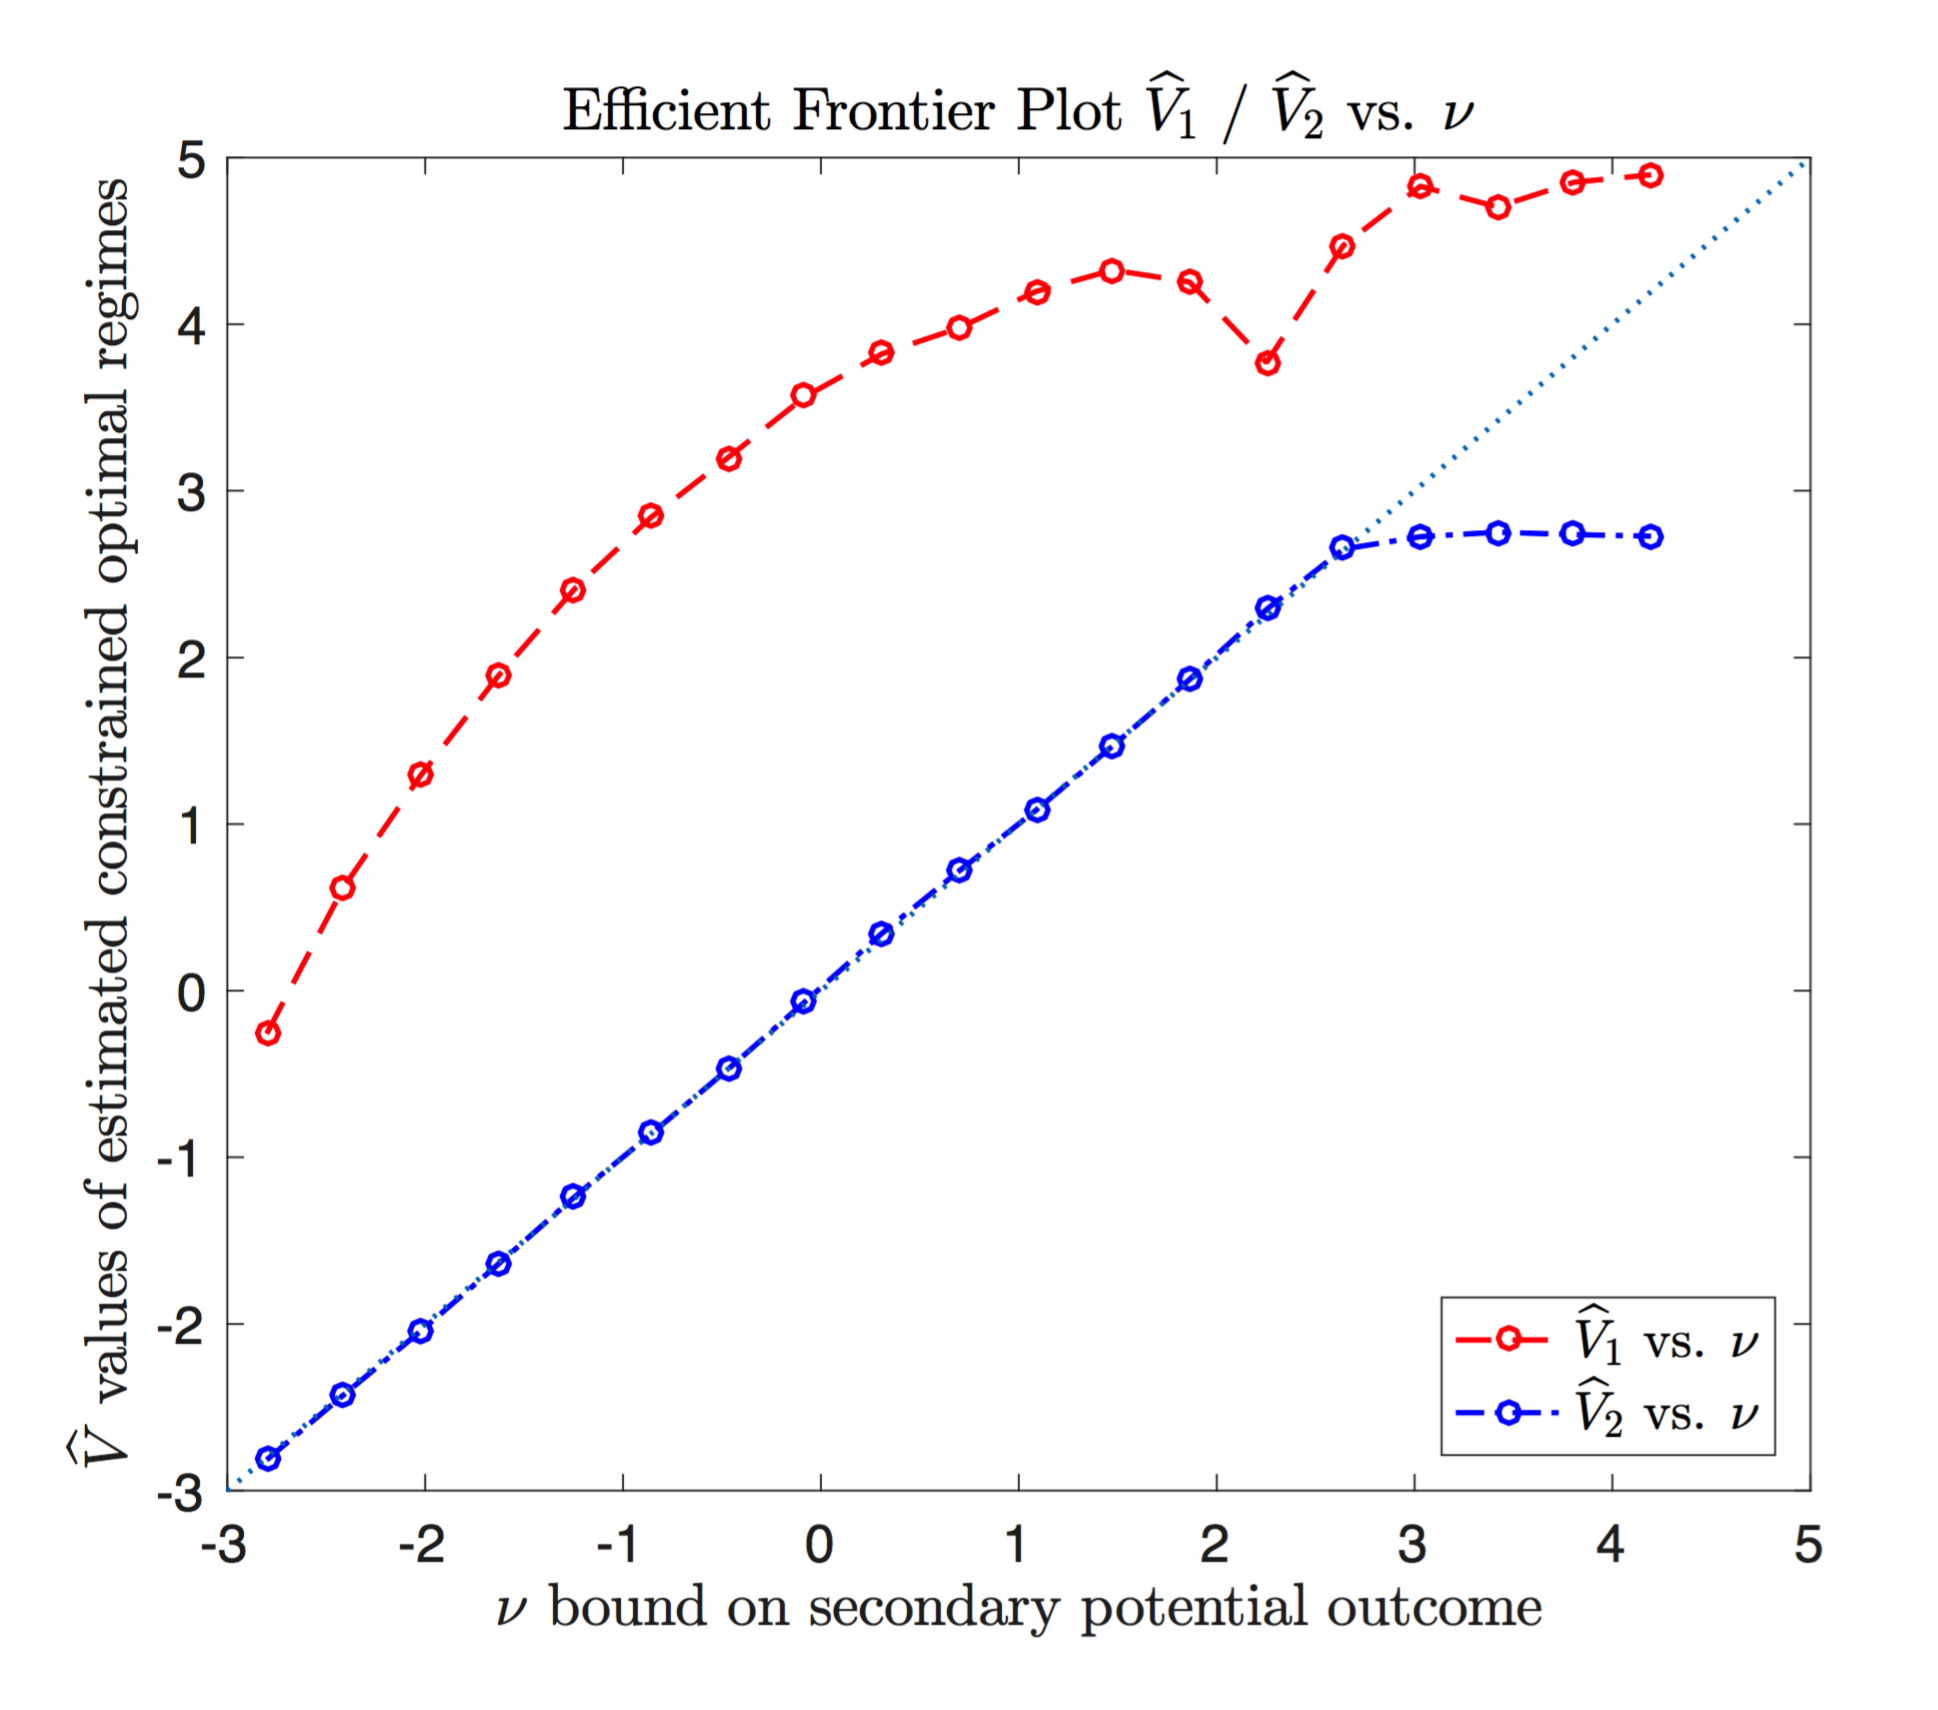
\includegraphics[width=.9\linewidth]{./Chapter-1/figs/efficient_plot8.png}
	\caption{Efficient frontier for estimated constrained optimal regimes for Setting 8.}
	\label{fig:8}
	\justify
X-axis is for the values for the constraints $\nu$; Y-axis is for the values of estimated regimes. Red dashed line is for the values in terms of the primary outcome of interest. Blue dashed line is for the values in terms of the secondary outcome of interest.
\end{figure}
\begin{table}[!htbp]
	\caption {Simulation Result for Setting 9}
	\centering
	{\tt
		\begin{tabular}{rrrrrrrrrr}\hline 
 $\nu$  & $\wh{V}_1(\wh{\bs{\theta}}_{\nu})$ & $std(\wh{V}_1)$ & $\wh{V}_2(\wh{\bs{\theta}}_{\nu})$ & $std(\wh{V}_2)$ & $\wh{\theta}_{\nu,1}$ & $std(\wh{\theta}_{\nu,1})$ & $\wh{\theta}_{\nu,2}$ & $std(\wh{\theta}_{\nu,2})$ \\ \hline 
-0.70 &     3.32 &     1.24  &    -0.97 &      0.63 &      0.75 &      0.04 &     -0.66 &      0.05 \\ 
-0.56 &     3.72 &     0.01  &    -0.77 &      0.02 &      0.73 &      0.04 &     -0.68 &      0.04 \\ 
-0.41 &     3.72 &     0.01  &    -0.77 &      0.02 &      0.73 &      0.04 &     -0.68 &      0.04 \\ 
-0.27 &     3.72 &     0.01  &    -0.77 &      0.02 &      0.73 &      0.04 &     -0.68 &      0.04 \\ 
-0.13 &     3.72 &     0.01  &    -0.77 &      0.02 &      0.73 &      0.04 &     -0.68 &      0.04 \\ 
 0.01 &     3.72 &     0.01  &    -0.77 &      0.02 &      0.73 &      0.04 &     -0.68 &      0.04 \\ 
 0.15 &     3.72 &     0.01  &    -0.77 &      0.02 &      0.73 &      0.04 &     -0.68 &      0.04 \\ 
 0.29 &     3.72 &     0.01  &    -0.77 &      0.02 &      0.73 &      0.04 &     -0.68 &      0.04 \\ 
 0.43 &     3.72 &     0.01  &    -0.77 &      0.02 &      0.73 &      0.04 &     -0.68 &      0.04 \\ 
 0.58 &     3.72 &     0.01  &    -0.77 &      0.02 &      0.73 &      0.04 &     -0.68 &      0.04 \\ 
 0.72 &     3.72 &     0.01  &    -0.77 &      0.02 &      0.73 &      0.04 &     -0.68 &      0.04 \\ 
 0.86 &     3.72 &     0.01  &    -0.77 &      0.02 &      0.73 &      0.04 &     -0.68 &      0.04 \\ 
 1.00 &     3.72 &     0.01  &    -0.77 &      0.02 &      0.73 &      0.04 &     -0.68 &      0.04 \\ 
 1.14 &     3.72 &     0.01  &    -0.77 &      0.02 &      0.73 &      0.04 &     -0.68 &      0.04 \\ 
 1.28 &     3.72 &     0.01  &    -0.77 &      0.02 &      0.73 &      0.04 &     -0.68 &      0.04 \\ 
 1.43 &     3.72 &     0.01  &    -0.77 &      0.02 &      0.73 &      0.04 &     -0.68 &      0.04 \\ 
 1.57 &     3.72 &     0.01  &    -0.77 &      0.02 &      0.73 &      0.04 &     -0.68 &      0.04 \\ 
 1.71 &     3.72 &     0.01  &    -0.77 &      0.02 &      0.73 &      0.04 &     -0.68 &      0.04 \\ 
 1.85 &     3.72 &     0.01  &    -0.77 &      0.02 &      0.73 &      0.04 &     -0.68 &      0.04 \\ \hline 
\end{tabular}

	}
	\justify
	Here, $\nu$ denotes the values of the constraint; $\wh{V}_1(\wh{\bs{\theta}}_{\nu})$ denotes the values of estimated regimes in terms of primary outcome of interest; $std(\wh{V}_1)$ denotes the standard deviation of the estimated regime values in terms of primary outcome of interest; $\wh{V}_2(\wh{\bs{\theta}}_{\nu})$ denotes the values of estimated regimes in terms of secondary outcome of interest; $std(\wh{V}_2)$ denotes the standard deviation of the estimated regime values in terms of secondary outcome of interest; $\wh{\theta}_{\nu,1}$ and $\wh{\theta}_{\nu,2}$ denote the estimated index parameters of the regimes; $std(\wh{\theta}_{\nu,1})$ and $std(\wh{\theta}_{\nu,2})$ denote the standard deviations of those estimated index parameters.	
\end{table} 
\begin{figure}[!htb]
	\centering
	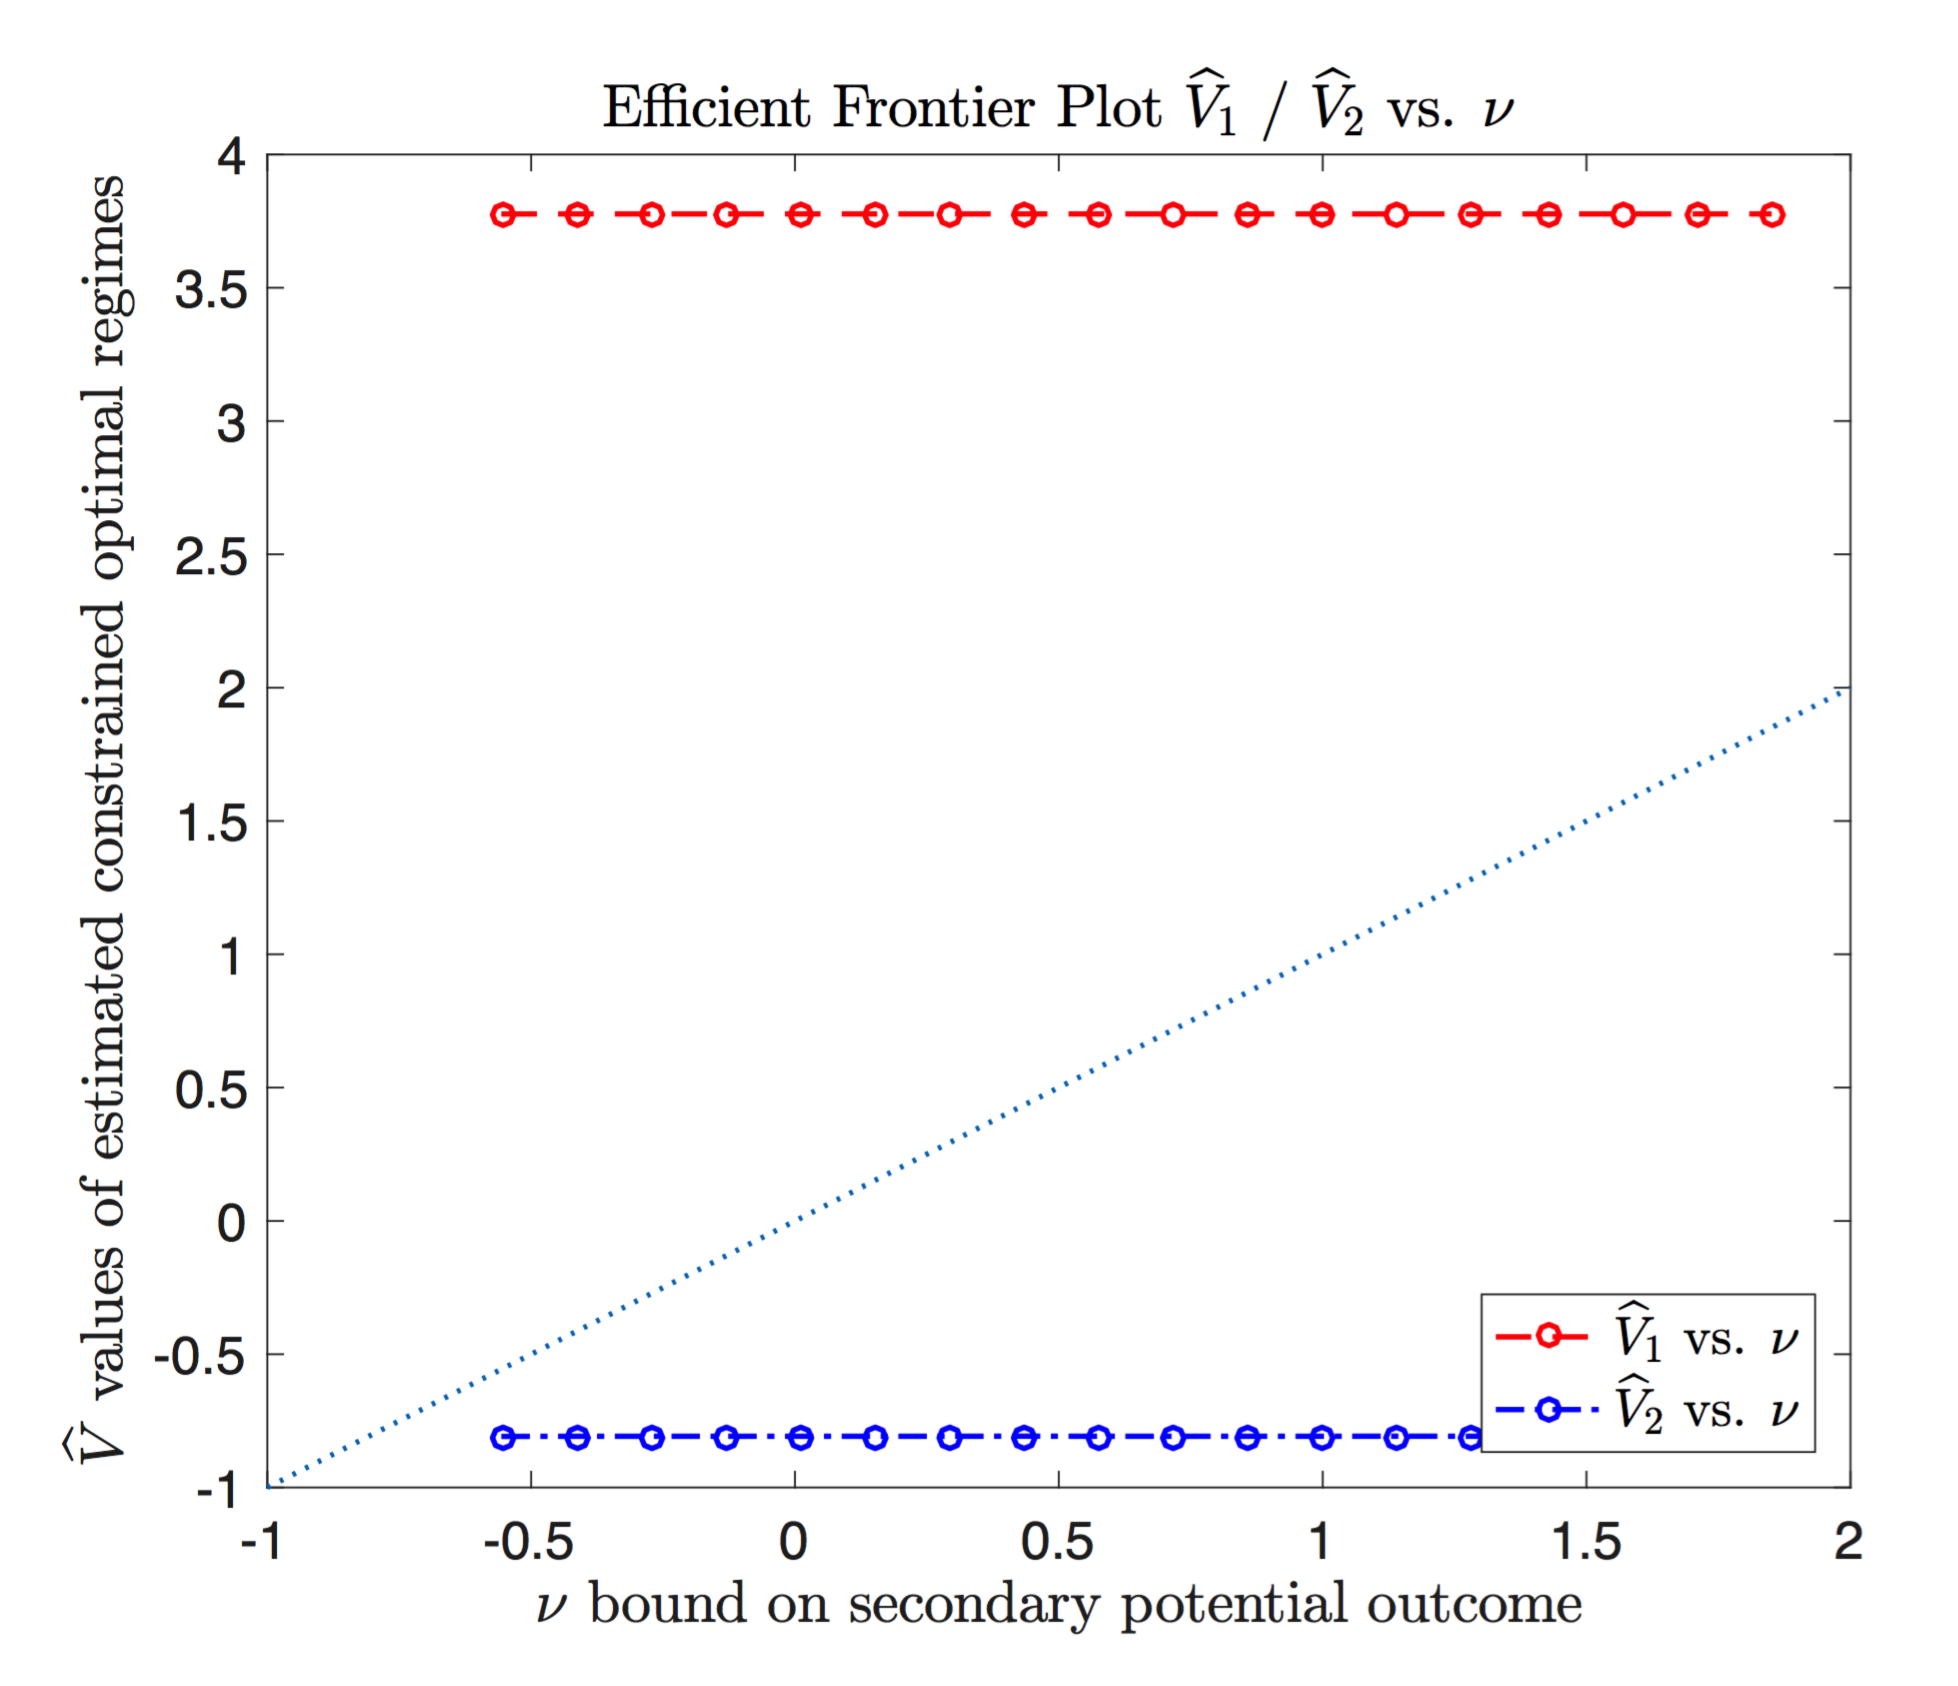
\includegraphics[width=.9\linewidth]{./Chapter-1/figs/efficient_plot9.png}
	\caption{Efficient frontier for estimated constrained optimal regimes for Setting 9.}
	\label{fig:9}
	\justify
X-axis is for the values for the constraints $\nu$; Y-axis is for the values of estimated regimes. Red dashed line is for the values in terms of the primary outcome of interest. Blue dashed line is for the values in terms of the secondary outcome of interest.
\end{figure}
%	{\centering
%		\begin{minipage}{0.45\textwidth}
%			\centering
%			%%%\includegraphics[width=.9\linewidth]{lb9.pdf}
%			\captionof{figure}{Setting 9 by log barrier method}
%		\end{minipage}
%		\begin{minipage}{0.45\textwidth}
%			\centering
%			%%%\includegraphics[width=.9\linewidth]{ex9.pdf}
%			\captionof{figure}{Setting 9 by exact penalty method}
%		\end{minipage}
%	}\\
%	
\chapter{Supplement materials for Chapter 3}
\section{Proof of Lemma 2.1.1}
\begin{lemma}
 Suppose the following conditions hold.
	\begin{enumerate}
		\item $\forall \bs{a} \in \mathbb{R}^p$,$\exists \delta > 0$ ,such that
		\begin{enumerate}
			\item $\mathbb{E}\lt|\bs{a}^\itl\pard[\bs{\theta}] \int y \,d  \wh{F}_{Y_j^*(\bs{\theta})}(y | \bs{H}_{1,i} = \bs{h}_{1,i})\rt|^{2+\delta} < \infty$
			\item $ \lt\{\bs{\bs{a}^{\intercal}}V\lt[\pard[\bs{\theta}] \int y \,d  \wh{F}_{Y_j^*(\bs{\theta})}(y | \bs{H}_{1,i} = \bs{h}_{1,i})\rt]\bs{a} \rt\}^{1+\frac{\delta}{2}}< \infty$.
		\end{enumerate}
	\end{enumerate}
	Then, we have, for any fixed $\bs{\theta}$,
	\begin{gather}
	\begin{flalign*}
	\sqrt{n}\lt(\nabla \wh{V}_j(\bs{\theta})  -\mathbb{E}\lt(\nabla \wh{V}_j(\bs{\theta})\rt)\rt)\overset{d}{\to}\mathcal{N}\lt(0,AV\lt(\pard[\bs{\theta}] \int y \,d  \wh{F}_{Y_j^*(\bs{\theta})}(y | \bs{H}_{1,i} = \bs{h}_{1,i}) \rt)\rt)
	\end{flalign*}
	\end{gather}
\end{lemma}

The proof of this is similar to the proof of Lemma 1.1.3 and is shown in APPENDIX.
%\subsection{Limiting distribution of $\nabla_{\bs{\theta}}\wh{\mathbb{E}}\lt\{ \text{sgn}\lt(\bs{X}^{\intercal}\bs{\theta}\rt)\bs{X}_1^{\intercal}\bs{\beta}_{Y1}\rt\} $}

%Comment: Goal is to prove the derivative above is asymptotically normal.
%Considering that it includes sample size $n$ in $h$, and it is multivariate.
%Try Lyapunov condition and cramer-wold theorem first.
%
%The sequences here are a triangular array, and are iid for each $n$.
%
%$k$ is the kernel of our choice, gaussian kernel.

\begin{proof}
	For any  $\bs{a} \in \mathbb{R}^p$, we let $W_{ni} = \bs{a}^\itl \pard[\bs{\theta}]\int y \,d  \wh{F}_{Y_j^*(\bs{\theta})}(y | \bs{H}_{1,i} = \bs{h}_{1,i})$. For each value of $n$, $w_{n1},w_{n2},\cdots,w_{nn}$ are i.i.d, and functions of the sample size $n$. This is because that $\bs{X}_{i}$ are assumed to be i.i.d., and $h$ is a function of sample
	size $n$. Then, we have
	\begin{gather*}
	\mu_{n}:=\mathbb{E}W_{ni}=\mathbb{E}\lt(\bs{a}^\itl \pard[\bs{\theta}]\int y \,d  \wh{F}_{Y_j^*(\bs{\theta})}(y | \bs{H}_{1,i} = \bs{h}_{1,i})\rt),
	\end{gather*}
	and
	\begin{gather*}
	\sigma_{n}^{2}:=V(W_{ni})=\bs{a}^\itl V\lt(\pard[\bs{\theta}]\int y \,d  \wh{F}_{Y_j^*(\bs{\theta})}(y | \bs{H}_{1,i} = \bs{h}_{1,i}) \rt)\bs{a}
	\end{gather*}
	
	%?????????????????????????????????????????????????????????? \\
	%??? Delta method and Taylor expansion for approximation ??? \\
	%?????????????????????????????????????????????????????????? \\
	We let $G_{ni}=W_{ni}-\mu_{\ensuremath{n}}$, and $T_{n}=\sum_{i=1}^{n}G_{ni}$. Also, we let $s_{n}^{2}=V(T_{n})=\sum_{i=1}^{n}V(G_{ni})=\sum_{i=1}^{n}\sigma_{n}^{2}=n\sigma_{n}^{2}$, where the second equality is because of independence, and the last equality is due to identicalness. Therefore, $\sfrac{T_{n}}{s_{n}}$ has mean 0, and variance 1.  If we can show $G_{ni}$ satisfying the Lyapunov condition, then
	we have
	
	$$\frac{T_{n}}{s_{n}}\overset{d}{\to}\mathcal{N}(0,1),\text{ as } n \to \infty$$,
	
	
	
	Now, we check the Lyapunov condition, that is, ~\cite{Lindsay1995,Hunter2014}
	\begin{gather*}
	\exists\delta>0, \text{ such that } \frac{1}{s_{n}^{2+\delta}}\sum_{i=1}^{n}\mathbb{E}\mid G_{n,i}\mid^{2+\delta}\to0, \text{ as } n\to0.
	\end{gather*}
	We define, for any $\bs{a}$,
	\begin{gather*}
	C_1 \triangleq \mathbb{E}\lt|G_{ni}\rt|^{2+\delta}=\mathbb{E}\lt|W_{ni}-\mu_{\ensuremath{n}}\rt|^{2+\delta}=\mathbb{E}\lt|\bs{a}^\itl \pard[\bs{\theta}]\int y \,d  \wh{F}_{Y_j^*(\bs{\theta})}(y | \bs{H}_{1,i} = \bs{h}_{1,i})-\mu_{n}\rt|^{2+\delta},
	\end{gather*}
	and
	\begin{gather*}
	C_2 \triangleq s_{n}^{2+\delta}=n^{1+\frac{\delta}{2}}\sigma_{n}^{2+\delta}=n^{1+\frac{\delta}{2}}\lt\{ \bs{a}^\itl  V \lt[ \pard[\bs{\theta}]\int y \,d  \wh{F}_{Y_j^*(\bs{\theta})}(y | \bs{H}_{1,i} = \bs{h}_{1,i}) \rt] \bs{a} \rt\} ^{1+\frac{\delta}{2}}.
	\end{gather*}
	Then, we have
	\begin{flalign*}
	&\frac{1}{s_{n}^{2+\delta}}\sum_{i=1}^{n}\mathbb{E}\mid G_{n,i}\mid^{2+\delta}\\
	=&\frac{\mathbb{E}\lt|\bs{a}^\itl \pard[\bs{\theta}]\int y \,d  \wh{F}_{Y_j^*(\bs{\theta})}(y | \bs{H}_{1,i} = \bs{h}_{1,i})-\mu_{n}\rt|^{2+\delta}}{n^{\frac{\delta}{2}}\lt\{ \bs{a}^{\intercal}V\lt[\pard[\bs{\theta}]\int y \,d  \wh{F}_{Y_j^*(\bs{\theta})}\lt(y | \bs{H}_{1,i} = \bs{h}_{1,i}\rt) \rt]\bs{a}\rt\} ^{1+\frac{\delta}{2}}} \\
	=&\frac{C_{1}}{n^{\frac{\delta}{2}}C_{2}}.
	\end{flalign*}
	
	As long as $\delta>0$, for finite $C_1$ and finite $C_2$, we have $\sfrac{C_{1}}{n^{\frac{\delta}{2}}C_{2}}\to0$,
	as $n\to\infty$. This means that the Lyapunov condition is satisfied, if $\mathbb{E}\lt|G_{ni}\rt|^{2+\delta}$ and $s_{n}^{2+\delta}$ are finite. Then,  by Lyapunov Central Limit Theorem, we have
	\begin{gather*}
	\frac{T_{n}}{s_{n}}\overset{d}{\to}\mathcal{N}(0,1).
	\end{gather*}
	
	As this hold for any arbitary non-random vector $\bs{a}\in \mathbb{R}^p$, we have, by Cramer-Wold Theorem, that
	\begin{gather*}
	\sqrt{n}\lt[\mean[n] \pard[\bs{\theta}]\int y \,d  \wh{F}_{Y_j^*(\bs{\theta})}(y | \bs{H}_{1,i} = \bs{h}_{1,i}) -\mathbb{E}\lt\{ \pard[\bs{\theta}]\int y \,d  \wh{F}_{Y_j^*(\bs{\theta})}(y | \bs{H}_{1,i} = \bs{h}_{1,i})\rt\}\rt]\overset{d}{\to}\mathcal{N}\lt(0,V\lt[\pard[\bs{\theta}]\int y \,d  \wh{F}_{Y_j^*(\bs{\theta})}(y | \bs{H}_{1,i} = \bs{h}_{1,i})\rt]\rt),
	\end{gather*}
	as $n \to \infty$. We denote $\bs{L}_{ni}= \pard[\bs{\theta}]\int y \,d  \wh{F}_{Y_j^*(\bs{\theta})}(y | \bs{H}_{1,i} = \bs{h}_{1,i})$,
	then this is written as
	\begin{gather*}
	\sqrt{n}\lt[\frac{1}{n}\sum_{i=1}^{n}\bs{L}_{ni}-\mathbb{E}\bs{L}_{n1}\rt]\overset{d}{\to}\mathcal{N}\lt(0,V\lt[\bs{L}_{n1}\rt]\rt).
	\end{gather*}
	Then, we have
	\begin{gather*}
	\frac{1/n\sum_{i=1}^{n}\bs{L}_{ni}-\mathbb{E}\bs{L}_{n1}}{[V(\bs{L}_{n1})/n]^{1/2}}\frac{[V(\bs{L}_{n1})/n]^{1/2}}{\lt[AV(\bs{L}_{n1})/n\rt]^{1/2}}\overset{d}{\to}\mathcal{N}(0,1).
	\end{gather*}
	As  $n \to \infty$,
	\begin{gather*}
	\frac{V(\bs{L}_{n1})^{1/2}}{AV(\bs{L}_{n1})^{1/2}}\to1,
	\end{gather*}
	then we have
	\begin{gather*}
	\frac{1/n\sum_{i=1}^{n}\bs{L}_{ni}-\mathbb{E}\bs{L}_{n1}}{[AV(\bs{L}_{n1})/n]^{1/2}}\overset{d}{\to}\mathcal{N}(0,1),
	\end{gather*}
	i.e.,
	\begin{gather*}
	\sqrt{n}\lt[1/n\sum_{i=1}^{n}\bs{L}_{ni}-\mathbb{E}\bs{L}_{n1}\rt]\overset{d}{\to}N\lt(0,AV(\bs{L}_{n1})\rt).
	\end{gather*}
	As $\frac{1}{n}\sum_{i=1}^{n}\bs{L}_{ni} =\mean[n] \pard[\bs{\theta}]\int y \,d  \wh{F}_{Y_j^*(\bs{\theta})}(y | \bs{H}_{1,i} = \bs{h}_{1,i}) = \nabla \wh{V}_j(\bs{\theta})$, we have
	\begin{gather}
	\begin{flalign*}
	\sqrt{n}\lt[\nabla \wh{V}_j(\bs{\theta})  -\mathbb{E}\lt\{\nabla \wh{V}_j(\bs{\theta})\rt\}\rt]\overset{d}{\to}\mathcal{N}\lt(0,AV\lt[\pard[\bs{\theta}] \int y \,d  \wh{F}_{Y_j^*(\bs{\theta})}(y | \bs{H}_{1,i} = \bs{h}_{1,i}) \rt]\rt)
	\end{flalign*}
	\end{gather}
\end{proof}
\section{Proof of Corollary 2.1.2}
\begin{corollary}
	Suppose all the assumptions in Lemma 3  hold, and $\wh{F}_{Y_j^*(\bs{\theta})}(y | \bs{H}_{1,i} = \bs{h}_{1,i})$ is a consistent estimator of ${F}_{Y_j^*(\bs{\theta})}(y_j | \bs{H}_{1,i} = \bs{h}_{1,i})$. Then, we have
	\begin{gather}
	\begin{flalign*}
	\sqrt{n}\lt(\nabla \wh{V}_j(\bs{\theta}^*_{\bs{\nu}}(\mu))  - \nabla V_j(\bs{\theta}^*_{\bs{\nu}}(\mu))\rt)\overset{d}{\to}\mathcal{N}\lt(0,AV\lt(\pard[\bs{\theta}] \int y_j \,d  F_{Y_j^*(\bs{\theta})}(y | \bs{H}_{1,i} = \bs{h}_{1,i})\bigg\rvert_{\bs{\theta} = \bs{\theta}^*_{\bs{\nu}}(\mu)} \rt)\rt)
	\end{flalign*}
	\end{gather}
\end{corollary}
\begin{proof}
	We write
	\begin{gather}
	\begin{flalign*}
	& \nabla \wh{V}_j(\bs{\theta})  - \nabla V_j^*(\bs{\theta}) \\
	= & \nabla \wh{V}_j(\bs{\theta})  - \mb{E}\lt(\nabla \wh{V}_j(\bs{\theta}) \rt) + \mb{E}\lt(\nabla \wh{V}_j(\bs{\theta}) \rt)- \nabla V_j^*(\bs{\theta}) ,
	\end{flalign*}
	\end{gather}
	where $ \mb{E}\lt(\nabla \wh{V}_j(\bs{\theta}) \rt)- \nabla V_j^*(\bs{\theta})=  \mb{E}\lt(\pard[\bs{\theta}]\int y_j \,d  \wh{F}_{Y_j^*(\bs{\theta})}(y | \bs{H}_{1,i} = \bs{h}_{1,i})\rt)  - $\\$\mb{E} \lt(\pard[\bs{\theta}]\int y_j \,d  F_{Y_j^*x(\bs{\theta})}(y_j| \bs{H}_{1,i} = \bs{h}_{1,i}\rt)$  $ = o_p(1)$, due to the consistency of $\wh{F}_{Y_j^*(\bs{\theta})}(y | \bs{H}_{1,i} = \bs{h}_{1,i})$ and dominated convergence theorem.\\
	
	In lemma 2.1.1, let $\bs{\theta} = \bs{\theta}^*_{\bs{\nu}}(\mu)$ and then
	\begin{gather}
	\begin{flalign*}
	\sqrt{n}\lt(\nabla \wh{V}_j(\bs{\theta}^*_{\bs{\nu}}(\mu))  - \nabla \mb{E}\lt( \wh{V}_j(\bs{\theta}^*_{\bs{\nu}}(\mu))\rt)\rt)\overset{d}{\to}\mathcal{N}\lt(0,AV\lt(\pard[\bs{\theta}] \int y_j \,d \wh{F}_{Y_j^*(\bs{\theta})}(y | \bs{H}_{1,i} = \bs{h}_{1,i})\bigg\rvert_{\bs{\theta} = \bs{\theta}^*_{\bs{\nu}}(\mu)} \rt)\rt).
	\end{flalign*}
	\end{gather}
	As $\wh{F}_{Y_j^*(\bs{\theta})}(y | \bs{H}_{1,i} = \bs{h}_{1,i})$ is consistent, we have
	\begin{gather*}
	\frac{AV\lt[\pard[\bs{\theta}] \int y \,d  \wh{F}_{Y_j^*(\bs{\theta})}(y | \bs{H}_{1,i} = \bs{h}_{1,i}) \rt]}{AV\lt[\pard[\bs{\theta}] \int y_j \,d  F_{Y^*(\bs{\theta})}(y | \bs{H}_{1,i} = \bs{h}_{1,i}) \rt]} \overset{p}{\to} 1.
	\end{gather*}
	Then, we have
	\begin{gather}
	\begin{flalign*}
	\sqrt{n}\lt(\nabla \wh{V}_j(\bs{\theta}^*_{\bs{\nu}}(\mu))  - \nabla V_j\lt(\bs{\theta}^*_{\bs{\nu}}(\mu)\rt)\rt)\overset{d}{\to}\mathcal{N}\lt(0,AV\lt(\pard[\bs{\theta}] \int y_j \,d F_{Y_j^*(\bs{\theta})}(y | \bs{H}_{1,i} = \bs{h}_{1,i})\bigg\rvert_{\bs{\theta} = \bs{\theta}^*_{\bs{\nu}}(\mu)} \rt)\rt).
	\end{flalign*}
	\end{gather}
\end{proof}

\section{Proof of Theorem 2.1.3}
\begin{theorem}
	Suppose all the assumptions above hold. Then we have, as $n\to \infty$
	\begin{flalign*}
	\sqrt{n}\lt(\wh{\bs{\theta}}_{\bs{\nu}}(\mu) - \bs{\theta}_{\bs{\nu}}(\mu)^*\rt) \overset{d}{\to} \mathcal{N}\lt(\bs{0}, \bs{\Sigma}^* \rt),
	\end{flalign*}
	where $\bs{\Sigma}^* = \bs{D}^{*-1}\bs{C}^{*}\bs{D}^{*-1}$, 	\\$\bs{C}^* =\mathbb{E}\lt( \nabla v_1\lt(\bs{\theta}^*_{\bs{\nu}}(\mu)\rt)\nabla^{\itl} v_1\lt(\bs{\theta}^*_{\bs{\nu}}(\mu)\rt) \rt) - \mathbb{E}\lt(\nabla v_1\lt(\bs{\theta}^*_{\bs{\nu}}(\mu)\rt)\rt) \mathbb{E}\lt(\nabla^{\itl} v_1\lt(\bs{\theta}^*_{\bs{\nu}}(\mu)\rt)\rt)$,\\
	and $\bs{D}^*  =  \nabla^2 \phi^{BP}_{\mu}(\bs{\theta}^*_{\bs{\nu}}(\mu))$.
\end{theorem}
\begin{proof} For notation simplicity in this proof, let $\phi\lt(\bs{\theta}\rt) = \phi^{PB}_{\mu}\lt(\bs{\theta}\rt)$ and $\wh{\phi}(\bs{\theta}) = \wh{\phi}^{PB}_{\mu}\lt(\bs{\theta}\rt)$ for this proof. Also, let $\bs{\theta}^* = \bs{\theta}^*_{\nu}(\mu)$ and $\wh{\bs{\theta}} = \wh{\bs{\theta}}_{\nu}(\mu)$ here.
	Recall $ \wh{\phi}(\bs{\theta}) = \wh{v}_1(\bs{\theta}) - \mu \sum_{j=2}^J \ln \wh{v}_j(\bs{\theta}) + \frac{1}{2\mu}\sum_{t=1}^{T}(\bs{\theta}^{\itl}_t\bs{\theta}_t - 1)^2$.  As  $\bs{\theta}_t^{\itl}\bs{\theta}_t-1=0$ is always satisfied as a constraint, the gradient is $\nabla\wh{\phi}\lt(\bs{\theta}\rt) = \,\,\nabla\wh{v}_1(\bs{\theta}) - \mu \sum_{j=2}^J \sfrac{\nabla\wh{v}_j\lt( \bs{\theta}\rt)}{\wh{v}_j\lt( \bs{\theta}\rt)}$. Taylor expansion of $\nabla\wh{\phi}\lt(\bs{\theta}^*\rt)$ at $\bs{\theta} = \widehat{\bs{\theta}}$ shows that
	\begin{flalign*}
	\nabla\wh{\phi}\lt(\bs{\theta}^*\rt) =  \nabla\wh{\phi}(\wh{\bs{\theta}})- \nabla^2\wh{\phi}(\tilde{\bs{\theta}}) (\widehat{\bs{\theta}} - \bs{\theta}^{*}) + o_p(1),
	\end{flalign*}
	where $\tilde{\bs{\theta}}$ is between $\wh{\bs{\theta}}$ and $\bs{\theta}^*$. As $\widehat{\bs{\theta}}$ is the maximizer of $\widehat{\phi}\lt(\bs{\theta}\rt)$, it satisfies the first order condition that $\nabla \wh{\phi}(\widehat{\bs{\theta}}) = 0$. Therefore, 
	\begin{flalign}
	\sqrt{n}\nabla\wh{\phi}\lt(\bs{\theta}^*\rt) =   - \sqrt{n} \nabla^2\wh{\phi}( \tilde{\bs{\theta}}) (\widehat{\bs{\theta}} - \bs{\theta}^{*}),
	\end{flalign}
	where $\nabla\wh{\phi}\lt(\bs{\theta}\rt) = \,\,\nabla\wh{v}_1(\bs{\theta}) - \mu \sum_{j=2}^J \sfrac{\nabla\wh{v}_j\lt( \bs{\theta}\rt)}{\wh{v}_j\lt( \bs{\theta}\rt)}$.
	Recall $v_1\lt(\bs{\theta}\rt)=- V_1\lt(\bs{\theta}\rt)$ and  $v_j\lt(\bs{\theta}\rt) = V_j\lt(\bs{\theta}\rt) - \nu_j$, for $j = 2, \cdots, J$.  Due to Corollary 2.1.2, together with (A.4) and (A.5),
	\begin{flalign}
	\sqrt{n}\bigg(\nabla\wh{v}_1(\bs{\theta}^*) - \nabla v_1(\bs{\theta}^*)\bigg)\overset{d}{\to}N\lt( 0, \bs{C}^*\rt),
	\end{flalign}
		where $\bs{C}^*=AV\bigg(\nabla v_1(\bs{\theta}^*)\bigg) =\mathbb{E}\lt\{  \nabla v_1(\bs{\theta}^*)\nabla^{\itl} v_1(\bs{\theta}^*) \rt\} - \mathbb{E}\nabla v_1(\bs{\theta}^*) \mathbb{E}\nabla^{\itl} v_1(\bs{\theta}^*)$\\
		$ = AV\lt(\pard[\bs{\theta}]\int y \,d  F_{Y_j^*(\bs{\theta})}(y | \bs{H}_{1,i} )\rt)$. That is,
%	\begin{gather*}
%	\begin{flalign*}
%	\bs{C}^* \triangleq =&AV\bigg(\nabla v_1(\bs{\theta}^*)\bigg)=
%	AV\lt[\frac{2\bs{X}_1^{\itl}\bs{\beta}^*_{1}}{h}k\lt(-\frac{\bs{X}^{\itl}\bs{\theta}^*}{h}\rt)\bs{X} \rt] = p\lim_{n \to \infty} V\lt[\frac{2\bs{X}_1^{\itl}\bs{\beta}^*_{1}}{h}k\lt(-\frac{\bs{X}^{\itl}\bs{\theta}^*}{h}\rt)\bs{X} \rt] \\
%	= & p\underset{n \to \infty}\lim \lt[ \mathbb{E} \lt\{ \frac{4\bs{\beta}^{*\itl}_{1}\bs{X}_1\bs{X}_1^{\itl}\bs{\beta}^*_{1}}{h^2}k^2\lt(-\frac{\bs{X}^{\itl}\bs{\theta}^*}{h}\rt)\bs{X}\bs{X}^{\itl}\rt\} -  \mathbb{E}\lt\{\frac{2\bs{X}_1^{\itl}\bs{\beta}^*_{1}}{h}k\lt(-\frac{\bs{X}^{\itl}\bs{\theta}^*}{h}\rt)\bs{X}\rt\} \mathbb{E}\lt\{\frac{2\bs{X}_1^{\itl}\bs{\beta}^*_{1}}{h}k\lt(-\frac{\bs{X}^{\itl}\bs{\theta}^*}{h}\rt)\bs{X}\rt\}^{\itl} \rt] \\
%	= & \mathbb{E}\lt\{  4\big(\bs{X}_1^{\itl}\bs{\beta}^*_{1}\delta\lt(\bs{X}^{\itl}\bs{\theta}^*\rt)\big)^2\bs{X}\bs{X}^{\itl} \rt\} - \mathbb{E}\lt\{2\bs{X}_1^{\itl}\bs{\beta}^*_{1}\delta\lt(\bs{X}^{\itl}\bs{\theta}^*\rt)\bs{X}\rt\} \mathbb{E}\lt\{2\bs{X}_1^{\itl}\bs{\beta}^*_{1}\delta\lt(\bs{X}^{\itl}\bs{\theta}^*\rt)\bs{X}\rt\}^{\itl}\\
%	=& \mathbb{E}\lt\{  \nabla v_1(\bs{\theta}^*)\nabla^{\itl} v_1(\bs{\theta}^*) \rt\} - \mathbb{E}\lt\{\nabla v_1(\bs{\theta}^*)\rt\} \mathbb{E}\lt\{\nabla^{\itl} v_1(\bs{\theta}^*)\rt\}.
%	\end{flalign*}
%	\end{gather*}
	Then, due to (B.1) and (B.2), we have
	\begin{flalign}
	\sum_{j=2}^J \frac{\nabla\wh{v}_j\lt( \bs{\theta}\rt)}{\wh{v}_j\lt( \bs{\theta}\rt)} -  \sum_{i=2}^{J}\frac{\nabla v_j(\bs{\theta})}{v_j(\bs{\theta})} = o_p(1).
	\end{flalign}
	Note $v_j(\bs{\theta}) > 0$, for $j =2, \cdots, J$, is implied by the log barrier operator. Put (B.2) and (B.3) together by Slutsky's theorem, we have
	\begin{flalign*}
	\sqrt{n}\lt\{\lt(\nabla\wh{v}_1(\bs{\theta}^*) - \mu \sum_{j=2}^J \frac{\nabla\wh{v}_j\lt( \bs{\theta}^*\rt)}{\wh{v}_j( \bs{\theta}^*)}\rt) - \lt(\nabla v_1(\bs{\theta}^*) - \mu \sum_{i=2}^{J}\frac{\nabla v_j(\bs{\theta}^*)}{v_j(\bs{\theta}^*)}\rt)\rt\}\overset{d}{\to}N\lt(0, \bs{C}^*\rt),
	\end{flalign*} 
	Due to the stationarity of $\bs{\theta}^*$, $\nabla \phi(\bs{\theta}^*)=\nabla v_1(\bs{\theta}^*) - \mu \sum_{i=2}^{J}\sfrac{\nabla v_j(\bs{\theta}^*)}{v_j(\bs{\theta}^*)} =0$. Together with Sluskty's theorem, we have 
	\begin{flalign*}
	\sqrt{n} \nabla\wh{\phi}( \bs{\theta}^*) \overset{d}{\to} N\lt(0, \bs{C}^*\rt),
	\end{flalign*}
	where 
	$\bs{C}^* =\mathbb{E}\lt\{  \nabla v_1(\bs{\theta}^*)\nabla^{\itl} v_1(\bs{\theta}^*) \rt\} - \mathbb{E}\lt\{\nabla v_1(\bs{\theta}^*)\rt\} \mathbb{E}\lt\{\nabla^{\itl} v_1(\bs{\theta}^*)\rt\}.$ \\
	
	As $	\sqrt{n}\nabla\wh{\phi}\lt(\bs{\theta}^*\rt) =  - \sqrt{n} \nabla^2\wh{\phi}( \tilde{\bs{\theta}}) (\widehat{\bs{\theta}} - \bs{\theta}^{*})$ stated in (A.7),we have
	\begin{flalign}
	\sqrt{n} \nabla^2\wh{\phi}( \tilde{\bs{\theta}}) (\widehat{\bs{\theta}} - \bs{\theta}^{*}) \overset{d}{\to} N(0, \bs{C}^*)
	\end{flalign} 	
	The Hessian is $\nabla^2\wh{\phi}\lt(\bs{\theta}\rt) = \,\,\nabla^2\wh{v}_1(\bs{\theta}) - \mu \sum_{j=2}^J \sfrac{\big(\nabla^2\wh{v}_j\lt( \bs{\theta}\rt)\wh{v}_j\lt( \bs{\theta}\rt)- \lt(\nabla\wh{v}_j\lt( \bs{\theta}\rt)\rt)^2\big)}{\wh{v}^2_j\lt( \bs{\theta}\rt)}$. Based on (A.4) and (A.5), we have
	\begin{gather}
	\begin{flalign}
	\bs{D}^* \triangleq & p\lim_{n \to \infty}\nabla^2\wh{\phi}\lt(\bs{\theta}^*\rt) =  \nabla^2 \phi(\bs{\theta}^*)
	=\nabla^2{v}_1(\bs{\theta}^*) - \mu \sum_{j=2}^J \frac{\nabla^2{v}_j\lt( \bs{\theta}^*\rt)v_j\lt( \bs{\theta}^*\rt)- \lt\{\nabla v_j\lt( \bs{\theta}^*\rt)\rt\}^2}{v^2_j\lt( \bs{\theta}^*\rt)}.
	\end{flalign}
	\end{gather}
	
	As $\tilde{\bs{\theta}}$ is a vector in-between $\bs{\theta}^*$ and $\wh{\bs{\theta}}$, we have $\nabla^2\wh{\phi}(\tilde{\bs{\theta}}) = \nabla^2\wh{\phi}(\bs{\theta}^*) + o_p(1)$. Therefore, based on (A.10) and (A.11), we have 
	\begin{flalign*}
	\sqrt{n}\lt(\widehat{\bs{\theta}} - \bs{\theta}^*\rt) \overset{d}{\to} N\lt(\bs{0}, \bs{\Sigma}^* \rt),
	\end{flalign*}
	where $\bs{\Sigma}^* = \bs{D}^{*-1}\bs{C}^{*}\bs{D}^{*-1}$, 
	$\bs{C}^* =\mathbb{E}\lt\{  \nabla v_1(\bs{\theta}^*)\nabla^{\itl} v_1(\bs{\theta}^*) \rt\} - \mathbb{E}\nabla v_1(\bs{\theta}^*) \mathbb{E}\nabla^{\itl} v_1(\bs{\theta}^*)$ and $\bs{D}^*  =  \nabla^2 \phi(\bs{\theta}^*)$.
\end{proof}
%\chapter{Supplement materials for Chapter 5}
\section{Least-squares policy evaluation (LSQ) algorithm}
\begin{algorithm}[H]
	\caption{LSQ}
	$A \leftarrow 0$ \\
	$b \leftarrow 0$ \\
	for each $(s,a, s^{\prime}, r)$
	
	\hspace{25pt} $A \leftarrow A + \phi(s,a)\lt(\phi(s,a) - \gamma \phi(s',\pi(s')\rt)^\intercal $
	
	\hspace{25pt} $b \leftarrow  b + \phi(s,a)r$
	
	$w	\leftarrow A^{-1}b$
	
	return $w$
\end{algorithm}

%%---------------------------------------------------------------------------%%
\backmatter


\end{document}
